
\documentclass[11pt,oneside,a4paper]{book}  % article ctexart book

%%%%%%%%%%%%%%%%%%%%%%%%%%%%%%%%%%%%%%%%%%%%%%%%%%%
%                  1. Package
%%%%%%%%%%%%%%%%%%%%%%%%%%%%%%%%%%%%%%%%%%%%%%%%%%%
% \usepackage{ctex} % chinese
\usepackage{geometry}
\usepackage{fancyhdr} % header and footer
\usepackage{graphicx} % insert fig

\usepackage[
%ragged
%raggedright
%raggedleft
]{sidecap}
\sidecaptionvpos{figure}{t} % caption on the side
\usepackage{pdfpages} % insert pdf
\usepackage{multicol} % muti-column
\usepackage{multirow} 
\usepackage{setspace} % line spacing
\usepackage{makeidx} % index
\usepackage{tikz} % plot env
\usepackage{indentfirst} % \chapter、\section indentation for the first line
\usepackage{caption,subcaption}  % title and subtitle
\usepackage{amsmath,amsthm,amssymb,amsfonts,mathrsfs} % math
\usepackage{siunitx}  % SI unit
\usepackage{pifont} % special symbol
\usepackage{hyperref} % link
\usepackage{cleveref}
\usepackage{booktabs} % three line table
\usepackage{tabularx} % three line table
\usepackage{longtable}
\usepackage[ruled,linesnumbered]{algorithm2e}  % algorithm
\usepackage[shortlabels]{enumitem} % list env
\usepackage{xcolor} % font color
\usepackage{graphbox} % figure position
%\usepackage{minted} % code style
% \usepackage{listings} % code style (not recommended)
\usepackage{environ}
\usepackage{mdframed}
\usepackage{bm}

%\usepackage{natbib}
%\bibliographystyle{unsrt} %  abbrv


\usepackage[autostyle]{csquotes}
\usepackage[style=alphabetic,citestyle=alphabetic,sortcites=true, autopunct=true,autolang=hyphen,hyperref=true,abbreviate=true,backref=false, backend=biber,defernumbers=true, doi=false, url=false, giveninits=true]{biblatex}
\addbibresource{bib/pub.bib}
\addbibresource{bib/refs.bib}
\addbibresource{bib/rik.bib}

\usepackage[toc,page,title,titletoc]{appendix} % appendix

\usepackage{bookmark}
\usepackage{afterpage} % blank pages


%\usepackage{titlesec}    % Remove the text 'Chapter' from each chapter.
% \titleformat{\chapter}{\normalfont\huge\bf}{\thechapter}{20pt}{\huge\bf}


%%%%%%%%%%%%%%%%%%%%%%%%%%%%%%%%%%%%%%%%%%%%%%%%%%%
%                  2. Page Setting
%%%%%%%%%%%%%%%%%%%%%%%%%%%%%%%%%%%%%%%%%%%%%%%%%%%
% margin
\geometry{left=2.5cm,right=2.5cm,top=2.5cm,bottom=2.5cm}

% footer and header
\pagestyle{fancy}
\fancyfoot[C]{\thepage}
\fancyhead[L]{\nouppercase{\leftmark}}
\fancyhead[R]{\nouppercase{\rightmark}}
\renewcommand{\headrulewidth}{1.5pt}

% spacing
\linespread{1.2}  % line spacing || 1.2 times font size
\setlength{\parindent}{2em} % indentation for the first line
\setlength{\parskip}{1ex} % spacing for each paragraph
\setlength{\headsep}{1.5\baselineskip}

% link color
\hypersetup{
    colorlinks = true,
    citecolor = blue, % References
    linkcolor = black,
    filecolor = magenta,
    urlcolor = {blue!40!black},
}





%%%%%%%%%%%%%%%%%%%%%%%%%%%%%%%%%%%%%%%%%%%%%%%%%%%
%                  3. Plot Env
%%%%%%%%%%%%%%%%%%%%%%%%%%%%%%%%%%%%%%%%%%%%%%%%%%%
\usetikzlibrary{trees,positioning,fit,calc}
\tikzset{block/.style = {draw, fill=blue!20, rectangle,
                         minimum height=3em, minimum width=4em},
        input/.style = {coordinate},
        output/.style = {coordinate}
}






%%%%%%%%%%%%%%%%%%%%%%%%%%%%%%%%%%%%%%%%%%%%%%%%%%%
%                  4. Question Env
%%%%%%%%%%%%%%%%%%%%%%%%%%%%%%%%%%%%%%%%%%%%%%%%%%%
\newenvironment{problem}[2][Problem]
    {\begin{mdframed}[backgroundcolor=gray!10] \textbf{#1 #2} \\}
    {\end{mdframed}}

\newenvironment{solution}{\textbf{Solution}}

%%%%%%%%%%%%%%%%%%%%%%%%%%%%%%%%%%%%%%%%%%%%%%%%%%%
%                  4. Abstract Env
%%%%%%%%%%%%%%%%%%%%%%%%%%%%%%%%%%%%%%%%%%%%%%%%%%%
%\newenvironment{abstract}
%    {\begin{quote}{\small \centering
%    \textbf{Abstract
%
%    }\small\itshape } \\}
%    {\end{quote}}
\newenvironment{abstract}{%
    \small
    \begin{center}%
        {\bfseries Abstract}%
    \end{center}%
    \quotation\itshape}
    {\endquotation}




%%%%%%%%%%%%%%%%%%%%%%%%%%%%%%%%%%%%%%%%%%%%%%%%%%%
%                  6. Fig Env
%%%%%%%%%%%%%%%%%%%%%%%%%%%%%%%%%%%%%%%%%%%%%%%%%%%
\graphicspath{figures/}
\captionsetup[figure]{
  labelfont={bf},
  labelformat={default},
  name={Figure},
  labelsep=colon
}

% Centering the figures
\makeatletter
\g@addto@macro\@floatboxreset\centering
\makeatother






%%%%%%%%%%%%%%%%%%%%%%%%%%%%%%%%%%%%%%%%%%%%%%%%%%%
%                 7. Footnote Env
%%%%%%%%%%%%%%%%%%%%%%%%%%%%%%%%%%%%%%%%%%%%%%%%%%%
% \interfootnotelinepenalty=10000 % 禁止脚注显示在第二页
% % redefine footnote as circled number: ①②③④⑤⑥⑦⑧⑨
% \renewcommand{\thefootnote}{\ding{\numexpr171+\value{footnote}}}


%%%%%%%%%%%%%%%%%%%%%%%%%%%%%%%%%%%%%%%%%%%%%%%%%%%
%                 8. Dedication Env
%%%%%%%%%%%%%%%%%%%%%%%%%%%%%%%%%%%%%%%%%%%%%%%%%%%
\newenvironment{dedication}
  {\clearpage           % we want a new page
   \thispagestyle{empty}% no header and footer
   \vspace*{\stretch{1}}% some space at the top
   \itshape             % the text is in italics
   \raggedleft          % flush to the right margin
  }
  {\par % end the paragraph
   \vspace{\stretch{3}} % space at bottom is three times that at the top
   \clearpage           % finish off the page
  }


%%%%%%%%%%%%%%%%%%%%%%%%%%%%%%%%%%%%%%%%%%%%%%%%%%%
%                 8. Appendix Env
%%%%%%%%%%%%%%%%%%%%%%%%%%%%%%%%%%%%%%%%%%%%%%%%%%%

\AtBeginEnvironment{subappendices}{%
\chapter*{Appendices}
%\addcontentsline{toc}{section}{Appendices}
\pdfbookmark[section]{Appendices}{toc}
\counterwithin{figure}{section}
\counterwithin{table}{section}

\hypersetup{bookmarksdepth=-1}
}

\AtEndEnvironment{subappendices}{%
\hypersetup{bookmarksdepth}
}

  
%%%%%%%%%%%%%%%%%%%%
%% PRIVATE MACROS %%
%%%%%%%%%%%%%%%%%%%%

\newcommand{\figwidth}{0.55 \columnwidth}
\newcommand{\eq}[1]{Eq.~(\ref{#1})}
\newcommand{\eqs}[1]{Eqs.~(\ref{#1})}
\newcommand{\fig}[1]{Fig.~\ref{#1}}
\newcommand{\avg}[1]{ {\langle #1 \rangle} }
\newcommand{\sect}[1]{Section~\ref{#1}}


\newcommand{\oma}{{\bf \hat{u}}}
\newcommand{\omb}{{\bf \hat{u}^{\prime}} }


\newcommand{\bs}{ {\bf s }}

\DeclareMathOperator{\arcsec}{arcsec}
\DeclareMathOperator{\sech}{sech}


 \newcommand{\sgn}{\operatorname{sgn}}


% lowers subscript when necessary

\def\ds{\rule{0pt}{1.5ex}}



\newcommand{\bhua}{ {\bf \hat{u}}_{1} }
\newcommand{\bhub}{ {\bf \hat{u}}_{2} }
\newcommand{\bhui}{ {\bf \hat{u}}_{i} }
\newcommand{\bhu}{ {\bf \hat{u}} }
\newcommand{\bhup}{\bf \hat{u}^{\prime}}
\newcommand{\bhe}{ {\bf \hat{e}} }
\newcommand{\az}{  \psi}
\newcommand{\aza}{  \psi_{1} }
\newcommand{\azb}{  \psi_{2} }
\newcommand{\ta}{  t_{1} }
\newcommand{\tb}{  t_{2} }
\newcommand{\qa}{  k_{1} }
\newcommand{\qb}{  k_{2} }
\newcommand{\phant}{ \vphantom{\frac{a}{b}}  }
\newcommand{\kpa}{k_{\parallel}}
\newcommand{\pp}{{\mathcal P}_{2}}


\newcommand{\lang} {\left \langle \left \langle }
\newcommand{\rang} {\right \rangle \right \rangle}
\newcommand{\bu}{ {\bf u} }
\newcommand{\bra}{ {\bf r}_1 }
\newcommand{\brb}{ {\bf r}_2 }
\newcommand{\bhr}{ {\bf \hat{r}} }
\newcommand{\bfr}{ {\bf r} }
\newcommand{\bfrp}{ {\bf r ^{\prime}}}

\newcommand{\bfrpe}{ {\bf r}_{\perp} }
\newcommand{\bfrpeb}{ {\bf r_{\perp} ^{\prime}} }
\newcommand{\bk}{ {\bf k} }
\newcommand{\bz}{ {\bf \hat{z}} }
\newcommand{\bes}{ {\bf s} }
\newcommand{\bn}{ {\bf \hat{n}} }
\newcommand{\bx}{ {\bf \hat{x}} }
\newcommand{\by}{ {\bf \hat{y}} }
\newcommand{\bv}{ {\bf \hat{v}} }
\newcommand{\bw}{ {\bf \hat{w}} }
\newcommand{\kbt}{k_{\rm B}T}
\newcommand{\ellp}{\ell^{\prime}}
\newcommand{\ellpp}{\ell^{\prime \prime}}
\newcommand{\ellb}{\bar{\ell}}
\newcommand{\ellbp}{\bar{\ell}^{\prime}}
\newcommand{\nab}{  {\bf \nabla }}
\newcommand{\Nab}{  {\bf \partial }}
\newcommand{\red}[1]{ { \color{red} #1 } }
\newcommand{\blue}[1]{ { \color{blue} #1 } }
\newcommand{\amber}[1]{ { \color{amber} #1 } }

\newcommand{\eeq}{ \end{equation} }
\newcommand{\beq}{ \begin{equation} }

\newcommand{\eea}{ \end{align} }
\newcommand{\bea}{ \begin{align} }

\newcommand{\talpha}{\tilde{\alpha}}



\newcommand{\brr}{ {\bf R} }
\newcommand{\bdr}{ {\bf  r} }

\newcommand{\bal}{ {\bm \hat{\alpha}} }
\newcommand{\bars}{ {\bf \hat{R}} }
\newcommand{\bwa}{   \hat{\omega}_{1} }
\newcommand{\bwb}{   \hat{\omega}_{2} }
\newcommand{\bwaz}{   \omega_{1z} }
\newcommand{\bwbz}{   \omega_{2z} }
\newcommand{\bwar}{   \omega_{1x} }
\newcommand{\bwbr}{   \omega_{2x} }
\newcommand{\bwaa}{   \omega_{1\alpha} }
\newcommand{\bwba}{   \omega_{2\alpha} }
\newcommand{\bwi}{   \hat{\omega}_{i} }
\newcommand{\bwj}{   \hat{\omega}_{j} }

\newcommand\blankpage{%
    \null
    \thispagestyle{empty}%
    \addtocounter{page}{-1}%
    \newpage}


 % configuration tex file
\makeindex





\begin{document}
%%%%%%%%%%%%%%%%%%%%%%%%%%%%%%%%%%%%%%%%%%
% coverpage && dedication 
%%%%%%%%%%%%%%%%%%%%%%%%%%%%%%%%%%%%%%%%%%

% Cover page: do not forget to compile independently the latest version
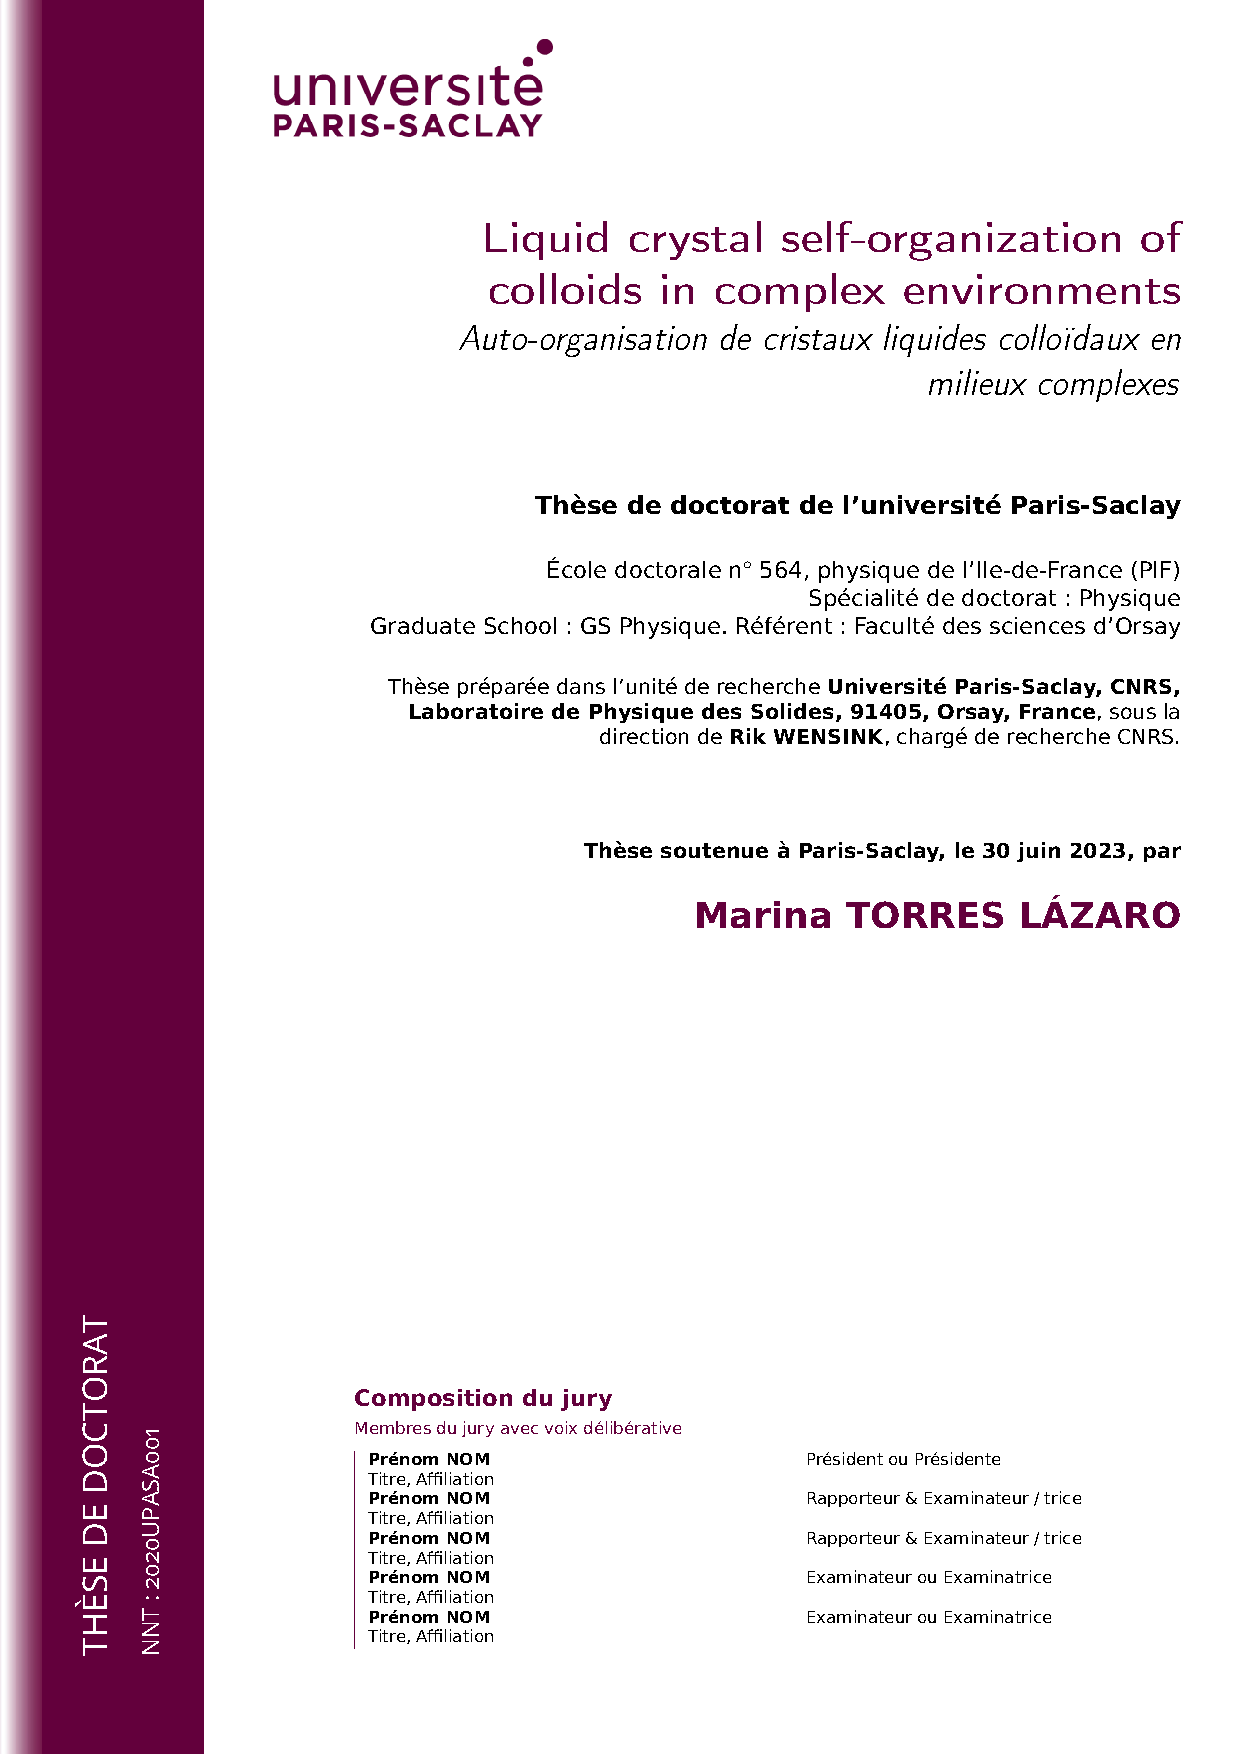
\includepdf[pages={1}]{coverpage/TORRES_coverpage.pdf}


\begin{dedication}
[content]
\end{dedication}





%%%%%%%%%%%%%%%%%%%%%%%%%%%%%%%%%%%%%%%%%%
% abstract && acknowledgments && contents && figures && tables
%%%%%%%%%%%%%%%%%%%%%%%%%%%%%%%%%%%%%%%%%%
\frontmatter
\setcounter{page}{1}
\pagenumbering{roman}



\chapter{Résumé}

Les systèmes en matière molle présentent, dans la plupart des cas, des échelles de longueur structurelle allant du nanomètre au micromètre, et sont donc placés dans le domaine de la "nanotechnologie". Les systèmes colloïdaux sont des exemples bien connus dans lesquels cette caractéristique est essentielle pour définir la plage dans laquelle un type de comportement très spécifique se produit. Les colloïdes sont des substances supramoléculaires et submicroniques dispersées dans un milieu qui peut être un liquide ou un gaz. Ils sont beaucoup plus gros que les molécules et, par conséquent, le milieu d'une suspension colloïdale peut souvent être considéré comme un "arrière-plan" en ce qui concerne la gamme de tailles des colloïdes : ce milieu peut être approximé comme un continuum. En même temps, les colloïdes sont suffisamment petits pour présenter un mouvement thermique considérable par rapport à l'effet de sédimentation (qui est causé par des forces gravitationnelles qui deviendraient plus importantes pour des particules de taille plus élevée). Les colloïdes ont été découverts pour la première fois par Perrin, qui a détecté le mouvement brownien comme une manifestation visible du mouvement thermique dans les dispersions de colloïdes de résine dans l'eau \cite{perrin1913atomes}.

Lorsque les particules colloïdales présentent des formes anisotropes, elles peuvent se trouver dans des phases cristallines liquides. Les cristaux liquides sont des substances qui ont l'apparence d'un liquide mais qui possèdent certains niveaux d'arrangement moléculaire semblables à des cristaux. Les cristaux liquides ont été découverts pour la première fois en 1888 par Friedrich Reinitzer, qui a remarqué qu'une substance à base de cholestérol avait deux points de fusion à des températures différentes, chacun d'eux donnant lieu à une phase liquide aux propriétés optiques différentes \cite{reinitzer1888beitrage}. À l'époque de Reinitzer, seules trois phases étaient connues (gaz, liquide et solide). Au fil des ans, on a découvert qu'un grand nombre de substances présentaient de nombreux états de la matière, y compris des phases cristallines liquides qui sont aujourd'hui largement utilisées dans les avancées technologiques telles que les écrans et les thermomètres à cristal liquide \cite{Li_2012}.

La principale différence entre un cristal liquide et les états gazeux, liquide et solide couramment observés est que les propriétés du premier sont anisotropes et varient en fonction de la direction, même si la substance elle-même reste fluide. Ces propriétés uniques sont dues à la forme allongée de ses éléments constitutifs, qui favorisent l'alignement collectif dans une certaine direction. En d'autres termes, les phases cristallines liquides sont des états supplémentaires de la matière, intermédiaires entre le gaz dilué et le solide cristallin, dont l'existence est liée aux degrés de liberté supplémentaires que possèdent les particules anisométriques par rapport aux particules sphériques.


Parmi les nombreuses phases cristallines liquides, on peut trouver différents degrés d'ordre, mis en évidence par exemple par la diffraction des rayons X et de la lumière. Les mesures de ce type permettent de classer ces systèmes en fonction de leur similitude avec la phase gazeuse ou la phase solide. Considérons, entre autres, les phases cristallines liquides suivantes, représentées dans \fig{frenchfig} :

La phase fluide {\em isotrope} (I) est très similaire aux phases gazeuse et liquide pour les particules sphériques et se caractérise par une absence totale d'ordre positionnel et orientationnel. Au stade immédiatement suivant, nous trouvons la phase {\em nématique} (N), dans laquelle les particules sont réparties de manière homogène sans ordre de position comme dans une phase liquide, mais sont ordonnées dans leur orientation suivant une direction moyenne : le directeur nématique $\bn$. Comme nous le voyons à plusieurs reprises tout au long de cette thèse, on peut trouver dans la nature des particules qui, en plus d'être anisotropes, présentent des caractéristiques chirales. Cela peut être dû à l'arrangement des atomes dans un composé moléculaire, à une forme de particule (hélicoïdale) dans certains systèmes colloïdaux ou à une distribution chirale des charges à la surface des particules, observée par exemple dans  les bâtonnets viraux filamenteux {\em fd} \cite{Gibaud_2017}. Lorsque les particules chirales sont en phase nématique, elles s'organisent en une structure fortement torsadée. Ce cas particulier de phase nématique est souvent appelé {\em cholestérique}.

La phase {\em smectique} (Sm) est plus proche de la phase solide. Dans les cristaux liquides smectiques, les particules sont ordonnées en couches et ne peuvent pas se déplacer librement entre elles. La phase smectique est à son tour divisée en plusieurs sous-phases aux propriétés légèrement différentes. Par exemple, la phase smectique A (SmA), où les particules peuvent se déplacer librement à l'intérieur des couches comme dans un liquide bidimensionnel, ou la phase smectique B (SmB), où il existe un ordre positionnel à long terme : à des concentrations plus élevées ou à des températures plus basses, les molécules ont tendance à s'arranger de manière à ressembler davantage à un réseau cristallin.

Une sous-classification des matériaux cristallins liquides est basée sur le mécanisme par lequel ils passent d'un état à l'autre. Les systèmes {\em thermotropes}, principalement formés par des constituants de faible poids moléculaire - et aussi certains polymères -, subissent des transitions de phase dues à des changements de température, puisque les propriétés thermodynamiques de ces espèces dépendent des forces d'attraction entre les molécules. Dans cette thèse, nous nous concentrons principalement sur les cristaux liquides {\em lyotropes}, qui se forment en augmentant la concentration des particules de soluté. C'est le cas des systèmes formés par des nanoparticules synthétiques et biologiques de haut poids moléculaire \cite{sonin1998inorganic,dogic-fraden_fil}, des polymères tels que l'ADN \cite{livolantDNAoverview} ou des surfactants dans un solvant \cite{fontell1981}. Le premier cas est celui étudié dans cette thèse, où le fait que la forme ne soit pas sujette à des fluctuations dues à des changements dans la composition du solvant est une simplification avantageuse par rapport à ses homologues amphiphiles et polymèriques.

Les premiers rapports expérimentaux sur les cristaux liquides lyotropes à base de nanoparticules remontent à la description du comportement cristallin liquide du virus de la mosaïque du tabac et de la tomate (TMV) \cite{Bawden,Bernal} et du pentoxyde de vanadium (V$_{2}$O$_{5}$) \cite{Zocher} au début du 20e siècle. Outre ces systèmes de particules en forme de bâtonnets, on a découvert que les particules colloïdales chargées en forme de plaques et les particules d'argile présentaient un comportement cristallin liquide \cite{Langmuir}. Actuellement, il existe de nombreux autres exemples de cristaux liquides lyotropes dans une grande variété de dispersions de particules colloïdales (principalement en forme de bâtonnets) et de solutions de polymères rigides (voir par exemple \cite{Dierking2020} pour une vue d'ensemble).

\begin{figure}
\includegraphics[width= \columnwidth]{figures/chapter-1/phases}
\caption[Exemples de cristaux liquides basiques formés par des molécules ou des nanoparticules en forme de bâtonnets]{ \label{frenchfig} (a)-(d) Exemples de cristaux liquides de base formés par des molécules ou des nanoparticules en forme de bâtonnets. (e) Les cristaux liquides peuvent être formés par des constituant chiraux; (f) ces particules génèrent un type particulier de phase nématique : le nématique chiral. Les implications de la chiralité moléculaire sur la mésostructure hélicoïdale (en particulier, le {\em pitch} mésoscopique) des phases nématiques chirales restent une question difficile.}
\end{figure}

Ce travail de recherche se concentre sur les approches théoriques et numériques pour l'exploration du comportement de phase dans les composés colloïdaux anisotropes, avec un intérêt particulier pour la transition de phase isotrope-nématique {\em entropique}. Cette transition est bien décrite par la théorie d'Onsager, proposée en 1949, qui suppose une similarité entre un gaz et une solution de particules \cite{onsager1949} ; et sera utilisée à plusieurs reprises dans ce manuscrit (plus particulièrement dans les chapitres \ref{disc_polymer} et \ref{hybridLC2}) avec d'autres outils théoriques et numériques pour étudier l'auto-organisation liquide-cristalline de bâtonnets ou de plaquettes colloïdales dans des environnements complexes. Grâce à nos recherches, nous espérons mieux comprendre le comportement de ce type de systèmes et contribuer au domaine plus large de la recherche sur les cristaux liquides.


%L'objectif central de cette thèse est d'étudier théoriquement l'auto-organisation des particules colloïdales de cristaux liquides (LC) avec différentes formes dans divers contextes. Beaucoup des études qui seront décrites dans le reste de cette thèse ont été inspirées par des travaux expérimentaux récents sur des systèmes de colloïdes avec des formes et des interactions bien contrôlées. En particulier, nous mentionnons les travaux expérimentaux de \cite{Grelet2014} sur le comportement de phase et la fonctionnalisation de fluides complexes de bactériophages filamentaires (fd et M13) qui présentent de nombreux phénomènes intéressants laissés ouverts à l'interprétation théorique ; ainsi que les résultats expérimentaux récents \cite{senyuk2021nematoelasticity,mundoor2021} sur la dispersion colloïdale de particules hautement anisotropes immergées dans des hôtes de cristaux liquides moléculaires. Un de nos objectifs principaux dans ce travail est de rendre compte de ces observations expérimentales en construisant des modèles simples mais réalistes pour les systèmes colloïdaux étudiés et en examinant les aspects pertinents de leur comportement de phase.

Le chapitre \ref{introduction} de cette thèse fournit une introduction au contexte et à la portée de la recherche présentée. Il couvre le contexte statistique mécanique, en particulier pour les fluides de particules anisométriques dures. Nous discutons ensuite de l'utilisation des simulations de Monte Carlo de particules dures, en mettant en évidence certaines particularités de telles simulations pour le cas de particules anisométriques. Dans l'ensemble, le chapitre sert de fondement pour le reste de la thèse, en exposant les concepts et les méthodes pertinents pour la recherche présentée dans les chapitres suivants.

Dans le chapitre \ref{disc_polymer}, un modèle théorique est proposé pour explorer le comportement de phase à faible concentration d'un système composé de batônnets faiblement flexibles liés de manière non covalente et traités comme des {\em living polymers} mélangés à des disques colloïdaux rigides non adsorbants. En utilisant une théorie du second viriel qui corrèle les différentes entropies associées aux polymères et aux disques, nous démontrons que de faibles fractions d'additifs discotiques favorisent la formation d'une phase nématoïde de polymère. À des concentrations plus élevées de disques, cependant, la phase est perturbée par l'alignement collectif des disques en faveur d'un fluide nématoïde discotique dans lequel les polymères sont dispersés de manière {\em antinématoïde}. Nous montrons que l'arrangement antinématoïde des polymères génère une distribution de poids moléculaires non exponentielle et stimule la formation d'espèces oligomériques. À des concentrations suffisantes, les disques facilitent une séparation de phase liquide-liquide qui peut être mise en coexistence simultanée avec les deux phases nématiques fractionnées, fournissant ainsi des preuves d'une coexistence à quatre fluides dans une mélange de cœurs durs de formes différentes sans forces interparticulaires cohésives. Nous stipulons les conditions dans lesquelles un tel phénomène pourrait être observé en expérimentation.

Les chapitres \ref{hybridLC1} et \ref{hybridLC2} abordent des problèmes liés aux cristaux liquides nématiques moléculaires hybrides. Dans cette partie du travail, nous considérons un système dans lequel les cristaux liquides cholestériques moléculaires sont dopés avec de fines particules colloïdales ayant de grands rapports longueur-largeur. Dans le chapitre \ref{hybridLC1}, nous considérons des insertions individuelles de colloïdes. Nous démontrons que les tiges ont une forte tendance à s'orienter perpendiculairement à l'axe hélicoïdal et au directeur local, conférant ainsi une forte biaxialité locale à la structure cholestérique hybride. Nous argumentons théoriquement que l'anisotropie élastique et l'étalement  de la courbure joue un rôle clé dans la stabilisation de l'ordre orthorhombique local le long de l'hélice. Nos prévisions sont corroborées par des résultats expérimentaux obtenus dans le groupe de I. Smalyukh (Université du Colorado, États-Unis) que nous examinons brièvement. Nous discutons également le cas des disques et trouvons un scénario similaire d'ordre biaxial anormal le long du directeur hélicoïdal pour les disques à ancrage homéotrope immergés dans des hôtes cholestériques à pas court.

Dans le chapitre \ref{hybridLC2}, nous utilisons la théorie d'Onsager pour rendre compte des effets collectifs dans le cas hypothétique où plusieurs particules colloïdales sont insérées dans le LC hybride. Ce cadre nous permet d'explorer des concentrations de colloïdes qui ne sont plus infiniment petites. Les corrélations entre les colloïdes entraînent des contributions élastiques et entropiques supplémentaires qui interfèrent avec les effets d'ancrage de surface explorés dans le chapitre précédent. Nous considérons deux régimes distincts, à savoir le couplage faible où l'ancrage de surface n'a qu'un impact marginal sur les orientations des colloïdes et le couplage fort où l'énergie de réalignement typique dépasse largement l'énergie thermique. Nous démontrons au couplage faible que les effets collectifs colloïdaux induits par l'interaction stérique colloïde-colloïde peuvent conduire à une séparation de phase liquide-liquide entre deux phases fluides biaxes. Dans le régime de couplage fort, nous soutenons que la force élastique peut faciliter la formation d'états bi-hélicoïdaux où l'organisation hélicoïdale des composants colloïdaux et moléculaires est inégale en pas et même en chiralité.

Finalement, dans le chapitre \ref{twistedrods}, nous utilisons des simulations de Monte Carlo approfondies, complétées par la théorie, pour explorer deux formes de gouttelettes importantes dans la littérature, à savoir la membrane torsadée et le ruban colloïdaux. Dans l'expérience, la structure de ruban allongée est trouvée à dominer à une force chirale élevée. Cependant, dans nos simulations, nous démontrons qu'en augmentant la chiralité, les membranes ont tendance à se transformer en structures à plusieurs domaines composées de plusieurs unités presque circulaires torsadées séparées par des parois $\pi$, tandis que la transition en rubans torsadés est entravée par la forte tension de surface subie par la gouttelette. Nous complétons nos simulations avec des descriptions théoriques microscopiques simples pour les deux morphologies de gouttelettes, ce qui nous permet de prédire l'évolution de l'angle de torsion à travers les membranes. Pour les rubans, notre théorie simple fournit des prévisions génériques pour la largeur de ruban typique, la torsion interne et l'angle d'inclinaison des bords qui sont en accord avec les observations expérimentales de rubans torsadés composés de tiges de virus {\em fd} mélangées avec du dextran.

{\large\textbf{Mots clés:}} cristal liquide; colloïde; théorie d'Onsager; Hard Particle Monte Carlo


\chapter{Summary}



Write abstract here.

{\large\textbf{Key Words:}} Template; Rice; USTC

\chapter{Acknowledgements}


Write acknowledgments here.

\tableofcontents

\listoffigures
\addcontentsline{toc}{chapter}{List of Figures}

% TO DO:
%\addcontentsline{toc}{chapter}{List of Symbols}




%%%%%%%%%%%%%%%%%%%%%%%%%%%%%%%%%%%%%%%%%%
% chapters
%%%%%%%%%%%%%%%%%%%%%%%%%%%%%%%%%%%%%%%%%%
\mainmatter
\setcounter{page}{1}
\pagenumbering{arabic}


\chapter{General introduction}

\begin{abstract}
  \blue{
  In this Chapter we introduce the concept of lyotropic liquid crystals, both from a practical and statistical mechanical point of view.  We also establish the aim of this thesis in relation to recent experimental work on colloidal mixtures.
  }

\end{abstract}


\section{Phenomenological background}

{\em Soft matter} is a term used to describe materials that are distinct from gases and solids, usually excluding simple fluids. A wide range of systems, including soap bubbles, gels, elastomers, liquid crystals, or biological fluids, can be categorized as soft matter. Defining the boundaries of such a vast domain can be challenging due to the diverse topics and segregated nature of researchers, which come from a number of distinct disciplines. Nevertheless, a clear community with a common language exists, and major research topics can be identified that encompass most current studies in this field \cite{borsali2018soft}.

Soft matter systems exhibit, in most cases, structural length scales ranging from a nanometer up to a micrometer, and thus are placed within the domain of ‘nanotechnology’. Colloidal systems are well known examples in which this feature is essential to define the range where a very specific type of behavior occurs. Colloids are supramolecular submicron sized substances dispersed in a medium that can be a liquid or a gas. They are much bigger than normal molecules, and hence the medium in a colloidal suspension can often be regarded as ‘background’ with respect to the colloidal size range: this medium may be approximated as a continuum. At the same time, colloids are small enough to present considerable thermal motion in comparison to sedimentation (which is caused by gravitational forces that would become more important for higher-sized particles). Colloids were first discovered by Perrin, who detected Brownian motion as visible manifestation of thermal motion in dispersions of resin colloids in water \cite{perrin1913atomes}.

When colloidal particles have anisotropic shapes, they can present liquid crystalline phase behaviors. Liquid crystals are substances that have the appearance of a liquid but possess certain levels of molecular arrangement similar to crystals. Liquid crystals were first discovered in 1888 by Reinitzer, who noticed that a cholesterol-based substance had two melting points at different temperatures, each of them giving way to a liquid-like phase with different optical properties \cite{reinitzer1888beitrage}. At the early time of Reinitzer only three phases wew known (gas, liquid and solid). Over the years, a big number of substances have been discovered to exhibit many states of matter, including liquid crystals that are now widely used in technological advancements such as liquid crystal screens and thermometers \cite{Li_2012}.

The key difference between a liquid crystal and the commonly observed gas, liquid and solid states is that properties in the first one are anisotropic and vary with direction, even though the substance itself remains fluid. These unique properties emerge due to the elongated shape of its building blocks, which promote collective alignment along a certain direction. In other words, liquid crystalline phases are additional states of matter which are intermediate between the dilute gas and the crystalline solid, and whose existence is related to the additional {\em orientational} degrees of freedom anisometric particles have compared to spherical ones.

Among the numerous liquid crystalline phases, different degrees of order can be found, evidenced for instance by diffraction of X-rays and light. Measurements of this kind provide a frame to classify these systems by its similarity to either the gas or the solid phase. Let us consider, as an example, the following liquid crystalline phases:

The {\em isotropic} (I) fluid phase is very similar to the gas and liquid phases for spherical particles and is characterized by a complete absence of positional and orientational order. At the inmediately next stage, we find the {\em nematic} (N) phase, in which particles are homogeneously distributed without positional order as in a liquid phase, but are ordered in their orientation following an average direction: the {\em nematic director} $\bn$. As it will be repeatedly discussed throughout this thesis, in nature one can find particles that, in addition to being anisotropic, present chiral features. This can be due to the arrangement of atoms in a molecular compound, to a (helicoidal) particle shape in some colloidal systems or to a chiral distribution of charges at the surface of the particles, observed for instance in filamentous bacteriophages viral rods named fd \cite{Gibaud_2017}. When these particles are in nematic phase, they arrange themselves into a strongly twisted structure. This special case of a nematic phase is often called {\em cholesteric}.

The {\em smectic} (Sm) phase is closer to the solid phase. In smectic liquid crystals, particles are ordered in layers and cannot move freely between them. The smectic phase is, in turn, divided into several sub-phases with slightly different properties. Examples are the smectic A phase (SmA), where particles can move freely inside the layers as in a two-dimensional liquid; or the smectic B phase (SmB), where there is long-ranged positional order: at higher concentrations or lower temperatures, molecules tend to arrange themselves into something more similar to a crystalline lattice.

One sub-classification of liquid crystal materials is based on the mechanism by which they transition from one state to another. {\em Thermotropic} systems, mainly constituted by low molecular weight constituents -and also some polymers-, undergo phase transitions due to changes in temperature, while {\em lyotropic} liquid crystals form upon increasing the concentration of solute particles. This is the case of systems formed by high-molecular weight colloidal particles, polymers or surfactants in a solvent. In this thesis, we focus on lyotropic liquid crystals, specifically those composed of viral fd rods as the fundamental building block. Filamentous viruses are a well-studied model system for elongated colloidal particles due to their regular shape and size, high abundance, and the possibility to genetically and chemically modify their surface.

This research work focuses on both theoretical and numerical approaches for the exploration of phase behavior in anisotropic colloidal compounds, with a particular interest in the {\em entropic} isotropic-nematic phase transition. This transition is well described by Onsager's theory, proposed in 1949, which assumes a similarity between a gas and a particle solution \cite{onsager1949}; and will be used repeatedly throughout the following chapters along with other theoretical tools to study the liquid-crystalline self-organization of colloidal rods or platelets in complex environments. Through our research, we hope to gain a better understanding of the behavior of this kind of systems and contribute to the broader field of liquid crystal research.

\blue{

\section{Phenomenological background}


It is  well-known from everyday experience that, under certain conditions, matter can transform from one state to the other
by a {\em phase transition}. For instance, increasing the temperature may lead to
boiling and evaporation of water or the melting of ice, nitrogen gas can be liquefied
at low temperatures and high pressures.
As to the liquid crystals we discuss here,  phase transitions among the different
states may be brought about
in two different ways; one by varying the temperature  and the other by changing
the concentration of particles in solution. The variety of systems characterized by the former
is qualified as `thermotropic' and consists mainly of systems of anisometric low molecular weight constituents (and also certain polymers).
In this thesis we shall however restrict ourselves to the latter class of systems; the {\em lyotropic}
liquid crystals. These are composed of high-molecular weight colloidal particles, polymers
or surfactants in a solvent such that the formation of these liquid crystals occurs upon increasing the {\em concentration} of the solute particles.

Historically, lyotropic liquid crystals were first recognised in the 1920s by Zocher \cite{Zocher}
who investigated nematic textures in solutions of rodlike inorganic vanadiumpentoxide (V$_{2}$O$_{5}$) particles.
Later, similar observations were reported by Langmuir \cite{Langmuir} for clay platelets
and Bawden {\em et al.} \cite{Bawden,Bernal} for Tobacco Mosaic Virus (TMV) rods.
At present, there are many other examples of lyotropic liquid crystals to be found in a wide
variety of dispersions of (mainly rodlike) colloidal particles and solutions of stiff polymers
(see e.g. Refs. \cite{Vroege92,Gabrieloverzicht} for an overview).
In the last decade much of the experimental effort in colloid science
was focussed on the development and characterization of colloidal {\em model systems} comprising particles
with a well-defined size and shape. The effective interactions between the particles can often be tailored
either by chemically altering the surface of the particles or by changing the solvent
conditions through variation of the ionic strength or the addition of non-adsorbing polymer.
As to anisometric colloids, two  important examples of these model systems are the  Boehmite  (AlOOH)  rods
\cite{Buiningwater,vanBruggen}
and the plate-shaped  Gibbsite (Al(OH$)_{3}$) particles \cite{Wierenga}.
These particles can be stabilised for instance by grafting a layer of polymer onto the particle surface
 \cite{vanBruggenPIB,vanderKooij}. If the particles are subsequently dispersed in a suitable solvent,
the polymer layer acts as a steric stabilizer which gives rise to short-ranged repulsive interactions,
closely resembling so-called {\em hard} interactions, i.e. the particles repel each other when they touch (they are
impenetrable) but do not interact otherwise.
Owing to their simple hard-body interactions the sterically stabilized systems
are particularly suitable for studying the influence of {\em particle shape}, explored by either
changing the intrinsic shape of the particles or by mixing particles with distinctly different sizes and shapes,
on the liquid crystalline phase behaviour of anisometric colloids \cite{felixthesis}.

\subsection{Entropic phase transitions}

On the theoretical side, the field of statistical mechanics of lyotropic
liquid crystals  was opened up by Lars Onsager in the 1940s. He recognized that the transition
from an isotropic to a nematic state in solutions containing sufficiently anisometric particles
can be described successfully  within a virial expansion of the free energy truncated after
the second virial term, an approach which could not be used to explain the gas-liquid transition for spherical particles.
 One of the crucial insights of Onsager was that the transition
can be explained by hard-body repulsions only, thereby dismissing the widespread notion
that attractive forces between particles  must be responsible for the formation of
 aligned configurations. The theory of Onsager will be described comprehensively in  Sec. 1.3.


About a decade after Onsager's work, Alder, Wainwright and others \cite{ALDER57,WOOD57} first showed by means of computer simulations that
a similar disorder-order transition, albeit of the positional degrees of freedom, occurs in a fluid of hard spheres. Subsequent work by
Hoover and Ree \cite{HooverRee} established that if the hard-sphere packing fraction
exceeds $\phi=0.494$ a fluid  spontaneously freezes into a crystalline
solid phase with a packing fraction $\phi=0.545$.
Much later, computer simulations by Frenkel {\em et al.}  revealed the stability
of smectic and columnar liquid crystals which appear upon densifying systems of respectively hard rods \cite{Frenkel88} and
 hard platelets \cite{FrenkelLiqcryst,Veerman},  without  attractive interactions between the particles.
The transitions of matter mentioned here share an important characteristic; they are driven purely by {\em entropy}, i.e. there are no energetic effects involved.
For this reason these ordering phenomena are nowadays
often referred to as {\em entropic phase transitions} \cite{Frenkelsoft}.
The notion that spontaneous ordering
of particles corresponds to an increase of the total entropy  may seem counter-intuitive
at first sight, since an increase  of order is usually connected to a decrease of entropy.
Yet, the general mechanism behind these transitions can be understood as follows.
Although the particles lose entropy because the density --in terms of orientations or positions--
is no longer uniform, this loss is more than offset by the simultaneous gain of translational
entropy, i.e.  the available space per particle increases as the particles align or freeze into
a crystal lattice.

\subsection{Mixtures}

So far we have implicitly assumed that all particles which build up a gas, liquid (crystal) or solid phase
are identical. Many systems in nature are however {\em mixtures} containing a number of different types of
particles or molecules. In this respect we may roughly distinguish
between mixtures of chemically distinct moieties on the one hand and so-called {\em polydisperse} mixtures on
the other. Examples of the first are blood
(containing red and white blood cells, plasma etcetera),
mayonnaise (a mixture of oil and vinegar) and milk (consisting of dispersed fat globules, casein micelles and
whey proteins).
Polydisperse mixtures are characterized by a large (potentially infinite) number of
species --all belonging to a {\em single} family of particles-- with  continuously varying properties such as particle shape, size or possible surface charge.
Common examples of these are colloidal model systems , where the particles usually have the same
basic shape (e.g.  spheres, rods or plates) but  a {\em range} of
radii, lengths, diameters, etcetera. Of course, in reality many systems
share characteristics of both classes; they
may comprise a number of distinct species  each with some degree of polydispersity with respect to
one or more properties of the particle family.

It is not surprising that the phase behaviour of  mixtures is richer than that of pure systems
--if only for the additional {\em entropy of mixing}-- and
that mixing different species may lead to  phenomena not encountered in one-component systems.
In particular, depending on the miscibility of the species involved,  mixing
may sometimes lead to a destabilization of a homogeneous state
causing a phase separation into two or more phases, each with a different
density and/or composition. The associated segregation of species among the coexisting phases,
called  {\em fractionation}, is inherent to mixtures and may sometimes give rise to surprising phenomena,
as shown in the next Chapter.
Mixing particles with distinctly different sizes or shapes
may also cause the formation of ``new" phases whose structures are not observed in pure systems
of the constituent species. For instance, in a two-component (or binary) mixture
 of rod- and platelike colloids we may encounter the so-called {\em biaxial} nematic
phase, in which both particles types are aligned
in mutually perpendicular directions. Similarly, mixing spheres of two (or more) different sizes
may give rise to the formation of various solid states with intricate
lattices structure  not encountered in pure solids \cite{Bartlettbinary}.


\section{Scope of this thesis}
The central aim of this thesis is to theoretically investigate
the effects of  {\em mixing}  particles with different shapes
on their liquid crystal phase behaviour.
Many of the studies to be described in the remainder of this thesis have been triggered off
by recent experimental observations in mixtures of colloids with well-controlled shapes
and interactions.
In particular, we mention the experimental work of Van der Kooij \cite{felixthesis} who investigated a vast number
of mixtures which display many interesting phenomena left open for theoretical interpretation.
One of our primary goals in this work is to account for these
experimental observations by constructing simple, yet realistic,  models
for the colloidal systems under consideration
and by scrutinizing relevant aspects of their phase behaviour.

The first part of this thesis will be devoted to binary mixtures of anisometric particles.
In Chapter 2 a simple model is proposed that allows to qualitatively explain
the recently observed isotropic-nematic density inversion in polydisperse systems of colloidal platelets.
In the next two chapters  we shall be concerned with mixtures of rods and platelets and
provide a theoretical underpinning for the low-concentration part of the experimental
phase diagram. We also assess the possible stability of the disputed biaxial nematic phase
in experimentally realizable mixtures.
In Chapter 5 we conclude the first part with  an overview on demixing transitions
within the isotropic and nematic phases of binary mixtures of particles
whose size differs only in one particle dimension. Previously published results for rodlike particles
will be combined with new results for platelets to compare phase diagram topologies and
demixing mechanisms pertaining to the various mixtures.

In the second part of this thesis we address the more challenging issue of calculating
phase equilibria in polydisperse mixtures of anisometric particles.
In Chapter 6 we present a study of isotropic-nematic phase coexistence in systems of
length-polydisperse hard rods, focussing in particular on fractionation effects and
the possibility of a demixing of the nematic phase.
Chapter 7 deals with polydisperse systems of thickness-polydisperse
platelets. The binary model, introduced in Chapter 2, is extended to a polydisperse
one which allows us to provide a more realistic, albeit still qualitative, description of the experimental observations.
In Chapter 8 we provide a preliminary
calculation on the competition
between smectic and columnar ordering in systems of polydisperse hard rods.  As a first-order
approximation we consider an artificial model system of {\em perfectly aligned} cylinders. The  possibilities of extending the approach towards a more realistic one will be discussed.


The contents of  Chapter 9 of this thesis differ somewhat from the  rest because of the introduction of an  {\em external field}.
Inspired by recent experimental observations of a significant sedimentation in dispersions of platelets
 we illustrate the drastic effect of gravity
 on the phase behaviour of colloidal mixtures. As an example we consider a system
of sedimenting platelets mixed with non-sedimenting ideal polymers, as studied
experimentally by Van der Kooij. Also here,  the results of the calculations
reveal an improved description of the experimentally observed
behaviour.

Finally, in Chapter  10  we present a free-volume theory for a columnar state of hard platelets  by combining the traditional cell model with an appropriate fluid description which accounts for the rotational freedom of the particles in the (one-dimensional) direction of the phase. Excellent quantitative agreement is found with recent computer simulation results.



\section{Statistical mechanical background}
\noindent In this section we introduce the statistical mechanical framework
of  Onsager's second virial theory \cite{onsager1949,Vroege92,Cotter} to
describe the thermodynamic properties of a spatially homogeneous fluid of
hard colloidal rods or
platelets. The theory is then modified to account for
higher virial terms by means of a decoupling approximation as devised by Parsons \cite{Parsons}.
Finally, we introduce a bifurcation analysis to verify  the stability of the  fluid
with respect to the spatially {\em inhomogeneous} liquid crystalline states.

\subsection{Fluids of hard anisometric particles}
We start from an (imperfect) gas of $N$ identical cylindrically symmetric particles in a volume $V$.
Assuming a pairwise additive interaction potential we can express the total potential energy $U_{N}$  as a summation over pairs
\begin{equation}
U_{N}=\sum_{i<j} u(\bfr_{ij}; \Omega_{i}, \Omega_{j}),
\end{equation}
where $\bfr_{ij}=\bfr _{j}- \bfr _{i}$ is the vector connecting the centres of mass of particles $i$ and $j$;
$\Omega_{i}$ and $\Omega_{j}$ represent the solid angles describing the orientations of
the respective particles with respect to some space-fixed coordinate system.
For hard-core interactions the pair potential explicitly reads
\begin{equation}
u(\bfr_{ij}; \Omega_{i}, \Omega_{j}) =
\begin{cases}
\infty  &\text{if $i$ and $j$ overlap;} \\
0 &\text{otherwise.} \label{0pairpot}
\end{cases}
\end{equation}
The  description can be applied analogously to dispersions of colloidal particles
 but the direct pair potential $u$
 should then be replaced by the potential of mean force $w(\bfr_{ij};\Omega_{i},\Omega_{j})$ describing
the interaction between the  particles $i$ and $j$
dispersed in a  solvent with a fixed chemical potential \cite{macmillan,Hill}.
This procedure involves a configurational average of the solvent molecules accounting for
their mutual interactions and the interactions with the dispersed particles.

The configurational partition function $Q_{N}$ for the system reads
\begin{equation}
Q_{N}=\frac{1}{\mathcal{V} ^{N} N!}\int d\bfr^{N}\int d\Omega ^{N}\exp\left[-\beta U_{N}(\bfr^{N}; \Omega^{N})\right],
\label{0qdef}
\end{equation}
with $\beta= 1/k_{B}T$ and $\mathcal{V}$ the (de Broglie) thermal volume, arising from
integrations over the translational and rotational momenta of the anisometric particles.
The positional and orientational degrees of freedom of the particles are collectively denoted by
$\{\bfr^{N};\Omega^{N}\}$.
If we assume that there are no  {\em a priori} restrictions on the particle orientations
we may approximate the  angular integrations  to arbitrary accuracy by dividing
the orientational phase space, i.e. the surface of a unit sphere, into $s$
arbitrarily small equal sections  with a surface $\Delta \Omega = 4\pi/s$ and summing over all
possible orientation distributions $\{N_{1},N_{2}, \ldots, N_{s}\}$, where $N_{k}$ is the
number of particles with its solid angle $\Omega$ in the $k$-th section centered about
$\Omega_{k}$ such that
\begin{equation}
\sum _{k=1}^{s} N_{k} =N. \label{0behoud}
\end{equation}
The partition function Eq. (\ref{0qdef}) then becomes
\begin{align}
Q_{N}=&\frac{1}{\mathcal{V} ^{N} N!}\left(\frac{\Delta \Omega}{4\pi}\right)^{N}
\sum_{N_{1}=0}^{N}\ldots \sum_{N_{s}=0}^{N}\frac{N!}{\prod_{k=1}^{s}N_{k}!} \nonumber \\
&\times\int d\bfr^{N}
\exp\left[-\beta U_{N}(\bfr^{N}; N_{1},N_{2},\ldots,N_{s})\right], \label{0Qalgemeen}
\end{align}
where the summations need to be carried out under the condition of Eq. (\ref{0behoud}).
For large $N$ it is justified to replace the sum  by its maximum term \cite{Hill}.
Denoting the set (i.e. orientation distribution) which maximizes $\ln Q_{N}$ (and hence $Q_{N}$) by
 $\{\tilde{N}_{1},\tilde{N}_{2},\ldots,\tilde{N}_{s}\}$ we obtain
\begin{equation}
Q_{N}\approx \frac{1}{\mathcal{V} ^{N} N!}\left(\frac{\Delta \Omega}{4\pi}\right)^{N}
\frac{N!}{\prod_{k=1}^{s}\tilde{N}_{k}!}\int d\bfr^{N}
\exp\left[-\beta U_{N}(\bfr^{N}; \tilde{N}_{1},\tilde{N}_{2},\ldots,\tilde{N}_{s})\right].
\end{equation}
The partition function can be expressed in a more convenient form after some rearranging. This yields
\begin{equation}
Q_{N}= \underbrace{\frac{V^{N}}{\mathcal{V} ^{N} N!}}_{Q_{N}^{\text{trans}}}
\underbrace{\left(\frac{\Delta \Omega}{4\pi}\right)^{N}
\frac{N!}{\prod_{k=1}^{s}\tilde{N}_{k}!}}_{Q_{N}^{\text{orient}}}
\underbrace{\left < \exp\left[-\sum_{i<j}\beta w(\bfr_{ij};
\tilde{N}_{i},\tilde{N}_{j})\right] \right >_{\{\tilde{N}_{1},\tilde{N}_{2},\ldots,\tilde{N}_{s}\}}
}_{Q_{N}^{\text{int}}},
\end{equation}
where the brackets denote a (normalized) configurational average over all positional and orientational
coordinates under the condition that the particles obey an orientational distribution
according to the set $\{\tilde{N}_{1},\tilde{N}_{2},\ldots,\tilde{N}_{s}\}$.
The first terms $Q_{N}^{\text{trans}}$ and $Q_{N}^{\text{orient}}$ are  identified as the translational (ideal gas) and
orientational contributions, respectively, whereas the bracketed one accounts for the hard-body interactions between
the particles.
The Helmholtz free energy is obtained from the standard relation $\beta F= -\ln Q_{N}$.
Applying this to $Q_{N}^{\text{trans}}$ gives the common ideal free energy
$\beta F_{\text{id}}= N\left[\ln (\rho \mathcal{V})-1\right]$, with $\rho=N/V$ the number density.
For the orientational part we obtain
\begin{equation}
\beta F_{\text{orient}}=N\left\{\ln \left[\frac{4\pi}{\Delta \Omega}\right] + \sum_{k=1}^{s}\tilde{n}_{k}\ln \tilde{n}_{k} \right\},
\label{0fordiscreet}
\end{equation}
in terms of the number fractions $\tilde{n}_{k}=\tilde{N}_{k}/N$ with $\sum_{k=1}^{s}\tilde{n}_{k}=1$.
Introducing the normalized {\em orientational distribution function} (ODF) $f(\Omega_{k})$ we may
write $\tilde{n}_{k}=f(\Omega_{k})\Delta\Omega$. Using this in Eq. (\ref{0fordiscreet}) and
taking the  limit $\Delta \Omega \rightarrow 0$ for a {\em continuous} distribution in $\Omega$ we
obtain the following expression for the orientational free  energy
\begin{equation}
\frac{\beta F_{\text{orient}}}{N}=\int f(\Omega)\ln \left[4\pi f(\Omega)\right]d\Omega.
\label{0forient}
\end{equation}
The configurational partition function  $Q_{N}^{\text{int}}$ can be approximated
systematically by a {\em virial expansion} in terms of the density variable $\rho$ \cite{hansenmacdonald}.
At low densities it is justified to make a second virial approximation   by taking each of the $N(N-1)/2$ pair interactions independent from all others
so that
\begin{align}
Q_{N}^{\text{int}}&= \left \langle \prod _{i<j}
\exp\left[-\beta w(\bfr _{ij}; \Omega_{i}, \Omega_{j})\right]  \right \rangle _{f}
\approx \prod _{i<j}
\left < \exp\left[-\beta w(\bfr _{ij}; \Omega_{i}, \Omega_{j})\right]  \right>_{f} \nonumber \\
&\approx\left<1+\Phi_{12}\right>_{f} ^{N(N-1)/2}. \label{0secondvir}
\end{align}
The subscript $f$ indicates the condition that the orientational distribution is given by
$f(\Omega)$. Furthermore, $\Phi_{12}$ is the Mayer function, defined as
\begin{equation}
\Phi_{12}\equiv \exp\left[-\beta w(\bfr _{12}; \Omega_{1}, \Omega_{2})\right]-1.
\end{equation}
Applying the hard-core pair potential Eq. (\ref{0pairpot}) we see that this function is equal to -1  if
two particles $1$ and $2$ overlap and zero otherwise.
Spatially integrating the Mayer function
yields the so-called pair cluster integral $\beta _{1}$:
\begin{equation}
\beta_{1}(\Omega_{1},\Omega_{2})\equiv \frac{1}{V} \int d\bfr_{1}d \bfr_{2} \Phi(\bfr _{12}; \Omega_{1}, \Omega_{2})=-v_{\text{excl}}(\Omega_{1},\Omega_{2}),
\label{0cluster}
\end{equation}
which is equal to minus the {\em excluded volume} $v_{\text{excl}}$ of two anisometric particles at fixed
solid angles $\Omega_{1}$ and $\Omega_{2}$.
Using this in Eq. (\ref{0secondvir}) yields
\begin{align}
Q_{N}^{\text{int}}&\approx \left[1-\frac{1}{V} \iint d\Omega_{1} d\Omega_{2}
f(\Omega_{1})f(\Omega_{2})v_{\text{excl}}(\Omega_{1},\Omega_{2})\right]^{N(N-1)/2} \nonumber \\
&\approx \exp\left[-N \frac{\rho}{2}  \iint d\Omega_{1} d\Omega_{2}
f(\Omega_{1})f(\Omega_{2})v_{\text{excl}}(\Omega_{1},\Omega_{2})  \right].
\end{align}
Collecting results we obtain the following expression for the free energy
of a fluid of hard anisometric particles in the second virial approximation:
\begin{align}
\frac{\beta F}{N} =& \beta \mu_{0}+\ln\left[\mathcal{V}\rho\right]-1+
\int f(\Omega)\ln \left[4\pi f(\Omega)\right]d\Omega \nonumber \\
&+\frac{\rho}{2} \iint d\Omega d\Omega^{\prime}
f(\Omega)f(\Omega^{\prime})v_{\text{excl}}(\Omega,\Omega^{\prime}). \label{0freetot}
\end{align}
with $\mu_{0}$ a reference chemical potential of the dispersed particles depending
only on the solvent conditions. Higher order contributions in the virial expansion of the free energy
--involving clusters of three, four, etcetera particles--
can be derived using similar arguments as in Eq. (\ref{0secondvir}) \cite{vankampen}.
In the {\em third virial} approximation for example we encounter the triplet cluster
integral $\beta_{2}(\Omega_{1},\Omega_{2},\Omega_{3})$
\begin{equation}
\beta_{2}(\Omega_{1},\Omega_{2},\Omega_{3})\equiv \frac{2}{V}\iiint
d\bfr_{1}d\bfr_{2}d\bfr_{3} \Phi_{12}\Phi_{13}\Phi_{23}, \label{0beta2}
\end{equation}
which is nonzero only if three particles overlap simultaneously.
Eq. (\ref{0beta2}) and higher order cluster integrals are notoriously difficult to calculate
because this requires knowledge of the excluded volume of a multi-particle
cluster as a function of the orientations of all particles involved.
In practice, other methods are adopted to include higher virial terms, albeit
approximately, such as
`scaled particle' \cite{Cotterspt,Cotter} and density functional theories (see \cite{Vroege92,DFTspecialJPCM} for a review).
In this thesis we shall often use the so-called decoupling approximation, to be described
in Sec. 1.3.3.


The next step is to minimize the free energy, at a given density $\rho$, with respect to
the non-conserved orientational degrees of freedom.
In practice, there are two different ways to find this minimum; a formal approach and
a trial function method which we both shall discuss briefly here.
 The formal way  is to apply a functional differentiation of the free energy
with respect to the ODF $f(\Omega)$. This yields the stationarity condition:
\begin{equation}
\frac{\delta}{\delta f(\Omega)} \left[\frac{\beta F}{N}-\lambda^{\prime} \int f(\Omega)d \Omega \right]=0,
\label{0statcond}
\end{equation}
where $\lambda^{\prime}$ is a Lagrange multiplier to be determined from the
normalization condition for the ODF:
\begin{equation}
\int f(\Omega)d\Omega =1.
\end{equation}
Inserting the free energy Eq. (\ref{0freetot}) gives a nonlinear integral equation
\begin{equation}
\ln[4\pi f(\Omega)]=\lambda - \rho \int f(\Omega^{\prime})v_{\text{excl}}(\Omega,\Omega^{\prime})
d\Omega^{\prime}, \label{0inteq}
\end{equation}
with $\lambda=\lambda^{\prime}-1$. A trivial solution to Eq. (\ref{0inteq}) is
the constant $f(\Omega)=1/4\pi$ describing an {\em isotropic} fluid in which
all particle orientations are equally probable.
The thermodynamic equilibrium ODF for a {\em nematic} state --which
will be a peaked function--
can however only be obtained
 numerically e.g. in terms of a series expansion in
Legendre polynomials \cite{kayser,lasher,lakatos} or by means of a discretization scheme \cite{herzfeldgrid}.
It is important to realize that for  {\em uniaxial} particles the ODF satisfies
both azimuthal symmetry around the nematic director and inversion symmetry.
The former implies that the ODF depends only on the  polar angle $\theta$
between the particle orientation vector and the nematic director\footnote{An exception to this case is a mixture of uniaxial rods and plates,
where the ODF may depend on the azimuthal angle as well
due to a possible {\em biaxial} symmetry of the nematic phase.
This will become clear in Chapter 4.}, so that $f(\Omega)=f(\theta)$.
The latter  implies the angles $\theta$ and $\pi-\theta$ being equivalent, thus $f(\theta)=f(\pi-\theta)$.



To avoid the necessity of solving the nonlinear integral equation Eq. (\ref{0inteq}) one may
choose the trial function approach instead. The ODF $f(\Omega)$ in Eq. (\ref{0freetot}) is then
replaced by a {\em fixed functional form}
depending on one or more variational parameters and the free energy is subsequently minimized
with respect to these parameters.
This approach was first employed by Onsager  in his original paper \cite{onsager1949} where he used the following
trial form:
\begin{equation}
f_{O}(\cos \theta) =\frac{\alpha \cosh (\alpha \cos\theta)}{4\pi\sinh \alpha},
\end{equation}
in terms of the variational parameter $\alpha$.
Although this trial function gives reasonable results for the isotropic-nematic
phase transition the analysis involved is
quite complicated.
In this thesis we shall therefore often use the simpler Gaussian trial ODF, introduced
by Odijk \cite{OdijkLekkerkerker}:
\begin{equation}
f_{G}(\theta ) \cong   \left\{
\begin{tabular}{lll}
$Z\exp [-\frac{1}{2}\alpha\theta ^{2}]$ & if & $%
0\leq \theta \leq \frac{\pi }{2}$ \\
&  &  \\
$Z\exp [-\frac{1}{2}\alpha (\pi -\theta )^{2}]$
& if & $\frac{\pi}{2}\leq \theta \leq \pi $%
\end{tabular}
\right.  \label{0ODF}
\end{equation}
The normalization constant $Z=Z(\alpha)$ can be calculated analytically
by means of an asymptotic expansion for large $\alpha$. Noting
that $f_{G}(\theta)$ is then a rapidly decaying function we may expand as follows
\begin{align}
Z&=\left[\int_{0}^{2\pi} d \phi \int _{0}^{\pi} \exp \left[-\frac{1}{2}\alpha\theta ^{2}\right] \sin\theta d\theta\right]^{-1}
\sim \left[ 4\pi \int _{0}^{\infty} \exp \left[-\frac{1}{2}\alpha\theta ^{2}\right]\left\{ \theta - \frac{1}{6} \theta ^{3}+\ldots \right \}
 d\theta  \right]^{-1} \nonumber \\
&\sim \frac{\alpha}{4\pi}\left(1+\frac{1}{3\alpha}+\ldots \right), \label{0norma}
\end{align}
where the error introduced by extending  the $\theta$-integration  to infinity is $\mathcal{O}
(\text{e}^{-\alpha})$. Retaining the leading order term in Eq. (\ref{0norma}) we see that
the Gaussian ODF, unlike $f_{O}(\cos\theta)$,
does {\em not} give the correct isotropic ODF $1/4\pi$ in the limit $\alpha \rightarrow 0$, since $f_{G}(\theta)$
vanishes in this limit. Using the Gaussian ODFs
we can calculate the {\em typical} or root-mean-square polar angle, which is related to the variational parameter
via $\langle\theta^{2}\rangle^{1/2}\propto  \alpha^{-1/2}$, showing that it
will be small for large $\alpha$. We shall  use this relation implicitly in Chapter 5
where  an alternative description of the trial function approximation will be presented
 entirely in terms of these typical angles.


A benefit of using the Gaussian trial ODF
is that it renders the Onsager theory analytically tractable.
The free energy minimization can be carried out entirely analytically,
which reveals that $\alpha\propto \rho^{2}$,
whereas approximate asymptotic expressions
can be derived for the orientational and
excess parts of the free energy Eq. (\ref{0freetot}) \cite{Vroege92,OdijkLekkerkerker}.
Although the Gaussian ODF
is {\em not} a solution of the the exact stationarity condition Eq. (\ref{0statcond})
it  does satisfy an exact high-density scaling relation for the
ODF, as was shown by Van Roij \cite{vanroijmulderscaling},
 owing to the abovementioned
quadratic density-dependence of the variational parameter.
This in turn implies that the Gaussian ODF is particularly suitable
for strongly ordered nematic phases.
As to  mixtures of rods with different lengths, the Gaussian ODF
has so far been successful in explaining the generic features of the isotropic-nematic
phase behaviour
such as a fractionation effect, a widening of biphasic gap \cite{OdijkLekkerkerker} and the
existence of triphasic and nematic-nematic equilibria \cite{LekkerVroeg}.





%In this section we present an analytical theory based on the approximate
%Gaussian trial orientation distribution function (ODF) as formulated by
%Odijk {\em et al.} \cite{OdijkLekkerkerker}, which is a simplified version of the
%trial ODF used by Onsager \cite{Onsager}.


%In this section we present an analytical theory based on the approximate
%Gaussian trial orientation distribution function (ODF) as formulated by
%Odijk {\em et al.} \cite{OdijkLekkerkerker}, which is a simplified version of the
%trial ODF used by Onsager \cite{Onsager}. For bidisperse systems of rods
%with different lengths, the Gaussian ODF successfully explained features
%like the fractionation effect, the widened biphasic gap \ \cite
%{OdijkLekkerkerker} and, somewhat later, the existence of triphasic and
%nematic-nematic equilibria \cite{LekkerVroeg}. A recent analysis by van Roij
%\cite{vanRoij96/2} based on elaborate numerical calculations of the exact
%high density ODF essentially confirmed all conclusions of  \cite
%{LekkerVroeg}, thus emphasizing the virtues of the Gaussian approximation.

As is clear from Eq. (\ref{0cluster}) the key ingredient in the Onsager theory is the excluded volume of two particles
which depends essentially on the shape of the particles under consideration.
In this thesis we shall model the particles as cylinders with length $L$ and $D$;
slender rods are then characterized by  $L/D\gg 1$ whereas thin platelets
have $L/D\ll 1$. Henceforth, we will use the
ratio of the largest to the shortest dimension of the particle, the {\em aspect ratio}, to quantify the anisometry of the particle.
The general expression for the excluded volume of
two different cylinders with lengths $L_{1}$ and $L_{2}$ and diameters $D_{1}$ and $D_{2}$ at mutual angle
$\gamma$ has been derived
in closed form by Onsager in a remarkable appendix to his paper \cite{onsager1949}. The result is
\begin{align}
v_{\text{excl}}(L_{1},D_{1};L_{2},D_{2};\gamma)=& \frac{\pi}{4}D_{1}D_{2}(D_{1}+D_{2})\left|\sin\gamma\right| +L_{1}L_{2}(D_{1}+D_{2})
\left|\sin\gamma\right| \nonumber  \\
&+L_{2}\left[\frac{\pi}{4}D_{2}^{2}+D_{1}D_{2}E(\sin\gamma)+\frac{\pi}{4}D_{1}^{2} \left|\cos\gamma \right| \right] \nonumber \\
&+L_{1}\left[\frac{\pi}{4}D_{1}^{2}+D_{1}D_{2}E(\sin\gamma)+\frac{\pi}{4}D_{2}^{2} \left|\cos\gamma \right| \right],
\label{0evonsager}
\end{align}
with $E(x)$ the complete elliptic integral of the second kind. For sufficiently anisometric particles characterized by a  large aspect ratio,
we may neglect the $\mathcal{O}(LD^{2})$-contributions arising from the particles' finite thicknesses\footnote{Strictly,
this is only justified if the orientational order in the nematic state is such that the  typical mutual angles $ \langle\langle\gamma \rangle\rangle $ are large compared
to $D/L$ (rods) or $L/D$ (platelets).} and  retain
only the leading order contribution, given by the first term (in case of thin platelets)
or the second one (for slender rods).
To assess the influence of  multi-particle correlations
Onsager gave some geometric arguments to estimate the following scaling behaviour of the triplet cluster integral
Eq. (\ref{0beta2}) for {\em isotropically oriented} thin rods
\begin{equation}
\frac{\beta_{2}}{\beta_{1}^{2}}\sim \mathcal{O}\left(\frac{D}{L}\ln\frac{L}{D}\right),
\end{equation}
which clearly vanishes for $L/D \rightarrow \infty $.
The decrease  has been  verified by means of Monte-Carlo simulations on hard spherocylinders by Frenkel
\cite{Frenkel87,Frenkel87err}
showing that higher order virial coefficients can be neglected only if $L/D\gg 100$.
The situation is much different for thin platelets for which Onsager estimated
\begin{equation}
\frac{\beta_{2}}{\beta_{1}^{2}}\sim \mathcal{O}(1), \label{0clusterplate}
\end{equation}
which is also true for spheres. This important result shows that the third and higher
virial terms cannot be neglected for thin platelets (not even in the limit $L/D\rightarrow 0$) \cite{Veerman}.

In the concentrated {\em nematic} state the interactions between the aligned particles are much
stronger due to steric hindering. For slender rods Onsager showed that the third virial coefficient in the aligned state
remains vanishingly small  only if the typical angle between the particles $\langle\langle \gamma \rangle\rangle $ is much larger than the so-called
{\em internal} angle $\gamma_{\text{int}}\sim D/L$ of the
rod.  If $\langle\langle \gamma \rangle\rangle$ is of the order $D/L$ the rods are nearly parallel
and the triplet cluster is always finite, as in Eq. (\ref{0clusterplate}), irrespective of $L/D$.
However, it turns out that the latter situation is not encountered for thin rods
since the ratio of the typical and internal angles $\langle\langle \gamma \rangle\rangle /\gamma_{\text{int}}$  can be shown to scale as $\sim L/D$, indicating
that higher virial terms vanish in the nematic phase  for $L/D\rightarrow \infty$ \cite{Vroege92}.
We can therefore conclude that  Onsager's  second virial theory for the isotropic-nematic transition
is an {\em exact} theory for rods in the limit $L/D \rightarrow \infty$ whereas  only qualitative results
can be expected for short rods (say $L/D\ll 100$) and  platelike particles.

\subsection{Mixtures}
In this thesis we shall be concerned with mixtures of anisometric particles
comprising either two distinctly different species (binary mixtures) or
a large number of particles with a continuously varying  size parameter
(polydisperse mixtures). Introducing  mole fractions $x_{j}=N_{j}/N$ of
species $j$,  the free energy of a mixture is given by a simple generalization of Eq. (\ref{0freetot}):
\begin{align}
\frac{\beta F}{N} &\sim \ln [\rho \mathcal{\bar{V}}]-1 + \sum_{j} x_{j} \ln x_{j} +
\sum_{j} x_{j} \int f_{j}(\Omega)\ln \left[ 4 \pi f_{j}(\Omega) \right] d \Omega \nonumber \\
&+\frac{\rho}{2}\sum_{j}\sum_{k}x_{j}x_{k} \iint  d \Omega d\Omega^{\prime}
f_{j}(\Omega)f_{k}(\Omega^{\prime})
v_{\text{excl}}^{jk}(\Omega,\Omega^{\prime}),  \label{0freetotmulti}
\end{align}
with $\mathcal{\bar{V}}=\prod_{j}\mathcal{V}_{j}^{x_{j}}$. The contribution following the ideal entropy is an {\em entropy of mixing} due to the fact that we are dealing with different species.
Although the free energy for mixtures is easily established,  the implications of Eq. (\ref{0freetotmulti})
are quite drastic. In particular, each species $j$ now has its own ODF
which must be normalized according to $\int f_{j}(d\Omega)d\Omega \equiv 1$. Formally minimizing the free energy
with respect to all ODFs then gives a {\em coupled} set of nonlinear equations:
\begin{equation}
\ln[4\pi f_{j}(\Omega)]=\lambda_{j} - \rho \sum_{k} x_{k} \int f_{k}(\Omega^{\prime})v_{\text{excl}}^{jk}(\Omega,\Omega^{\prime})
d\Omega^{\prime}, \label{0inteqmulti}
\end{equation}
which  is  progressively difficult to solve if the number of components increases.
A similar set of coupled equations, albeit not in integral form,
can be obtained from the Gaussian trial function approximation by inserting
$f_{G}(\alpha_{j};\theta)$ from Eq. (\ref{0ODF}) and minimizing with respect to all $\alpha_{j}$.
Moreover, in case of a phase coexistence between e.g. an isotropic ($I$) and a nematic ($N$) phase, the conditions for
mechanical and chemical equilibria require equal osmotic pressure $\Pi$ and chemical potentials $\mu_{j}$ for {\em all} species involved.
Hence, the coexistence equations are
\begin{align}
\Pi^{I}&=\Pi^{N} \nonumber \\
\mu^{I}_{j}&=\mu^{N}_{j} \qquad\qquad \text{for {\em all} $j$},
\end{align}
where we must realise that the composition $\{x_{j}\}$ may be different in each
phase due to fractionation effects.
These considerations indicate that the calculation of phase transition in mixtures is,
in general, a difficult task. For the binary mixtures to be considered
in Part I in this thesis, the equations are still manageable, in particular when
the Gaussian approximation is used.
However, for the polydisperse systems treated in Part II,  the situation is usually much worse so that
special numerical techniques have to be devised to solve
the coupled minimization equations along with the coexistence conditions,
as we shall see in Chapter 6.
}

\section[HPMC simulations of colloidal nematics]{Hard-particle Monte Carlo simulations of colloidal nematics}

\clearpage % Introduction I: theoretical frame

\chapter{Phase behavior of shape-persistent living polymers templated by discs}
\chaptermark{Living polymers templated by discs}
\label{disc_polymer}

\begin{abstract}

    This chapter is based on the publication \cite{PhysRevE.104.054505}

    Living polymers composed of non-covalently bonded  building blocks with weak backbone flexibility may self-assemble into thermoresponsive lyotropic liquid crystals. In this chapter we demonstrate that the reversible polymer assembly and phase behavior  can be  controlled by the addition of (non-adsorbing) rigid colloidal discs which act as an entropic reorienting ``template"  onto the supramolecular polymers. Using a particle-based second-virial theory that correlates the various entropies associated with the polymers and discs, we demonstrate that small fractions of discotic additives promote the formation of a polymer nematic phase. At larger disc concentrations, however, the phase is disrupted by collective disc alignment in favor of a discotic nematic fluid in which the polymers are dispersed anti-nematically. We show that the anti-nematic arrangement of the polymers generates a non-exponential molecular-weight distribution and stimulates the formation of oligomeric species. At sufficient concentrations the discs  facilitate a liquid-liquid phase separation which can be brought into simultaneously coexistence with the two fractionated nematic phases, providing evidence for a four-fluid coexistence in reversible shape-dissimilar hard-core mixtures without cohesive interparticle forces.  We  stipulate the conditions under which such a phenomenon could be found in experiment.

\end{abstract}

\section{Introduction}


 Supramolecular ``living'' polymers are composed of  aggregating building blocks that are joined together via non-covalent bonds.  The polymers can break and recombine reversibly as the typical attraction energy between monomers is comparable to the thermal energy \cite{cates87,cates88}.  Elementary (Boltzmann) statistical mechanics then tells us that the polymers must be in equilibrium with their molecular weight distribution which emerges from a balance between the association energy and mixing entropy of the polymers. This results in a wide range of different polymeric species with an exponential size distribution whose shape is governed primarily by temperature and  monomer concentration. Reversible polymers are thus distinctly different from usual ``quenched" polymers whose molecular weight distribution is fixed  by the conditions present during the synthesis process.
 
  Reversible association is ubiquitous in soft matter. Examples include the formation of various types of micellar structures from block-copolymers \cite{riess2003,blanazs2009}, hierarchical self-assembly of  short-fragment DNA  \cite{demichele2012,demichele2016}, chromonic mesophases  \cite{lydon2010,tamchang2008}  composed of non-covalently stacked sheetlike macromolecules, and the assembly of amyloid fibrils from individual proteins \cite{knowles2011}. Microtubules, actin and other biofilaments provide essential mechanical functions in the cell and consist of dynamically organizing molecular units that self-organize into highly interconnected structures \cite{fuchs1998}.
 
 
 
A particularly interesting case arises when the monomers associate into shape-persistent, directed polymers \cite{gittes1993}. Interpolymer correlations then become strongly orientation-dependent and may drive the formation of liquid crystals.  Spontaneous  formation of lyotropic liquid crystals has been observed, for example, in long worm-like micelles under shear  \cite{berret1994}, oligomeric DNA \cite{nakata2007} and chromonics \cite{lydon2010}. When the monomer concentration exceeds a critical value, the polymers grow into strongly elongated aggregates  and an (isotropic) fluid of randomly oriented polymers may spontaneously align into, for instance, a nematic liquid crystal characterized by long-range orientational correlations without structural periodicity \cite{gennes-prost}.  While aggregation-driven nematization has been contemplated also for thermotropic systems  \cite{matsuyama1998}, our current focus  is  on lyotropic systems composed of rigid polymers suspended in a fluid host medium, where the isotropic-nematic phase transition can be rationalized on purely entropic grounds in terms of a gain of volume-exclusion entropy upon alignment at the expense of orientational entropy \cite{onsager1949, odijkoverview,Vroege92}. However, this argument becomes more convoluted in the case  of directed, reversible polymers where the trade-off between these two entropic contributions is compromized by a simultaneous maximisation of the mixing entropy and the number of monomer-monomer linkages. In particular, the  coupling between orientational order and polymer growth turns out to be a very important one; collective alignment leads to longer polymers, which tend to align even more strongly thus stimulating even further growth \cite{vdschoot1994la}.  Recent simulation studies have basically corroborated this scenario \cite{kindt2001,kuriabova2010,nguyen2014}.

\begin{figure*}
  \includegraphics[width=\textwidth]{figures/chapter-2/FIG1}
  \caption[Schematic representation of the various liquid crystal phases emerging for discs mixed with polymerizing rods]{Schematic representation of the various liquid crystal phases emerging for discs mixed with polymerizing rods: (a) - and (b) - Principal angles describing the orientation $\bhu$ of a single rod monomer - and disc - with respect to the molecular director $\bn$  with $\theta$ denoting the polar angle, $\varphi$ the azimuthal angle and $\psi = \frac{\pi}{2} - \theta $ the polar angle.  (c) Isotropic phase. (d) polymer uniaxial nematic phase $N^+$. (e) discotic uniaxial nematic phase $N^-$ in which the reversibly polymerizing rods are dispersed {\em anti-nematically}.}
  \label{fig:cartoon}
\end{figure*}

An intriguing question in relation to the above is the following:  Can the hierarchical organization of reversible polymers be controlled by the addition of non-adsorbing shape-dissimilar components that affect the way they align? Indeed, for chromonics it is known that the presence of additives can bring about condensation or reorientation of the reversible stacks, thereby changing their phase behavior through subtle modifications of the system entropy \cite{tortora2010}.  Recent experiments on  clay nanosheets mixed with reversibly polymerizing tubuline rods have demonstrated that these mixtures remain stable against flocculation and provide a testbed for exploring entropy-driven phase behavior of biopolymer-platelet mixtures \cite{kato2018}.
Furthermore, it is well established that mixing prolate (rod-shaped) colloids with their  oblate  counterparts  generates a strong coupling between the  orientations of both components leading to organizations with mixed nematic and anti-nematic symmetries. Numerous theoretical studies starting with the early work of Alben \cite{alben1973} have attempted to rationalize the intricate isotropic-nematic  phase behavior of these mixtures  placing particular emphasis on stabilizing the highly sought-after biaxial nematic phase in which both components are aligned along mutually perpendicular directions thus generating a fluid with an orthorhombic ($D_{2h}$) symmetry  \cite{stroobants1984,campallenbolhuisfrenkel,sokolova1997,vanakaras1998,vanakaras2001, matsuda2003,jacksonbiaxrev,varga2002,galindo2,wensinkrodplate,wensinkbiaxial}. Similar kinds of  anti-nematic or biaxial symmetries could arise when dispersing rod-shaped colloids in a thermotropic liquid crystal under appropriate anchoring conditions \cite{matsuyama2010,mundoor2018}. Anti-nematic order has been shown to naturally emerge in porous smectic structures of  shape-persistent nanorings \cite{avendano2016,wensinkavendano2016} or may be realized with the help of external electromagnetic fields as was demonstrated for clay nanosheets \cite{dozov2011} and for discs in the presence of associating magnetic beads \cite{perouklapp2020}.  In this study we wish to build upon the preceding concepts and explore hierarchical self-organization of reversible polymers in the presence of disc-shaped particles. An example of colloidal discs that could be envisaged are clay nanosheets that consist of nanometer-thick discotic particles with a very high diameter-to-thickness ratio. These particles find widespread use in industrial soft matter and are at the basis of many colloidal-polymer composite materials \cite{balazs1998,ginzburg2000}. The clay sheets on their own, provided they do no gelate in crowded conditions,  have a natural tendency to align and form various types of liquid crystals, including nematic phases \cite{kooij1998,gabriel2005,michot2006,paineau_jpcb2009}. When mixed with  reversibly polymerizing components in the absence of strong disc-polymer attractions,  the discs not only induce orientational "templating" of the supramolecular polymers \cite{asdonk2017}, they also influence the mixing entropy of the system which must have  consequences for polymer growth and  phase behavior \cite{taylorherzfeld1991,vdschoot1994epl}. It is precisely these combined entropic effects that we wish to examine more closely in this work. To this end, we formulate a simple model (Section II) that we subsequently cast into  a  particle-based theory (Section III) that features reversible association and accounts for all relevant entropic contributions on the approximate second-virial level. The orientation degrees of freedom of the species are treated using a number of simplified variational approaches that render our theory algebraically manageable.    We stress that our primary attention in this work goes to mixed-shape nematic phases and we do not consider partially crystallized states that may become stable at elevated packing conditions where our theoretical approach is no longer applicable.


Our study broadly falls into two parts. In the first part (Section IV) we explore the molecular weight  distribution in mixtures in which the polymers are organized either nematically or {\em anti-nematically}. The latter state can be realized at elevated disc concentrations where  correlations between the discs are strong enough to generate nematic order of the discotic subsystem which in turn, enforces the supramolecular rods to align perpendicular to the discotic director in such a way that the overall system retains its  uniaxial $D_{\infty  h}$ point group symmetry (\fig{fig:cartoon}(e)). Whereas reversible polymers in a conventional nematic organization are distributed along a near-exponential form with minor non-exponential corrections at short lengths \cite{kuriabova2010},  we argue that {\em anti-nematic} living polymers may, under certain conditions, exhibit a strong non-exponential weight distribution with the most-probable polymer size being oligomeric rather than monomeric. 

In the second part of the chapter (Section V and VI) we explore the isotropic-nematic phase behavior of the mixed systems by focusing on the uniaxial nematic phases, which seems to be the prevailing nematic symmetry for strongly shape-dissimilar mixtures \cite{wensinkrodplate,campallenbolhuisfrenkel,varga2002,matsuda2003,jacksonbiax}. Our theoretical model is generic and should be applicable to a wide range of different monomer-disc size ratios and temperatures. We discuss the key features for a few exemplary mixtures. One of them is a distinct azeotrope that develops for the isotropic-polymer nematic coexistence, suggesting a strong orientational templating effect imparted by volume-excluded interactions between the polymers and the discs.  Furthermore,  under certain disc-monomer size constraints,  a remarkable four-phase equilibria appears involving a simultaneous coexistence of isotropic gas and liquid phases along with two fractionated uniaxial nematic phases. In Section VII we discuss our findings in relation to recent colloid-polymer models where similar multiphase equilibria have been reported. We end this work with formulating the main conclusions along with some perspectives for further research in Section VIII. 


\section{Model}


In this study, we focus on mixtures of tip-associating rod-shaped monomers with limited backbone flexibility  mixed with rigid discs. An overview of the basic particle shapes is given in \fig{fig:cartoon}. We assume that each rod monomer is equipped with identical attractive patches at either tip such that each rod end can only form a single bond  with an adjacent rod tip producing a linear polymer. The rods do not associate into multi-armed or ring-shaped polymers. We further assume that all species retain their basic fluid order such that the respective density distributions remain uniform in positional space (but not necessarily in orientational phase space). We do not account for the possibility of hexagonal columnar phases formed by (pure) polymers at high monomer concentration and low temperature combined with elevated polymer backbone flexibility  \cite{taylorherzfeld1991,schoot1996}. In fact, discs too may form columnar structures at packing fraction exceeding typically 40 \% \cite{frenkelcol1989,veerman1992,kooij_nature2000} which goes beyond the concentration range we consider relevant here.  Interactions between the polymer segments and the discs are assumed to be purely hard with the only energy scale featuring in the model being the non-covalent bond energy $\varepsilon_{b}$ between the monomers.

 Contrary to previous modelling studies of rod-discs mixture we focus here solely on uniaxial nematic phases and ignore the possibility of biaxial order in which both components align along mutually perpendicular directors. Our focus is motivated by the strong expectation that excluded-volume interactions between the polymers and the discs, which are the principal entropic forces behind generating nematic order \cite{onsager1949}, are too disparate to guarantee such orthorhombic nematic symmetry to be stable. Previous theoretical studies \cite{jacksonbiaxrev,varga2002,jacksonbiax,wensinkrodplate,wensinkbiaxial} as well as experiments \cite{kooijlangmuir2000,kooijprl2000,woolston2015} and simulations \cite{campallenbolhuisfrenkel,galindo1,galindo2} on mixed-shape colloids  suggest that strongly unequal excluded volumes indeed favour demixing into strongly fractionated uniaxial nematic phases.  In view of the basic symmetry difference  between the linear polymer and disc, we  then anticipate a rod-based uniaxial phase (denoted $N^{+}$,  \fig{fig:cartoon}(d)) in which the discs are distributed  anti-nematically throughout the uniaxial matrix. Conversely, when the discs outnumber the polymers,  a disc-based uniaxial nematic ($N^{-}$,   \fig{fig:cartoon}(e)) is formed in which the aggregating rods adopt anti-nematic order. The onset of biaxial order emerging from these uniaxial reference phases can be estimated from a simple bifurcation analysis discussed in Appendix \ref{appendix2B}.
 
 
\section[Second-virial Theory]{Second-virial Theory for Reversible Polymers mixed with rigid discs}


We start with formulating the free energy per unit volume $V$ of a mixture of discs with density $\rho_{d}(\oma) $ and reversibly polymerizing rods. We define $\rho_{r}(\ell, \oma)$ as the number density of monomer segments  aggregated into a polymeric rod with contour length $\ell L$  and orientation described by unit vector $\oma$.  The aggregation number or polymerization degree is specified by the index $\ell =1,2,3,...$.  Let us write the free energy per unit volume of the mixture as follows \cite{kuriabova2010,wensink_mm2019}:
 \begin{align}
& \frac{  F}{ V}  \sim  \sum_{\ell} \int  d \oma   \left [ \ln \left (4 \pi \Lambda_{r} \rho_{r} (\ell, \oma) \ell^{-1}  \right ) - 1 \right ] \ell^{-1} \rho_{r} (\ell, \oma) \nonumber \\ 
& +     \int  d \oma   \left [ \ln \left ( 4 \pi \Lambda_{d} \rho_{d} ( \oma)   \right ) - 1 \right ]  \rho_{d} (\oma)  + \frac{F_{as}}{V} +  \frac{F_{wlc}}{V} + \frac{F_{ex}}{V} \nonumber \\ 
 \label{free}
\end{align}
Without loss of generality,  all energies are implicitly expressed in units of thermal energy $k_{B}T$ (with $k_{B}$ Boltzmann's constant and $T$ temperature). Furthermore, $\Lambda_{r/d}$ are the thermal volumes of the species  which are immaterial for the thermodynamic properties we are about to explore. The factor $4 \pi$ is included for convenience and equals the unit sphere surface representing the orientational phase space. 
The total rod monomer concentration $\rho_{r0}$ is a conserved quantity so that $\rho_{r0} = \sum_{\ell} \int  d \oma \rho_{r}(\ell, \oma )$. Likewise, $\rho_{d0} = \int d \oma \rho_{d} (\oma)$ represents the number  density of discs.
The first two terms are related to the ideal gas or mixing entropy and describe the ideal translation and orientational entropy of each polymer  and disc, respectively.
The third contribution in \eq{free} represents an association energy that drives end-to-end aggregation of the  monomer segments. It reads: 
 \beq
\frac{F_{as}}{V}  =  \varepsilon_{b}  \sum_{\ell} \int d \oma \ell^{-1} \rho_{r}(\ell, \oma) (\ell -1 ) 
 \label{fas} 
 \eeq
 The free energy per unit volume arising from the polymerized rod segments follows  from the bond potential $\varepsilon_{b}$ between two adjacent rod segments and the number density  $\rho_{a}(\ell, \oma) = (1/\ell) \rho_{r}(\ell, \oma)$ of polymers with aggregation number $\ell  $  each containing  $\ell -1$ bonds. Being normalized to the thermal energy the potential $\varepsilon_{b}$ serves as an {\em effective} temperature scale. At strongly reduced temperature ($\varepsilon_{b} \ll 0$) the association energy is minimised when all monomers  join together into a single long  polymer, while at high temperature ($\varepsilon_{b} \gg 0$) polymerization is strongly suppressed. If $-\varepsilon_{b}$ is of the order of the thermal energy $k_{B}T$, the single chain configuration is highly unfavorable in view of the mixing entropy that favors a broad distribution of aggregates with strongly disperse contour lengths. This we will explore more systematically in Section IV.  

\subsection{Backbone flexibility}

The second last term in \eq{free} represents the effect of polymer flexibility through a correction to the  original orientational entropy (first term in \eq{free}) that accounts for the internal configurations of a so-called worm-like chain \cite{Vroege92}. This leads to a  strongly non-linear term with respect to the segment density \cite{khokhlov82,kuriabova2010}: 
\beq
  \frac{F_{wlc}}{V} = - \frac{2L_{r}}{3\ell_{p}} \sum_{\ell} \int d \oma [ \rho_{r}(\ell, \oma)]^{1/2} \nabla^{2}  [ \rho_{r}(\ell, \oma)]^{1/2}
  \label{wlc}
\eeq
where $\nabla^{2} $ denotes the Laplace operator on the unit sphere. 
The persistence length $\ell_{p}$ measures the  typical length scale over which local orientational fluctuations of the segments are correlated.  In our model we assume that the rod segments are only slightly flexible \cite{khokhlov82}  so that $\ell_{p} \gg \ell$ suggesting that the main orientational entropy stems from the rigid body contribution that is subsumed into the ideal gas term in \eq{free}. The worm-like chain correction   
vanishes in the somewhat unnatural situation where all polymers, irrespective of their contour length, are perfectly rigid and the persistence length tends to infinity ($\ell_p \rightarrow \infty$).  


\subsection{Excluded-volume entropy}

The last contribution in \eq{free} is the excess free energy that incorporates all excluded-volume driven interactions between the stiff polymers and discs. Assuming all interactions to be strictly hard, we write following Ref. \cite{stroobants1984}:
\begin{align}
& \frac{F_{ex}}{ V}  =  \frac{1}{2}   \sum_{\ell, \ell^{\prime}}  \iint d  \oma  d \oma^{\prime} \rho_{r}(\ell, \oma)  \rho_{r}(\ell^{\prime}, \oma^{\prime})  2  L_{r}^{2} D_{r}  | \sin \gamma |  \nonumber \\
& +    \sum_{\ell}  \iint d  \oma  d \oma^{\prime} \rho_{r}(\ell, \oma) \rho_{d}( \oma^{\prime})  \frac{\pi}{4}  L_{r} D_{d}^{2}  | \cos \gamma |  \nonumber \\
& +  \frac{1}{2} \iint d  \oma  d \oma^{\prime} \rho_{d}( \oma) \rho_{d}( \oma^{\prime})  \frac{\pi}{2} D_{d}^{3}  | \sin \gamma |  
\label{fex}
\end{align}
where $L_{r,d}$ and $D_{r,d}$ denote the length and diameter of the cylindrical building blocks (see \fig{fig:cartoon}(b)).  We assume all polymers and discs to be sufficiently slender, i.e., $L_{r}/D_{r} \gg 1$ and $D_{d}/L_{d} \gg 1$, and we assume monomers and discs to present relative sizes such that $D_{d}/D_{r} \gg 1$ so that finite-thickness corrections to the excluded volume terms above can be neglected.   Next we formally minimize the free energy with respect to the polymer segment distribution
\beq
\frac{\delta}{\delta \rho_{r} ( \ell , \oma )} \left ( \frac{ F}{V} - \lambda_{r} \sum_{  \ell} \int d \oma \rho_{r}( \ell, \oma ) \right ) =0
\label{el1}
\eeq
and to the one-body density of the discs
\beq
\frac{\delta}{\delta \rho_{d} ( \oma )} \left ( \frac{ F}{V} - \lambda_{d}  \int d \oma \rho_{d}(  \oma ) \right ) =0
\label{el2}
\eeq
The Lagrange multipliers $\lambda_{r,d}$ ensure that the total concentration of each species (monomers and discs) be preserved.  The coupled Euler-Lagrange (EL) equations can be rendered tractable by expanding the orientation-dependent kernels that depend on the enclosed angle $\gamma$ between the main particle orientation axes, as we will show next.


\section[Molecular weight distribution]{Molecular weight distribution from second-polynomial approximation}

A commonly employed method to cast the free energy in a more tractable form is to express the trigonometric functions featuring in the excluded-volume \eq{fex} in terms of a bilinear expansion in Legendre polynomials \cite{lakatos,kayser,lekkerkerker84}. Truncating this expansion after the second-order contribution leads to a simplified theory that has been explored previously for rod-plate mixtures \cite{stroobants1984,jacksonbiax} as well as in the context of  rods with fixed length polydispersity \cite{sollichonsagerP2}. For the present mixture, the approximation should be adequate if the nematic order of either component is not too strong. Note that if this condition is not sufficiently fulfilled, calculations may lead to quantitative (and, in some cases, even qualitative) differences in the phase diagrams. We  write:
\begin{align}
| \sin \gamma | &= \frac{\pi}{4} - \frac{5 \pi }{32} \pp(\cos \theta) \pp(\cos \theta^{\prime}) + \cdots \nonumber \\
| \cos \gamma | &= \frac{1}{2} + \frac{5 }{8} \pp(\cos \theta) \pp(\cos \theta^{\prime}) + \cdots
\label{p2expansion}
 \end{align}
in terms of the second Legendre polynomials $\pp(x) = \frac{3}{2} x^{2} - \frac{1}{2}$. The  orientation of each particle is described by a polar angle $\theta$ and azimuthal angle $\varphi$ defined with respect to the nematic director $\bn$ (see \fig{fig:cartoon}a and b). Let us define a set of  {\em size-specific} nematic order parameters for the polymer:
\begin{align}
S_{r \ell} = \rho_{r \ell}^{-1} \int d \oma \rho_{r}(\ell, \oma) \pp (\oma \cdot \bn) 
\label{sr} 
\end{align}
with $\rho_{r \ell } = \int d \oma \rho_{r} (\ell, \oma)$ a partial number density of rod segments belonging to polymers of length $\ell L$. Likewise we find for the discs:
\begin{align}
S_{d} = \rho_{d0}^{-1} \int d \oma \rho_{d}( \oma) \pp (\oma \cdot \bn) 
\end{align}
These order parameters allow us to distinguish between an isotropic fluid ($S_{r \ell}=S_{d}=0$), a polymer-dominated uniaxial nematic fluid ($N^{+}$: $S_{r \ell} > 0$, $S_{d} <0$) and a discotic one ($N^{-}$: $S_{r} < 0$, $S_{d} >0$), as sketched in \fig{fig:cartoon}d and e, respectively.  With the aid of these expansions, the excess free energy can be written in terms of a simple bilinear dependence on the nematic order parameter:
\begin{align}
 \frac{F_{ex}}{ V}   \sim & \rho_{r0}^{2}   \left ( 1 - \frac{5}{8}  \bar{S}_{r }^{2} \right ) +  2 q \rho_{r 0} \rho_{d}   \left ( 1 + \frac{5}{4} \bar{S}_{r} S_{d}   \right ) \nonumber \\
& + z \rho_{d}^{2}  \left ( 1 - \frac{5}{8} S_{d}^{2}  \right ) 
\label{fexsim}
 \end{align}
 Here, we have implicitly renormalized the free energy and species densities in terms of the isotropic excluded volume of the monomeric rods  $v_{rr} = \frac{\pi}{4} L_{r}^{2} D_{r}$. The excess free energy thus only depends on the excluded-volume {\em ratios}    $q= v_{rd}/v_{rr}$ and $z =v_{dd}/v_{rr}$  with $v_{rd} = \frac{\pi}{16} L_{r} D_{d}^{2} $ and $v_{dd} = \frac{\pi^{2}}{16} D_{d}^{3}$ denoting the isotropized  monomer-disc and disc-disc excluded volumes, respectively.
Furthermore, the bar denotes a molecular-weight average of the nematic order parameter associated with the polymers:
\begin{align}
\bar{S}_{r} &= \rho_{r0}^{-1}  \sum_{\ell} \rho_{r\ell} S_{r \ell} 
\label{srav}
\end{align}
Similarly, the coupled EL equations may be cast as follows: 
\begin{align}
& \ell^{-1} \ln [ 4 \pi \rho_{r} (\ell, \oma ) \ell^{-1} ]   = \lambda_{r}  + \varepsilon_{b} \ell^{-1} +  a_{r} \pp(\oma \cdot \bn) \nonumber \\ 
&  +\frac{L_{r}}{3\ell_{p}} \frac{\nabla^{2} [ \rho_{r} (\ell , \oma)]^{1/2}}{ [ \rho_{r} (\ell , \oma)]^{1/2} }
\label{lnrhor}
\end{align}
and
\begin{align}
\ln [ 4 \pi  \rho_{d} (\oma )] & = \lambda_{d}  + a_{d} \pp(\oma \cdot \bn)  
\label{lnd}
\end{align}
The uniaxial order parameters that feature in the EL equations are specified as follows:
\begin{align}
a_{r} &=    \frac{5 }{4}  ( \rho_{r0}  \bar{S}_{r} -   2  q\rho_{d0}  S_{d} )  \nonumber \\
a_{d} &=   \frac{5}{4} (  z \rho_{d0}   S_{d}  -  2q  \rho_{r0} \bar{S}_{r} )  
\label{alphabeta}
\end{align}
We  are now equipped to explore the equilibrium polymer length distribution  $\rho_{r \ell} =  \int d \oma \rho_{r} (\ell, \oma)$ corresponding to the basic fluid symmetries we consider (cf. \fig{fig:cartoon}).

\subsection{Isotropic fluid}

In the isotropic phase, all nematic order parameters are strictly zero. Applying conservation of monomers to \eq{lnrhor} and performing some algebraic rearrangements we find a geometric distribution (i.e., the discrete analog of the exponential distribution):
\begin{align}
\rho_{r \ell } & =   \ell e^{ \varepsilon_{b} + \lambda_{r} \ell }  \nonumber \\
&= \ell e^{ \varepsilon_{b}} \left ( 1 - m_{I}^{-1} \right ) ^{\ell} \label{disi}
\end{align}
in terms of the mean aggregation number:
\beq
m_{I} =  \frac{\sum_{\ell} \rho_{a}(\ell) \ell  }{\sum_{\ell} \rho_{a}(\ell) } = \frac{1}{2} \left ( 1+ \sqrt{1+ 4 \rho_{r0} e^{-\varepsilon_{b}} }\right ) 
\label{miso}
\eeq
which, as expected, goes up monotonically with increasing monomer concentration  $\rho_{r0} $ and also increases when the effective temperatures  $\varepsilon_{b}$ grows more negative.  Since there is no global particle alignment whatsoever, the presence of the discs does not influence the polymerization process, and the polymer molecular-weight distribution is independent from the disc concentration.  

\subsection{Uniaxial nematic fluid}

The decoupling of polymeric rods and discs  is no longer  valid  for a nematic fluid where the alignment direction of one component is strongly affected by the amount of orientational ``templating" it experiences from the other component.
The polymer density  follows  from  \eq{lnrhor} and can be written in an exponential form:
\begin{align}
4 \pi \rho_{r} (\ell , \oma) &= \ell \exp [\varepsilon_{b} + \ell \lambda_{r} +  \tilde{a}_{r} \ell \pp(t) ] 
\label{rhorfull}
\end{align}
with $t = \cos \theta $. The three basic contributions affecting the polymer molecular weight  distribution  in a (uniaxial) nematic fluid are easily identified in the argument; the first denotes  monomer-monomer bonding while the second term  enforces monomeric mass conservation. The third one is the most interesting one; it encapsulates the templating effect associated with nematization of the discs as per \eq{alphabeta}. Here,  we have introduced $a_{r}$ as a renormalized version of the one in \eq{alphabeta}:
\beq
\tilde{a}_{r} =  a_{r} + \xi 
\eeq
The factor $\xi$ depends on both $a_{r}$ itself and on the polymer persistence length $\ell_{p}$. It accounts for the finite polymer flexibility and vanishes for strictly rigid polymers ($\ell_{p} \rightarrow \infty$). The corresponding expressions are given in Appendix \ref{appendix2A}. As noted previously, the multiplier $\lambda_{r}$ featuring in \eq{rhorfull}  follows from monomer mass conservation:
\beq
  \sum_{\ell=1}^{\infty}  \int d \oma \rho_{r}(\ell, \oma)  = \rho_{r0}
 \label{como}
\eeq
The summation can be resolved analytically and we find:
\beq
\rho_{r0} = e^{\varepsilon_{b}} \frac{1}{2} \int_{-1}^{1} dt \frac{ e^{W(t) }}{ ( e^{W(t)} -1)^{2}}
\eeq
The molecular-weight averaged  nematic order parameter \eq{srav} is then given by:
\beq
\bar{S}_{r} = \rho_{r0}^{-1} e^{\varepsilon_{b}} \frac{1}{2} \int_{-1}^{1} dt  \frac{ \pp(t) e^{ W(t) }}{ (  e^{ W(t)} -1)^{2}}
\eeq
The two conditions above are intricately coupled given that $\tilde{a}_{r}$ depends on both $\bar{S}_{r}$  and $S_{d}$ via \eq{alphabeta}. Convergence of the summation \eq{como}  requires that the argument be negative:
 \beq
 W(t) = \lambda_{r} + \tilde{a}_{r} \pp(t) < 0, \hspace{0.3cm} \textrm{all} \hspace{0.1cm}  t
 \eeq
 Noticing that $ -1/2 \leq|| \pp || \leq 1$ one then finds that $\lambda_{r}$ should satisfy:
 \begin{align}
- \lambda_{r} & <  |\tilde{a}_{r} | \hspace{0.3cm} (N^{+}) \nonumber \\
- \lambda_{r} & <  |\tilde{a}_{r}/2 |\hspace{0.3cm}  (N^{-}) 
 \end{align}
and it is tempting to introduce a rescaled  normalization constant $\lambda_{r}^{\prime}$ that is strictly positive ($\lambda_{r}^{\prime} > 0$) for both phases. With this, we recast:
  \begin{align}
W(t) =  
\begin{cases}
\frac{3}{2} \tilde{a}_{r} (t^{2} -1) - \lambda_{r}^{\prime} \hspace{0.5cm}  (N^{+})   \\
\frac{3}{2} \tilde{a}_{r} t^{2}  - \lambda_{r}^{\prime} \hspace{1.2cm}  (N^{-}) 
\end{cases}
 \end{align}
 Unlike for the isotropic phase, the normalization constant $\lambda_{r}^{\prime}$ can not be resolved in closed form. The  molecular-weight distribution of the polymer follows from integrating \eq{rhorfull} over all orientations $\oma$:
 \beq
 \rho_{r \ell} = \ell e^{\varepsilon_{b}} \frac{1}{2} \int_{-1}^{1} dt e^{\ell W(t)}
 \eeq
The uniaxial nematic order parameter $S_{r \ell}$ associated with a  polymer of length $\ell$ is easily found from:
\beq
S_{r \ell} = -\frac{1}{2} \left \{ 1 + \frac{1}{\tilde{a}_{r} \ell}  - \frac{1}{      F  \left (  \sqrt{3 \tilde{a}_{r} \ell/2}   \right ) \sqrt{    \tilde{a}_{r} \ell /3 }  }  \right \}  
\label{spol}
\eeq
in terms of Dawson's integral $F(x) = e^{-x^{2}} \int_{0}^{x}e^{y^{2}}dy$ \cite{abram}. The discotic nematic order parameter $S_{d}$  easily follows from the above expression upon substituting $\tilde{a}_{r} \ell \rightarrow a_{d}$.   A little reflection of \eq{spol} tells us the following; since $a_{r}$ does not depend explicitly on the aggregation number $\ell$, the nematic order parameter $S_{r \ell}$ must be a monotonically increasing function of the polymerization degree $\ell $; the longer the polymers the stronger their nematic ($ a_{r} >0$) or anti-nematic ($ a_{r} <0$) alignment in the mixed nematic fluid. This effect becomes systematically weaker for increasingly flexible polymers as can easily be inferred from the above expression by comparing  $S_{r \ell}$ versus $\ell$ for rigid polymers $(\xi =0)$ versus the case of slightly flexible ones ($\xi $ nonzero but small) for any given value for $a_{r}$. 

\begin{SCfigure}
  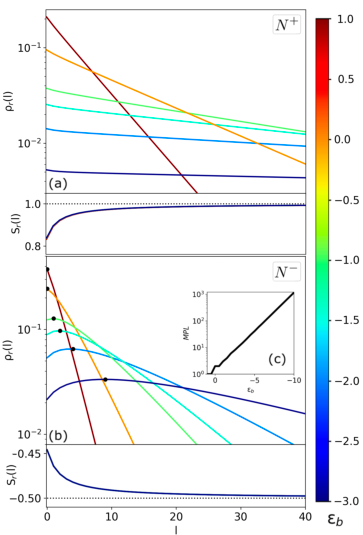
\includegraphics[width=0.5 \linewidth]{figures/chapter-2/FIG2}
  \caption[Polymer molecular-weight distributions $\rho_{r \ell}$ and corresponding  uniaxial nematic order parameter $S_{r \ell}$ as a function of the polymer length $\ell$ ]{Polymer molecular-weight distributions $\rho_{r \ell}$ and corresponding  uniaxial nematic order parameter $S_{r \ell}$ as a function of the polymer length $\ell$ for (a) a typical polymer nematic $N^{+}$ and (b) discotic nematic phase $N^{-}$. The effective temperature $\varepsilon_{b}$ is color-coded.
  (c) Most Probable Length (MPL) in terms of the effective temperature $\varepsilon_{b}$. Fixed parameters: persistence length $\ell_{p} = 3$, disc mole fraction $x = 0.5$, overall concentration $\rho = 3$, excluded-volume {\em ratios} $q = \frac{1}{4}\frac{L_{r}}{D_{r}}$ and $z=\pi q$ with monomer aspect ratio $L_{r}/D_{r} =10$.  }
  \label{fig:distributions}
\end{SCfigure}
 
Let us now examine a concrete example by picking a dense uniaxial discotic nematic  doped with polymerizing rods. The polymers are dispersed anti-nematically within the discotic fluid as indicated in \fig{fig:cartoon}(e).   In specifying the shape of the rods and discs, we can distinguish between  so-called {\em symmetric} mixtures \cite{stroobants1984}, in which the excluded-volume  between two monomers, a monomer and a disc and two discs are all equal, so that $q = 1$ and $z = 1$ and {\em asymmetric mixtures} composed of species with  strongly disparate excluded volumes.   Our principal attention goes to the latter systems which arise more naturally in an experimental context when mixing, for instance, tip-associating colloidal rods such as {\em fd} \cite{fraden-tmv-baus,dogic-fraden_fil} with clay platelets \cite{davidson-overview}. The molecular-weight distributions of some mixtures of this nature are shown in \fig{fig:distributions}.

 \fig{fig:distributions}(a) relates to the uniaxial polymer-dominated nematic phase ($N^+$) and demonstrates an exponential probability distribution  whose shape can be tuned by changing the effective temperature of the system. As expected, the tail of the distribution grows upon decreasing the temperature, which would give longer polymers. A more interesting scenario shows up for the discotic nematic phase ($N^-$) in \fig{fig:distributions}(b), where the distributions are no longer monotonically decreasing. The maximum of the distributions corresponds to the most probable length of the polymers for each system, which depends quite sensitively on the effective temperature as we  observe in \fig{fig:distributions}(c). Reversible polymerization within an anti-nematically organization  thus leads to a strong manifestation of oligomeric polymers at the expense of its monomeric counterparts. We  note that the orientational order associated with the anti-nematic oligomers remains relatively mild (particularly at larger temperature $\varepsilon_{b}$) so that the second-polynomial truncation should not be too severe.


As we will see during the incoming sections of this chapter, the overall particle concentration and disc molar fraction  associated with \fig{fig:distributions} may correspond to  regions of the phase diagram where the uniform nematic system is in fact thermodynamically unstable with respect to some kind of phase separation. The molecular-weight distributions should therefore be interpreted under the caveat that monophasic nematic fluidity is preserved and that any demixing process is somehow suppressed. We wish to add that the non-monotonic features of the anti-nematic polymer molecular-weight distribution are also present at conditions where monophasic anti-nematic order is found to be stable.  Next we address the  thermodynamic stability of the mixtures  within the context of a Gaussian variational theory. 

\section{Isotropic-nematic phase behavior}

At conditions where (anti-)nematic order is strong, the previously used polynomial-based expansion truncated after ${\mathcal P}_{2}$ [\eq{p2expansion}] is no longer appropriate and  a cumbersome inclusion of multiple higher-order terms becomes necessary \cite{lekkerkerker84,wensinkbiaxial}. A more technically expedient route towards exploring the thermodynamics of strongly ordered nematic fluids is to use a simple Gaussian parameterization of the orientational probability \cite{odijkoverview,Vroege92}.  Following \cite{wensink_mm2019} we express the polymer molecular-weight distribution in a factorized form:
\beq
\rho_{r} (\ell , \oma ) = \rho_{r \ell} f_{G} (\oma) 
\label{pfac}
\eeq
where $f_{G}$ is a normalized Gaussian distribution with a variational parameter that is proportional to either the degree of nematic  order ($\alpha^{(1)} > 0$) or anti-nematic order  ($\alpha^{(2)} > 0$).  The corresponding Gaussian distributions for the polar angles corresponding to these different nematic symmetries are given by \cite{wensinkrodplate}:
\beq
f_{G} (\oma) \sim  
\begin{cases}
\frac{\alpha^{(1)}}{4 \pi } \exp (-\frac{1}{2}\alpha^{(1)} \theta^{2} ) , \\
\sqrt{ \frac{ \alpha^{(2)} }{ (2 \pi )^{3} } } \exp (-\frac{1}{2} \alpha^{(2)} \psi^{2} )
\end{cases}
\label{gaussians}
\eeq
where $\psi = \frac{\pi}{2} - \theta$ ($-\pi/2 < \psi < \pi/2$) denotes a polar angle (see \fig{fig:cartoon}a). The Gaussians operate on the domain $0 < \theta < \pi/2$ and must be complemented by their mirror $f_{G} (\pi - \theta )$ for $\pi/2 < \theta < \pi$  given that all nematic phases are required to be strictly apolar. The Gaussian representations are appropriate only for strong nematic order ($\alpha \gg 1$). They are clearly inadequate for isotropic systems since the probabilities reduce to zero when $\alpha \rightarrow 0$ instead of reaching a constant.  Obviously,  we  apply the same distributions to the discs with $\alpha_{d}^{(1)}$ and $\alpha_{d}^{(2)}$ denoting the variational parameters quantifying the amount of (anti)nematic order of the discs. The disc probability density is then equivalent to \eq{pfac}:
\beq
\rho_{d} (\oma ) = \rho_{d0} f_{G} (\oma) 
\eeq
A major advantage of using  Gaussian trial functions is that we may apply  asymptotic expansion of the various free energy contributions \cite{odijkoverview} which are valid in the limit $\alpha \rightarrow \infty$. In particular, it can be shown that the double orientational averages over the sine and cosine in \eq{fex} up to leading order in $\alpha$ take a simple analytic form \cite{wensinkrodplate}.  In the general case in which particles with equal nematic signature (nematic or anti-nematic) do not necessarily have the same degree of alignment the asymptotic averages read:
\begin{align}
\langle \langle | \sin \gamma | \rangle \rangle_{11} & \sim \sqrt{ \frac{\pi}{2} \left ( \frac{1}{\alpha^{(1)}} + \frac{1}{\alpha^{(1\prime)}} \right ) } \nonumber \\  
    \langle \langle | \cos \gamma | \rangle \rangle_{12} & \sim  \sqrt{ \frac{2}{\pi} \left ( \frac{1}{\alpha^{(1)}} + \frac{1}{\alpha^{(2)}} \right ) } \nonumber \\ 
    \langle \langle | \sin \gamma | \rangle \rangle_{22} & \sim \mathcal{F} (\alpha^{(2)}, \alpha^{(2\prime)})
    \label{sinav}
\end{align}
Here,  the double brackets denote the orientational averages featuring in the excess free energy \eq{fex} with $ \langle \cdot \rangle = \int d \oma f_{G} (\oma) $. The symmetry of nematic order clearly matters since the anti-nematic case features a distinct logarithmic dependence. The function ${\mathcal F}$ reads in explicit form:

\beq
 {\mathcal F}(\alpha^{(2)},\alpha^{(2 \prime)} ) = \frac{4 \alpha^{(2)} Q -2 (1+Q) \textrm{arctanh} \sqrt{Q}  - (1+Q) \ln (1-Q) +(1+Q) \ln ( 4 \alpha^{(2)} Q) } {2 \pi \alpha^{(2)} Q}
\eeq

in terms of the ratio $Q=  \alpha^{(2\prime)}/ \alpha^{(2)}$ with $\alpha^{(2)}$ and $\alpha^{(2\prime)}$ quantifying the anti-nematic order parameters of two polymeric species differing in length. Note that generally, $\alpha^{(2)} \neq \alpha^{(2\prime)}$. The expression becomes a lot more manageable if all polymers are assumed to exhibit an equal degree of alignment, irrespective of their length. Then, $Q=1$ and \cite{wensink2001}:
\beq
{\mathcal F}(\alpha^{(2)})  =  \frac{2}{\pi} \left ( 1 + \frac{\ln \alpha^{(2)}}{2 \alpha^{(2)}} \right )
\eeq
Similar asymptotic expressions may be obtained for the orientational entropy featuring in the ideal free energy \eq{free}. For strong nematic or anti-nematic order we find, respectively \cite{wensinkrodplate}:
\begin{align}
\sigma_{1} = \langle \ln 4 \pi f_{G} (\oma) \rangle_{1} &\sim \ln \alpha^{(1)} -1  \nonumber \\
\sigma_{2} =\langle \ln 4 \pi f_{G} (\oma) \rangle_{2}   &\sim \frac{1}{2} \left ( \ln \alpha^{(2)} + \ln \frac{2}{\pi} -1 \right )  
\label{sigma12}
\end{align}
The worm-like chain entropy \eq{wlc} too can be quantified within the Gaussian limit which leads to:
\begin{align}
\langle  f_{G}^{1/2} (\oma) \nabla^{2} f_{G}^{1/2} (\oma)  \rangle_{1} & \sim -\frac{\alpha^{(1)}}{2} \nonumber \\ 
\langle  f_{G}^{1/2} (\oma) \nabla^{2}  f_{G}^{1/2} (\oma)  \rangle_{2} & \sim  
-\frac{\alpha^{(2)}}{4} 
\end{align}
We infer that the loss of conformational entropy of an {\em anti-nematic} polymer is half that of a nematic polymer. This suggests that a worm-like chain is able to retain more of its internal configurations when aligned anti-nematically than in a nematic organization of equal strength. With all the orientational averages specified, we  now turn to computing the free energy and its derivatives. 



\subsection{Polymer nematic phase ($N^{+}$)}

We first focus on the case of the polymer-dominated nematic phase which is expected to be stable at elevated monomer concentration and low disc mole fraction.  Inserting the asymptotic orientational averages formulated above into the corresponding entropic contributions in \eq{free} we obtain the following algebraic expression for the free energy density (in units thermal energy $k_{B}T$ per randomized monomer excluded volume $v_{rr}$):
\begin{align}
   & \frac{F^{N^{+}}}{V}  \sim  \sum_{\ell }  \rho_{r \ell} \ell^{-1}  \left [ \ln \rho_{r \ell} \ell^{-1}  -1 - \varepsilon_{b}  + \sigma_{1}(\alpha_{r \ell}) \right ] \nonumber \\
   & + \rho_{d0} \left [ \ln \rho_{d0} -1 + \sigma_{2}(\alpha_{d}) \right ]  \nonumber \\ 
    & + \frac{1}{3\ell_{p}} \sum_{\ell } \rho_{r \ell} \alpha_{r \ell} + \sum_{\ell,\ell^{\prime}} \rho_{r \ell} \rho_{r \ell^{\prime}} h_{r\ell r\ellp} \nonumber \\
    & + 2 q \rho_{d0} \sum_{\ell} \rho_{r \ell} h_{r\ell d} + z \rho_{d0}^{2} \frac{8}{\pi^{2}} \left ( 1+ \frac{\ln \alpha_{d}}{2 \alpha_{d}}   \right ) 
\end{align}
with $h_{ij}$ is short-hand notation for:
\beq
h_{ij} = \sqrt{ \frac{8}{\pi}   \left ( \frac{1}{\alpha_{i}} + \frac{1}{\alpha_{j}} \right )} 
\eeq
where $\alpha_{i}$ and $\alpha_{j}$ should be considered dummy variables for the species-dependent nematic order parameters as specified by the indices $i$ and $j$. 
For later reference we also define:
\beq
g_{ij} = \left (  \frac{8}{\pi} \right)^{1/2}  \left ( 1+ \frac{\alpha_{i} }{\alpha_{j }} \right )^{-1/2}
\eeq
At equilibrium, the species-dependent nematic order parameters $\alpha_{r\ell}$ and $\alpha_{d}$ follow from the minimum conditions:
\begin{align}
    \frac{\partial F/V}{\partial \alpha_{r \ell,d}} &=0 
    \label{dalpha}
\end{align}
The expressions above can be simplified considerably by noting that a small amount  of backbone flexibility causes the nematic alignment to fully decorrelate from the polymer contour length. We then approximate $\alpha_{r \ell} \approx \alpha_{r \ell^{\prime}} = \alpha_{r}$, independent from $\ell$.   Applying \eq{dalpha} we obtain a set of simple algebraic equations:
\begin{align}
      m_{N^{+}}^{-1} \alpha_{r}^{1/2}  &= - \frac{1}{3\ell_{p}} \alpha_{r}^{3/2} + \frac{2}{\sqrt{\pi}}  \rho_{r0} + q \rho_{d0}  g_{rd} \nonumber \\
         \alpha_{d}^{1/2} &=  z \rho_{d0} \frac{8}{\pi^{2}}\left (  \frac{ \ln \alpha_{d} -1}{\alpha_{d}^{1/2}} \right ) 
  + 4 q \rho_{r0} g_{dr} 
  \label{alphaplus}
\end{align}
with $m_{N^{+}}$ the mean aggregation number in the polymer nematic phase.
The  molecular-weight distribution  now becomes strictly exponential, as for the isotropic phase. We write:
\begin{align}
\rho_{r \ell } & = \ell e^{ \tilde{\varepsilon}_{b}} \left ( 1 - m_{N^{+}}^{-1} \right ) ^{\ell} \label{disn}
\end{align}
with an {\em effective} potential $\tilde{\varepsilon}_{b}$ that depends on the orientational entropy:
\beq
\tilde{\varepsilon}_{b} = \varepsilon_{b} - \sigma_{1}(\alpha_{r}) 
\label{tempnplus}
\eeq
Given that $\sigma_{1} >0$, the effective temperature is {\em lower} than the bare one, so that polymerization in the nematic phase is stronger than in the isotropic fluid, as is well established \cite{vdschoot1994epl,vdschoot1994la}. The mean aggregation number in the nematic phase  has an analogous form to \eq{miso}):
\beq
m_{N^{+}}  = \frac{1}{2} \left ( 1+ \sqrt{1+ 4 \rho_{r0} e^{-\tilde{\varepsilon}_{b}} }\right ) 
\eeq
The chemical potentials are obtained from the standard thermodynamic relations $\mu_{r,d}  = \partial (F/V) /\partial \rho_{r0,d0}$. The contribution from the polymers reads:
\begin{align}
\mu_{r}^{N^{+}}  \sim & \ln ( 1 - m_{N^{+}}^{-1}) + \frac{1}{3 \ell_{p}}  +  m_{N^{+}}^{-1} \sigma_{1}(\alpha_{r})  \nonumber \\
& + 2  \rho_{r0}   \frac{4}{\sqrt{\pi \alpha_{r}}}  +   2 q \rho_{d0} h_{rd}
+ \varepsilon_{b} 
\end{align}
while for the discs we find:
\begin{align}
\mu_{d}^{N^{+}}  \sim  & \ln \rho_{d0}  + \sigma_{2}(\alpha_{d})  +   2 q \rho_{r0}  
h_{rd} + 2 z \rho_{d0} 
\frac{8}{\pi^{2}} \left ( 1+ \frac{\ln \alpha_{d}}{2 \alpha_{d}} \right )
\end{align}
The osmotic pressure follows from  the thermodynamic relation $-P = (F - N \mu)/V$ leading to:
\begin{align}
P^{N^{+}} \sim & e^{\tilde{\varepsilon}_{b}} (m_{N^{+}} -1) 
+ \rho_{d0}  +  \rho_{r0}^{2}  \frac{4}{\sqrt{\pi \alpha_{r}}}
 \nonumber \\ 
& +   2 q \rho_{r0}  \rho_{d0} h_{rd}
 + z \rho_{d0}^{2} 
  \frac{8}{\pi^{2}} \left ( 1+ \frac{\ln \alpha_{d}}{2 \alpha_{d}}   \right )
\label{pressurenp}
\end{align}
Note that all pressures are implicitly renormalized in units of the thermal energy $k_{B}T$ per monomer excluded volume  $v_{rr}$.


\subsection{Discotic nematic phase ($N^{-}$)}

Repeating the previous steps for the discotic nematic through simple bookkeeping we write for the free energy of the discotic phase:
\begin{align}
   & \frac{F^{N^{-}}}{V}  \sim  \sum_{\ell }  \rho_{r \ell} \ell^{-1}  \left [ \ln \rho_{r \ell} \ell^{-1}  -1 - \varepsilon_{b}  +\sigma_{2} (\alpha_{r \ell})  \right ] \nonumber \\
   & + \rho_{d0} [ \ln \rho_{d0} -1 + \sigma_{1}(\alpha_{d})  ] + \frac{1}{6\ell_{p}} \sum_{\ell } \rho_{r \ell} \alpha_{r \ell} \nonumber \\ 
   & + \sum_{\ell,\ell^{\prime}} \rho_{r \ell} \rho_{r \ell^{\prime}} 
    \frac{4}{\pi} {\mathcal F} (\alpha_{r \ell}, \alpha_{r \ell^{\prime}}) \nonumber \\
    & + 2 q \rho_{d0} \sum_{\ell} \rho_{r \ell}  h_{r\ell d} + z \rho_{d0}^{2} \frac{4} {\sqrt{ \pi \alpha_{d}}}
\end{align}
The corresponding minimum conditions for the variational parameters under the assumption that all polymer species experience the same degree of orientational order ($\alpha_{r \ell} = \alpha_{r \ell \prime} = \alpha_{r}$) are as follows: 
\begin{align}
     \frac{1}{2} m_{N^{-}}^{-1}  \alpha_{r }^{1/2} &=  - \frac{1}{6\ell_{p}} \alpha_{r }^{3/2} +  \rho_{r0}  \frac{8}{\pi^{2}} 
    \left ( \frac{\ln  \alpha_{r} - 1}{\alpha_{r}^{1/2}} \right )   + q \rho_{d0}  g_{rd} \nonumber \\
 \alpha_{d}^{1/2} &=  z \rho_{d0} \frac{2}{\pi^{1/2}}  + 2 q \rho_{r0} g_{dr}
 \label{alphamin}
\end{align}
The molecular-weight distribution is  analogous to \eq{disn} but with the effective temperature now reading:
\beq
\tilde{\varepsilon}_{b} = \varepsilon_{b} - \sigma_{2}(\alpha_{r}) 
\label{tempnmin}
\eeq
which, as for the case of the polymer nematic phase suggests that particle alignment facilitates polymer growth, although less so for anti-nematic polymers since generally $\sigma_{2}  < \sigma_{1}$ (\eq{sigma12}).  The chemical potential of the polymers and the discs are given by, respectively:
\begin{align}
 \mu_{r}^{N^{-}}   \sim  
& \ln ( 1 - m_{N^{-}}^{-1}) + \frac{1}{6 \ell_{p}}  +  m_{N^{-}}^{-1} \sigma_{2}(\alpha_{r})  \nonumber \\
& + 2  \rho_{r0} 
\frac{8}{\pi^{2}} \left ( 1+ \frac{\ln \alpha_{r}}{2 \alpha_{r}} \right )
+   2 q \rho_{d0}  h_{rd}
+ \varepsilon_{b} \nonumber \\
 \mu_{d}^{N^{-}}  \sim  & \ln \rho_{d0}  + \sigma_{1}(\alpha_{d})  +   2 q \rho_{r0}  
h_{rd} + 2 z \rho_{d0}  \frac{4} {\sqrt{ \pi \alpha_{d}}}
\end{align}
Finally, the pressure of the $N^{-}$ phase reads:
\begin{align}
P^{N^{-}} \sim & e^{\tilde{\varepsilon}_{b}} (m_{N^{-}} -1) + \rho_{d0} +  \rho_{r0}^{2}  \frac{8}{\pi^{2}} \left ( 1+ \frac{\ln \alpha_{r}}{2 \alpha_{r}}   \right )
 \nonumber \\ 
& +   2 q \rho_{r0}  \rho_{d0}  h_{rd}
 + z \rho_{d0}^{2}  \frac{4}{\sqrt{\pi \alpha_{d}}}
\label{pressurenm} 
\end{align}
The thermodynamics of the isotropic phase is easily established from the original free energy \eq{free} because the randomized excluded volumes becomes simple constants, namely  $\langle \langle | \sin \gamma | \rangle \rangle = \pi/4$ and $\langle \langle  | \cos \gamma | \rangle \rangle  = 1/2$. We thus obtain the following expressions for the chemical potentials in the isotropic fluid \cite{wensink_mm2019}:
\begin{align}
  \mu_{r}^{\textrm I} & \sim  \ln ( 1- m_{I}^{-1} )  + 2  \rho_{r0}  +   2 q \rho_{d0}  + \varepsilon_{b} \nonumber \\
   \mu_{d}^{\textrm I} & \sim \ln \rho_{d0}  +   2 z \rho_{d0} + 2 q \rho_{r0} 
  \end{align}
The osmotic pressure  combines the ideal gas and excluded volume contributions and reads:
\begin{align}
   P^{\textrm I}  &\sim  e^{\varepsilon_{b}} (m_{I} -1) + \rho_{d0}  +  \rho_{r0}^{2}
+   2 q \rho_{r0}  \rho_{d0}  + z \rho_{d0}^{2} 
\end{align}
Binodals denoting coexistence between phases of any symmetry may be established from equating chemical potentials and pressures in conjunction with the minimum conditions for the nematic variational parameters, where relevant.  Phase diagrams can be represented in a pressure-composition  ($P-x$) plane or, alternatively, in a density-density representation using $\rho_{r0} = c (1-x)$ and $\rho_{d0}  = cx$ in terms of the overall particle concentration $c$ and disc mole fraction ($0<x<1$). In order to remain consistent with the Gaussian approximation adopted in our analysis, we will focus on {\em asymmetric} mixtures characterized by both monomer-disc and disc-disc excluded volumes being much larger than the monomer-monomer one. The considerable excluded-volume disparity thus ensures that the nematic order of all components be sufficiently strong. Concretely, we impose that $\alpha_{r,d} >5$  for all numerical results to be self-consistent. 


\section{Phase diagrams}

\begin{figure*}[ht]
  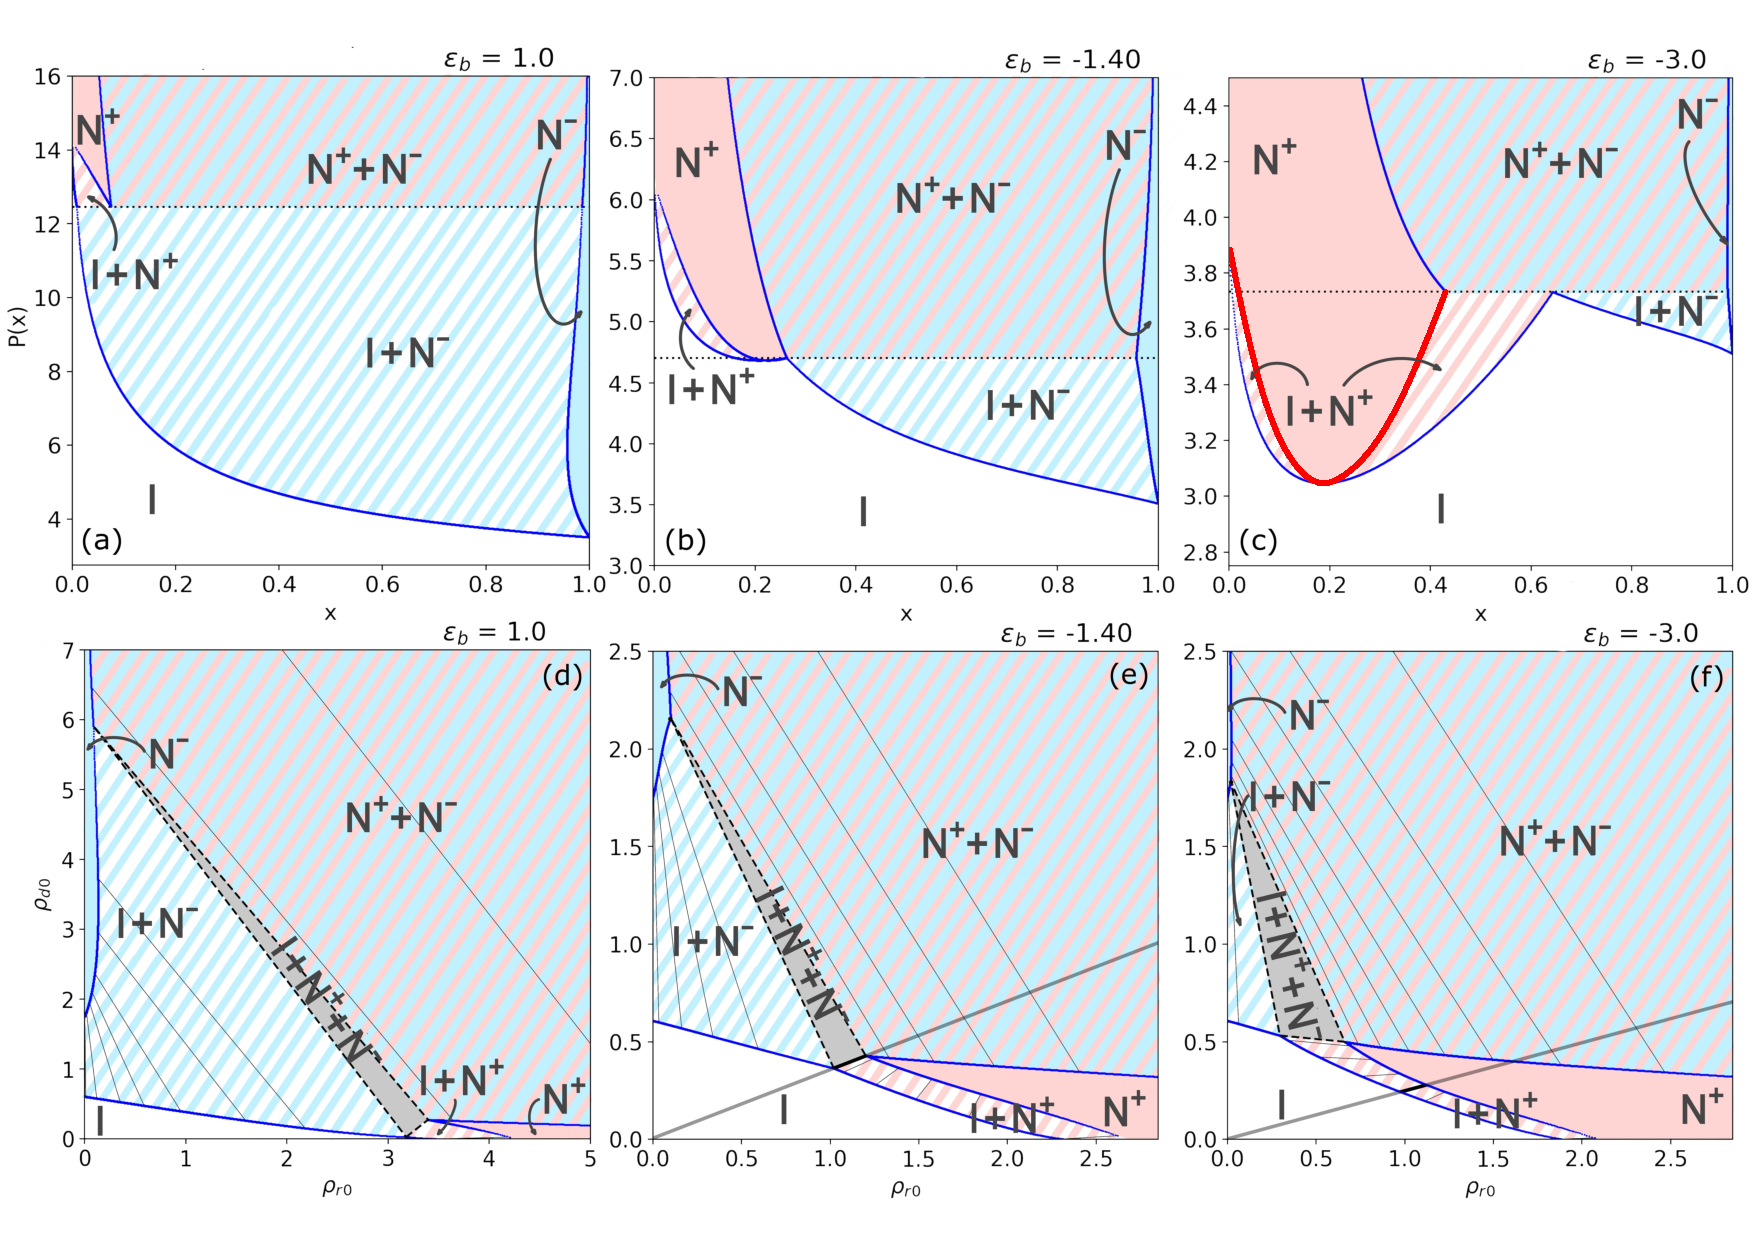
\includegraphics[width=\textwidth]{figures/chapter-2/FIG3}
  \caption[Overview of the isotropic $I$ (white) -  polymer nematic $N^+$ (red) - discotic nematic $N^-$ (blue) phase diagrams for a mixture of]{Overview of the isotropic $I$ (white) -  polymer nematic $N^+$ (red) - discotic nematic $N^-$ (blue) phase diagrams for a mixture of discs and reversibly polymerizing weakly flexible rods at various effective temperatures $\varepsilon_{b}$. Two types of phase diagrams are represented: osmotic pressure $P$ versus disc mole fraction $x$ (top panels) and concentration of discs $\rho_{d0}$ versus concentration of rods $\rho_{r0}$ (bottom panels). Fixed parameters: persistence length $\ell_{p} = 3$, excluded-volume {\em ratios} $q = \frac{1}{4}\frac{L_{r}}{D_{r}}$ and $z=\pi q$ where $L_{r}/D_{r} =10$. The presence of a negative {\em azeotrope} is indicated in panels (e) and (f) as a bold black line, which is shown to be parallel to the dilution line (grey diagonal shown in (e) and (f)).}
  \label{fig:L10}
\end{figure*}


\fig{fig:L10} presents an overview of the isotropic-nematic phase diagram for a mixture of reversibly polymerizing rods and discs at three different temperatures.  The choice of excluded-volume parameter $q$ and $z$ is inspired by the typical dimensions of experimentally realizable anisotropic colloids, where the  monomeric rods and discs usually have {\em equal} largest dimensions ($L_{r} = D_{d}$). The monomer aspect ratio $L_{r}/D_{r}$ can be chosen freely but we fix it here at  $L_{r}/D_{r} = 10$. The disc aspect ratio is not constrained as long as the discs are sufficiently thin ($D_{d}/L_{d} \gg 1$). In this study we keep the persistence length fixed at $\ell_{p} =3$. We found that variations up to $\ell_{p} =10$ (corresponding to stiffer monomers) did not lead to major changes in the phase behavior.  For practical reasons we refrained from exploring the near-rigid rod limit ($\ell_{p} \rightarrow \infty$) which is known to cause the polymers to grow to unphysically large lengths \cite{vdschoot1994la}.

Several key trends in the phase diagrams can be discerned. First of all, \fig{fig:L10}(a) correspond to high-temperature scenario in which reversible polymerization happens on a very limited scale. The shape-dissimilar nature of the mixture translates into a phase diagram that is highly asymmetric about the equimolar point $x=0.5$. Second, demixing is  prominent given the large range of monomer-disc compositions where the mixture fractionates into strongly segregated uniaxial nematic phases [\fig{fig:L10}(a)]. Only at very low osmotic pressures, where particle exclusion effects are relatively weak, does the mixture remain miscible throughout the entire composition range. We further observe that the discotic nematic $N^{-}$ can be stabilized over a relatively broad pressure range, while the polymer nematic ($N^{+}$)  only features at elevated pressures, where polymerization is strong enough for the long polymers to align into a conventional nematic organization with the discs interspersed anti-nematically. The phase diagram also features a triple $I-N^{+}-N^{-}$ equilibrium in agreement with previous predictions  \cite{galindo2,wensinkrodplate} and experiment \cite{kooijlangmuir2000,woolston2015} for discs mixed with {\em non-}polymerizing rods. 

Reducing the temperature stimulates polymer growth and, consequently, enhances the stability window for the polymer-dominated nematic  [\fig{fig:L10}(b) and (c)]. Reversible polymerization thus renders the phase diagrams less asymmetric.  At the same time, the osmotic pressure (and concomitantly the particle concentrations) at which nematic order occurs drops significantly as polymerization becomes more prominent. Furthermore, the $I-N^{+}$ binodals develop a remarkable (negative) {\em azeotrope} which in \fig{fig:L10}(b) coincides with the triple pressure. Under these conditions,  coexistence occurs between a discotic nematic,  a polymer nematic and an isotropic fluid with the latter two having the same monomer-disc composition. At lower temperature the azeotrope comes out more prominently at $x\approx 0.2$ (\fig{fig:L10}(c)). In the density-density representations shown in the bottom panels, the azeotrope manifests itself at the point where the tie line connecting the monomer and discs concentrations of the coexisting $I$ and $N^{+}$ phases coincides with the dilution line. The latter are straight lines emanating from the origin along which the overall particle concentration changes but the monomer-disc composition is preserved.  It can  be gleaned that upon following a dilution line at, for instance, $x=0.2$  the sequence of phase transitions encountered depends strongly on temperature. At high temperature [\fig{fig:L10}(a)] the isotropic fluid first transforms into $N^{-}$, then develops a triphasic $I-N^{+}-N^{-}$ equilibrium. At low temperature, however, a polymer nematic is formed first, followed by a binematic $N^{+}-N^{-}$ coexistence while the triphasic equilibrium does not show up at all unless the monomer concentration is significantly increased.   \fig{fig:azeotrope} provides insight into the change of nematic order of the polymers and discs as well as the mean aggregation number of the $N^{+}$ across the azeotrope. In view of their considerable excluded volume, the discs are way more ordered than the polymers ($\alpha_{d} >\alpha_{r}$).  Increasing the  mole fraction of discs  reduces the nematic order of both components, though the decrease is much more significant for the discs than the change of $\alpha_{r}$ for the polymers which in fact develops a minimum at the azeotrope.

\begin{SCfigure}
  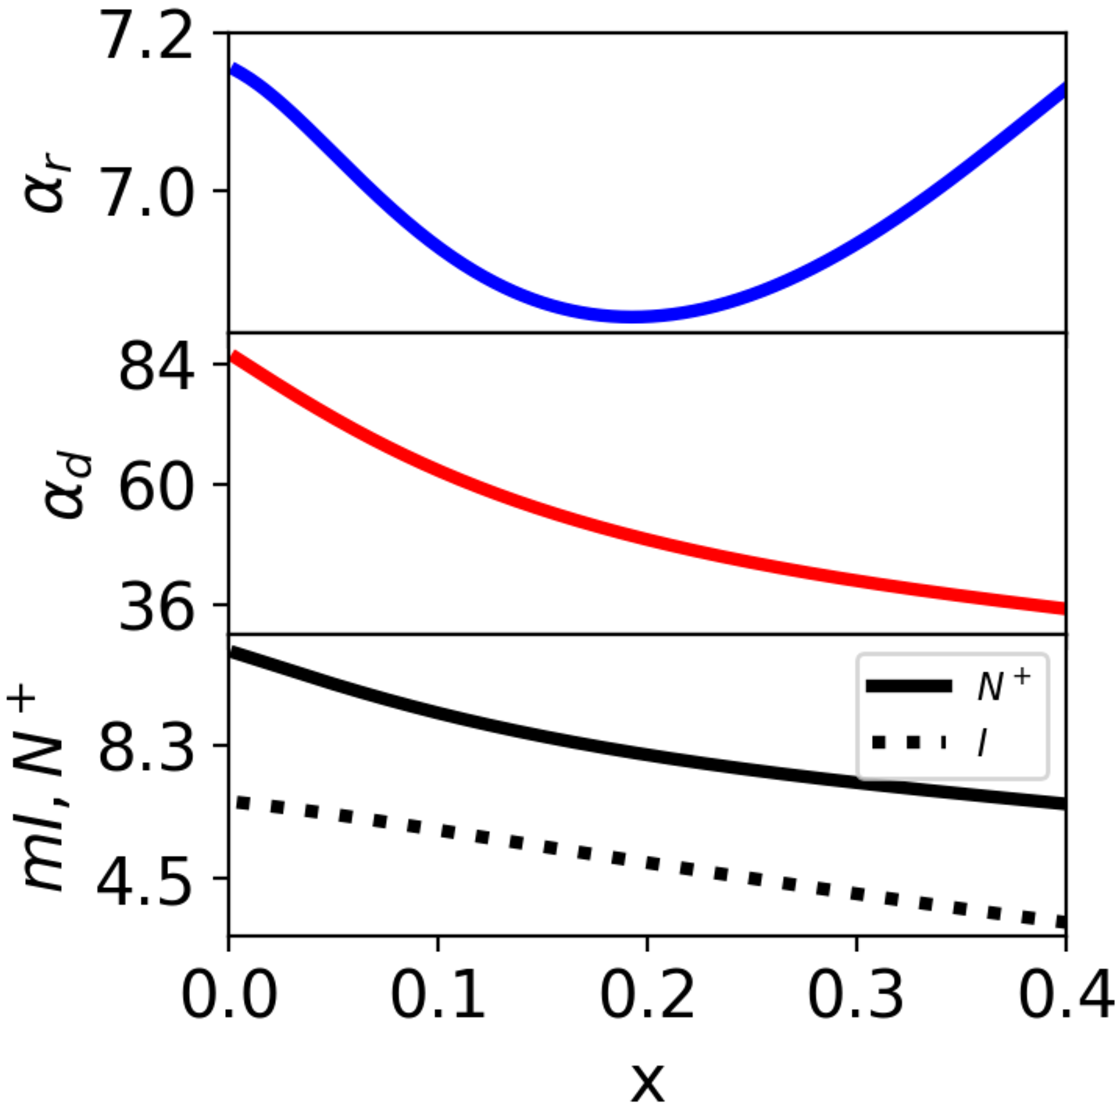
\includegraphics[width= .5\linewidth]{figures/chapter-2/FIG4}
\caption[Nematic order of the polymers ($\alpha_{r}$) and discs ($\alpha_{d}$) and polymer mean aggregation number ($m$) of  the nematic $N^{+}$ phase]{Nematic order of the polymers ($\alpha_{r}$) and discs ($\alpha_{d}$) and polymer mean aggregation number ($m$) of  the nematic $N^{+}$ phase in coexistence with the isotropic phase $I$  across the azeotropic region. The corresponding binodal in \fig{fig:L10}(c) has been indicated in red. }
  \label{fig:azeotrope}
\end{SCfigure}

\begin{figure*}[ht]
  \includegraphics[width= \linewidth]{figures/chapter-2/FIG5}
\caption[Phase diagram in the osmotic pressure-composition ($P-x$) representation with the following parameters:]{Phase diagram in the osmotic pressure-composition ($P-x$) representation with the following parameters: persistence length $\ell_{p} = 3$, effective temperature $\varepsilon_{b} = -1$, excluded-volume {\em ratios} $q = \frac{1}{4}\frac{L_{r}}{D_{r}}$ and $z=\pi q$ corresponding to a monomer aspect ratio $L_{r}/D_{r} =25$. The disc mole fraction $x$ is plotted on a linear scale (a) and on a logarithmic scale (b) to highlight the behavior close to single-component systems (pure polymers $x=0$, and pure discs $x=1$). Note the presence of a coexistence between an isotropic gas and fluid  phase ($I_1$ and $I_2$) with different discs compositions (grey region). (c) Comparison of mean aggregation numbers $m_{I}$ between $I_{1}$ and $I_{2}$ for a given pressure. $I_{1}$ corresponds to the phase at the lowest disc mole fraction $x$. }
  \label{fig:coexistence}
\end{figure*}

We move on to explore a similar mixture featuring more slender rod monomers, namely $L_{r}/D_{r} = 25$. The resulting phase diagram is shown in \fig{fig:coexistence}. The asymmetry of the mixture is now very strong with the monophasic  $N^{+}$ and $N^{-}$ regions being largely unstable except for strongly purified systems  ($x$ close to $0$ or $1$)  [\fig{fig:coexistence}(b)]. Qualitatively, the phase diagram resembles the one in \fig{fig:L10}(a), but the isotropic fluid  undergoes a gas-liquid-type phase separation producing two phases differing in composition. The $I_{1}$-phase may be associated with a discotic colloidal gas, and  $I_{2}$  with its liquid counterpart.   The demixing is driven by the extreme excluded-volume difference between the rod monomers and the discs. This phenomenon has been reported for (non-polymerizing) rod-disc mixtures in Ref. \cite{varga2002}, where the effect was ascribed to a {\em depletion} of discs by the much smaller rods. Isotropic-isotropic demixing has  been more generally observed when mixing different shapes dominated by hard-core repulsion \cite{dijkstra1994}, including thin and thick rods \cite{vanRoij97}, spheres and discs   \cite{chen2015,aliabadi2016} and discs  differing in diameter \cite{phillips_pre2010}. It has also been observed in thermotropic LC-solvent mixtures where the effect is primarily of enthalpic origin and is caused by specific interactions between the LC forming molecules and the solvent \cite{matsuyama1996,reyes2019}.  It is well known that mixing colloids with non-adsorbing polymer depletants creates an effective attraction between the colloids which is entirely of entropic origin and may drive various types of demixing mechanisms \cite{LekkerkerkerTuinier2011}. In our case, the depletion effect is however less clear-cut given that the ``depletants"   reversibly polymerize into a wide array of different sizes \cite{peters2021} and experience  orientation-dependent volume-exclusion interactions which are usually ignored in colloid-polymer models. Moreover the average polymer size depends, via \eq{miso}, on the monomer concentration which is different in the gas and liquid phases. \fig{fig:coexistence}(c) demonstrates that the difference in mean aggregation number between the two isotropic phases is in fact quite small, with the disc-rich fraction harboring slightly longer polymers.   Note that the presence of isotropic-isotropic demixing gives rise to a low-pressure triple equilibrium where both phases coexist with a discotic nematic $N^{-}$.  

\section{Quadruple fluid coexistence}

\begin{figure*}[ht]
  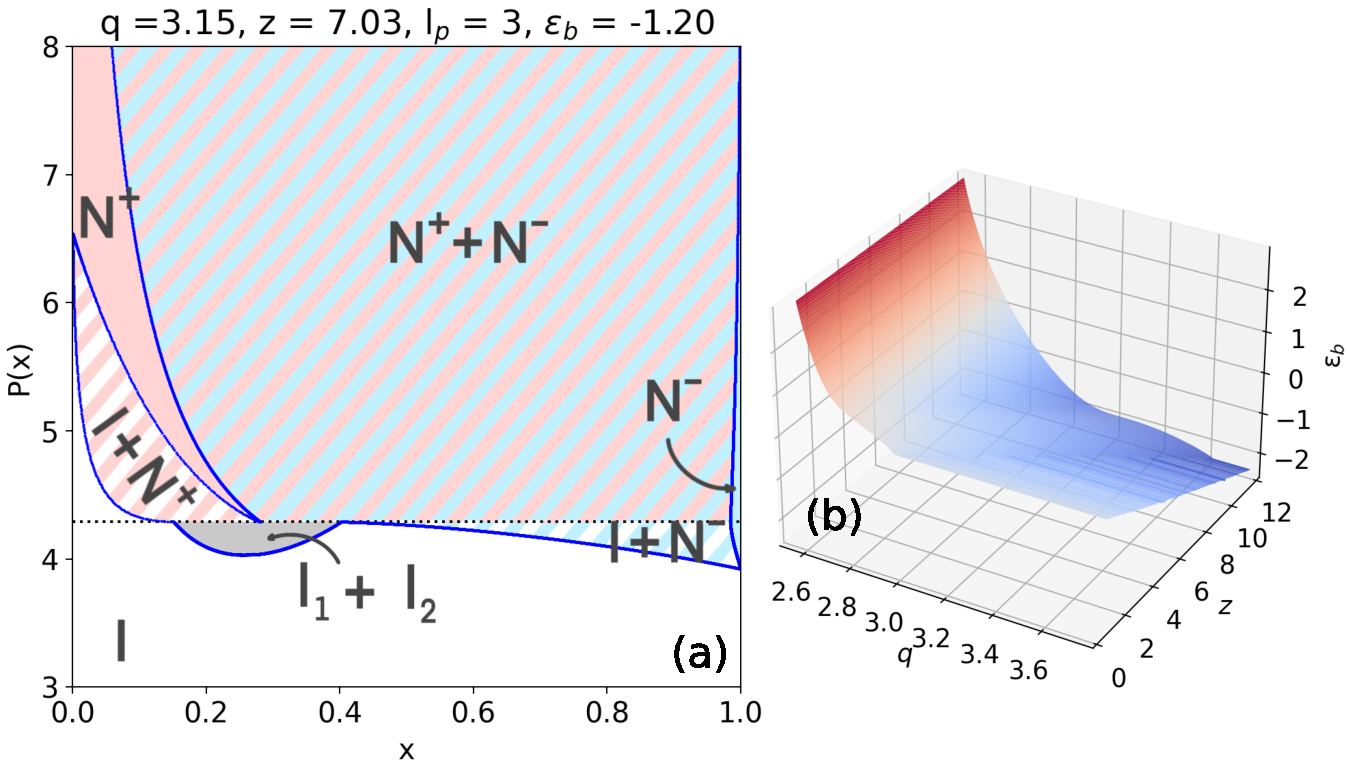
\includegraphics[width=0.9 \linewidth]{figures/chapter-2/FIG6}
\caption[Phase diagram in the osmotic pressure-composition showing a quadruple point]{(a) Phase diagram in the osmotic pressure-composition ($P-x$) representation showing an $I_{1}$-$I_{2}$-$N^{+}$-$N^{-}$ quadruple point at $P = 4.29$. For this particular case, $\ell_{p} = 3$, $\varepsilon_{b} = -1.2$, $L_{r}/D_{r} =25$ and $D_{d}/L_{r} = 0.7$. (b) Visualization of combinations of rod-disc excluded-volume ratio ($q$ and $z$) and temperature $\varepsilon_{b}$ where  an $I_{1}-I_{2}-N^{+}-N^{-}$ quadruple coexistence is possible.  }
\label{fig:qp}
\end{figure*}

At this stage, one might wonder whether a mixture could be designed in which  the two separate triple equilibria  in \fig{fig:coexistence} were to join into a  {\em quadruple} coexistence featuring all fluid phases. In \fig{fig:qp}(a) we demonstrate that this scenario is indeed possible. For the particular mixture shown there, the rod monomers and discs no longer have equal largest dimensions ($L_{r}= D_{d}$) but the disc diameter is somewhat smaller than the rod length, namely $D_{d} =0.7 L_{r}$ while the rods are kept sufficiently slender ($L_{r}/D_{r} = 25$). The  excluded-volume asymmetry is then sufficiently reduced to make the two triple points coincide and generate a simultaneous coexistence between two isotropic and two nematic phases, each differing in monomer-disc composition and overall particle concentration. This mixture is by no means  unique and belongs to a family of monomer-disc size ratios where a remarkable $I_{1}$-$I_{2}$-$N^{+}$-$N^{-}$ quadruple point could be encountered, as illustrated by the colored manifold in \fig{fig:qp}(b). This result provides important guidance if one wishes to explore these intricate multi-phase equilibria in real-life mixtures featuring reversibly polymerizing rods mixed with colloidal platelets.

 At this point we wish to draw a connection with recent theoretical explorations of polymer depletion on purely monomeric colloidal rods which have revealed similar multi-phase equilibria involving one-dimensional periodic smectic structures as well as fully crystalline states \cite{peters_prl2020}. Similar phenomena involving isotropic-nematic-columnar quadruple points had been reported previously for disc-polymer mixtures \cite{gonzalez2017}. In those studies, the multiphase equilibria emerge from an effective one-component theory based on free-volume theory where   polymeric depletants, envisaged as fixed-shape spherical particles that do not interact with one another, are depleted from the surface of the colloidal rod due to volume exclusion as per the original Asakura-Oosawa model \cite{ASAKURA54,ASAKURA58,Vrijdepletie}. In our work, the depletion effect is strongly convoluted since all components (polymer species and discs alike) are explicitly correlated, albeit on the simplified second-virial level. Furthermore, high-density crystal phases with long-ranged positional order are not considered in the present study since their stability requires strong uniformity in particle shape \cite{mederos_overview2014}, which is not the case in our mixtures. In fact, even for basic mixtures of non-associating hard rods mixed with hard discs the full phase behavior at conditions of elevated particle packing  remains largely elusive to this day. Large-scale  numerical simulations or density-functional computations are needed  to overcome the limitations of the simple second-virial approach taken here, but these are technically challenging to implement for dense multi-component systems. 
 
 The results gathered in \fig{fig:qp}  illustrates the possibility of generating four different fluid textures emerging from reversibly changing excluded-volume-driven interactions alone, without the need to invoke attractive interparticle forces. This could bear some relevance on the emergence of functionality through liquid-liquid type phase separation in biological cells which are composed of biomolecules possessing a multitude of different shapes, some of them  controlled by reversible association \cite{hyman2014,shin2017}.

\section{Conclusions}

We have explored the phase behaviour of a simple model for thermoresponsive supramolecular rods mixed with discotic particles. Possessing attractive tips the rod monomers reversibly associate into polymers that retain their basic slender rod shape and experience only a limited degree of backbone flexibility. The interaction between the species is assumed to be  of steric origin such that basic shape differences between the constituents, more specifically the excluded-volume disparity, plays a key role in determining the prevailing liquid crystal symmetry. The principal ones are a   polymer nematic ($N^{+}$) composed of nematic polymer interspersed with an anti-nematic organization of discs and a discotic nematic  ($N^{-}$) in which the polymers are dispersed anti-nematically.   Lowering   temperature stimulates  polymer growth which  enlarges the stability window for the $N^{+}$ phase.  The phase diagram  develops a marked {\em azeotrope} upon increasing the mole fraction of added discs which indicated that the  polymer nematic is stabilized by the addition of non-adsorbing rigid discs provided their mole fraction remains small. 
The polymer-dominated nematic phase eventually becomes destabilized at larger mole fractions where mutual disc alignment disrupts  the nematic  order of the polymers in favour of the formation of a discotic nematic phase in which the polymers self-organize into an anti-nematic structure. The corresponding molecular weight distribution functions strongly deviates from the usual exponential form and becomes non-monotonic with a maximum probability associated with oligomeric aggregates. Enhancing the shape-asymmetry between the rod monomers and discs we observe a depletion-driven demixing of the isotropic fluid which opens up the possibility of a quadruple existence featuring two isotropic phase along with the fractionated polymer and discotic nematic phases. Such quadruple points occur in a wide range of mixed-shape nematics involving supramolecular rods templated by discs and highlight the possibility of multiple liquid symmetries (both isotropic and anisotropic) coexisting in  mixtures of anisotropic colloids with reversible and thermoresponsive shape-asymmetry without cohesive interparticle forces.   Future explorations should aim at a more careful assessment of biaxial nematic order, ignored in the present study,  which could develop in near-equimolar rod-disc mixtures provided they are stable against global demixing (see Appendix \ref{appendix2A} for tentative discussion). Polymerizing rods and discs with finite particle thickness and low shape asymmetry may favor the emergence of liquid crystals possessing lamellar, columnar or fully crystalline signatures  \cite{peroukidis2010} which may be addressed using  computer simulation models along the lines of Refs. \cite{kuriabova2010,nguyen2014,perouklapp2020}. Inspiration for such mixed-shape  lamellar structures  could be drawn from bio-inspired supramolecular liquid crystals \cite{safinya2013} such as, for example, the `sliding columnar phase' and similar stacked architectures  observed in cationic liposome-DNA complexes \cite{wong2000,ohern1998} which are essentially made up of mixed planar and rod-shaped architectures.

\begin{subappendices}




\section{Renormalized ${\mathcal P}_{2}$ approximation for slightly flexible polymers}
\label{appendix2A}

We seek a simple perturbation theory for the one-body density   \eq{lnrhor}  of near-rigid polymers characterized by a finite persistence length $\ell_{p}$. Let us attempt the following generalization of the probability density distribution for the polymers: 
\beq
 \rho_{r} (\ell , \oma) =  \ell e^{\varepsilon_{b} + \lambda_{r} \ell} e^{ \ell (a_{r}+ \xi) \pp(\oma) }
\eeq
with $\xi$ representing a correction induced by the {\em internal} orientational entropy of the polymer due to a small degree of worm-like chain flexibility. 
Inserting this expression into the worm-like chain contribution (last term) in the EL equation  \eq{lnrhor},  substituting $\nabla^{2} = \partial_{t} (1-t^{2}) \partial_{t}$ and $t= \cos \theta$,  we find that for the uniaxial symmetry:
\begin{align}
\frac{\nabla^{2}  \rho_{r}^{1/2}}{  \rho_{r} ^{1/2} }  = & \frac{3}{4} \tilde{a}_{r}^{2} + \left  ( \frac{3}{2}  \tilde{a}_{r} ^{2}  - 3 \tilde{a}_{r} \right ) \pp(t) + {\mathcal O}(t^{4})
\label{roro1}
\end{align}
where $\tilde{a}_{r} = a_{r}  + \xi$ denotes a rescaled alignment amplitude for the polymer. 

\subsection*{Anti-nematic polymers}
We expect that neglecting the fourth-order term will be fairly harmless in a strongly anti-nematic state  where $t $ is generally very small (since $\theta \sim \pi/2 $ for most polymers). This situation is naturally encountered in the  $N^{-}$ phase where $a_{r} \ell \ll 0 $ in particular for the long polymers.  The constant  in \eq{roro1} is unimportant for the EL equation where it can be subsumed into the normalization factor $\lambda$, but must be retained when computing the worm-like chain free energy. Then, consistency requires that
\beq
\xi \approx  \frac{1}{3 \ell_{p}}  \left  ( \frac{3}{2}  \tilde{a}_{r} ^{2}  - 3 \tilde{a}_{r}  \right )
\eeq 
where the chain persistence length $\ell_{p}$ should be interpreted in units of the segment length $L_{r}$.  From the above the dependence of $\xi$ on the bare alignment amplitude $a_{r}$ is easily resolved and we find:
 \beq
 \xi \approx 1+ \ell_{p} +   |a_{r} |  -\sqrt{(1 +  \ell_{p})^{2} + 2 | a_{r} |  \ell_{p} }, \hspace{0.3cm} (a_{r} \ll 0 )
 \label{xi1}
 \eeq 
The correction factor vanishes in the rigid rod limit, $\lim_{\ell_{p} \rightarrow \infty} \xi = 0$, as it should.

\subsection*{Nematic polymers}

We may repeat the analysis for the case of conventional nematic polymers as encountered in the polymer-dominated $N^{+}$  phase using a slightly different route. For $a_{r} \gg 1$ the average polar deflection angle will be small and we may expand the worm-like chain term up to quadratic order in $\theta$. Using the asymptotic relation $\pp(t) \sim 1- 3\theta^{2}/2 $ and ignoring any constant factors we find a simple approximation valid for $|t|$ close to unity (strong alignment): 
\begin{align}
\frac{\nabla^{2}  \rho_{r}^{1/2}}{  \rho_{r} ^{1/2} }  \sim - \frac{3}{2} (  \tilde{a}_{r} ^{2}  + 2  \tilde{a}_{r} ) \pp(t) 
\label{roro2}
\end{align}
Then, in analogy with the preceding case we find an expression identical to \eq{xi1} except for a minus sign:
\beq
 -\xi \approx 1 + \ell_{p} + |a_{r}|  - \sqrt{(1 +  \ell_{p})^{2} + 2 |a_{r}|  \ell_{p}}, \hspace{0.3cm} (a_{r}  \gg 0)
\label{xi2}
\eeq
 This simple scaling result confirms our expectation, namely that a small degree of backbone flexibility leads to a reduction of the alignment propensity of the polymers, since $| a_{r} + \xi | $ is always smaller than $| a_{r}  |$. For strongly aligned systems, this effect turns out to be of equal strength for both nematic and anti-nematically ordered polymers.
 

\section{Stability of biaxial nematic order}
\label{appendix2B}

\begin{figure*}[ht]
  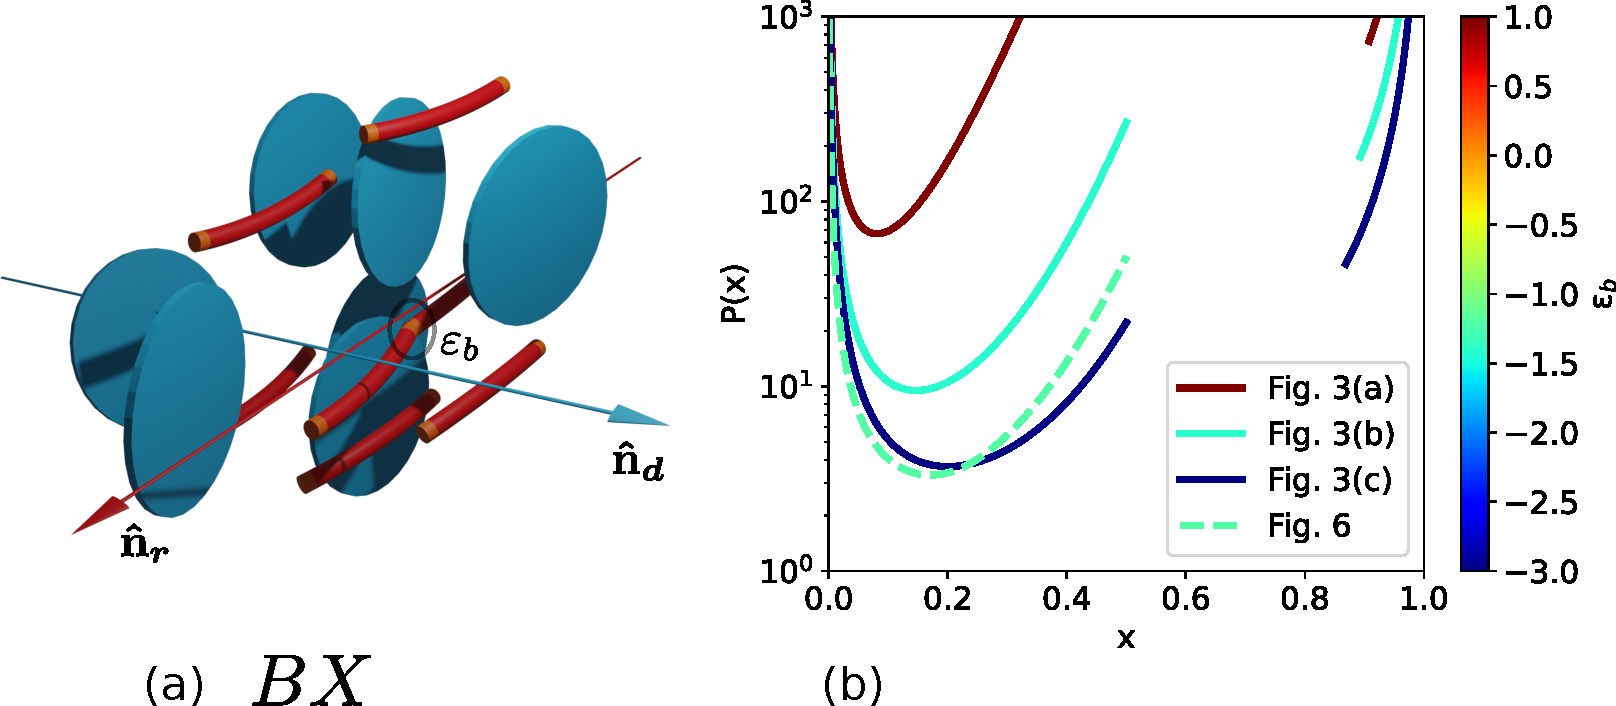
\includegraphics[width=.9 \textwidth]{figures/chapter-2/FIG7}
\caption[Schematic representation of the biaxial nematic phase $BX$ with orthorhombic ($D_{2h}$) point-group  symmetry]{(a) Schematic representation of the biaxial nematic phase $BX$ with orthorhombic ($D_{2h}$) point-group  symmetry, characterized by mutually perpendicular nematic directors for each species ($\bm{\hat{\textnormal{\bfseries n}}_r}$ for the polymers and $\bm{\hat{\textnormal{\bfseries n}}_d}$ for discs). (b) Bifurcation curves locating the transition from uniaxial (U) order at low osmotic pressure $P$ to biaxial (BX) nematic order at high pressure for a number of relevant cases studied in the main text. Here, $x$ denotes the disc mole fraction.  }
\label{fig:bx}
\end{figure*}



\begin{figure}
  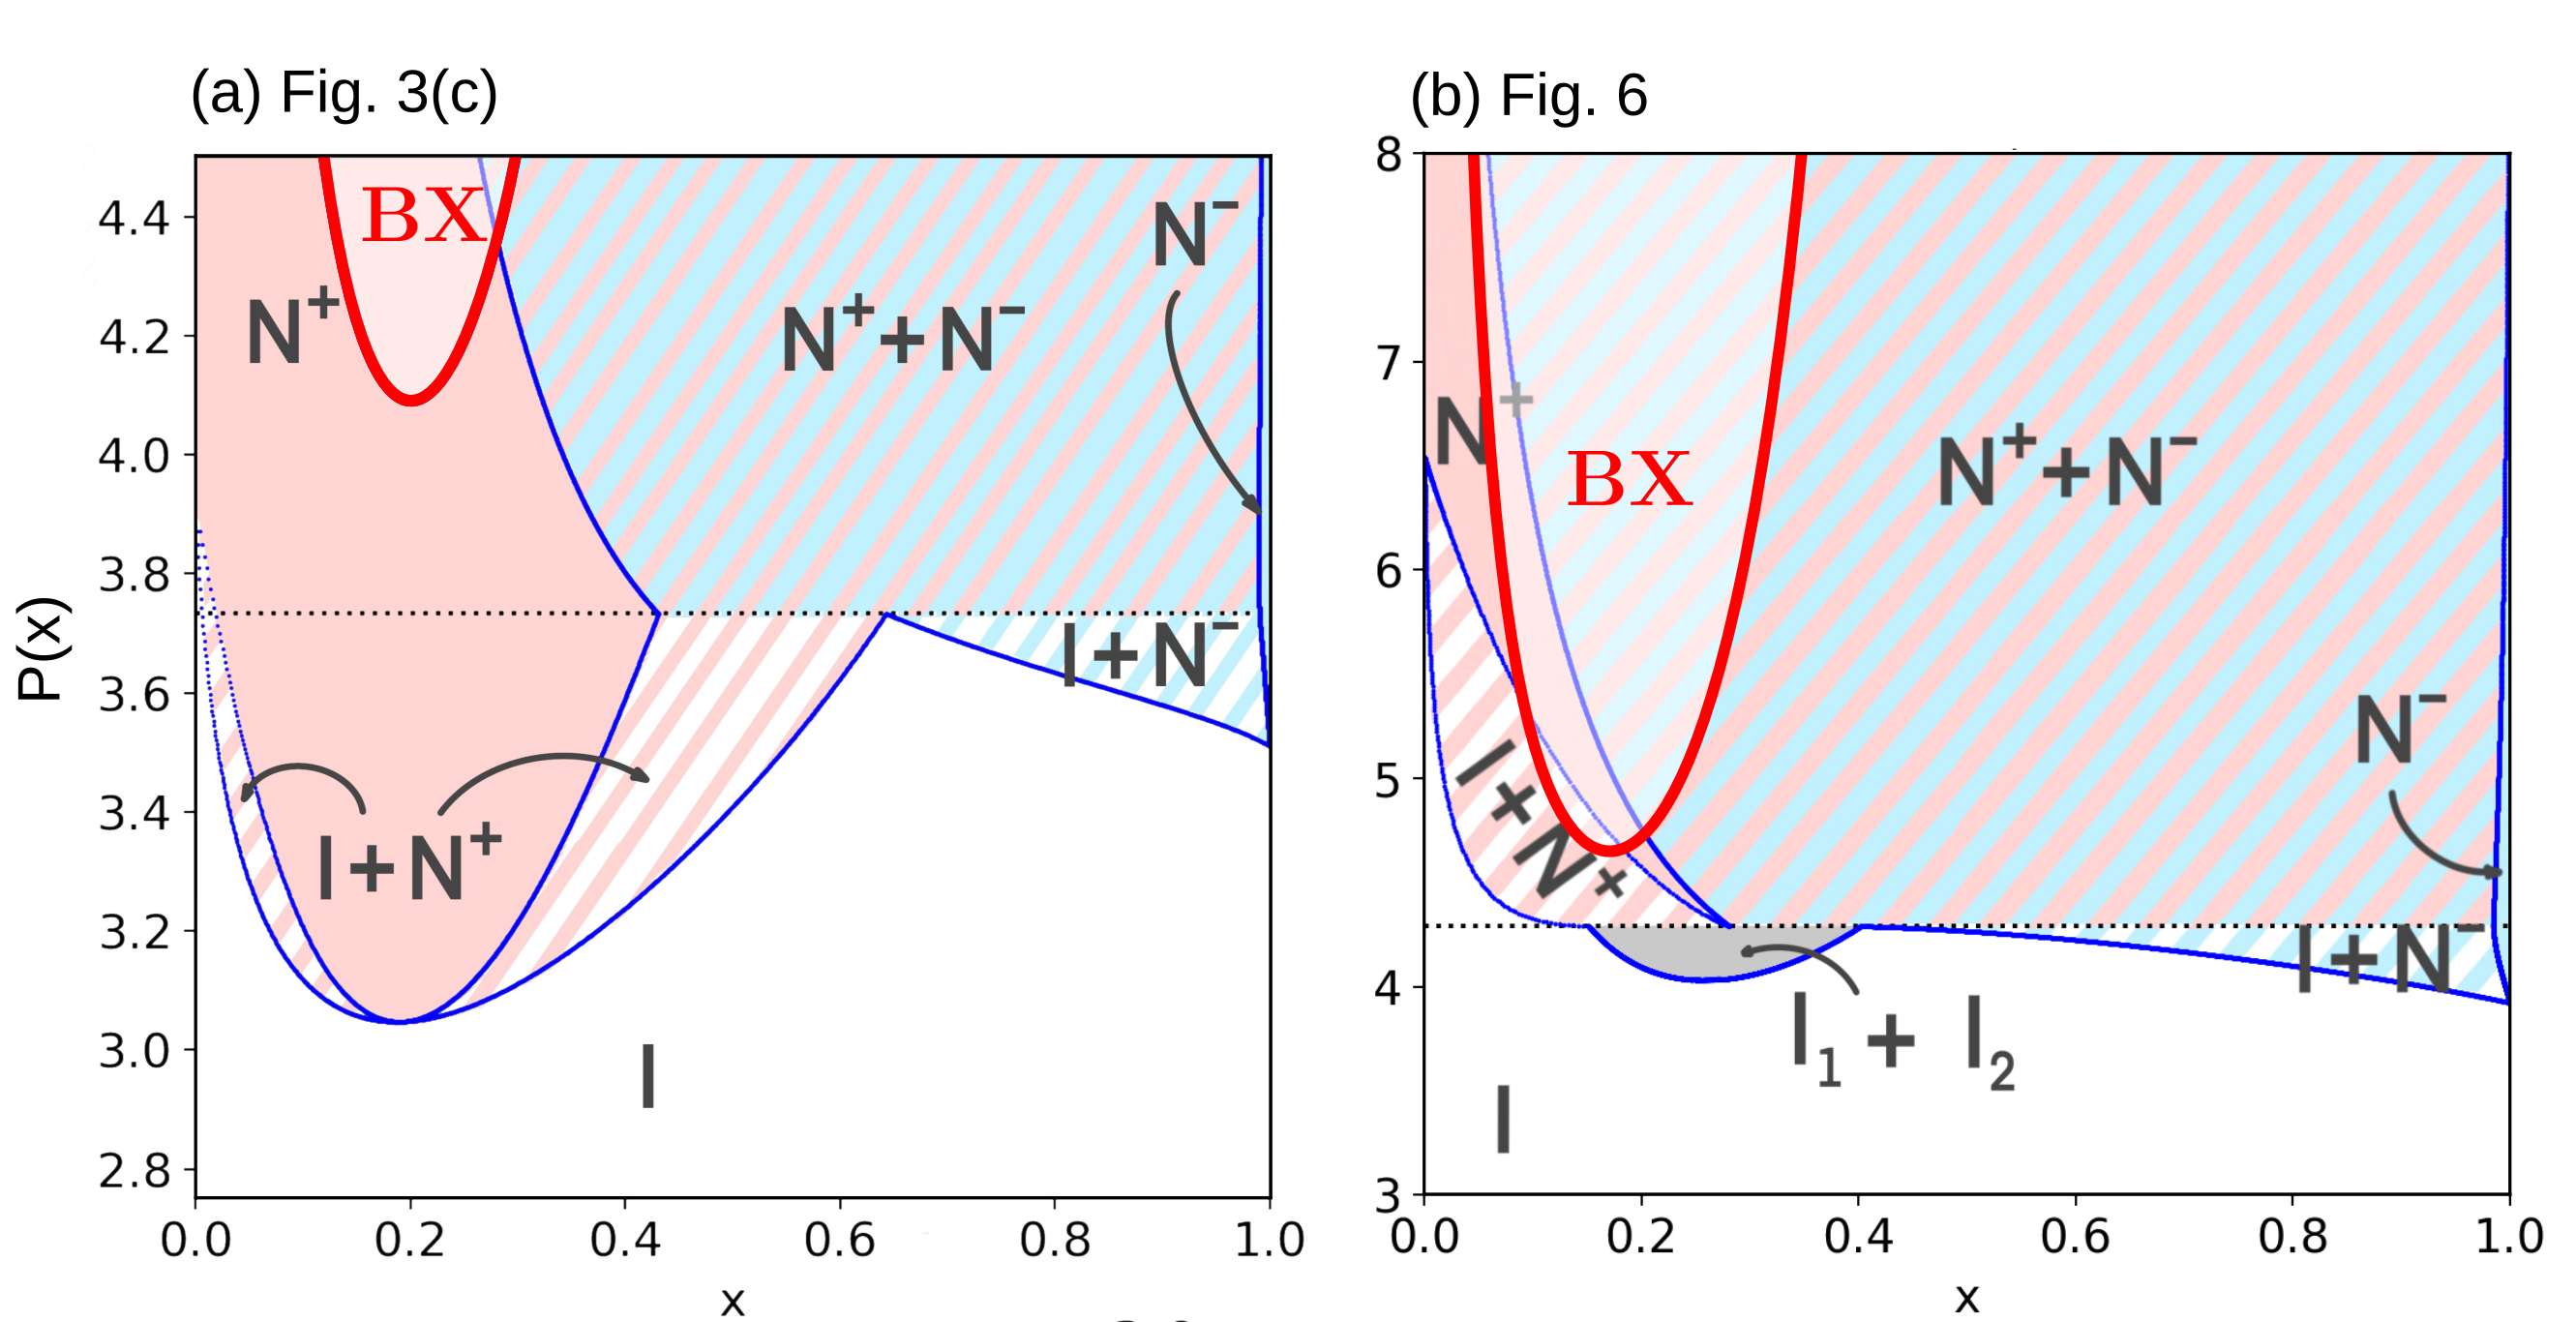
\includegraphics[width=.9 \textwidth]{figures/chapter-2/biaxial-altered}
\caption[Bifurcation curves superposed to their corresponding phase diagram]{ Bifurcation curves locating the transition from uniaxial (U) order at low osmotic pressure $P$ to biaxial (BX) nematic order at high pressure superposed to their corresponding situation discussed in the main text. (a) Case depicted in \fig{fig:L10}(c). (b) Case depicted in  \fig{fig:qp}  }
\label{fig:bx2}
\end{figure}

So far, we have overlooked the possibility of biaxial nematic order in which both polymers and discs order along mutually perpendicular directors (see \fig{fig:bx}(a)).
In order to tentatively locate the transition toward biaxial ($BX$) nematic order, we  apply a simple bifurcation analysis in which we probe the stability of a uniaxial ($U$) fluid against weakly biaxial fluctuations \cite{kayser,stroobants1984}. If the $U$-$BX$ transition is of second order, the bifurcation point at which biaxial solution emerges from the EL equations should pinpoint the actual phase transition.  We begin by generalizing the second-polynomial expansion \eq{p2expansion} to include biaxial nematic order using the addition theorem for spherical harmonics:
\begin{align}
\pp( \cos \gamma ) &= \pp(\cos \theta) \pp(\cos \theta^{\prime})  \nonumber \\ 
& + \frac{1}{12} \pp^{2}(\cos \theta) \pp^{2}(\cos \theta^{\prime}) \cos 2 (\varphi - \varphi^{\prime})
\end{align}
where $\varphi$ is the azimuthal angle describing the particle orientation  with respect to a secondary director $\bn_{\perp} \perp \bn$. The coupled EL equations then attain an additional term that accounts for biaxiality:
\begin{align}
&  \ell^{-1} \ln [  \rho_{r} (\ell, \oma ) \ell^{-1} ]   = \lambda_{r}    + \varepsilon_{b}  +  \alpha_{r}  \pp(\oma ) \nonumber \\ 
& +  \beta_{r } D(\oma)   +  \frac{L_{r}}{3\ell_{p}} \frac{\nabla^{2} [ \rho_{r} (\ell , \oma)]^{1/2}}{ [ \rho_{r} (\ell , \oma)]^{1/2} }
\label{lnrhorbiax}
\end{align}
and
\begin{align}
\ln [  \rho_{d} (\oma )] & = \lambda_{d}  + \alpha_{d} \pp(\oma)  + \beta_{d} D(\oma )  
\label{lndbiax}
\end{align}
in terms of the  weight function $D(\oma) = \sin^{2} \theta  \cos 2 \varphi $ and amplitudes: 
\begin{align}
\beta_{r} &=  \frac{15 }{16}  ( \rho_{r0} \bar{\Delta}_{r}  - 2q  \rho_{d0}  \Delta_{d} )  \nonumber \\
\beta_{d} &=   \frac{15 }{16}  (z \rho_{d0}  \Delta_{d}  - 2 q \rho_{r0}  \bar{\Delta}_{r} )
\label{alphabetabiax}
\end{align}
which feature the biaxial nematic order parameter of each species:
\begin{align}
\Delta_{r \ell} &= \rho_{r \ell}^{-1} \int d \oma \rho_{r}(\ell, \oma) D (\oma) \nonumber \\
\Delta_{d} &= \rho_{d0}^{-1} \int d \oma \rho_{d}( \oma) D (\oma ) 
\label{dr}
\end{align}
Similar to the uniaxial case the bar denotes a molecular-weight average according to $ \bar{\Delta}_{r} = \rho_{r0}^{-1}  \sum_{\ell} \rho_{r\ell} \Delta_{r \ell}$. 
Substituting the EL equations  into the  biaxial nematic order parameters and linearizing for weakly biaxial amplitudes $|\beta| \ll 1$ we establish the condition under which a biaxial solution for the orientation distribution bifurcates from the uniaxial  one:
\begin{align}
\Delta_{r \ell} &= \rho_{r \ell}^{-1} \ell \beta_{r} \int d \oma \rho_{r }^{(U)} ( \ell, \oma) D^{2} (\oma) \nonumber \\
\Delta_{d} &= \rho_{d0}^{-1}  \beta_{d} \int d \oma \rho_{d }^{(U)} (\oma) D^{2} (\oma)
\label{brod}
\end{align} 
This linear criterion basically stipulates the conditions (overall particle concentration, composition and effective temperature) at which the  uniaxial nematic state is no longer guaranteed to be a local minimum in the free energy. Within the factorization Ansatz \eq{pfac} for the uniaxial molecular-weight distributions the condition simplifies into:
\begin{align}
\bar{\Delta}_{r} &=  \beta_{r} (2 m-1)  \langle D^{2}  (\oma) \rangle_{f_{G}} \nonumber \\
\Delta_{d} &=   \beta_{d}  \langle D^{2}  (\oma) \rangle_{f_{G}}
\label{brodgauss}
\end{align} 
The brackets denote an average according to the nematic or anti-nematic Gaussians  $f_{G}$ specified in \eq{gaussians}. Similarly, $m$ denotes the mean aggregation number of either the $N^{+}$ or the $N^{-}$ phase.
The averages are easily obtained in the asymptotic angular limits ($\theta \ll 1$ or $\psi \ll 1$) and the leading order contributions read:
\beq
\langle D^{2}  (\oma) \rangle_{f_{G}}  \sim 
 \begin{cases}
 4 /[ \alpha^{(1)}]^{2} \hspace{0.5cm}  \textrm{nematic}  \\
1/2 \hspace{1.2cm}   \textrm{anti-nematic} 
\end{cases}
\eeq 
 The $U$-$BX$ bifurcation condition \eq{brodgauss} is equivalent to the matrix equation ${\bf M} \cdot {\bf \Delta}  = \lambda_{e} {\bf \Delta} $ with ${\bf \Delta} = ( \bar{\Delta}_{r} , \Delta_{d}) $ and ${\bf M}$ given by the prefactors.  The eigenvalues $\lambda_{e} $ of the matrix ${\bf M}$ are required to be unity $(\lambda_{e} =1)$. The solution is:
 \begin{align}
 1 &= -\frac{15}{32} c w_{1} \left[ (1-x) + xzW - \right . \nonumber \\ 
 & \left . \sqrt{(1-x)^{2} + 2Wx(1-x)(8 q^{2} -z) +W^{2} x^{2}z^{2} }  \right]
\end{align}
with
\beq
w_{1} = 
 \begin{cases}
 (2m_{N^{+}}-1) 4/\alpha_{r}^{2}  \hspace{0.5cm}  N^{+}-BX  \\
 (2m_{N^{-}}-1)/2 \hspace{0.7cm}  N^{-}-BX
\end{cases}
\eeq 
and
\beq
W = 
 \begin{cases}
 (2m_{N^{+}}-1)^{-1} \alpha_{r}^{2}/8  \hspace{0.5cm}  N^{+}-BX  \\
 (2m_{N^{-}}-1)^{-1} 8/\alpha_{d}^{2} \hspace{0.5cm}  N^{-}-BX
\end{cases}
\eeq 

The numerical solutions are shown in \fig{fig:bx}(b).  The $N^{-}$-$BX$ solutions ceases to be internally consistent with the Gaussian approximation at  $x< 0.8$ given that the nematic order parameter $\alpha_{d}$ of the discs tends to get too low. No such inconsistency occurs for the $N^{+}$-$BX$ branches. In general, we find that the transition occurs at pressures that are beyond the ranges explored in the phase diagrams of the main text. The only exceptions are \fig{fig:L10}(c) and \fig{fig:qp} where the $N^{+}$ phase remains stable up to fairly large disc mole fractions and the $N^{+}$-$BX$ bifurcations are located within the monophasic $N^{+}$ regions (in red), as shown in \fig{fig:bx2}. The tentative conclusion from this analysis is in line with previous reports in the literature \cite{mederos_overview2014}, namely that the stability of $BX$ nematic order is intimately linked to the excluded-volume asymmetry of the constituents which, in our case, is temperature-controlled.  Lowering the temperature reduces the typical asymmetry which then stabilizes well-mixed rod-disc nematics that subsequently may develop $BX$ order. We further note that disc-rich $BX$ phases seem much harder to stabilize than polymer-dominated ones as the $N^{-}$-$BX$ branches  generally do not intersect the small monophasic $N^{-}$ domains in the phase diagrams shown in the main text.


\end{subappendices}



\clearpage % Introduction II: MC simulations

\chapter{Emergent biaxial order in hybrid chiral LCs}
\chaptermark{Hybrid LCs: single-particle effects}
\label{hybridLC1}


\begin{abstract}
Cholesteric liquid crystals (LCs) are classic examples of complex chiral mesophases with long-ranged periodicity but lack positional order at large length scales. Doping molecular cholesterics LCs with thin colloidal rods or disks with a large  length-to-width ratio adds a further level of complexity due to the interplay between weak surface anchoring forces and elastic distortions around the rod-LC interface. We demonstrate that the rods have a strong tendency to orient perpendicular to the helix axis and local director, thus imparting strong local biaxiality on the hybrid cholesteric structure. We theoretically argue that the splay-bend elastic anisotropy plays a key role in stabilizing local orthorhombic order along the helix.  Our predictions are corroborated by experimental results obtained in the group of I. Smalyukh (University of Colorado, USA) that we briefly review. We also discuss the case of discs and find a similar scenario of anomalous biaxial order along the helical director for discs with homeotropic anchoring immersed in short-pitch cholesteric hosts LCs.


\end{abstract}



\section{Introduction}


Since the experimental discovery of chiral nematic liquid crystals (LCs) over 150 years ago \cite{planer1861notiz,reinitzer1888beitrage}, LC mesophases featuring chirality and long-range orientational order have been the focus of many research studies. The fundamental studies of geometry and topology of chiral nematic LCs as model systems provide extensive insights into physics principles associated with experimentally less accessible systems like particle physics or cosmology \cite{wu2022hopfions}, in addition to their technological application in electro-optics and displays. On the other hand, biaxial nematic mesophases have been highly sought-after in soft matter systems since their first theoretical consideration in 1970 \cite{freiser1970ordered}. However, even in a soft-matter system with strongly biaxial building blocks such as brick-shaped molecules, biaxiality was experimentally elusive and hard to unambiguously demonstrate in equilibrium states. Recent reports of the experimental discovery of biaxial nematic order include observations in micellar and molecular LCs formed by amphiphilic and bent-core molecules, respectively \cite{yu1980observation,tschierske2010biaxial}, and also colloidal dispersion of highly anisotropic particles immersed in molecular LC hosts, so-called hybrid nematics \cite{liu2016,mundoor2021,mundoor2018}.
The interplay between chirality and biaxiality in orientational order has been intensively studied for LC systems \cite{priest1974biaxial,kroin1989chirality,bunning1986effect,harris1997microscopic,dussi2016entropy,dhakal2011chirality,longa1994biaxiality,canevari2015biaxiality}. It has been concluded that cholesteric twisted alignment and biaxial order of LC molecules amplify each other and that a chiral twist configuration cannot be observed without building blocks featuring a certain degree of biaxiality in their orientational distributions at the molecular level. However, for purely molecular systems, the chirality-enhanced biaxiality of the molecular distribution was predicted and experimentally found to be rather weak \cite{priest1974biaxial,kroin1989chirality,bunning1986effect,harris1997microscopic,dussi2016entropy,dhakal2011chirality,longa1994biaxiality,canevari2015biaxiality}, scaling as $\ (qL_{\rm m})^2$ according to the prediction by Priest and Lubensky for single-component molecular LCs \cite{priest1974biaxial} (here $q=2\pi/p$, $p$ is the pitch of the chiral nematic and $L_m$ the molecular length). To date, to the best of our knowledge, there are no experimental or theoretical considerations of how the biaxiality of the orientational distribution of anisotropic colloidal particles could interplay with the chirality of the nematic host in hybrid molecular-colloidal LC systems.  



\begin{figure}
	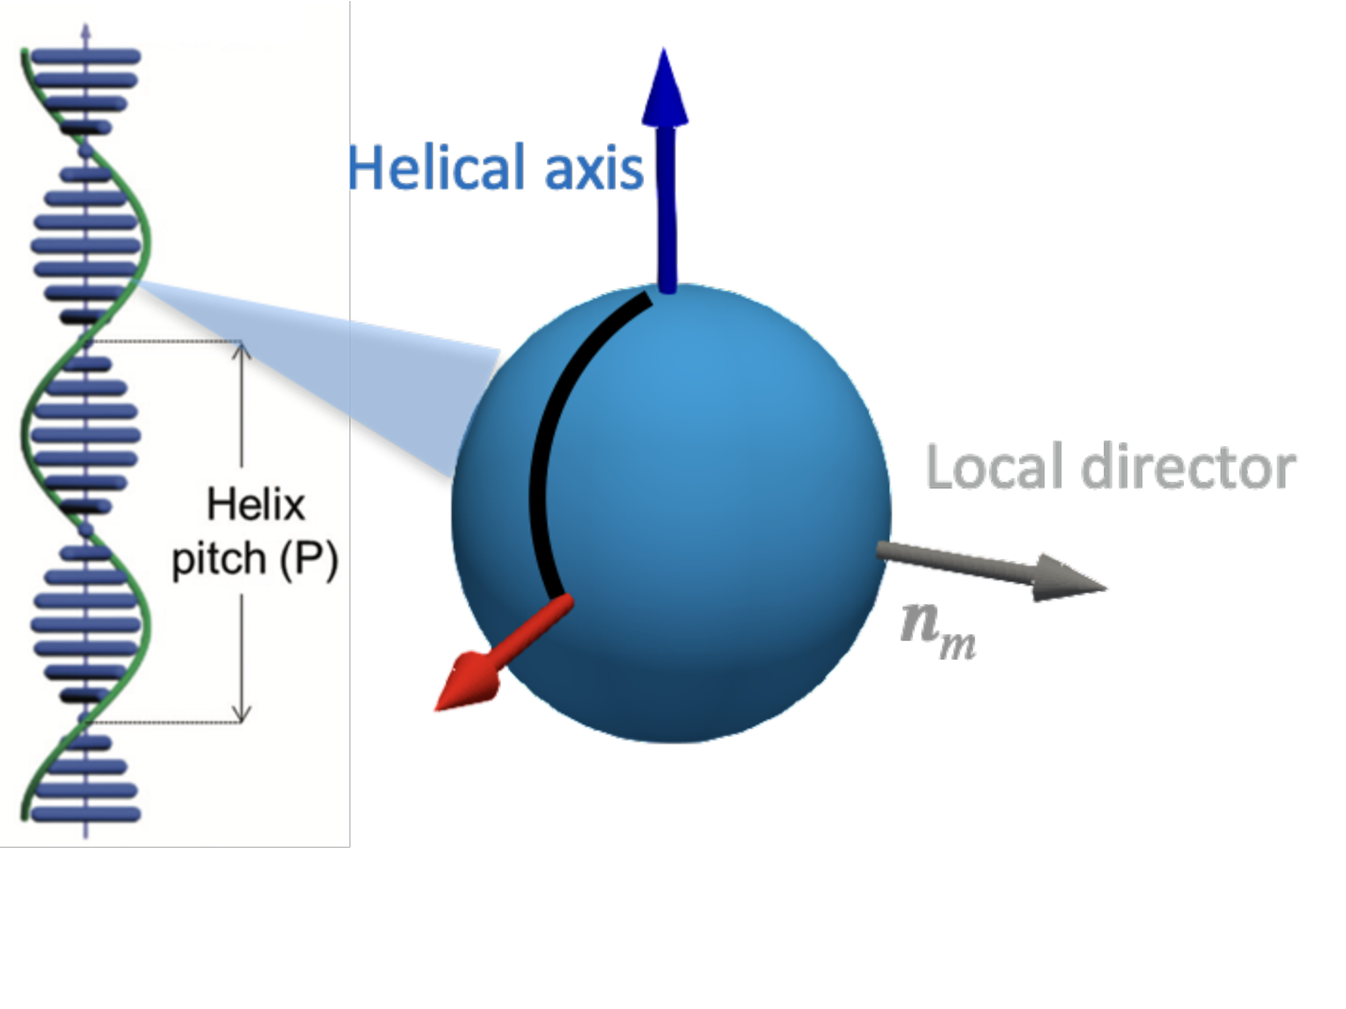
\includegraphics[width = 0.6 \columnwidth]{figures/chapter-3/tripod}
	\caption[Illustration of alignment opportunities for an anisotropic colloidal particles immersed in a cholesteric host LC.]{ Illustration of alignment opportunities for an anisotropic colloidal particles immersed in a cholesteric host LC. Depending on the surface anchoring properties of the colloid  and pitch of the cholesteric host, the colloid may  preferentially  align along either of the three main directions of the tripod.   Alignment along the red arrow leads to strong emergent local biaxial order of a hybrid colloidal-molecular LC.  }
	\label{tripod}
\end{figure}



In this chapter we present a theoretical survey of ordering properties of colloidal particles immersed in a low-molecular weight liquid crystal. Based on a simple mean-field theory that accounts for the surface anchoring energy of a single colloid we explore the alignment properties of thin elongated rods and flat discs with respect to the helical director field of the molecular host fluid 
(see \fig{twisdis}).  A key element is the preferred surface anchoring  properties of the molecular LC at the colloid surface which opens op several distinctly different ordering scenarios. Specific symmetries  that we explore  here are homeotropic, planar (see \fig{surfancho}) as well as conically degenerate surface anchoring for the case of discs.   Comparing with recent experimental results obtained in the group of I. Smalyukh (University of  Colorado, USA) we conclude that our theory accounts for most of the experimental observations, but for one case. We demonstrate that the alignment of rodlike colloid with homeotropic anchoring is not  driven by weak surface anchoring forces, but rather by a twisted surface disclination effects.  We address the weak elastic deformations around the colloids and demonstrate the twisted disclination wrapped around a thin rod  is the main driving forces between hometropic rods aligning perpendicular to the local host director and helical axis, thus imparting strong biaxial order onto the hybrid LC. A similar scenarios is envisaged for homeotropic discs, bit only in strongly cholesteric hosts with a pitch comparable to the disc diameter.




\section[Surface anchoring of a cylindrical rod]{Surface anchoring of a cylindrical rod immersed in a cholesteric host}


\begin{SCfigure}
	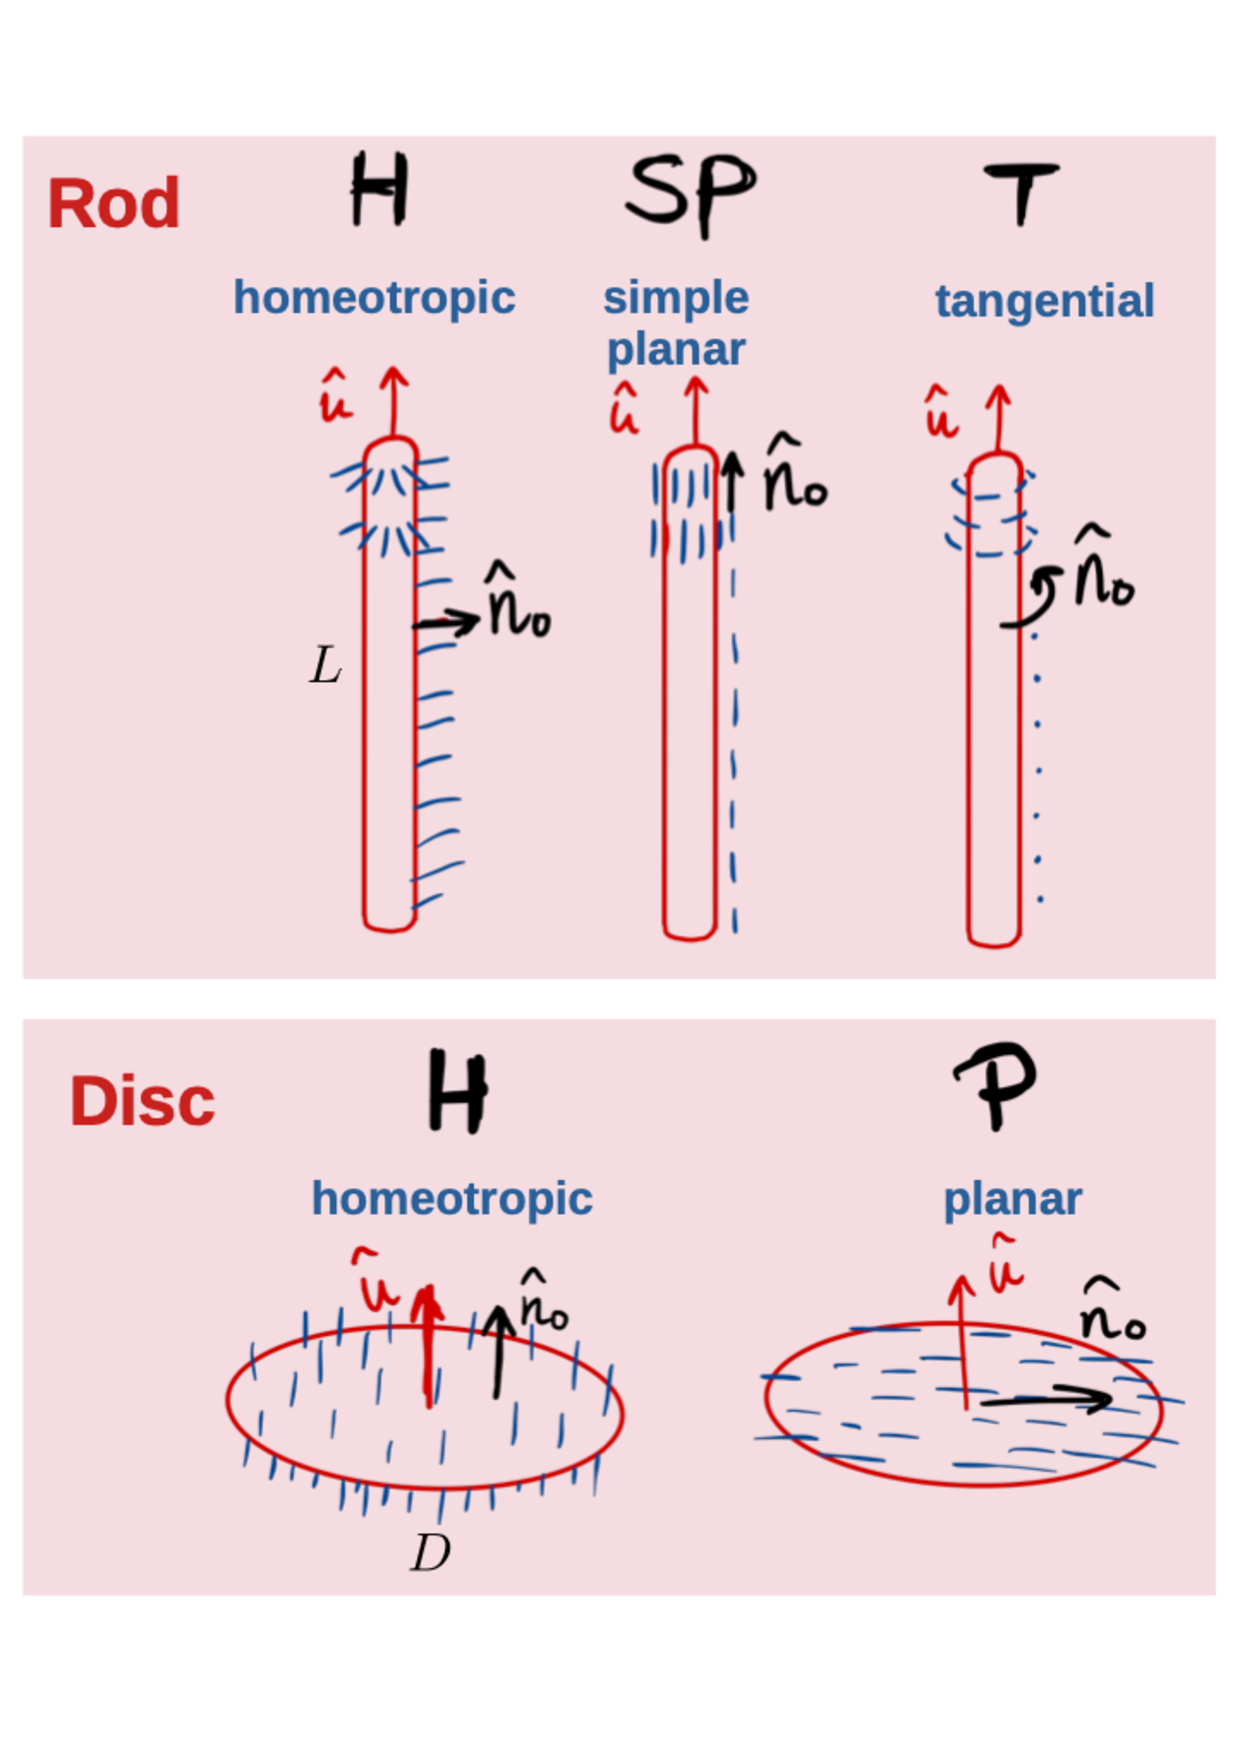
\includegraphics[width = 0.6 \columnwidth]{figures/chapter-3/surfanchoring}
	\caption{ Illustration of the different surface anchoring scenarios for a colloid rod with length $L$ (top) and disc with diameter $D$ (bottom).  }
	\label{surfancho}
\end{SCfigure}





Let us consider a low-molecular-weight chiral liquid crystal (such as 5CB with chiral dopants) with a director field $\bn(z)$ twisted along $Z$-axis of a Cartesian laboratory frame. The director field of the cholesteric solvent, denoted by ``$s$",  may be parameterized as:
\beq
\bn_{s}(z) = \bx \cos q Z  + \by \sin q Z
\label{ns}
\eeq
in terms of the pitch  $p = 2 \pi/q$ and handedness $q>0$ that we assume right-handed without loss of generality.
Next, we immerse a infinitely thin cylindrical rod with aspect ratio $L/D \rightarrow \infty$ into the chiral nematic  phase. The main axis of each rod can be parameterized as $\bhu = \bx \sin \theta \sin \varphi + \by \sin \theta \cos \varphi + \bz \cos \theta $ in terms of a polar $\theta$ and azimuthal angle $\varphi$ with respect to the helical axis $\bz$. The presence of the rod will generate elastic distortions of the uniform director field $\bn_{s}(\bfr)$ due to the specific anchoring of the molecules at the surface of the rod, quantified by  the surface anchoring energy  $W_{0}>0$ (units energy surface area). The extent of elastic deformation around the colloid surface ratio is commonly indicated by the surface extrapolation length $\ell_{s} = K/W_{0}$ where $K$ designates the typical elastic constant of the thermotropic liquid crystal.   In this project we focus on  the regime of large surface extrapolation length $ ( \ell_{s} \rightarrow \infty )$, in which case the elastic distortions are infinitesimally weak and the main energetic contribution imparted by the rod inclusions stems from the surface anchoring energy. Elastic corrections will be accounted for later on.   If we assume the molecular director field  $\bn$ to remain completely undistorted,  the surface anchoring free energy can be obtain from a simple Rapini-Papoular integral of \eq{ns} over the colloid surface denoted by ${\mathcal S}$:
\beq
F_{s} = -\frac{1}{2} W_{0} \oint d{\mathcal S}  (\bn_{s} \cdot \bn_{0}({\mathcal S}))^{2}
\label{rapo}
\eeq
with $\bn_{0}$ represent a unit vector normal to the colloid surface in case of {\em homeotropic} anchoring and tangential to the surface if the anchoring is {\em planar}.


For the particular case of a thin cylinder, we shall neglect small contributions associated with the ends of the cylinder so we only need to parameterize the cylindrical surface of magnitude $\pi LD$ following the principal contour $\bfr_{{\mathcal S}}(t) = \bfr_{0} +  \frac{L}{2}t\bhu $
with $-1<t<1$ of a cylinder with centre-of-mass $\bfr_{0}$. The surface anchoring free energy then becomes:
\beq
F_{s} = -\frac{1}{8} LDW_{0} \int_{0}^{2 \pi} d \phi  \int_{-1}^{1} dt  [ \bn_{s}( \bfr_{{\mathcal S}} \cdot {\bf \hat{z}}  ) \cdot \bn_{0} ]^{2}
\label{usurf}
\eeq
In order to describe various anchoring situations  we define two unit vectors $\bhe_{1,2}$ orthogonal to $\bhu$ and parameterize [Brochard-DeGennes]:
\beq
\bn_{0} = \begin{cases}
      \bhe_{1} \cos \phi + \bhe_{2} \sin \phi &  \textrm{H} \\
         -\bhe_{1} \sin \phi + \bhe_{2} \cos \phi &  \textrm{T} \\
      \bhu & \textrm{SP}
   \end{cases}
      \label{plahom}
\eeq
In the case of homeotropic (H) anchoring  the molecular director favors perpendicular alignment to the cylindrical surface, whereas  for tangential (T)  anchoring the easy axis follows the circular perimeter of the cylindrical cross section.
 The simple planar (SP) case corresponds to the easy axis $\bn_{0}$ pointing along main rod direction.    We obtain the following generic expression:
\begin{align}
 F_{s} = -\frac{\pi}{8} LDW_{0} \left ( w_{1} + w_{2} \cos (2 \delta )  \frac{\sin (qL \cos \theta)}{qL} \right )
 \label{us}
\end{align}
with $\delta = \varphi - q Z$ the azimuthal angle along a particle frame co-rotating with the  helical director so that $ \int d \bhu = \int_{0}^{2 \pi} d \delta \int_{-1}^{1}  d ( \cos \theta )$  and $w_{1}$ and $w_{2}$ are angle-dependent coefficients that depend on the particular anchoring situation:
\beq
w_{1} = \begin{cases}
      (1+ \cos^{2} \theta)  &  \textrm{H/T} \\
    2   \sin ^{2} \theta  & \textrm{SP}
   \end{cases}
      \label{w1}
\eeq
and
\beq
w_{2} = \begin{cases}
    -  \sin \theta \tan \theta    &  \textrm{H/T} \\
    2  \sin \theta \tan \theta   & \textrm{SP}
   \end{cases}
      \label{w2}
\eeq
in terms of the polar $\theta$ and azimuthal rod angle $\varphi$ with respect to the  helical axis. Note that the surface anchoring free energy is the same for the homeotropic and tangential anchoring scenarios.


For the homeotropic (H) case the free energy is minimal when  $\theta^{\ast} = 0$  (with the azimuthal angle $\varphi$ randomly distributed) which corresponds to the rod being  aligned along the helical axis. However, there is a second, degenerate minimum at $\theta^{\ast} = \pi/2$ and $\delta^{\ast} = \pi/2$, that describes a  rod pointing perpendicular both to the helical axis {\em  and} the local director.  The minimum surface anchoring energy is $F_{s} = -(\pi/4) LD W_{0}$ for both cases.  The energy barrier between the two minima is only about 0.2 $k_{B}T$ per rod so thermal fluctuations should easily make  the colloids switch from one state to the other.
 For simple planar (SP) anchoring we only find a single minimum at $\theta^{\ast} = \pi/2$ and $\delta^{\ast} = 0 $, i.e., the rod preferentially aligns along the revolving local nematic director.



\subsection{Non-interacting rods}

By balancing the surface anchoring free energy with the orientational entropy of the individual rods we easily establish the angular probability through the Boltzmann distribution:
  \beq
  f( \bhu ) = \mathcal{N} \exp (- \beta F_{s} (\delta, \theta)  )
  \label{fsingle}
  \eeq
 with $\beta^{-1} = k_{B}T$ the thermal energy in terms of temperature $T$ and Boltzmann's constant $k_{B}$ and $\mathcal{N}$ a normalization constant ensuring that $\int d \bhu f(\bhu) = 1$.  The surface anchoring strength is expressed  in dimensionless form by $\bar{w} = \beta LDW_{0}$.  The distributions are visualized in \fig{frod}.
It is easy to infer from \eq{us} that the polar and azimuthal angles are strongly coupled. This indicates that the local distribution of rod orientations around the principal alignment directions (blue, red or white arrow in \fig{frod}) is rendered {\em biaxial} by the chiral twist, as expected.  The most interesting situation arises for the H/T case where there is a subpopulation of  rods aligned along the helical axis ($qL=1$). In order to gain further insight into the orientational symmetry of those rods, we perform a small-angle expansion around   $\theta_{e} = 0$ and retain the leading order coupling term between the two principal angles $\theta$ and $\delta$. The angular fluctuations about the helical axis (blue) are then described by the following free energy
\beq
F_{s} \approx \frac{\pi}{8} LDW_{0}  j_{0}(qL) \cos (2 \delta) \theta^{2}
\label{ht_fluc_new}
\eeq
with $j_{0}(x) = \sin (x)/x$. It suggests that the subpopulation of rods aligned along the helical axis in fact adopt a {\em twist-bend}-type organization with a pitch $q$ identical to that of the molecular host. Contrary to cholesterics, these phases are characterized by a nematic director co-aligning with the helical axis. However, the situation here is more subtle given that  chirality is only manifested at the level of orientational fluctuations around a mean director ``backbone" that itself is not chiral.   We  identify a further interesting feature; depending on the sign of $j_{0}(qL)$ the twist-bend helix may be either in phase with the molecular helix ($\delta^{\ast} =0$ for  $qL=4$) or out-of-phase ($\delta^{\ast} = \pi/2$ for $qL=2$).


  \begin{figure}
	\includegraphics[width = 0.8\columnwidth]{figures/chapter-3/frod}
	\caption[Unit-sphere projections of the local orientational probability of a rod immersed in a low molecular-weight cholesteric]{ Unit-sphere projections of the local orientational probability of a rod immersed in a low molecular-weight cholesteric phase at different surface anchoring strengths $\bar{w} = \beta W_{0}LD$. Zones of high orientational probability are in red.  A bistable distribution is found for the homeotropic/tangential (H/T) anchoring case at elevated anchoring strength. For all distributions, the rod-length-to-pitch is $qL=1$. }
	\label{frod}
\end{figure}


%Finally, we may probe the possibility of {\em tetragonal} nematic order ($D_{4h}$) with four-fold symmetry across the plane perpendicular to the cholesteric director ${\bf \hat{n}}_{s}$. We propose the following order parameter:
%\beq
%\Delta_{4} = \langle (a^{2} - b^{2})^{2} - a^{2}b^{2} \rangle_{f_{q}}
%\eeq
%We may thus identify the local nematic symmetry of the colloids, namely  uniaxial  ($S \neq 0, \Delta = 0, \Delta_{4} =0$),  orthorhombic biaxial ($S \neq 0, \Delta \neq 0, \Delta_{4} \neq 0$) or tetragonal  ($S \neq 0, \Delta = 0, \Delta_{4} \neq 0$).
%}


\subsection{Non-interacting discs}

We may now explore the case of a  thin disc with $L \ll D$ immersed in a cholesteric LC. Let us denote its normal by $\bhu$ and ignore anchoring at the rim. Similar to the case of rods we  consider homeotropic (H) and planar (P)  anchoring symmetries that we may express as follows:
\beq
\bn_{0} = \begin{cases}
      \bhu & \textrm{H} \\
      \bhe_{1} \cos \xi + \bhe_{2} \sin \xi &  \textrm{P} \\
       \end{cases}
      \label{plahomm}
\eeq
The angle $0 < \xi < 2 \pi$ must be chosen randomly in the case when  planar anchoring is degenerate across all direction on the disc surface.
Ignoring finite-thickness effects for $L \ll D$ we parameterize the face of the disc  as follows:
\beq
\bfr_{{\mathcal S}} = \bfr_{0} + \frac{D}{2} t [\bhe_{1} \sin \phi + \bhe_{2}\cos \phi ]
\eeq
with $0< t <1 $ and $0 < \phi < 2 \pi$.
The surface anchoring energy per disc face is expressed analogous to \eq{usurf}:
\begin{align}
F_{s} &= -\frac{1}{4}  W_{0} D^{2} \int_{0}^{2 \pi} d \phi   \int_{0}^{1} dt t \int_{0}^{2 \pi} \frac{d \xi}{2 \pi} [ \bn_{s}( \bfr_{{\mathcal S}} \cdot {\bf z} ) \cdot \bn_{0} ]^{2}
\label{usurf2}
\end{align}
Leading to the following generic expression:
\begin{align}
 F_{s} = -\frac{\pi}{4}  W_{0}D^{2} \left ( w_{1} + w_{2} \cos (2 \delta ) \frac{J_{1}(qD | \sin \theta|)}{qD | \sin \theta| } \right )
 \label{usp}
\end{align}
with $J_{1}(x)$ a Bessel function of the first kind, $\delta = \varphi  - q z$ the  azimuthal angle with respect to the local cholesteric director, and coefficients:
\beq
w_{1} = \begin{cases}
    \frac{1}{2}  \sin ^{2} \theta    &  \textrm{H} \\
      \frac{1}{8}( 3 + \cos ( 2 \theta ))   & \textrm{P}
   \end{cases}
      \label{w1p}
\eeq
and
\beq
w_{2} = \begin{cases}
      \sin^{2} \theta    &  \textrm{H} \\
    -\frac{1}{2}  \sin^{2} \theta    & \textrm{P}
   \end{cases}
      \label{w2p}
\eeq
Similar to the rods the surface anchoring strength is expressed  in dimensionless form by $\bar{w} = \beta W_{0}D^{2}$. Taking discs with diameter $D \approx 2 \mu m$ and $W_{0} \approx 10^{-6} - 10^{-5} J/m^{2}$ we find an even higher value than for  the rods, namely  $\bar{w} \sim 10^{3}-10^{4}$ indicating that surface anchoring realignment is robust against thermal fluctuations.


   \begin{figure}
	\includegraphics[width = 0.8\columnwidth]{figures/chapter-3/fdisc}
	\caption[Unit-sphere projections of the local orientational probability of a disc immersed in a low molecular-weight cholesteric]{ Unit-sphere projections of the local orientational probability of a disc immersed in a low molecular-weight cholesteric phase at different surface anchoring strengths $\bar{w} = \beta W_{0}D^2$. For all distributions, the disc-diameter-to-pitch is $qD=1$. }
	\label{fd}
\end{figure}

\subsection{Conically degenerate surface anchoring}

The presented surface anchoring model is suitable for a vast selection of geometrical junctions between the cholesteric solvent and the particles. Another experimentally relevant scenario, and as a generalization of the previously evaluated situations, would consist of a preferred anchoring direction $\bn_{0}$ forming an angle $\alpha$ (and thus drawing a degenerate conical surface with apex angle $\alpha/2$) with respect to the vector normal to the colloid surface. Let $\xi$ be the integration angle around such a cone.

For rod-like particles, the anchoring free energy is expressed analogous to \eq{usurf}:
\begin{align}
F_{s} &= -\frac{1}{8} LDW_{0} \int_{0}^{2 \pi} d \phi   \int_{-1}^{1} dt \int_{0}^{2 \pi} \frac{d \xi}{2 \pi} [ \bn_{s}( \bfr_{{\mathcal S}} \cdot {\bf z} ) \cdot \bn_{0} ]^{2}
\end{align}
We may express $\bn_{0}$ in terms of the angles $\alpha$, $\phi$ and $\xi$:
 \begin{align}
\bn_{0} & = \bhe_{1}( \cos \phi \cos \alpha - \sin \phi \sin \alpha \cos \xi) \nonumber \\
       & + \bhe_{2} (\sin \phi \cos \alpha + \cos \phi \sin \alpha \cos \xi) \nonumber \\
       & + \bhu \sin \alpha \sin \xi
      \label{plahommm}
 \end{align}
Leading to an expression equivalent to \eq{us} with coefficients:
\beq
w_{1} =\frac{1}{2}(3 - \cos ^{2} \alpha + ( 3\cos ^{2} \alpha - 1 ) \cos ^{2} \theta )
\eeq
and
\beq
w_{2} = - \frac{1}{2}( 3\cos ^{2} \alpha - 1 ) \sin \theta \tan \theta
\eeq
We can similarly take \eq{usurf2} for discs. In this case we define $\bn_{0}$ as follows:
\beq
\bn_{0} = (\bhe_{1} \cos \xi + \bhe_{2} \sin \xi) \sin \alpha + \bhu \cos \alpha
      \label{plahommmm}
\eeq
Leading to an expression equivalent to \eq{usp} with coefficients:
\beq
w_{1} =\frac{1}{4}(2 - 2\cos ^{2} \alpha + ( 3\cos ^{2} \alpha - 1 ) \sin ^{2} \theta )
\eeq
and
\beq
w_{2} =\frac{1}{2}( 3\cos ^{2} \alpha - 1 ) \sin ^{2} \theta
\eeq
The corresponding distributions are given in \fig{heliconical}.

\begin{figure}
	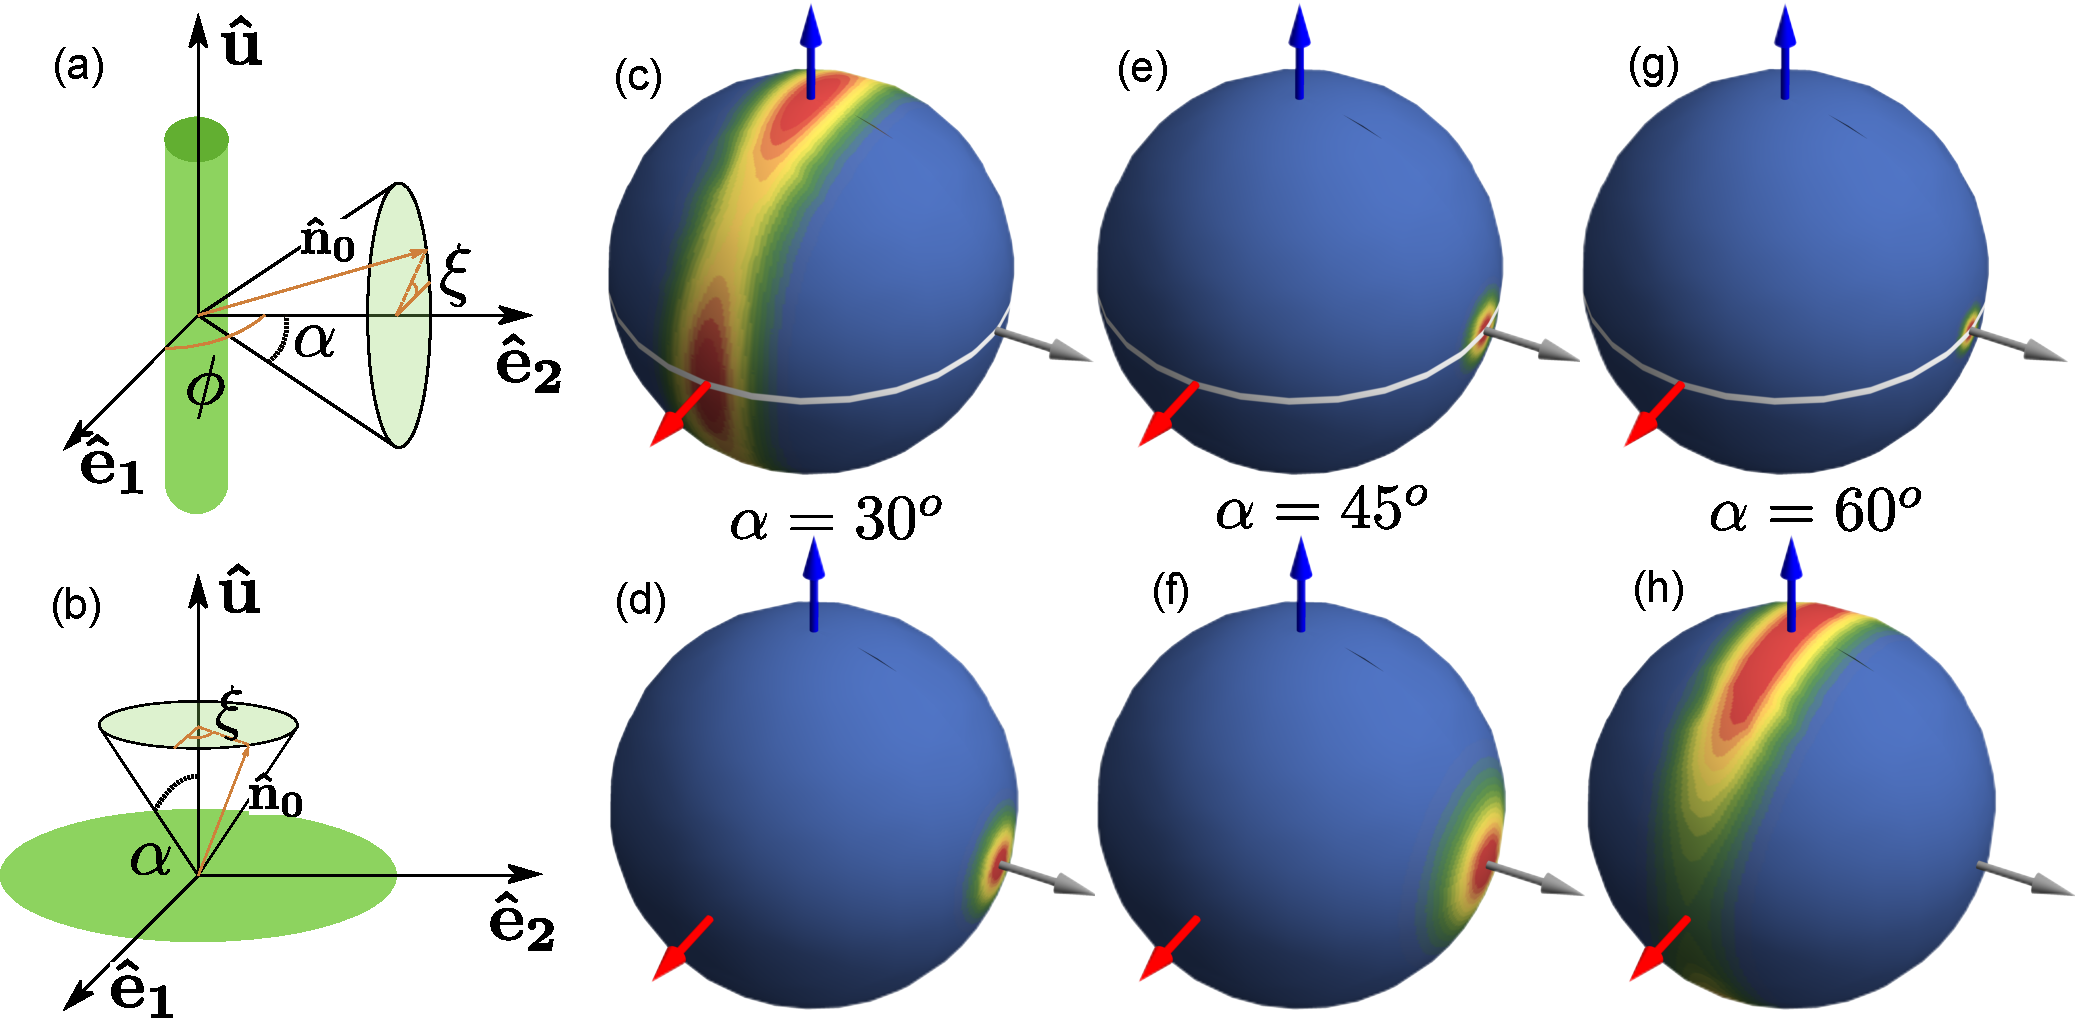
\includegraphics[width = \columnwidth]{figures/chapter-3/heliconical}
	\caption[Schemes to illustrate the conically degenerate surface anchoring]{ (a) (and (b)) Schemes to illustrate the conically degenerate surface anchoring with a fixed anchoring angle $\alpha$ on rods (and discs). (c-h) Unit-sphere projections of the local orientational probability of a rod (top panels c, e, g) or a disc (bottom panels d, f, h) immersed in a low molecular-weight cholesteric phase at different anchoring angles. For all distributions, the particle-length-to-pitch is $qL(D)=1$ and the surface anchoring strength is $\bar w = 100$. }
	\label{heliconical}
\end{figure}



\subsection{Order parameters}

In order to facilitate comparison with experimental results, we define orientational order  with respect to  $\bn_{s}$ which defines the principal direction of molecular alignment along the cholesteric helix. Taking the local host director $\bn_{s}$ as a reference we define a uniaxial order parameter:
\beq
S = \langle {\mathcal P}_{2} (\bhu \cdot \bn_{s})\rangle_{f_{q}}
\label{s2}
\eeq
A biaxial nematic order parameter measures the relative orientational order with respect to the principal directions orthogonal to $\bn_{s}$:
\beq
\Delta = \langle a^{2} - b^{2} \rangle_{f_{q}}
\label{d2}
\eeq
in terms of the projections $a= \bhu \cdot (\bn_{s} \times \bz)$ and $b = \bhu \cdot \bz$. We stress that this convention is by no means unique and one could also define orientational order from the tensor ${\bf Q}_{c} =  \frac{3}{2} \langle \bhu \otimes \bhu  \rangle_{f_{q}} - \frac{{\bf I}}{2} $ which measures the orientational order parameters ($S_{\rm c}$ and $\Delta_{\rm c}$) with respect to the principal colloidal alignment direction $\bn$, independent from the chosen reference frame.


\section[Model system]{Experimental model system}


The experiments performed in the group of I. Smalyukh are based on disk or rod-shaped $\beta- {\rm NaYF4:Yb/Er}$ particles are synthesized following the hydrothermal synthesis methods described in detail in Refs. \cite{mundoor2018,mundoor2021}. Homeotropic anchoring with 5CB (pentyl-cyanobiphenyl or 4-cyano-4'-pentylbiphenyl) molecules
on the $\beta-{\rm NaYF4:Yb/Er}$ disk surfaces is controlled
through surface-functionalization with a thin layer of
silica and polyethylene glycol.

The colloidal rods have length $L\approx 1.6 \mu m$, thickness $D \approx 25 nm$ and {\em homeotropic} (H) surface anchoring with amplitude $W_{0} \approx 10^{-5} J/m^{2}$. From this we find that $\bar{w} \approx 97$ indicating that the realigning forces generated by surface anchoring strongly exceed thermal fluctuation forces. The pitch of the cholesteric host is about $p \approx 30 \mu m $ so that $qL  \approx 0.335 $. The discs have a diameter of about $D \sim 2 \mu m $ and thickness of $L \sim 20 nm$. In view of their large diameter the surface anchoring amplitude $\bar{w} \sim 10^{3}-10^{4}$ each disk experiences strongly exceeds the thermal energy.  The results of the experiments are summarized in the table below. In additions, simulations have been performed based on numerically minmizing the Landau-DeGennes free energy around a colloidal particle immersed. The simulations fully account for the elastic anisotropy of the cholesteric host with input parameters based on the experimentally measured elastic moduli for 5CB. The surface anchoring amplitude and symmetry was varied in similar ways as in our theoretical approach.   Full details of the experiments and simulations will be disclosed in an upcoming joint publication with the group of I. Smalyukh. 



\begin{table}[h!]
\centering
    \begin{tabular}{|c||c c c c|} 
    \hline
    & $S$ & $\Delta$ & $S_{\rm{c}}$ & $\Delta_{\rm{c}}$ \\  
    \hline\hline
    homeotropic  disk &  0.6564 & 0.0673 & 0.6564 & 0.0673  \\ 
    \hline
    planar rod & 0.9360 & 0.0140 & 0.9360 & 0.0140   \\
    \hline
    homeotropic rod ($L = 1.7 \mu m$) &  -0.2561 & 0.7594 &  0.6976 & 0.1236  \\
    \hline
    homeotropic rod ($L = 3 \mu m$) & -0.3818 & 0.8935 & 0.8610 & 0.0650  \\
    \hline
    \end{tabular}
    \caption{Colloidal order parameters measured in the local molecular frame  and colloidal frame (with subscript `c') for each set of experiments. }
    \label{table_OPs}
\end{table}
From the measured order parameters  we infer that both  planar rods and hometropic discs both tend to align along the cholesteric director, whereas homeotropic rods strongly prefer to orient towards the perpendicular axis indicated in red in \fig{twisdis}. These obervations are in line with the distributions depicted in \fig{frod} for the rods and \fig{fd} for the discs. However, \fig{frod} suggests that hometropic rods with strong surface-anchoring coupling  $\bar{w} = 100 $ should  have an equal probability to the red and and blue arrows. This degeneracy is not observed in experiment where the subpopulation of rods pointing along the helix axis (blue) is estimated to be negligble. Clearly, the Rapini-Papoular surface anchoring energy does not suffice to explain the experimental observation which suggests that  elastic deformations incurred by the weak surface anchoring forces must play a subtle role.   This we will analyze next.


\section[Role of elastic distortions]{Comparison with experiments: role of elastic distortions}

In our analysis so far we have completely ignored elastic deformations of the host director ($\ell_{s} = K/W_{0} \rightarrow \infty$) so that rod realignment is dominated entirely by surface anchoring. The latter dictates that rods should point along the blue and red axis with equal probability (see \fig{frod}). The experimental reality, however, is that the surface anchoring extrapolation length is large but finite ($\ell_{s} \approx 600 nm \gg D$). Observations point at a scenario in which  rods  orienting along the red axis is largely preferred over the helical axis (blue). The reason why the latter is unfavorable  is that it involves a twisting of the surface disclination that runs along the rod contour which presumably costs energy. This is illustrated in \fig{twisdis}. No such twisting is necessary if the rod points along the red axis.   Clearly, the discrepancy between experiment and theory must be attributed to the  elastic distortions running along the rod surface (and their subsequent twisting) which was ignored in our model considerations thus far. In principle, weak director distortions may also lead to a minute decrease  of the bulk nematic order parameter,  in particular in regions where the director curvature is strong.  In our analysis, we will assume that the scalar order parameter of the host is preserved even close to the rod surface where director distortions are expected to be the strongest.



\subsection{Elastic energy of a twisted disclination wrapped around a thin rod}




\begin{figure}
	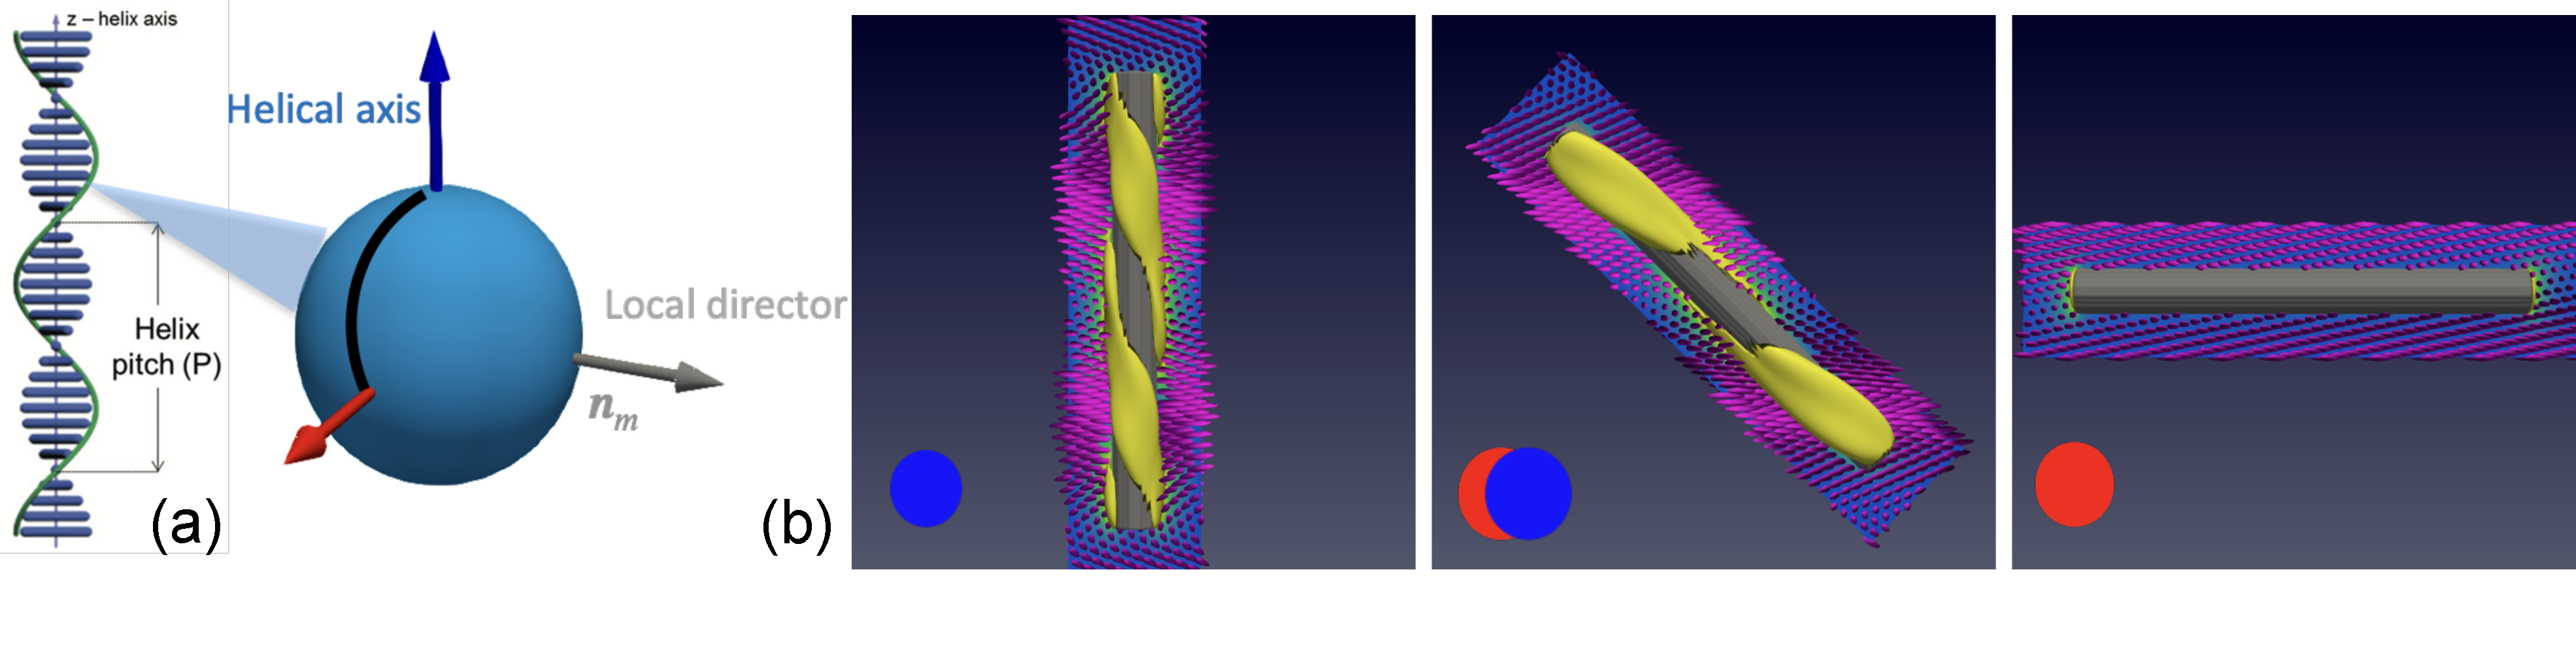
\includegraphics[width = \columnwidth]{figures/chapter-3/twisted_disclination}
	\caption[Illustrations of a helical surface defect emerging around a colloidal cylinder at various orientations]{ (a) Local tripod of directions along the molecular helix. (b) Illustrations of a helical surface defect emerging around a colloidal cylinder at various orientations along the tripod, indicated by the colored dots. When the rod align along the blue helix axis a helically twisted disclination occurs. It is absent when the rod points along the red arrow. Picture courtesy of Jason Wu (University of Colorado, USA). }
	\label{twisdis}
\end{figure}




We will now attempt to quantify the twisted disclination effect by introducing an angular deviation $\Phi(\bfr)$ and express the helical host director as follows:
\beq
\bn_{s}(\bfr) = \bx \cos( q z + \Phi(\bfr_{\perp}))  + \by \sin (q z + \Phi(\bfr_{\perp}))
\label{nsebluee}
\eeq
with $\bfr$ denoting a 3D distance vector and $\bfr_{\perp}$  the lateral distance perpendicular to the helical axis $\bz$.  The total free energy of a colloidal rod inclusion aligned along the helical axis is given by the Rapini-Papoular surface anchoring term \eq{rapo} combined with the Frank elastic free energy in the presence of chirality:
\begin{align}
F &= \frac{1}{2} \int d \bfr \left [ K_{1} (\nabla \cdot \bn_{s})^{2}  + K_{2} (\bn_{s} \cdot \nabla \times \bn_{s} + q)^{2} \right . \nonumber \\
& \left . +   K_{3} (\bn_{s} \times \nabla \times \bn_{s})^{2} \right ]
-\frac{1}{2} W_{0} \oint d{\mathcal S}  (\bn_{s} \cdot \bn_{0}({\mathcal S}))^{2}
\end{align}
with $K_{1}$, $K_{2}$ and $K_{3}$ respectively denoting the splay, twist and bend elastic modulus.  The saddle-splay term surface elasticity reads:
\beq
F_{se} = -\frac{K_{24}}{2} \oint d{\mathcal S} \cdot \left ( \bn_{s} \nabla \cdot \bn_{s} +  \bn_{s} \times \nabla \times \bn_{s}\right )
\eeq
and is expected to have very little impact in the current geometry (cf. spherical colloidal inclusion).
The director twist is very weak on the typical range of the director deformations which should be comparable to the rod diameter $D$ rather than the rod length $L \gg D$. For simplicity, we assume the rod to be infinitely long and elastic distortions to occur only along the radial direction $\bfr_{\perp}$ Employing cylindrical coordinates $\Phi(\bfr_{\perp}) = \Phi (r, \vartheta ) $, expanding up to second order in $q$ and integration over the  we obtain for the  free energy  $ F_{el}$ per unit rod length:
\begin{align}
 \frac{F_{el}}{L} &=  \frac{1}{2} \int d  \bfr_{\perp} \left \{ \frac{K_{1}}{r^{2}} (1+ \partial_{\vartheta} \Phi)^{2} + K_{3} (\partial_{r} \Phi)^{2} \right . \nonumber \\
  & \left . + \frac{(qL)^{2}}{12} \Delta K  \left  [ \frac{1}{r^{2}} (1+ \partial_{\vartheta} \Phi)^{2} - (\partial_{r} \Phi)^{2} \right ] \right \}
  \label{felo}
  \end{align}
  where $\Delta K = K_{3} - K_{1} >0 $ denotes the difference between the bend and splay moduli. The elastic anisotropy turns out to be of crucial importance since the twist correction $\mathcal{O}(q^{2})$  vanishes in case of the one-constant approximation $K_{1} = K_{3} = K_{2} = K$.
Similarly, the surface anchoring free energy reads up to quadratic order in $qL \ll 1$:
\beq
  \frac{F_{s}}{L} =  -\frac{W_{0}}{2} \oint_{\mathcal{C}} d %
\vartheta \left \{ \cos^{2}(\vartheta - \Phi)  - \frac{(qL)^{2}}{12} \cos [2 ( \vartheta - \Phi)]  \right \}   \eeq
where $\mathcal{C}$ denotes the circular contour of the rod cross section with diameter $D$.
For weak distortions $\Phi \ll 1$ we linearize for $\Phi$ and obtain:
\beq
  \frac{F_{s}}{L} \approx \frac{F_{s}^{(0)}}{L} -\frac{W_{0}}{2} (1- \tfrac{1}{6} (qL)^{2}) \oint_{\mathcal{C}} d  \vartheta   \sin 2 \vartheta  \Phi
  \label{fsdist}
\eeq
The first term is the contribution for the {\em undistorted} director field previously analysed:
\begin{align}
  F_{s}^{(0)} &=  -\frac{LW_{0}}{2} \oint_{\mathcal{C}} d %
\vartheta \left \{ \cos^{2}\vartheta - \frac{(qL)^{2}}{12} \cos 2  \vartheta \right \} \nonumber \\
& \sim -\frac{\pi}{4} W_{0} LD
\label{sabasis}
\end{align}
which corresponds to \eq{usurf} for a homeotropic rod aligned perpendicular to the helical axis ($\theta = \delta = \pi/2$) in the large pitch limit $qL \ll 1$. The second term in \eq{fsdist} accounts for the change of surface anchoring free energy generated by the elastic distortions.
The change of elastic free energy induced by the twist follows from:
\begin{align}
 \Delta F_{\rm twist}^{(el)}  &\approx  \frac{1}{24} (qL)^{2} L \Delta K   \mathcal{F} [ \Phi_{0} ]
\end{align}
where $\Phi_{0}$ denotes the distortion angle for the {\em untwisted} system, and:
\beq
 \mathcal{F} [ \Phi_{0} ]  = \int d \bfr_{\perp}  \left [ \frac{1}{r^{2}} (1+ \partial_{\vartheta} \Phi_{0})^{2} - (\partial_{r} \Phi_{0})^{2} \right ]
 \label{fmans}
\eeq
is a dimensionless quantity measuring the extent of the surface disclination surrounding the cylinder. Applying the one-constant approximation which does not lead to qualitative changes in this context, we determine $\Phi_{0}$ from minimizing:
\begin{align}
 \frac{F_{el}(q=0)}{KL} &=  \frac{1}{2} \int d \bfr_{\perp}  \left \{ \frac{1}{r^{2}} (1+ \partial_{\vartheta} \Phi)^{2} + (\partial_{r} \Phi)^{2} \right \}
\end{align}
so that $(\delta F_{el} / \delta \Phi )_{\Phi = \Phi_{0}} = 0$ and $\ell_{s}  = K/W_{0}$ defines the (finite) surface anchoring extrapolation length.  Functional minimization of the free energy we obtain the Laplace equation in polar coordinates:
\beq
\partial_{r}^{2} \Phi_{0} + \frac{1}{r} \partial_{r} \Phi_{0}  + \frac{1}{r^{2}} \partial_{\vartheta}^{2}\Phi_{0} =0
\label{lapo}
\eeq
subject to the boundary conditions:
\begin{align}
\Phi_{0}( \infty, \vartheta ) &= 0 \nonumber \\
 \ell_{s} \partial_{r} \Phi_{0}(D/2, \vartheta) &= \tfrac{1}{2} \sin 2 \vartheta
\label{phioo}
\end{align}
with the latter denoting a Neumann boundary condition at the colloid surface imparted by surface anchoring contribution  \eq{fsdist}.
The result is a simple dipolar field:
\beq
\Phi_{0}(r , \vartheta ) = -\frac{D}{16 \ell_{s}} \left ( \frac{D}{2r}   \right )^{2} \sin 2 \vartheta
\eeq
Plugging this back into \eq{fmans} and integrating we find that the difference in elastic energy between the twisted (blue) and untwisted (red) case in independent of the surface anchoring extrapolation length $\ell_{s}$ and increases logarithmically with system size $\ell_{\rm max}$:
\beq
 \Delta F_{\rm twist}^{(el)} \sim  \frac{2 \pi }{24} (qL)^{2} L \Delta K  \ln \left ( \frac{2 \ell_{\rm max}}{ D} \right )
 \label{twidi}
 \eeq
 Taking $\ell_{\rm max} = L$ as typical size cut-off, $\Delta K \approx 4 pN$ we find that $\Delta F_{\rm twist}  \approx 280 k_{B}T$.
 %For the total elastic free energy for a rod with untwisted distortions we find:
%\beq
%F_{el}(q=0) = \pi K L \left \{ \frac{D^{2}}{256\ell_{s}^{2}} + %\ln \left ( \frac{2 \ell_{\rm max}}{ D} \right ) \right \}
%\eeq
%which is about $3.5 \times 10^{4}$ $k_{B}T$.
The change in surface anchoring free energy associated with a twist of the director distortions reads:
\begin{align}
  \Delta F_{\rm twist}^{(s)} &
  \sim - \frac{\pi W_{0}LD}{92} \frac{D}{ \ell_{s}}  (qL)^{2}
\end{align}
which is  negligible compared to the elastic contribution above so that the total distortion-induced free energy change reads $\Delta F_{\rm twist} \approx \Delta F_{\rm twist}^{(el)}$.






\subsection{Elastic distortions around a rod tilted away from the host director}

In order to complete our understanding of the strength of the elastic distortions surrounding the main section of the rod we now look at the case where the rod remains perpendicular to the helix axis but makes an oblique angle with respect to the host director (see \fig{fel}). Ignoring chiral twist we parameterize the host director field case within a Cartesian reference frame with the rod aligned along $\bz$:
\begin{align}
\bn_{s}(\bfr) = & \begin{pmatrix}
\cos \Phi(\bfr)  \cos \chi(\bfr)\\
\sin  \Phi(\bfr) \cos \chi(\bfr) \\
 \sin \chi(\bfr)
 \end{pmatrix}
\label{nseblueee}
\end{align}
 As before,  we ignore end effects and and express the spatial variation of the distortion angles in polar coordinates, i.e. $\Phi(r , \vartheta)$ and $\chi(r, \theta )$. In principle, the  Euler-Lagrange expressions emerging from minimizing the elastic free energy are strongly coupled and cannot be solved analytically even in the case of weak surface anchoring. We expect, however, that a tilted rod will mostly experience distortions along its main axis $\bz$, expressed by a non-zero $\chi$, while the director deviations $\Phi$ surrounding the lateral cross-section of the rod remain far less affected by the rotation. Then, we can pursue a hybrid route by `constraining $\Phi = \Phi_{0}$ to its solution for the perpendicular case \eq{phioo} and minimize the free energy only with respect to $\chi$.
Working out the one-constant elastic free energy and taking the functional derivative we find that $\chi$ satisfies the following non-linear partial differential equation:
\begin{align}
\partial_{r}^{2} \chi + \frac{1}{r} \partial_{r} \chi  + \frac{1}{r^{2}} \partial_{\vartheta}^{2} \chi & = -\frac{\sin 2 \chi }{2r^{2}}
\label{nlpde}
\end{align}
Corrections to the right-hand term are of order $\mathcal{O}(1/r\ell_{s})$ and can be neglected for weak surface anchoring $\ell_{s} \gg D$.
In order to accommodate a rotation of the rod axis with respect to the far field host director we define a rotation matrix:
\beq
\mathcal{R}(\delta)  = \begin{pmatrix}
\sin \delta  & 0 & - \cos \delta \\
0 & 1 & 0 \\
\cos \delta & 0 & \sin \delta \\
\end{pmatrix}
\eeq
such that $\delta = \pi/2$ reverts to the case where the far-field host  director is perpendicular to the rod axis. The boundary conditions then follow from the Rapini-Papoular surface anchoring energy where the surface normal $\bn_{0}$ is subject to rotation:
\begin{align}
F_{s} &= -\frac{W_{0}}{2} \oint d{\mathcal S}  [\bn_{s} \cdot  (\mathcal{R} ( \delta ) \cdot  \bn_{0}({\mathcal S}))]^{2} \nonumber \\
& = -\frac{  W_{0} L}{2 } \oint d \vartheta \cos^{2} \vartheta \sin^{2}(\delta - \chi(D/2, \vartheta))
\label{raporot}
\end{align}
from which we infer that at $\delta = \pi/2$ (red arrow) optimal surface anchoring is achieved  when the  distortion angle $\chi $ is zero, which leads back to \eq{sabasis}. For oblique orientations $0<\delta < \pi/2$, severe distortions are generated since the optimal anchoring angle at the rod surface $\chi_{\rm surf} \sim \delta - \pi/2$ is incompatible with the far-field condition $\chi(r \rightarrow \infty) =0$.
The boundary condition for $\chi$ are the following:
\begin{align}
\chi(  \infty, \vartheta ) = & 0 \nonumber \\
\ell_{s} \partial_{r} \chi(D/2, \vartheta ) = & - \frac{1}{2 } \cos^{2} \vartheta \sin [2(\delta - \chi(D/2, \vartheta))] \nonumber \\
& + D^{-1} \sin 2 \chi(D/2, \vartheta)
\end{align}
The latter condition tells us that the distortions will be independent of the tilt angle $\delta$ at infinitely weak surface anchoring ($\ell_{s} \rightarrow \infty$), as we expect.
Clearly, the non-linear nature of the above differential equation and the complicated boundary conditions do not allow for an analytical solution of the problem.


\begin{figure}
	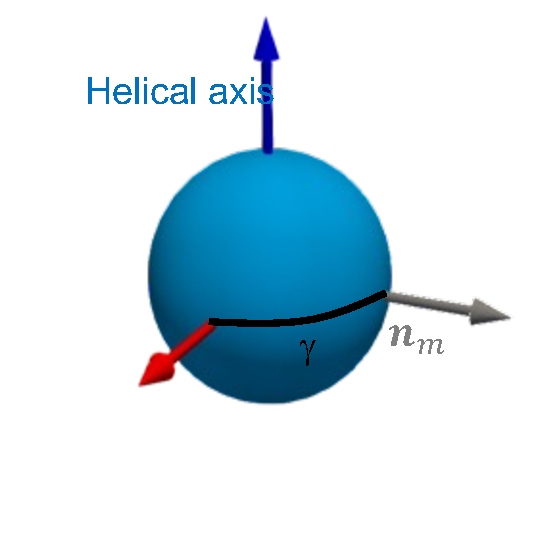
\includegraphics[width = .3\columnwidth]{figures/chapter-3/gamrods}
 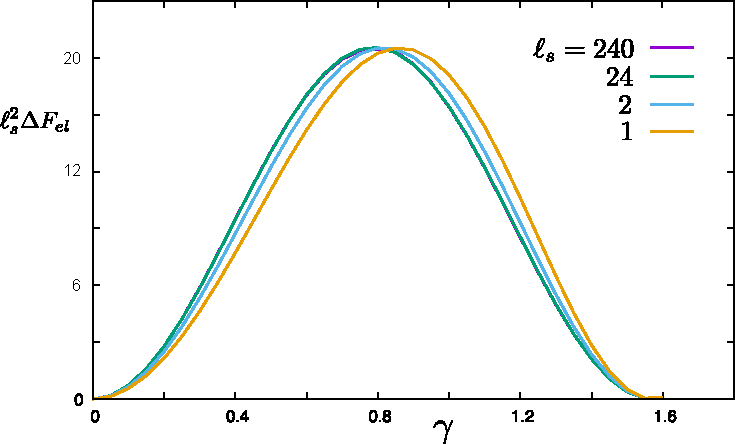
\includegraphics[width = .6\columnwidth]{figures/chapter-3/fel}
	\caption[Free energy associated with elastic distortions around a homeotropic rod tilted at an angle $\gamma$]{Free energy associated with elastic distortions around a homeotropic rod tilted at an angle $\gamma$ away from the red arrow towards the molecular director (grey) at different surface anchoring extrapolation lengths $\ell_{s}$ (expressed in units of the rod diameter $D$).   }
	\label{fel}
\end{figure}




\subsubsection{Curvature-free rod cross-section}

A more tractable  way forward is to transform the above expressions into a Cartesian coordinate system, so that $\chi(x,y)$ with the far-field host director pointing along the $x$-axis. Basically, we  assume that the rod cross-section along which the director distortions are expected to occur can be described by a strip of length $L$ and $D \ll L$. Further, we define a tilt angle $\gamma = \delta - \frac{\pi}{2}$ (with $0<\gamma <\pi/2$) so that $\gamma =0$ corresponds to the most favorable case where the rod points perpendicular along the red arrow.  All distances are normalized in terms of $D$. The distortions are then described by the 2D Laplacian:
\beq
(\partial_{x}^{2} + \partial_{y}^{2}) \chi  = 0
\eeq
of which the general solution reads:
\beq
\chi(x,y) = \sum_{n=1}^{\infty} e^{-n \pi x } [ a_{n} \cos(n \pi y) + b_{n} \sin( n \pi y ) ]
\label{seriesxy}
\eeq
which vanishes in the far-field limit $\chi(x \rightarrow \infty) = 0$. The (Rapini-Papoular) surface anchoring free energy reads:
\begin{align}
\frac{F_{s}}{KL} = - \frac{1}{2 \ell_{s}} \int_{0}^{1} dy \cos^{2} (\gamma - \chi(0,y))
\end{align}
which translates into the following boundary condition at the surface of the strip located at $x=0$:
\beq
\ell_{s} \partial_{x} \chi(0,y) = \frac{1}{2 } \sin [ 2 (\gamma - \chi(0,y)) ]
\label{bcweak}
\eeq
Further, for symmetry reasons we require the distortion angle to be vanishing at both sides of the strip:
\beq
\chi(0, 0 ) = \chi(0, 1)  =0
\eeq
which implies that $a_{n} =0$. The coefficients $b_{n}$ need to be  resolved from:
\beq
n \pi b_{n} = \frac{1}{ \ell_{s}} \int_{0}^{1} dy \sin (n \pi y) \sin \left [ 2 \left (\gamma - \sum_{k=1}^{\infty} b_{k} \sin (k \pi y) \right ) \right ]
\label{bcnum}
\eeq
For small tilt angles $\gamma  \ll 1$  distortions are expected to be weak $\chi \ll 1$ so that we linearize $\sin 2 (\gamma - \chi ) \approx 2( \gamma  - \chi)$.
This enables us to resolve the coefficients analytically:
\beq
b_{n} =  \left ( \frac{1 - (-1)^{n}}{(n \pi)^{2}}\right ) \frac{\gamma}{\ell_{s}}
\eeq
The free energy increase induced by the elastic distortions is given by:
\begin{align}
\Delta F_{el} &= \frac{ \pi KL}{4} \sum_{n=1}^{\infty} n b_{n}^{2}
\label{dfelseries}
\end{align}
which in the linearized regime for small $\gamma$ gives a simple analytical result:
\begin{align}
\Delta F_{el} = \frac{7 KL}{8 \pi^{3}} \zeta(3) \left ( \frac{\gamma }{\ell_{s}} \right )^{2}
\label{felgg}
\end{align}
with $\zeta(3) \approx 1.2 $ a constant from the Riemann-Zeta function $\zeta(x)$. The surface anchoring free energy reads:
\begin{align}
F_{s} = - LDW_{0} \int_{0}^{1} dy \cos^{2} (\gamma - \chi(0,y))
\end{align}
Then, in the absence of elastic distortions and no tilt ($\gamma = 0$) the surface anchoring free energy would simply be $F_{s} = -LDW_{0}$ which only marginally differs from the result for the cylindrical case $F_{s} = -(\pi/4)LDW_{0}$.
Within the linearized regime for small tilt angles $\gamma \ll 1$  the change in surface anchoring free energy imparted by the elastic distortions is given by:
\begin{align}
\Delta F_{s} &\approx LDW_{0}  \int_{0}^{1} dy  (\gamma - \chi(0,y))^{2}  \nonumber \\
& \approx W_{0} LD  \left ( 1 + \frac{1}{48 \ell_{s}^{2}} - \frac{7  \zeta(3)}{ \pi^{3} \ell_{S}} \right) \gamma^{2}
\end{align}
This expression along with \eq{felgg} clearly reflects the basic trade-off between surface anchoring and elasticity in which the cost in elastic free energy is in part compensated by a reduction of the surface anchoring free energy (last term). The total free energy change for small tilt angles now reads:
\beq
\Delta  F_{\rm tot} \sim  W_{0} LD \left ( 1  - \frac{49 \zeta(3)}{8\pi^{3} \ell_{s}}  \right ) \gamma^{2} + \mathcal{O}(\gamma^{2}/\ell_{s}^{2})
\label{ftiltcorr}
\eeq
Let us now compare our results with the simple Rapini-Papoular expression \eq{usurf} in the {\em absence} of elastic distortions. Taking $\theta=\pi/2$ and expanding for small $\gamma $ we find:
 \beq
 \Delta  F_{\rm tot}^{(RP)} \sim \frac{\pi}{4} W_{0}LD \gamma^{2}
\eeq
Disregarding the trivial curvature prefactor $\pi/4$ in the last expression, we find that the impact of the elastic distortions is rather marginal, since the correction term in  \eq{ftiltcorr} is less than 1 $k_{B}T$. Numerical resolution of \eq{bcnum} reveals that weak elastic distortions  occur mostly when the rod is at an oblique angle $\gamma = \pi/4$.
This is illustrated in \fig{fel} for a number of different anchoring strengths expressed by the extrapolation length $\ell_{s}$.

Now that we have established that distortions remain weak at any angle $\gamma$ for large enough extrapolation length $\ell_{s}  \gg 1$ we may explore an alternative route to quantifying $\chi$ by linearizing the boundary condition \eq{bcweak} for $\chi \ll 1$:
\beq
\ell_{s} \partial_{x} \chi(0,y)\approx \frac{1}{2 } \sin ( 2 \gamma) - \chi(0,y) \cos (2 \gamma )
\label{bcweak}
\eeq
From which the coefficients are easily established:
\beq
b_{n}  = \frac{\sin ( 2 \gamma )}{\cos(2 \gamma) - n \pi \ell_{s}} \left ( \frac{1-(-1)^{n}}{n \pi}\right )
\eeq
The corresponding elastic free energy then follows from the summation in \eq{dfelseries} and the results agree with the ones shown in \fig{fel}.







\subsection{Effective orientational potential of a LC rod}

Gathering the findings of the previous paragraphs we revisit the realigning potential acting on each rod. The total external potential is given by the bare Rapini-Papoular contribution \eq{usurf} for the undistorted host director plus the free energy contributions from elastic distortions:
\beq
U_{\rm rod} (\theta, \delta) \sim  F_{s}(\theta, \delta)  + \Delta F_{\rm dist}(\theta, \delta)
\eeq
Since the distortion term cannot be resolved for any rod orientation but only for cases when the rod is aligned along the principal Cartesian axes of the host frame we use the following interpolation form:
\begin{align}
\Delta F_{\rm dist} (\theta, \delta)  \sim & \Delta F_{\rm twist} \cos^{2} \theta  + \Delta F_{\rm tilt} \sin^{2} \theta \cos^{2} \delta
\end{align}
in terms of the two principal elastic  contributions;  $\Delta F_{\rm tilt} = F(\textrm{grey}) - F(\textrm{red})$ associated with tilting  the rod away from the red arrow and $\Delta F_{\rm twist}$ [\eq{twidi}] the energy cost associated with twisting of the surface disclination wrapped along the main part of the cylinder. From the analysis in the previous paragraphs we  found that $\Delta F_{\rm twist} = \mathcal{O}(10^{2} k_{B}T)$ whereas elastic distortions due to tilting are very weak $\Delta F_{\rm tilt} < k_{B}T$ and may, in fact, be neglected all together for the weak anchoring regime.  The  elastic energy is minimal (zero) when the rods align along the red arrow ($\theta = \pi/2$ and $ \delta= \pi/2 $) as observed in experiment.

At infinitely low rod concentrations, the order parameters $S$ and $\Delta$ defined within the frame of the  molecular host (\eq{s2} and \eq{d2}) are readily computed from the Boltzmann factor
  $f( \bhu ) = \mathcal{N} \exp ( - \beta  U_{\rm rod} (\delta, \theta)   ) $.
An overview of the results as a function of the anchoring strength $\bar{w} = \beta W_{0} LD$ is given in \fig{ww}. The best correspondence with experimental data for homeotropic rods listed in Table 3.1 is found for $ \bar{w} \sim 6 k_{B}T$ which corresponds to a surface anchoring  amplitude of about $W_{0}\sim 6 \times 10^{-7} J/m^{2}$.


\begin{figure}
	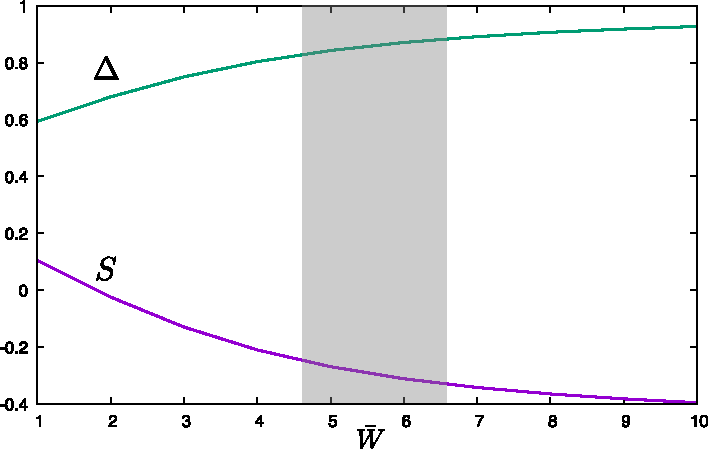
\includegraphics[width = .8\columnwidth]{figures/chapter-3/wwmans}
	\caption[Colloidal nematic order parameters measured within the molecular frame as a function of
the surface anchoring]{ Colloidal nematic order parameters measured within the molecular frame as a function of
the surface anchoring amplitude $\bar{w} = W_{0}LD$. The experimentally relevant region is indicated in grey. }
	\label{ww}
\end{figure}



The typical energy scale related to the twisted disclination effect can be gleaned from the the orientational distribution of the colloidal particles that have been measured in experiment.  From these, we can identify a standard Gaussian ${\rm FWHM} =2.355/\sqrt{2 \Delta F_{\rm twist}}$. This subsequently gives $\Delta F_{\rm twist} \approx 22 k_{B}T$ for homeotropic rods with  $L  = 1.7 \mu m $  and $\Delta F_{\rm twist} \approx 76 k_{B}T$  for the longer rods  with $L  = 3 \mu m $ suggesting that, in both cases, the thermal motion of the rods is assuredly insufficient to overcome the energy barrier between the $\tau$ and $\chi$ alignment directions. The values are in qualitative agreement with the prediction from our analytical model \eq{twidi} where $\Delta F_{\rm twist} \propto L^{3}$ suggests the energy to indeed be quite sensitive to the colloidal rod length. The actual values from  \eq{twidi}, however, should be considered as an upper bound for $\Delta F_{\rm twist}$ mainly because in our model the local nematic order parameter of the host is constrained at its far-field bulk value and is not allowed to relax in regions where director distortions are the largest, as observed in the experiment and simulations. 








\subsection{Short-pitch cholesteric hosts}


 At much short pitches,  comparable to the disc diameter, fluctuations in $\delta$ are greatly facilitated and the local minimum of $U_{\rm disc}$ eventually switches over to $\delta = \pi/2$ suggesting  discs  preferentially aligning perpendicular to the director and helical axis.  Taking the Rapini-Papoular contribution \eq{usp} as the main contribution for the weak surface anchoring regimes considered here we can extract  nematic order parameters associated with such a crossover.  The results, shown in \fig{disop}, clearly exhibit a sharp transition from uniaxial to biaxial order at a critical pitch of about $qD \approx 3.8$ which, taking $D =2 \mu m$ would correspond to cholesteric pitch of about $p \approx 3.3 \mu m$.



\begin{figure}
	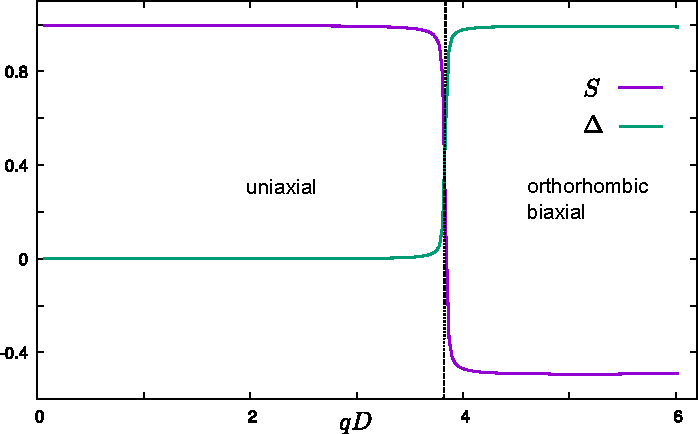
\includegraphics[width =  .8\columnwidth]{figures/chapter-3/discubx}
	\caption[Nematic order parameters of discs with weakly homeotropic surface anchoring immersed in a cholesteric host]{Nematic order parameters of discs with weakly homeotropic surface anchoring immersed in a cholesteric host with variable pitch $qD$. A crossover from uniaxial to orthorhombic biaxial local order occurs at around $qD \approx 3.8$.  }
	\label{disop}
\end{figure}



\subsection{Elastic distortions around a disc}

Ignoring elastic distortions we find that discs with homeotropic surface anchoring tend to orient along the grey axis, as observed in experiment (see Table 3.1). This is the obvious optimal situation that incurs the least amount of elastic distortions, compared to the other principal directions in which cases the disc surface would experience strongly unfavorable tangential surface ordering. However, even when the disc normal is aligned along the local nematic director  there are, however, local mismatches between the far-field and preferred surface director due to the weak twisting of the host director perpendicular to the disc normal (which occurs along the red axis) and when the rod normal fluctuates away from this axis. The elastic distortions are expected to be weak but they will become more outspoken at shorter pitches.  It is instructive to compute the extent of these distortions along the lines of our previous analysis for rods. Let us consider an infinitely thin disc with its normal restricted to lie in the $xy$-plane at an angle $\delta$ away from the optimal direction indicated by the grey arrow ($x$-axis). The principal directions are indicated by the tripod in \fig{discel} with the $xy$-plane corresponding to the one spanned by the red and grey arrows. We assume weak elastic distortions $\chi$  developing in the $xy$-plane.  Defining a host director $\bn_{s} = (\cos \Phi(x,y),
\sin \Phi(x,y) , 0)$ we find,  assuming  elastic isotropy,  that the distortions are described by the Laplace equation:
\beq
(\partial_{x}^{2} + \partial_{y}^{2}) \Phi  = 0
\eeq
The effect of a twisting host director is accounted for in the surface anchoring free energy:
\begin{align}
F_{s} &=  -\frac{W_{0}}{2} \oint d{\mathcal S}  [\bn_{s} \cdot  (\mathcal{R} (qz + \psi) \cdot  \bn_{0}({\mathcal S}))]^{2}
\label{raporotdisc}
\end{align}
where ${\mathcal S} $ parameterizes the face of the disc (as previously we ignore finite thickness effects for discs with $D \gg L$) and $\bn_{0} = (1,0,0)$ indicating homeotropic anchoring along the surface normal. The rotation matrix reads:
\beq
\mathcal{R}( qz )  = \begin{pmatrix}
\cos qz  & -\sin qz  & 0 \\
\sin qz & \cos qz & 0 \\
0 & 0 & 1 \\
\end{pmatrix}
\eeq
A key distinction with the rod case is that the distortions are not uniform across the disc surface but depend on the location of the surface element with respect to the helical axis.  It is convenient to divide the disc surface into infinitely thin strips, with each surface element on the strip being equidistant from the centre-of-mass along the twist direction ($z$-axis) thus experiencing the same degree of elastic distortions.

For notational brevity, we implicitly normalize all lengths in units of the disc diameter $D$ and parameterize the disc surface in terms of $y = \tfrac{1}{2} \cos \alpha$ and $z = \tfrac{1}{2} \sin \alpha$ with $-\pi < \alpha <  \pi$. Each strip then has length $L_{s} = \cos \alpha$ and thickness $D_{s} = \tfrac{1}{2} \cos \alpha d \alpha$ and surface $ds = L_{s}D_{s} $. The surface anchoring free energy of an arbitrary strip with surface $ds$ and centre-of-mass distance $z$ then reads:
\begin{align}
F_{s}^{\rm strip}  &= -W_{0} [\cos (\Phi(0,y) - qz -\delta )]^{2} ds
\label{sadisc}
\end{align}
The boundary condition at the strip the disc equator ($\alpha=0)$ reads:
\begin{align}
\Phi(  \infty, 0 ) & =  0 \nonumber \\
\ell_{s} \partial_{x} \Phi(0, y ) & =   -\frac{1}{2 }   \sin [2 ( \Phi(0,y) - qz - \delta ) ] \nonumber \\
& \approx \frac{1}{2} \sin [2(qz + \delta)]  - \cos [2 (qz + \delta)] \Phi(0,y)
\label{bcdisc1}
\end{align}
where we take $0<y<1$ for convenience. The distortions should be symmetric at the edges ($\Phi (0,0)  = \Phi (0, 1)$)
and the solution of the Laplace equation is the same as for the rod considered in Section 3.4.2:
\beq
\Phi(x,y) = \sum_{n=1}^{\infty} e^{-n \pi x }  b_{n} \sin(n \pi y)
\label{seriesxy}
\eeq
Fortunately, the boundary condition \eq{bcdisc1} is the same as the linearized one  for the rod (\eq{bcweak}) upon replacing $\gamma \rightarrow qz + \psi $. The same goes for the coefficients which now read:
\beq
b_{n}  = \frac{\sin [ 2 (qz+ \delta)  ]}{\cos[2 (qz + \delta)] - n \pi \ell_{s}} \left ( \frac{1-(-1)^{n}}{n \pi}\right )
\label{bnscenario1}
\eeq
Given that  $q$ and $-q$ do not give equivalent results we conclude that the distortions created near the disc surface carry a distinct {\em chiral signature} imparted by the chirality of the host LC, in agreement with simulations results from the group of I. Smalyukh depicted in \fig{chirdisc}. The nature of the imprint depends on the twist angle $\psi$ between the disc normal and the grey axis.
We further deduce that the distortions vanish at infinitely weak surface anchoring ($\ell_{s} \rightarrow \infty$) and in the absence of twist and tilting ($q=0$ and $\psi=0$), as we expect. The elastic free energy for the total disc is given by:
\beq
\Delta F_{el} = \frac{\pi KD}{4}  \int_{-\pi/2}^{\pi/2} d \alpha \cos \alpha \sum_{n} n b^{2}_{n}
\eeq
which may be evaluated as a function of the angle $\psi$ between the disc normal and the grey axis taking the surface anchoring extrapolation length (in units $D$) to be about $\ell_{s} \approx 3$.
The change in surface anchoring free energy induced by the distortions follows from linearizing \eq{sadisc} and integrating over all strips:
\begin{align}
\Delta F_{s}  &= \frac{W_{0}D^{2}}{2} \int_{-\pi/2}^{\pi/2} d \alpha \cos^{2} \alpha \sin[2(qz + \delta)] \nonumber \\
&\times \sum_{n} b_{n}  \left ( \frac{1-(-1)^{n}}{n \pi}\right )
\label{sadiscseries}
\end{align}
We reiterate that $z$ depends on the angle $\alpha$ via $z = \tfrac{D}{2} \sin \alpha$.
\begin{figure}
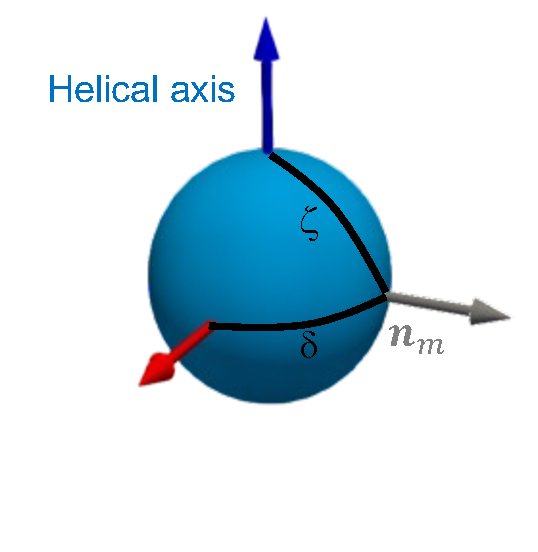
\includegraphics[width = 0.4 \columnwidth]{figures/chapter-3/deldisc}
	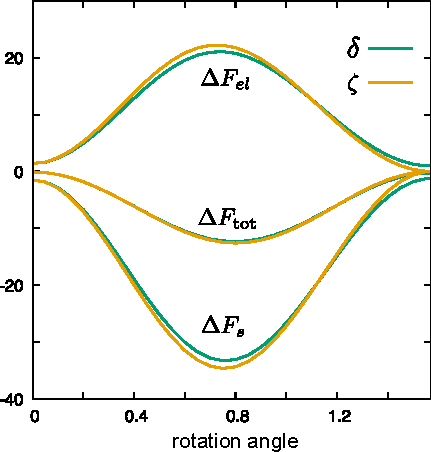
\includegraphics[width = 0.5 \columnwidth]{figures/chapter-3/discelastic}
	\caption[ Distortion free energies (in units $k_{B}T$) around a disc immersed at an angle $\delta$ or $\zeta$ with the local host director]{ Distortion free energies (in units $k_{B}T$) around a disc immersed at an angle $\delta$ or $\zeta$ with the local host director. The distortion free energies remain relatively weak for all $\delta$, but are most pronounced at oblique angles $\delta \sim \pi/4$. Parameters are based on the experimentally relevant situation: $qD =0.4$ and $\ell_{s}/D = 3$ ($W_{0} = 10^{-6} J/m^{2}$). }
	\label{discel}
\end{figure}






\begin{figure}
	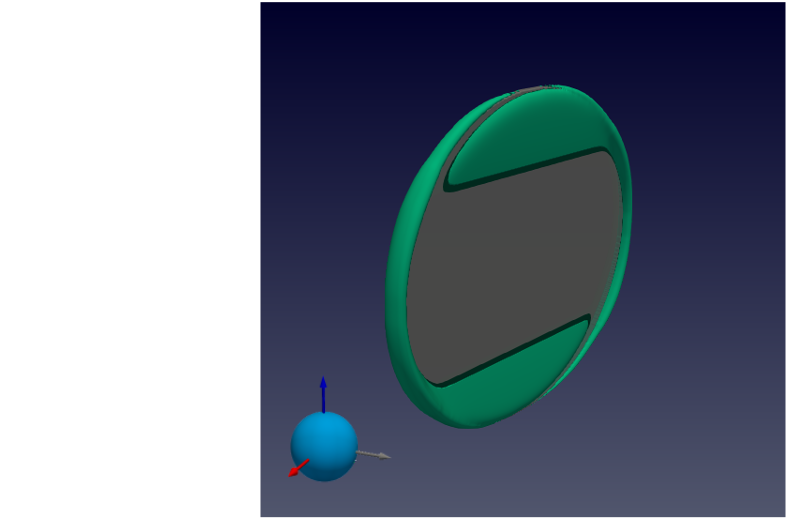
\includegraphics[width =  .5\columnwidth]{figures/chapter-3/chiraldisc}
	\caption[Computer simulation snapshot demonstrating the chiral defect structure (colored in green)]{Computer simulation snapshot demonstrating the chiral defect structure (colored in green) around a disc with hometropic surface anchoring immersed in a molecular cholesteric host LC. Picture courtesy of Jason Wu (University of Colorado, USA). }
	\label{chirdisc}
\end{figure}






We  finish our analysis by considering the case where the disc normal rotates within the $xz$-plane over an angle $\zeta = \tfrac{\pi}{2} - \theta$ away from the molecular director (grey) as indicated in \fig{discel}. In this situation, the tilting will generate additional weak distortions  across the $z$-direction that we denote by the angle $\chi$. The spatially-dependent host director now reads:
\begin{align}
\bn_{s}(\bfr) = & \begin{pmatrix}
\cos \Phi(\bfr)  \cos \chi(\bfr)\\
\sin  \Phi(\bfr) \cos \chi(\bfr) \\
 \sin \chi(\bfr)
 \end{pmatrix}
\label{nseblue}
\end{align}
with $\bfr = ( x,y )$. As before each distortion angles obeys the Laplace equation in the $xy$-plane:
\begin{align}
(\partial_{x}^{2} + \partial_{y}^{2}) \Phi  &= 0 \nonumber \\
(\partial_{x}^{2} + \partial_{y}^{2}) \chi  &= 0
\end{align}
The surface anchoring free energy now takes the following form:
\begin{align}
F_{s} &=  -\frac{W_{0}}{2} \oint d{\mathcal S}  [\bn_{s} \cdot  (  \mathcal{R}_{\zeta} \mathcal{R} (qz) \cdot  \bn_{0}({\mathcal S}))]^{2}
\label{raporotdisc2}
\end{align}
where the matrix $\mathcal{R}_{\zeta}$ describes a rotation of the disc normal within the $xz$-plane:
\beq
\mathcal{R}_{\zeta}=
\begin{pmatrix}
\cos \zeta & 0 & \sin \zeta \\
0 & 1 & 0 \\
-\sin \zeta & 0 &  \cos \zeta \\
\end{pmatrix}
\eeq
Analogous to the previous case, we may derive boundary conditions from linearizing $F_{s}$ for weak distortions $\Phi \ll 1$ and $\chi \ll1$. Plugging in the general solution [\eq{seriesxy}] and defining $b_{n}$ as the distortion modes pertaining to $\Phi(x,y)$ and $d_{n}$ as those for $\chi(x,y)$ we find that both distortion angles are intricately coupled, as expected:
\begin{align}
b_{n} &=  c_{n} \cos \zeta \sin (2 q z) \nonumber \\
d_{n} & = c_{n} \sin (2 \zeta) \cos^{2} (q z)
\end{align}
From these we immediately assert  the most basic scenarios; both distortions vanish for a disc in an achiral host ($q=0$) at zero tilt ($\zeta=0$), whereas at nonzero tilt angle only $\chi(d_{n}) $ is nonzero. For a disc immersed in a chiral host ($q \neq$) at zero tilt ($\zeta =0$) we recover the previous scenario with $\Phi(b_{n})$ given by \eq{bnscenario1} and $\chi(d_{n}) =0$]. Both distortion angles are expected to be nonzero in case the disc normal is tilted away from the local director of the chiral host. The common prefactor reads:
\beq
c_{n} = \frac{ 2\left ( \frac{1-(-1)^{n}}{n \pi}\right )}{1 + 2\ell_{s} n \pi  -\cos( 2 \zeta) - 2 \cos^{2} \zeta \cos (2 q z)}
\eeq
The change in elastic free energy is a simple superposition of amplitudes:
\beq
\Delta F_{el} = \frac{\pi KD}{4}  \int_{-\pi/2}^{\pi/2} d \alpha \cos \alpha \sum_{n} n \left ( b^{2}_{n} + d_{n}^{2} \right )
\eeq
The contribution arising from the host chirality turns out zero for symmetry reasons:
\begin{align}
 \Delta F_{\rm chiral} &=  K q \int d \bfr \partial_{y} \chi (x,y) =0
\end{align}
which is easily inferred from inserting the expansion \eq{seriesxy} and integrating over $y$.
The reduction in surface anchoring free energy caused by the distortions  $\Phi$ is as follows:
\begin{align}
\Delta F_{s, \Phi} = W_{0}D^{2} \cos \zeta  \int_{-\pi/2}^{\pi/2} d \alpha \cos^{2} \alpha \sin (2 qz) \nonumber \\
\times \sum_{n} b_{n} \left ( \frac{1-(-1)^{n}}{n \pi}\right )
\end{align}
supplemented with a similar contribution accounting for the distortions $\chi$:
\begin{align}
\Delta F_{s, \chi} = W_{0}D^{2} \sin( 2 \zeta ) \int_{-\pi/2}^{\pi/2} d \alpha \cos^{2} \alpha  \cos^{2} (qz) \nonumber \\
\times \sum_{n} d_{n} \left ( \frac{1-(-1)^{n}}{n \pi}\right )
\end{align}
Note the surface anchoring is always negative and should outweigh the cost in elastic free energy. The results in \fig{discel} demonstrate that elastic distortions are most developed at oblique orientations, and do not strongly depend on the direction along which the disc is tilted.

\begin{figure}
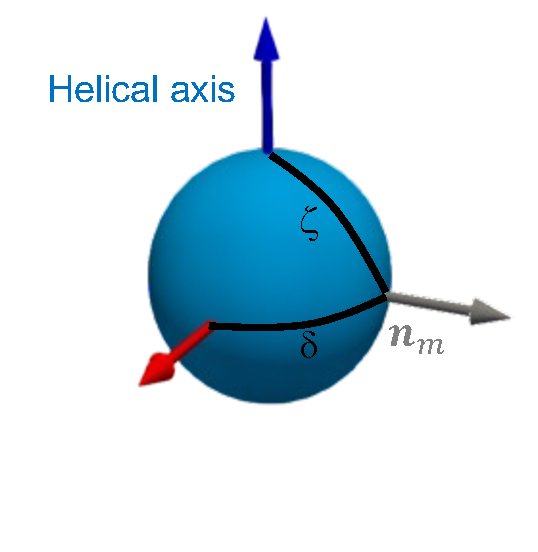
\includegraphics[width = 0.25 \columnwidth]{figures/chapter-3/deldisc}
	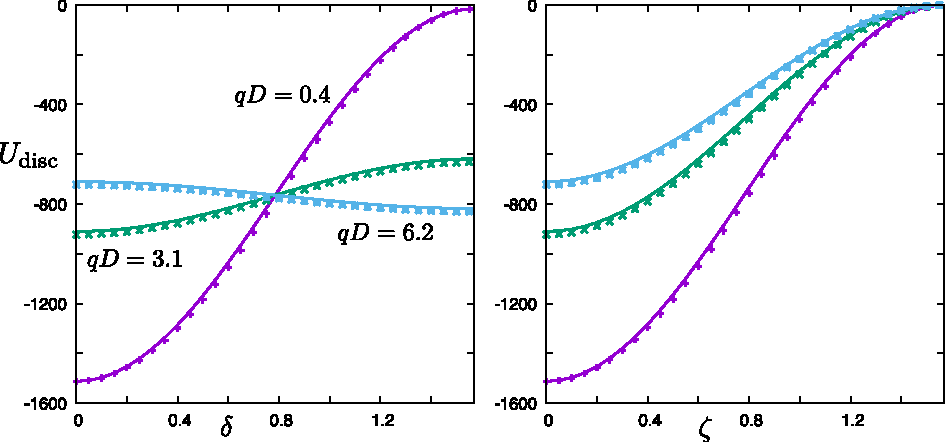
\includegraphics[width = 0.7 \columnwidth]{figures/chapter-3/udisc}
	\caption[Free energy of a colloidal disc with weakly homeotropic surface anchoring immersed in a cholesteric host]{Free energy of a colloidal disc with weakly homeotropic surface anchoring immersed in a cholesteric host with pitch $qD$ as a function of its orientation with respect to the local cholesteric director.  Solid lines correspond to surface anchoring only  [\eq{usp}], while the symbols denote the surface anchoring free energy including weak elastic distortions around the disc.  }
	\label{udisc}
\end{figure}

 If we now reconsider the {\em total} alignment potential for discs accounting for corrections derived above we conclude that the ordering of the discs is hardly affected by the distortions. The free energy changes are typically several tens of $k_{B}T$ which is about two orders of magnitude smaller than the typical Rapini-Papoular surface anchoring free energy $ W_{0} D^{2} $ which is about 1500 $k_{B}T$. Discs experiencing weak surface anchoring with  a cholesteric host with large pitch ($qD <1$)  will therefore simply follow the local molecular director with thermal fluctuations around the optimum angle being strongly suppressed. The considerable penalty incurred  by angular fluctuations away from the local cholesteric director is demonstrated in \fig{udisc} for a number of different host pitches. The elastic distortions around the disc surface lead to a systematic reduction of the free energy, as expected, but their effect on the realigning properties is rather marginal. At short pitches, the disc takes ona preferred angle $\delta = \pi/2$ and aligns along the red arrow, leading to pronounced local biaxial order as highlighted in \fig{disop}. 


 


\section{Conclusions}


We have  demonstrated that immersing uniaxial, non-chiral colloidal rods and disks into a low-molecular-weight cholesteric liquid crystal host leads to emergent biaxial order that we identify by combining experiment with numerical simulation and analytical theory. Unlike the previously studied case of hybrid molecular-colloidal biaxial phases \cite{liu2016,mundoor2021,mundoor2018}, we observe multi-level biaxial symmetry-breaking at ultralow colloidal content where colloid-colloid interactions are negligible. By exploring a variety of colloidal shapes and surface anchoring symmetries we report biaxial order emerging at three distinct levels. First, molecular director distortions develop around each colloid which, although being of marginal extent because of weak surface anchoring conditions, display a distinct two-fold signature imparted by the cholesteric host. Second, the orientational distribution of the colloids around the local cholesteric director is demonstrated to adopt a clear biaxial signature, and the response of the corresponding biaxial order parameter is found to depend non-trivially upon the surface anchoring strength as well as the ratio of the cholesteric pitch and the principal colloidal dimension (rod length or disk diameter). 

A particularly striking manifestation of biaxial symmetry-breaking is encountered for thermotropic cholesterics doped with colloidal rods with homeotropic surface anchoring. Driven by a combination of surface anchoring forces and an energy penalty incurred by twisting a weakly developed surface disclination along the rod main axis, these rods have a strong tendency to align perpendicular to both the helical axis and the local cholesteric director, thus imparting a two-fold $D_{2h}$ orientational symmetry onto the hybrid system at each point along the cholesteric helix.
By means of a simple mean-field theory based on the Rapini-Papoular surface anchoring energy combined with an analytical elasticity theory addressing the corresponding elastic distortions incurred by the presence of the colloids, we have revealed that the multi-level expression of emergent biaxiality in our systems is essentially a single-colloid effect that can be achieved in a wide variety of cholesteric systems doped with non-isotropic colloids. The next chapter will deal with possible scenarios that could arise when the colloid concentration is no longer negligible, and direct correlations between the colloids interfere with the surface anchoring effects discussed in this chapter. 




\clearpage % Disk-polymers

\chapter{Bi-helical order and demixing in hybrid chiral LCs}
\chaptermark{Hybrid LCs: correlation effects}
\label{col_cholesterics}


\begin{abstract}

We extend Onsager's theory to the case of hybrid molecular liquid crystals (LC) composed of colloidal particles immersed in thermotropic host. This framework enables us to explore colloid concentrations that are no longer infinitely small. Correlations between the colloids cause additional entropic and elastic contributions that interfere with surface anchoring effects explored in the previous chapter.  We consider two distinct regimes, namely weak coupling where surface anchoring only marginally impacts the colloid orientations and strong coupling where the typical realignments energy strongly exceeds the thermal energy. We demonstrate at weak coupling that collective colloidal effects driven by steric colloid-colloid interaction may lead to liquid-liquid phase separation between two biaxial fluid phases. In the strong coupling regime, we argue that elastic force may facilitate the formation bi-helical states where the helical organization of the colloidal and molecular components is unequal in pitch and even in handedness. 

\end{abstract}



\section{Introduction}

In the previous chapter we have studied  ordering of colloidal particles in so-called hybrid chiral liquid crystals composed of colloidal particles immersed in a low-molecular-weight cholesteric LC. Inspired by experimental work of we restricted our attention to the regime of low colloidal content where the principal ordering effect stem from single colloid properties related to surface anchoring and elastic distortions formed around the colloid surface. In this regime,  the average interparticle distance remains sufficiently large to guarantee that direct interactions between colloids, mediated by steric collisions or guided by some interference of surface defects, is unimportant. Raising the concentrations of colloids, which has not  been pursued in experiment thus far, offers interesting perspectives to explore the interplay between surface anchoring and alignment driven by colloid-colloid interactions as well as the role of (twist) elastic forces imparted by steric correlations between the colloids. In this chapter we generalize Onsager's theory suitably adapted to treat spatially non-uniform director field such as in a cholesteric, to explore the ordering of colloids at large concentrations where entropic and elastic contributions imparted by the colloids play a role. In doing so we consider two extreme cases, namely weak coupling where colloid realignemt cause by surface anchoring forces is weak, and strong coupling where such realignment is strong compared to the typical thermal fluctuations the colloid experience.  We highlight two main effects (i) surface-anchoring-driven  phase separation between two orthorhombic liquids at weak surface anchoring coupling and (ii) the formation of bi-helical chiral hybrid liquid crystals at large coupling strength.  Since the latter case should occur for both rods and discs alike exploring mixed molecular-colloidal LCs with inherent chirality opens up ways to create chiral fluids composed of discotic mesogens \cite{bisoyi2010discotic,bushby2002discotic}.   



\section{Second-virial density functional }

 With the single-colloid properties fully specified in the previous chapter, we now proceed towards describing the many-particle system by invoking a simple Onsager-type density functional theory \cite{Onsager}. The grand potential $\Omega$ of an assembly of colloids in the presence of an external  potential  reads in general form \cite{allenevans}:
 \begin{align}
 &  \Omega[\rho ]  = \int d \bfr d \bhu  \rho(\bfr, \bhu) \left [k_{B}T \ln {\mathcal V}   \rho(\bfr, \bhu)  +   U_{\rm ext}(\bfr, \bhu) - \mu  \right ] \nonumber \\
 & -\frac{k_{B}T}{2} \int d \bfr d \bhu \int d \bfr^{\prime} d \bhu^{\prime}  \rho(\bfr, \bhu)  \rho(\bfr^{\prime}, \bhu^{\prime}) \Phi(|\bfr - \bfr^{\prime}|, \bhu, \bhu^{\prime} )
 \label{grandpot}
 \end{align}
 with ${\mathcal V}$ denoting an effective thermal volume comprising contributions from rotational momenta and $\mu$ a chemical potential that controls the overall colloid concentration.  The first contribution describes an ideal gas of  non-interacting colloids while the second accounts for colloid-colloid interaction on the second-virial level. Here, the key input is the Mayer function $\Phi$  that, assuming the colloid interactions to be purely hard, renders minus unity if the cores of two colloids overlap and zero if they do not.

 We assume that the colloid positions remain randomly distributed. The orientational probability, however, will be affected by a helical rotation of  the  colloidal director field $\bn(z)$. Since the cholesteric pitch $\lambda \approx 30 \mu m$ is about an order of magnitude larger than the typical colloidal size (a few $\mu m$), the colloidal director is completely enslaved to the rotation of the local cholesteric director and adopts the same pitch length $\lambda$. A $\pi/2$ phase shift between the colloidal director $\bn(z)$ and the cholesteric one $\bn_{s}(z)$ may occur under certain anchoring conditions as we observe in Figs. 1 and 2.  This scenario may no longer hold at larger colloid concentrations and/or shorter cholesteric pitches where the twist elasticity of the colloids becomes considerable, as we will contemplate in a later section. Let us proceed by parameterizing the one-body density in terms of an overall density $\rho = N/V$ and an orientational probability that explicitly depends on the position $z$ along the helix:
 \beq
  \rho(\bfr, \bhu) = \rho f_{q}(\bhu \cdot \bn(z))
 \eeq
 In order to elaborate the grand potential we parameterize the system volume in cylindrical coordinates $d \bfr  = d \bfr_{\perp} dz$ with $0< |r_{\perp}| < \infty$ and $0< z < 2 \pi/q$. Given that the overall rod density is prescribed, the grand potential becomes a Helmholtz free energy $F$. The ideal (translation plus orientation) entropy  free energy per unit volume follow from:
  \begin{align}
 & \frac{ \beta F_{\rm id}}{ V} =  \int d \bhu \int_{0}^{2\pi}  \frac{d(qz)}{2 \pi} f_{q}( \bhu \cdot \bn(z))  \ln [{\mathcal V} \rho  f_{q}( \bhu \cdot \bn(z))]
 \end{align}
Since the orientational distribution does not change along the cholesteric director the ideal free energy density simplifies into the conventional form:
 \begin{align}
  \frac{ \beta F_{\rm id}}{ V} =  \rho \int d \bhu \ln [{\mathcal V} \rho  f_{q}( \bhu \cdot \bn)] f_{q}( \bhu \cdot \bn)
 \end{align}
 with $\bn$ denoting the local director along the helix. Similarly, the external potential in \eq{grandpot} is associated the surface anchoring free energy obtained from the Rapini-Papoular expression \eq{usurf}. It is  defined in the angular coordinates $\bhu(\theta, \delta)$ that co-rotate with the helical director so that:
\beq
\frac{F_{\rm s}}{V} = \rho \int d \bhu   f_{q}(\bhu \cdot \bn)  F_{s}(\bhu)
\eeq
Next, we introduce a linear coordinate transformation $z^{\prime} = z + \Delta z$ and write the excess free energy as follows:
  \begin{align}
  \frac{ \beta F_{\rm ex}}{ V}  = & \frac{\rho^{2}}{2} \int_{0}^{2 \pi}  \frac{d(qz)}{2 \pi}  \int d \bhu \int d \bhu^{\prime}  f_{q}( \bhu \cdot \bn(z)) \nonumber \\
  & \times \int_{-\lambda}^{\lambda} d \Delta z  {\mathcal A}(|\Delta z | , \bhu, \bhu^{\prime} ) f_{q}( \bhu^{\prime} \cdot \bn(z+\Delta z))
 \end{align}
 where  ${\mathcal A}$  is an orientation-dependent excluded {\em area} of rod or disc. The excess free energy is non-local since it depends on volume exclusion between a reference particle at $z$ and test particle  at $z+ \Delta z$ over which the local director will have rotated. It is therefore expedient to apply a transformation $\bhu^{\prime} \rightarrow \mathcal{R} (q\Delta z) \bhu^{\prime}$  which projects the orientation of the test colloid into the director frame of the reference one located at $z$ via the rotation matrix:
 \beq
 \mathcal{R} (q\Delta z)   =
  \begin{bmatrix}
     \cos(q\Delta z)  & \sin(q\Delta z) & 0   \\
   - \sin(q \Delta z) & \cos(q\Delta z) & 0  \\
   0 & 0 &  1  \\
      \end{bmatrix}  \nonumber
      \label{rota}
 \eeq
 The renders the excess free energy local so that it may be simplified into a compact form:
 \begin{align}
  \frac{ \beta F_{\rm ex}}{ V}  = & \frac{\rho^{2}}{2} \int d \bhu \int d \bhu^{\prime}  f_{q}( \bhu \cdot \bn) f_{q}( \bhu^{\prime} \cdot \bn) {\mathcal K}_{q}(\bhu, \bhu^{\prime})
 \end{align}
in terms of and excluded volume that takes into account the helical rotation of the director field:
\beq
 {\mathcal K}_{q}(\bhu, \bhu^{\prime}) =  \int_{-\lambda }^{\lambda} d \Delta z {\mathcal A}(|\Delta z | , \bhu, \mathcal{R}(q\Delta z)  \bhu^{\prime} )
\eeq
This clearly represents a highly convoluted object that we were only able to analyze analytically for thin hard rods, as discussed in the Appendix.
 As alluded to before, in the experimental situation the director twist is weak on the scale of the typical colloid size and it is justified to assume
\beq
 {\mathcal K}_{q}(\bhu, \bhu^{\prime}) \approx {\mathcal K}_{0}(\bhu, \bhu^{\prime}) =  v_{0}| \sin \gamma|
\eeq
which corresponds to the conventional excluded volume between two (infinitely) thin hard rods ($v_{0} = 2 L^{2}D$) or discs ($v_{0} = \tfrac{\pi}{2}D^{3}$), as per Onsager's original theory \cite{Onsager}. This approximation ignores any twist elastic resistance imparted by the colloids and should hold only for low to moderate colloid concentrations and weak director twist ($\lambda \gg L$ or $D$).  The effect of finite twist elasticity will be considered in an upcoming Section.


\begin{figure}
	\includegraphics[width = 0.8\columnwidth]{figures/chapter-4/fcorr3}
	\caption{ Unit-sphere projections of the local orientational probability of rods immersed in a low molecular-weight cholesteric phase at different surface anchoring strengths $\bar{W} = \beta W_{0}LD$, in the presence of a low-correlated colloidal liquid crystal composed by particles of the same kind.  The rod concentration represented here is  $c= \rho L^{2} D = 3$ which corresponds to an isotropic bulk system in the absence of surface anchoring. For all distributions, the rod-length-to-pitch is $qL=1$.}
	\label{fcorr3}
\end{figure}

   \begin{figure}
	\includegraphics[width = 0.8\columnwidth]{figures/chapter-4/fcorrd3}
	\caption{ Unit-sphere projections of the local orientational probability of discs immersed in a low molecular-weight cholesteric phase at different surface anchoring strengths $\bar{W} = \beta W_{0}D^2$, in the presence of a low-correlated colloidal liquid crystal composed by particles of the same kind.  The disc concentration represented here is  $c= \rho D^3 = 3$ which corresponds to an isotropic bulk system in the absence of surface anchoring. For all distributions, the disc-size-to-pitch is $qD=1$.}
	\label{fcorrd3}
\end{figure}
Combining all free energy contributions and formally minimizing the Helmholtz free energy with respect to $f_{q}$ yields a Boltzmann distribution similar to \eq{fsingle}:
   \beq
  f_{q}( \bhu ) = \mathcal{N} \exp \left (- \beta  F_{s} (\bhu) - \rho \int d \bhu^{\prime} f_{q}( \bhu^{\prime} ) {\mathcal K}_{0}(\bhu, \bhu^{\prime})  \right )
  \label{fcollec}
  \eeq
  which reduces to the ideal gas probability \eq{fsingle} for vanishing rod density $\rho = 0$ as it should. The above condition needs to be solved iteratively for a given combination of dimensionless parameters pertaining to the rods (discs), namely the  cholesteric pitch $qL$ ($qD$), surface anchoring strength $\beta W_{0}LD$ ($\beta W_{0}D^{2}$) and colloid concentration $c = \rho L^{2}D$ ($\rho D^{3}$). Possible phase transitions can be probed from the osmotic pressure $\Pi \equiv \partial F/\partial V|_{N,T}$ and chemical potential $\mu \equiv \partial F /\partial N|_{V,T}$ which read:
  \begin{align}
  \beta \Pi  &= \rho + \frac{\rho^{2}}{2} \langle \langle {\mathcal K}_{0}(\bhu, \bhu^{\prime}) \rangle \rangle _{f_{q}} \nonumber \\
  \beta \mu &= \ln [\rho v_{0}] + \langle \ln [f_{q} (\bhu)] + \beta F_{s}(\bhu)\rangle_{f_{q}} + \rho \langle \langle {\mathcal K}_{0}(\bhu, \bhu^{\prime}) \rangle \rangle_{f_{q}}
  \end{align}
  The  brackets are shorthand for an orientational average $ \langle  \cdot  \rangle_{f_{q}} = \int d \bhu   f_{q}(\bhu )(\cdot)$ measured with respect to the local director.


   \section{Orthorhombic liquid-liquid phase separation}

In the absence of surface anchoring realignment ($\bar{W} = 0$) the colloids undergo a conventional isotropic-uniaxial nematic transition. This is the classic Onsager scenario where an isotropic (I) phase  ($c_{I} = 4.19$, $S_{I} =0$) coexists with a (uniaxial) nematic phase  ($c_{N} = 5.34$, $S_{N} =0.792$). For $\bar{W} >0$ the $O(3)$ symmetry of the isotropic phase and the uniaxial $D_{\infty h}$ symmetry of the nematic will both be broken in favour of a biaxial, orthorhombic symmetry ($D_{2h}$), and a coexistence between two orthorhombic phases with different overall colloidal concentrations is expected. Resolving the coexistence conditions by imposing equality of chemical potential $\mu$ and pressure $\Pi$ in both phases we may explore phase diagrams in the surface anchoring amplitude - colloid concentration ($\bar{W} - c$) plane. The results are shown in \fig{phdiag} and demonstrate that a phase coexistence between two orthorhombic nematic phases is indeed possible in the weak coupling regime ($\bar{W} <1$). A critical point beyond which no phase transition is possible is located at a surface anchoring energy equivalent to a few times the thermal energy.

   \begin{figure}
	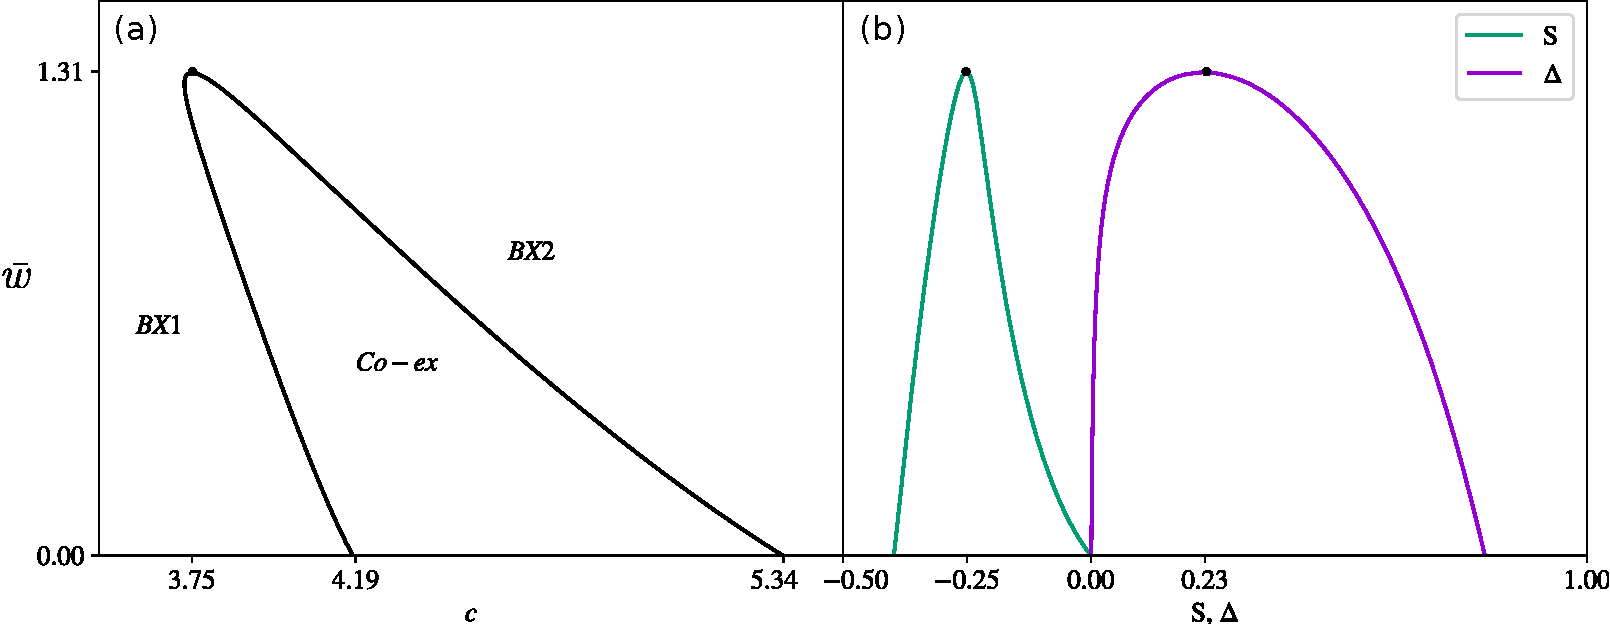
\includegraphics[width = .9\columnwidth]{figures/chapter-4/diagrams_q0.335_horizontal}
	\caption{(a) $\bar{W} - c $ phase diagram for rods with homeotropic or tangential surface anchoring, $qL = 0.335$. (b) Corresponding uniaxial (solid line) and biaxial (dashed line) nematic order. A qualitatively equivalent scenario can be found for discs with planar surface anchoring.}
	\label{phdiag}
\end{figure}


   \begin{figure}
	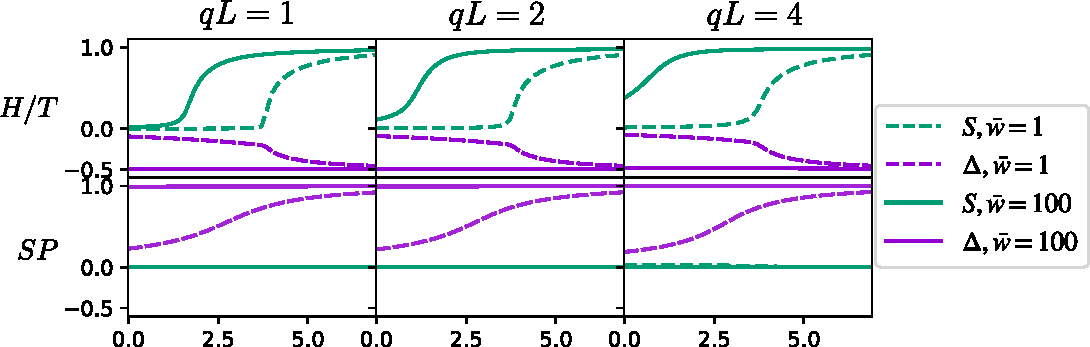
\includegraphics[width = \columnwidth]{figures/chapter-4/ordervsc_rods}
	\caption{ Uniaxial $S$ and biaxial $\Delta$ order parameters measured along the cholesteric nematic direction $\bn_{m}$ as a function of the concentration $c = \rho L^{2}D$ ($\rho D^{3}$) for rods at low (dashed lines) and high (solid lines) surface anchoring strength ($\bar{W} = \beta W_{0}LD = 1$ and $\bar{W} = \beta W_{0}LD = 100$ respectively) and three different values of $qL$.}
	\label{w1o}
\end{figure}

   \begin{figure}
	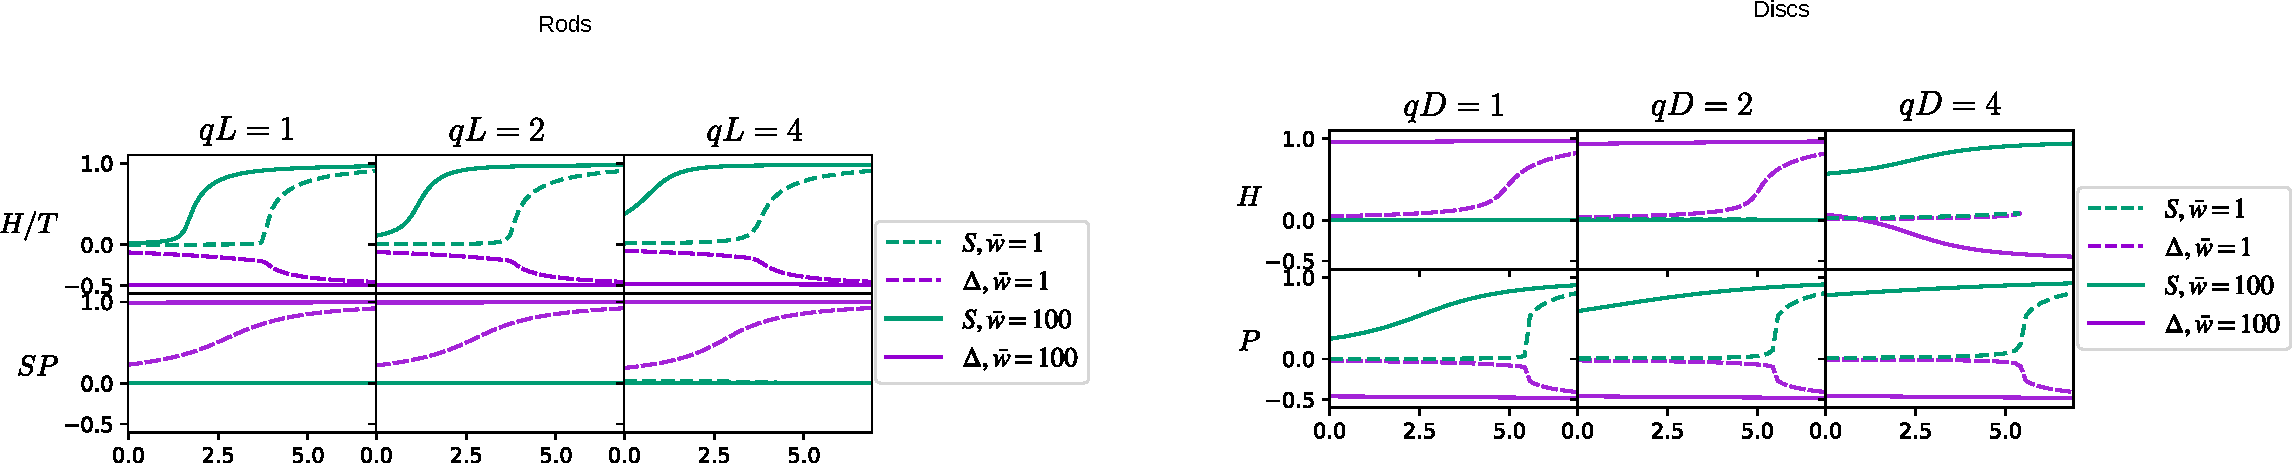
\includegraphics[width = \columnwidth]{figures/chapter-4/ordervsc_discs}
	\caption{ Uniaxial $S$ and biaxial $\Delta$ order parameters measured along the cholesteric nematic direction $\bn_{m}$ as a function of the concentration $c = \rho L^{2}D$ ($\rho D^{3}$) for discs at experimentally typical surface anchoring strength ($\bar{W} = \beta W_{0}D^2 = 1$ and $\bar{W} = \beta W_{0}D^2 = 100$ respectively) and three different values of $qL$.  The concentration domain used in the discotic homeotropic case is more restricted due to  numerical difficulties.}
	\label{w100o}
\end{figure}




\section{Effect of colloid-induced elasticity}

At certain conditions such as strong surface-anchoring coupling and large colloid concentration $\rho$ and short cholesteric pitches the twist elastic resistance generated by the anisotropic colloid-colloid repulsions will prevent the colloidal director from keeping pace with the rotation of the cholesteric director. This  may give rise to hybrid systems in which the colloidal director locally deviates from the the cholesteric helix. Let us attempt to explore this scenario in more detail starting from the cholesteric director field \eq{ns} that we keep fixed in the laboratory frame. In doing so, we rely on three further basic assumptions; (i) the colloids remain uniformly distributed throughout the system and do not affect the cholesteric helix whose  pitch $q$ remains unaffected, (ii)  the colloids are perfectly aligned and exhibit negligible thermal fluctuations around their main orientation, and (iii) the colloidal director remains perpendicular to the helical axis $\bz$ but we allow the degree of local twist to be non-uniform along the $z$-direction. We then parameterize the colloidal director as follows:
\beq
\bn(z) = \bx \cos \phi(z)   + \by \sin \phi(z)
\label{npara}
\eeq
 in terms of a local twist angle $\phi(z)$. Since the system is apolar, the director $\bn$ is equivalent to $-\bn$ so that $\phi(z)$ is equivalent to $\phi(z)  + \pi$.  For the cases discussed thus far, the colloidal director is simply co-helical with the cholesteric so that $\phi(z) =qz$ (mod $\pi )$.

 \subsection{Rods}

 Let us focus first on the case of rods. The fraction of rods aligned along the helical axis $\bz$ (as observed in \fig{fcorr3}) may be disregarded as they contribute very little to the twist elastic resistance imparted by the colloids. Since we assume that the rods are perfectly aligned along the above director we write the rod contour $\bfr_{{\mathcal S}}(t) = \bfr_{0} +  \frac{L}{2}t\bn(z)$ and applying this in the Rapini-Papoular expression \eq{usurf} along with the above parameterization we find:
\beq
F_{s}[\phi(z)]  = - \frac{1}{8} W_{0} LD \begin{cases}
       2 \pi \sin^{2}[\phi(z) -qz ] &  \textrm{H/T} \\
         4 \pi \cos^{2}[ \phi(z) - qz ]  &  \textrm{SP}
   \end{cases}
      \label{plahoms}
\eeq

In the absence of twist elastic effects the surface anchoring energy is indeed minimized along a uniform twist profile $\phi(z) = qz + \phi_{0} $ with phase shifts $\phi_{0} = \pi/2$ (H/T) and $\phi_{0} = 0$ (SP) as evident from the result in \fig{fcorr3} and \fig{fcorrd3}.


The (continuum) free energy per unit area reflects a competition between the surface anchoring energy, and a restoring (twist) elastic energy:
\begin{align}
\frac{F}{A} &= \int d z \left \{ \rho F_{s}[\phi(z)]  + \frac{K_{2}}{2} (\bn(z) \cdot \partial \times \bn(z) )^{2} \right \}
\end{align}
with $K_{2}$ the twist elastic modulus of a colloidal nematic system.
Removing the trivial phase angle by rescaling $\phi(z) \rightarrow \phi(z) - \phi_{0}$ and some further basic manipulation we obtain a universal expression for both anchoring scenarios:
\beq
\frac{F}{A} = \int d z \left \{ -\sigma \cos^{2}[\phi(z)-qz] + \frac{K_{2}}{2} (\partial \phi(z)  )^{2} \right \}
\label{freedens}
\eeq
in terms of surface anchoring energy density $\sigma_{\ds \rm HT} = \tfrac{\pi}{4} \rho W_{0}LD$ and $\sigma_{\ds \rm SP} = 2 \sigma_{\ds \rm HT}$ for the SP case. The corresponding Euler-Lagrange equations reads:
\begin{align}
 K_{2}\phi^{\prime \prime}(z) - \sigma \sin[2 ( \phi(z)- qz)]&=0
 \label{nlde}
 \end{align}
subject to the boundary conditions $\phi(0) = 0$ and $\phi^{\prime}(0) = 0$, i.e., the colloids are kept non-chiral. The effect of chirality will be considered in a subsequent paragraph.
It is convenient to introduce a non-linear twist angle $\varepsilon(z) = \phi(z) - qz$ which measures the local deviation of the colloidal director from the cholesteric one. Both anchoring situations can then be described by a sine-Gordon equation:
\beq
 \xi^{2} \varepsilon^{\prime \prime}(z) = \sin[2\varepsilon(z) ]
\label{diffeps}
\eeq
It features the following length scale:
\beq
\xi = \sqrt{\frac{K_{2}}{\sigma}}
\eeq
The  solution under is non-analytical and can be written in terms of (inverse) elliptic functions:
\beq
\phi(z) = qz -\textrm{am} (qz, -2/(q\xi)^{2})
\label{jaf}
\eeq
with $\textrm{am}(x,k)$ denoting the Jacobi amplitude function which has the known limit $ \textrm{am}(x,0) = x$. From this we conclude that an untwisted director profile $\phi(z) = 0$ is found at infinite elasticity $q\xi \rightarrow \infty$, as should be the case. At large but finite $q\xi$ the colloidal helix unwinds with respect to the cholesteric and adopts an (average) pitch $q_{c} <q$, leading to a bi-helical hybrid system. This scenario is depicted in \fig{unwind}. Interestingly, at $q\xi >1$ the colloidal helix not only unwinds, it also adopts a handedness that is opposite that of the cholesteric helix.  Associated with the unwound colloidal director are periodic ``breathing" fluctuations whose amplitude and period are shown in \fig{fluc}.  These fluctuation are easily fitted to a periodic profile so that (for $q \xi >1$):
\beq
\phi(z) -q_{c}z \approx   \delta \phi e^{  i q_{b} z }
\label{nlinrip}
\eeq
in terms of an amplitude $\delta \phi$ and periodicity $q_{b}$. The amplitude slowly decays as $q \xi \rightarrow \infty $ while the breathing periodicity attains a constant value $q_{b}/q \rightarrow 2$.


   \begin{figure*}
	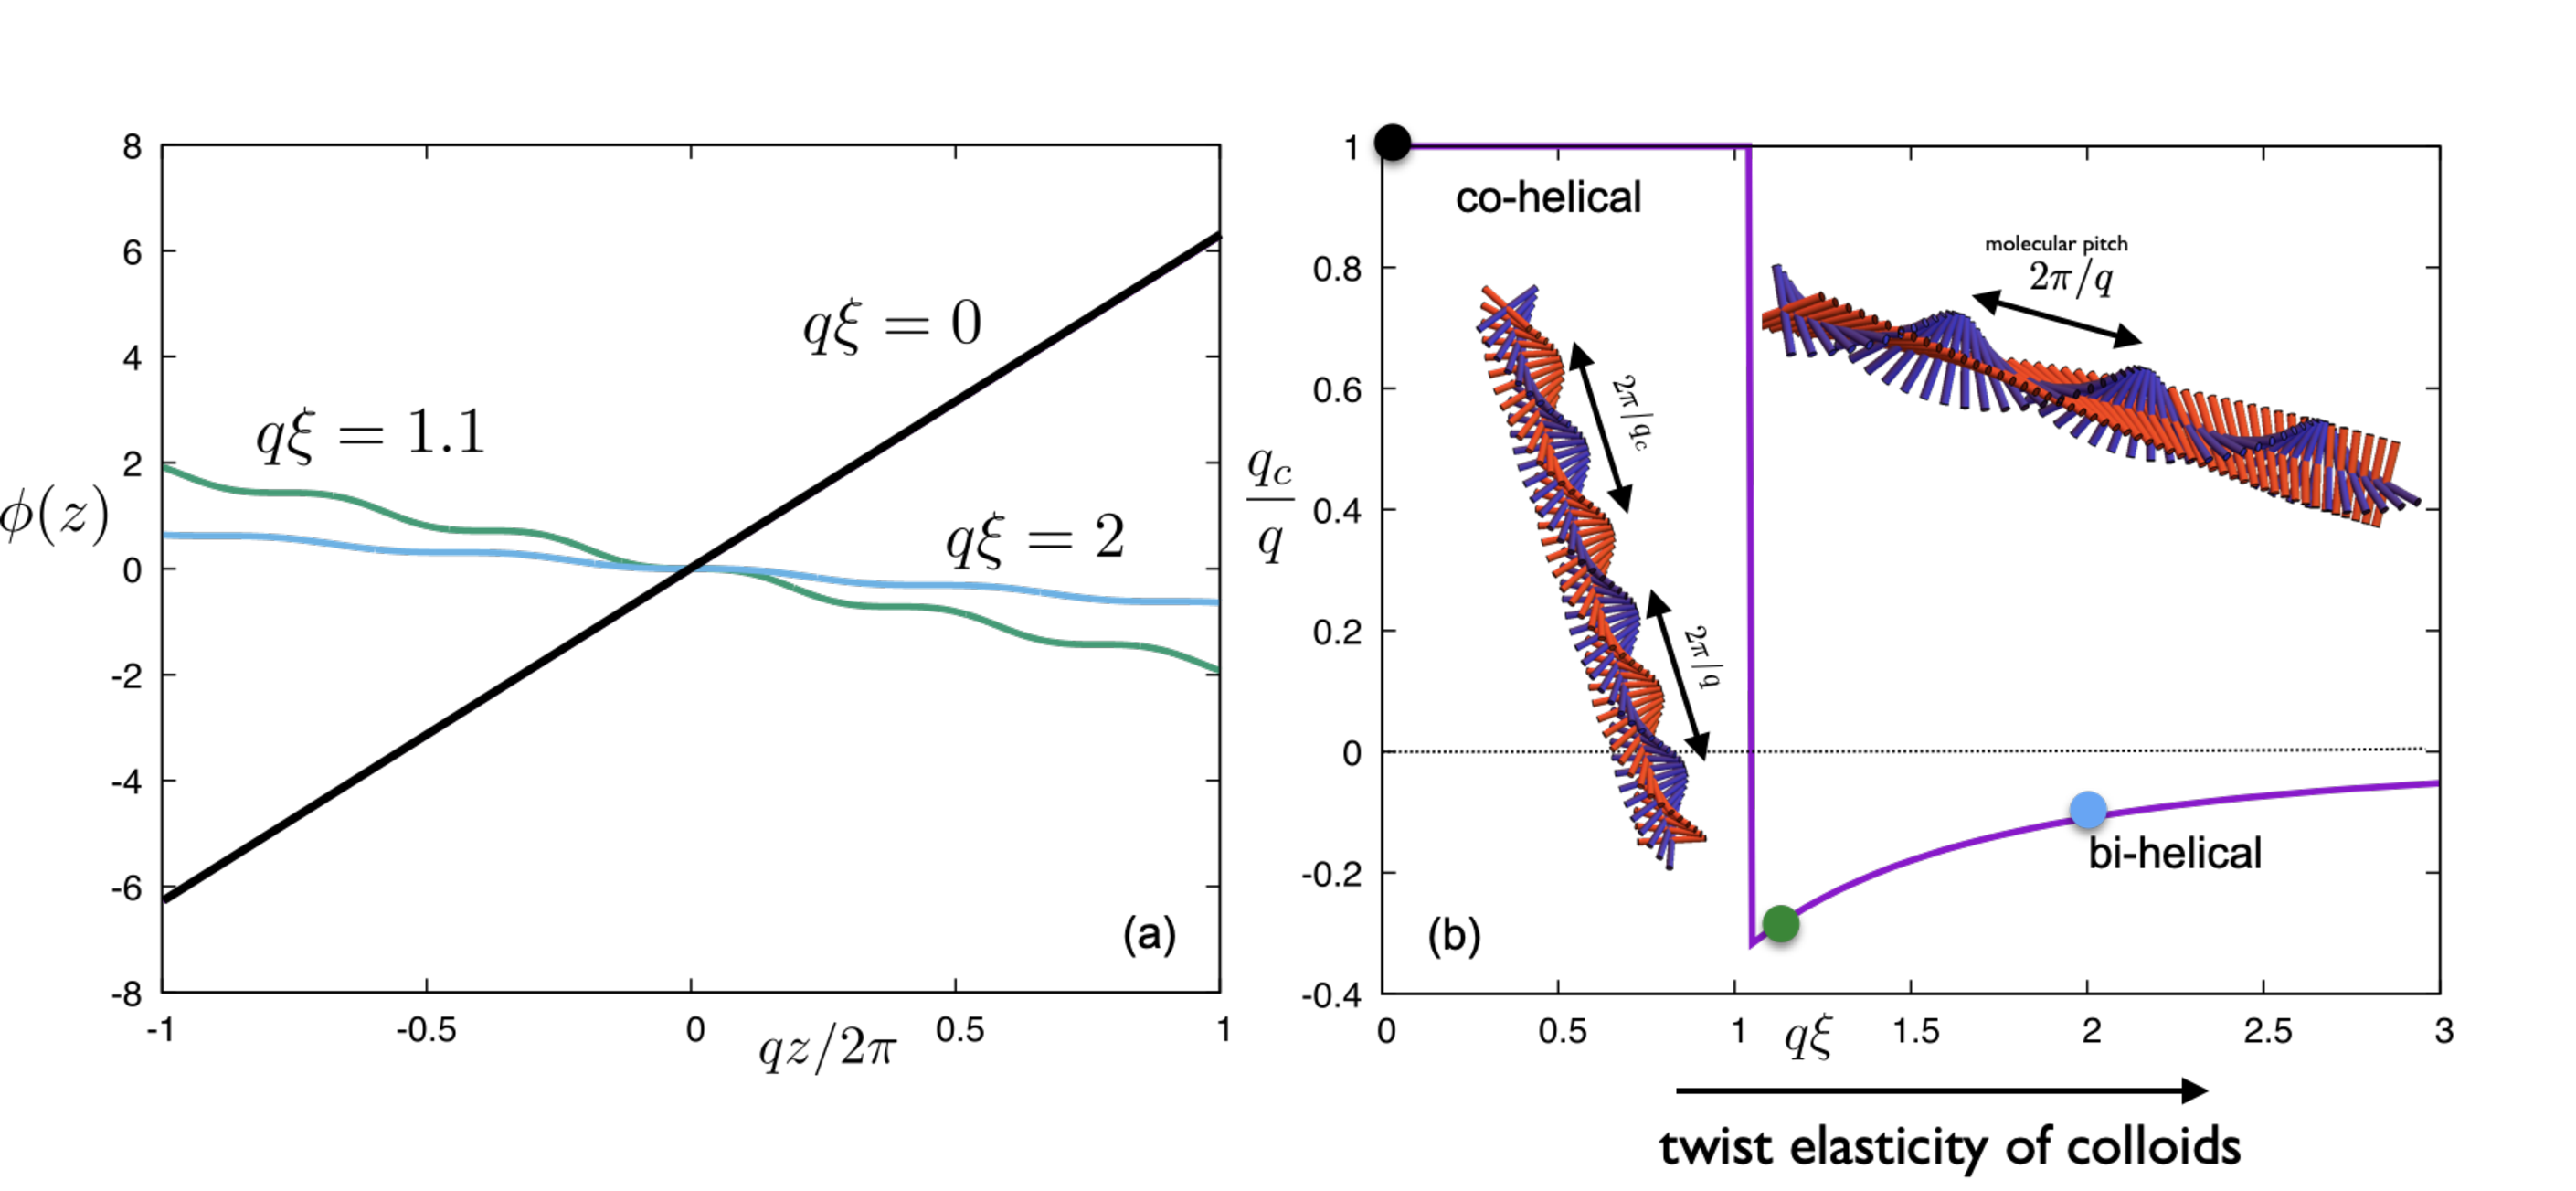
\includegraphics[width =  \columnwidth]{figures/chapter-4/bihelical}
	\caption{ (a) Twist angle $\phi(z)$ of the colloidal director along the helical direction for different strengths of the twist elasticity of the colloids. At weak twist elasticity  ($q \xi <1$) the colloidal director remains co-helical with the cholesteric helix.  At $q \xi >1$ unwinding of the colloidal helix occurs with  ``breathing" instabilities.   (b) Evolution of the pitch $q_{c}$ of the colloidal helix with respect to the cholesteric pitch $q$. Note that in the bi-helical regime the cholesteric and colloidal helices have opposite handedness. The colloidal helix is shown in red, the molecular one in blue.   Colored dots indicate the  state-point corresponding to the breathing profiles in (a). }
	\label{unwind}
\end{figure*}


 \begin{figure}
	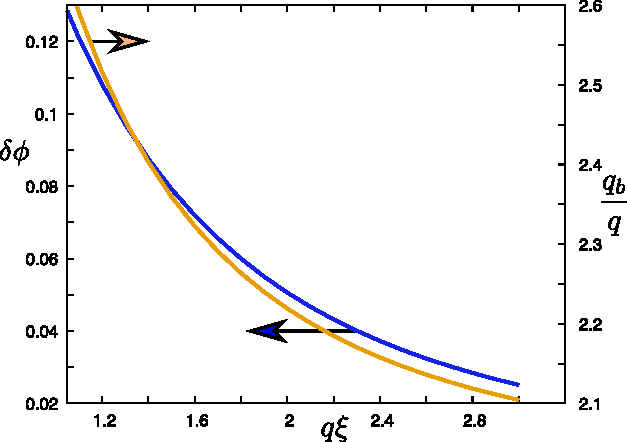
\includegraphics[width = .6\columnwidth]{figures/chapter-4/fluctuations}
	\caption{ Amplitude $\delta \phi$ and periodicity $q_{b}$ of the ``breathing" instabilities encountered in the bi-helical state in \fig{unwind}b as a function of the twist elastic strength $q \xi$. }
	\label{fluc}
\end{figure}

Another common solution that is associated with the sine-Gordon equation is the soliton. Taking the boundary conditions $\varepsilon^{\prime}(\pm \infty) = 0$ and $\varepsilon(\infty) - \varepsilon(-\infty)  = \pi$. The solution for the single soliton can be obtained in analytical form  \cite{kamien2001order}:
\beq
\phi(z) =  qz \pm \frac{\pi}{2} \pm 2 \arctan \left [ \tanh \left ( \frac{z - z_{0}}{R_{s}} \right ) \right ]
\eeq
where $ R_{s} = 2^{1/2} \xi$ defines the soliton width and $z_{0}$ the arbitrary position of its centre along the cholesteric helix. The $-$ solution refers to an anti-soliton. In achiral liquid crystals such as our colloidal subsystem, the (anti-)solitons are unstable with respect to the uniform background (i.e. the co-helical state). The dimensionless free energy difference between the soliton and the co-helical state is  $\tfrac{\Delta Fq}{ A \sigma} = q \xi (2^{3/2} + \pi q\xi)$. However, once they are formed the solitons are metastable and cannot simply relax to the co-helical state without locally destroying nematic order.

From the scaling expression \eq{k2odijk} for the twist elastic constant of rods proposed in the Appendix we find that the soliton width $\sim \xi$ is independent of rod concentration. However, the solitons would be unrealistically small as $\xi $ turns out to be of the same scale as the width of the individual rods, namely  $\xi \sim 70 nm$ for long rods ($L \sim 3 \mu m$ and $D \sim 30 nm$ and $W_{0} = 10^{-5} J/m^{2}$).


\subsection{Effect of rod chirality}

It is well known that conventional (non-hybrid) chiral liquid crystal subject to a uniform electromagnetic field perpendicular to the helical axis may form stable solitons provided that the nematogens are sufficiently chiral \cite{lam2012solitons,ackerman2014two,wu2022hopfions}.  In fact, our rods must have some intrinsic chirality in view of the decoration of helical disclinations imparted by the cholesteric environment, as demonstrated in the previous chapter. The effect of chirality is easily accounted for by an additional free energy \cite{gennes-prost}:
\begin{align}
\frac{F_{\rm chiral}}{A} &= K_{t} \int d z  (\bn(z) \cdot \partial \times \bn(z) )=  K_{t} \int d z (\partial \phi(z) )
\end{align}
with $K_{t}$ denoting the strength of the chiral interactions between the rods. It is customary to identify $K_{t} =q_{r} K_{2}$ where $q_{r}$ would be the pitch of a chiral nematic formed by the rods {\em alone}. In general, $q_{r}$ differs from the pitch $q$ of the cholesteric helix $q$ although a subtle coupling between the two is expected. We stress that $q_{r}$  is a purely hypothetical variable since the rods would not be chiral in the absence of surface anchoring effects imparted by the cholesteric solvent.
Since the chiral contribution is linear in the gradient of $\phi$, the Euler-Lagrange equation \eq{nlde} associated with the total free energy remains unchanged. The boundary conditions now read $\phi(0) = 0$ and $\phi^{\prime}(0) = q_{r}$. If we assume the handedness of the rods to be the same as that of the cholesteric environment, then the main effect of colloid chirality is that the co- to bi-helical transition shifts towards larger $q \xi$. This is a natural consequence of the fact that chirality favors the twisted co-helical state over the (partially) untwisted bi-helical one. Of course, the reverse effect occurs if the rods adopt a handedness that is opposite to that of the cholesteric state ($q_{r} <0$). Then, the transition to the bi-helical state in \fig{unwind}b systematically shifts to smaller $q\xi$ upon increasing the chiral strength $|q_{r}|$.


The free energy between the soliton and the  co-helical state now reads $ \tfrac{\Delta Fq}{ A \sigma} = q \xi [ 2^{3/2}+  \pi q \xi (1-\tfrac{q_{r}}{q})]$. This means that solitons may eventually become stable within the co-helical regime if $\tfrac{q_{r}}{q} > 1 + \tfrac{2^{3/2}}{\pi q \xi}$ which implies that the rods must be very strongly chiral indeed. However, the soliton width is not affected by chirality and remains of the order of the colloid thickness which means that the solitons remain a purely hypothetical scenario, at least within our simple coarse-grained model.

\subsection{Discs}

The case of discs proceeds in an analogous way.  If we assume the same set of basic approximations to hold for the colloidal discs as well, we may start with computing the surface anchoring free energy which takes a simple form  (ignoring irrelevant constants):
\beq
F_{s}[\phi(z)]  =   \begin{cases}
       -\sigma_{\rm \ds H} \cos^{2}[\phi(z) -qz ] &  \textrm{H} \\
        -\sigma_{\rm \ds P} \sin^{2}[ \phi(z) - qz ]  &  \textrm{P}
   \end{cases}
      \label{plahomsdisc}
\eeq
with $\sigma_{\rm \ds H} = \frac{\pi}{4}\rho W_{0}D^{2}\tfrac{J_{1}(qD)}{qD}$ and $\sigma_{\rm \ds P}= \tfrac{1}{2} \sigma_{\rm \ds H}$ describing the two basic anchoring symmetries we consider. Comparing with \fig{fd} we immediately identify the optimal profile $\phi(z) = qz + \phi_{0}$ with $\phi = 0$ (H) and $\phi_{0} = \tfrac{\pi}{2}$ (P) at least for weak to moderate cholesteric pitch $qD < 2$.   Clearly, since the surface anchoring energy has the same basic form  as those previously discussed in \eq{plahoms} for  rods, the director profiles are identical too, provided the  lengthscale $\xi =\sqrt{K_{2}/|\sigma|}$ is taken to be the one appropriate for discs. Using the scaling expression from the Appendix, we find:
\beq
\xi \sim 0.87 c  \sqrt{  \frac{|q|D}{J_{1}(|q|D)}} \sqrt{\frac{k_{B}T}{W_{0}}}
\eeq
which yields about $\xi \approx 80 nm $ for $D = 2 \mu m$ sized discs studied experimentally at a concentration $c = \rho D^{3} =3$, $W_{0} = 10^{-5} J/m^{2}$ and a cholesteric pitch length of $30 \mu m$ corresponding to $qD \approx 0.6$.

For certain values of $qD$ the surface anchoring amplitude $\sigma $may become negative ($\sigma< 0$). In those cases, the phase angles associated with the two anchoring scenarios are simply swapped so that  $\phi = \tfrac{\pi}{2}$ (P) and $\phi_{0} = 0$ (P). By rescaling $\phi(z) \rightarrow \phi(z) - \phi_{0}$ we obtain the  same Euler-Lagrange equation \eq{nlde} with $\sigma \rightarrow | \sigma |$.


\section{Conclusions and outlook}

In this chapter we have theoretically addressed the implications of finite colloid concentration in self-organization of hybrid colloidal-molecular liquid crystals. While at low colloid content the orientation of each colloid is mainly driven my single-particle effect related to surface anchoring and possible surface defects, the phenomenology becomes richer and exciting when colloid-colloid interactions are taken into account. We argue that steric combined with weakly aligning surface anchioring forces may drive liquid-liquid phase separation between two orthorhombic fluid, each with a different colloid concentration and orientational order parameters. In the strong coupling regime, when surface-anchoring-mediated  particle realignement is strong, the colloids impart non-negligible twist elasticity that may stabilize a variety of different bi-helical hybrid LCs in which both molecular and colloidal self-organize along distinctly different helical mesostructures. We also predict the typical colloidal concentration needed to stabilize these structures in experiment. 

At elevated colloid concentration additional interactions could becomes more prominent, for instance those imparted by surface defects and long-range electrostatic forces owing to surface charges residing on the colloids, which will have an impact on the elastic properties generated by the colloids. In fact, one could naively argue  that these could give rise to a significant stiffening of the elastic moduli of the colloidal subcomponent which could lead to a stabilization of bi-helical structures at much lower colloid concentrations than anticipated here.   Clearly, any further quantitative prediction requires a considerable refinement of our analysis beyond the simple steric model considered here.  






%A general solution of \eq{nldereno} under the boundary condition $\varepsilon(0)=0$ can be expressed in terms of the Jacobi amplitude (am) function:
%\beq
%\varepsilon(z) = \textrm{am} \left (qz c_{1}, \frac{2}{- c_{1}^{2} (q\xi)^{2}} \right )
%\eeq
%with $c_{1} > 0$ some unknown constant that needs to be determined from the second boundary condition.







%yields the basic solution $\varepsilon(z) = \varepsilon_{-} \exp(-2^{1/2} z/\xi)+ \varepsilon_{+} \exp(2^{1/2} z/\xi)$. Imposing the boundary condition  $\varepsilon(0) =0$ we find:
%\beq
%\varepsilon(z) = 2\varepsilon_{0} \sinh ( 2^{1/2} z/\xi )
%\eeq
%Since the hyperbolic sine diverges for large $|z|$ the only way to render the solution consistent with $|| \varepsilon ||$ is by setting $\varepsilon_{0} =0$ which means there are no solutions up to linear order in $\varepsilon$.

%Reduction of order leads to
%\beq
%( \varepsilon^{\prime} (z) )^{2} + (q\xi)^{-2} \cos [2 \varepsilon(z)] = C_{1}
%\eeq

\begin{subappendices}
\section{Twist elastic resistance of thin hard needles and discs}

For   hard rods  a tractable analytical expression for the $z-$resolved excluded area is available in the needle limit $L/D \rightarrow \infty$ \cite{poniewierski1988nematic,shundyak2001isotropic}:
\begin{align}
 & {\mathcal A}(|  \Delta z | , \bhu, \bhu^{\prime} ) = -\int d  \Delta \bfr_{\perp} \Phi(|\Delta \bfr |, \bhu, \bhu^{\prime} ) \nonumber \\
 & = 2 L^{2} D |\sin \gamma | \begin{cases}
 0 & |\Delta z| > A+ B \\
 \frac{A + B - |\Delta  z |)}{4 AB } & A - B \leq |\Delta z| \leq A+ B  \\
 \frac{1}{2A} & |\Delta z| < A - B
 \end{cases}
 \label{aexcl}
\end{align}
with $A= \frac{L}{2} | \text{max} ( u_z , u^{\prime}_{z}  ) |$ and $B= \frac{L}{2} | \text{min} (u_{z} , u^{\prime}_{z} ) |$.  We can make headway by realizing that  a rotation of the reference director  only affects the azimuthal angle $\varphi$. More specifically we  have
 ${\mathcal R}(q \Delta z) | \sin \gamma | = \sqrt{1 - (\cos \theta \cos \theta^{\prime}  - \sin \theta \sin \theta^{\prime} \cos (\Delta \varphi - q\Delta z) )^{2}} $
with $\Delta \varphi = \varphi - \varphi^{\prime}$.  Performing the integration over $\Delta z$ we can cast the kernel as a Taylor series in terms of even powers of the colloidal pitch $qL$:
\beq
{\mathcal K}_{q} (\bhu, \bhu^{\prime}) = 2 L^{2} D \sum_{n=0}^{\infty} \frac{(qL)^{2n}}{2n!} a_{2n} (\bhu, \bhu^{\prime})
\eeq
 Note that odd powers in $q$ must vanish since the rods are considered to be achiral. We note that  the immersed rods induce weak distortions of the solvent director which are known to adopt a helical signature that could render the rod-rod interaction chiral.  The angle-dependent factor reads in explicit form:
\begin{align}
a_{2n} (\bhu, \bhu^{\prime}) &=  \frac{(\frac{1}{2}u_{z}+\frac{1}{2}u^{\prime}_{z})^{2n +2} - ( \frac{1}{2}u_{z} - \frac{1}{2}u_{z}^{\prime})^{2n+2}}{ u_{z} u_{z}^{\prime} (2n+1)(n+1)} \nonumber \\
& \times \frac{\partial ^{(2n)} | \sin \gamma |_{q=0}}{\partial \Delta \varphi ^{(2n)}}
\end{align}
and it is easily verified that $a_{0} = | \sin \gamma |$ as required. It is insightful to express the  excess free energy per unit volume in the following way:
\beq
\frac{F_{ex}}{V} = k_{B}T \frac{\rho^{2}}{2} \langle \langle {\mathcal K}_{0}(\bhua, \bhub) \rangle \rangle_{f_{q}} +  \sum_{n=1}^{\infty} \frac{q^{2n}}{2n!} K_{2}^{(2n)}
\label{felast}
\eeq
 The quantities $K_{2}^{(2n)}$ could be interpreted as {\em generalized} twist elastic constants defined as:
\beq
K_{2}^{(2n)} = k_{B}T \rho^{2} L^{2n+2}D \langle \langle a_{2n}(\bhua, \bhub) \rangle \rangle_{f_{q}}
\eeq
for most conventional cholesteric phases the director twist is weak on the scale of the rod ($qL <1$) and the expansion may be truncated after the second term. Furthermore, the  orientation distribution is   unaffected by any director twist so that $f_{q}$ can be approximated by the orientation distribution $f_{0}$ of a non-chiral uniaxial nematic phase. The  quantity $K_{2}^{(2)}$ is then identified as the conventional twist elastic constant for which the microscopic definition reads:
\beq
K_{2}  =K_{2}^{(2)}=  k_{B}T \rho^{2} L^{4}D \langle \langle a_{2}(\bhu, \bhu^{\prime}) \rangle \rangle_{f_{0}}
\eeq
For conventional uniaxial nematic order scaling results exist that relate  $K_{2}$ to the total  rod concentration. Using Gaussian theory Odijk \cite{odijkelastic} found that for asymptotically strong nematic alignment:
\begin{align}
\beta K_{2}D \sim \frac{7}{96} c
\label{k2odijk}
\end{align}
For infinitely thin hard discs a much steeper increase with colloid concentration was found \cite{wensink2018}:
\beq
\beta K_{2}D  \sim 0.606 c^{3}
\eeq
which suggests that lyotropic discotic nematic phases are far more difficult to twist than their rod-based counterparts at equivalent particle concentration (note that $c \gg1$ for most stable nematics).

\end{subappendices}


\clearpage % Cholesterics: single colloid

\chapter{ Twisted membranes versus ribbons in colloidal rod-polymer mixtures}
\chaptermark{Droplet morphology}
\label{twistedrods}



\begin{abstract}

At the mesoscopic level, rigid rodlike colloids with chiral features such as {\rm fd} virus rods mixed with non-adsorbing polymer form a variety of different liquid crystalline droplets with varying shape and internal twisted structure. Inspired by recent experiment work on the droplet morphology of these rod-polymer mixtures, we use extensive Monte Carlo simulations supplemented with theory to explore two prominent droplet shapes, namely the twisted membrane and the ribbon. In experiment, the elongated ribbon structure is found to dominate at elevated chiral strength. In our simulations, however, we demonstrate that upon increasing chirality the membranes tend to transition into multi-domain structures consisting of multiple twisted near-circular units separated by $\pi$-walls, while the transition into twisted ribbons is impeded by the strong surface tension experienced by the droplet. We supplement our simulations with simple microscopic theoretical descriptions for both droplet morphologies which enable us to predict the evolution of the twist angle across the membranes. For the ribbons, our simple theory provides generic predictions for the typical ribbon width, internal twist and edge tilt angle that are in broad agreement with experimental observations of twisted ribbons composed of  {\em fd}
virus rods mixed with dextran. 

\end{abstract}



\section{Introduction}




Rodlike colloidal particles are capable of assembling into a variety of liquid crystalline mesostructures whose bulk properties depend primarily on the topology of the director field indicating the average direction of rod alignment \cite{dogic-fraden_fil,Ikkala2407}.
In general,  site-specific attractive forces between non-spherical nanoparticles may affect the self-assembly properties  and lead to a wealth of different superstructures \cite{Wang358} such as twisted ribbons of semi-conducting rods \cite{Srivastava1355} or platelets \cite{Janae1701483}.
Mixing rodlike colloids with non-adsorbing polymers or other small depletant particles induces a short-ranged attractive  (`sticky') effective potential between the rods that can be exploited to control the self-assemby morphology \cite{Baranov2010,Sharma2014}. 
 


 The size and concentration of the added polymer can be exploited to  tune the morphology and internal structure of the droplets. Tactoids with nematic-type order have been observed experimentally in mixtures of rods and big depletants (typically bigger than the diameter of the colloidal rods), as well as smectic-like single layer droplets, named colloidal membranes, when significantly increasing polymer concentration. The morphology of these membranes is further controlled by strong electrostatic and chiral twist interactions between the individual rods. Though these interactions are not well understood yet, it has been empirically observed that, in close contact with one another, {\em fd} rods tend to twist preferentially clockwise, instead of arrange following a global nematic direction. When both depletion effect and chirality are strong, twisted colloidal membranes tend to destabilize to give way to twisted ribbons. The additional effect of intrinsic particle chirality
strongly impinges  onto the self-assembled mesostructure and drives a vast range of different twisted or chiral structures ranging from smectic membranes to chiral ribbons  \cite{Gibaud2012} and hexagonal nanocrystals displaying screw-dislocations \cite{grelet1}. These twisted structures have been observed experimentally, but reproducing the various mesophases with distincltly different twisted morphologies in computer simulation has been elusive so far.  Modelling efforts have focussed almost exclusively on twisted membranes \cite{kang_sm2016,wensink2018elastic,kuhnhold2022colloidal} or conventional LC tactoids exhibiting full three-dimensional fluidity \cite{prinsen2003shape,prinsen2004parity,kuhnhold2022structure}. Resembling the local fluid structure of a smectic monolayer these membranes  provide a convenient platform  to address the typical length scale, called penetration length, over which twist is expelled from the edges of a colloidal smectic phase \cite{barry2009direct}. The concept of twist-expulsion was introduced by De Gennes in the 1970s who established an analogy between the smectic A phase and superconductors. It follows that smectic layers expel twist deformations in the same way that superconductors expel magnetic field \cite{gennes-prost}.



In a recent study Kuhnhold et al. \cite{kuhnhold2022colloidal} have reported an extensive simulation study of the properties of twisted membranes comparing numerical results with theoretical predictions. In order to facilitate the membranes were keeping the rod centres-of-mass were constrained to reside on the smectic plane, thereby suppressing out-of-plane fluctuations. While the constraint should be reasonable harmless for the flat membranes it does preclude the system from engaging in further morphological transitions such as the formation of ribbons and other filamentous structures observed in experiment \cite{Gibaud2012} and conjectured in continuum theory \cite{kaplan2010theory,kang_sm2016}. The aim of this study is re-address the stability and microstructure of membranes by exploring the full degrees of freedom of the rods. To describe rod-polymer mixtures we use large-scale Monte Carlo simulations of the well-known Asukara-Oosawa model comprising hard-spherocylinders mixed with penetrable hard spheres. The latter represent small polymers that are excluded from the sphercocylinder surface but do not feel each other (ideal polymer). This model is at the core of a range of free-volume theories that address the bulk thermodynamic properties and phase behavior of colloidal particles of  various shapes mixed with non-adsorbing polymers \cite{LekkerkerkerTuinier2011}. The spherocylinder interactions are rendered chiral by means of a simple pseudo-scalar potential that finds widespread sue in computer simulation. Thus, we have a model system where chiral twist competes with short-ranged attractive depletion interactions and surface tension in driving mesoscopic liquid crystalline droplets of various internal structure and shape.  In our simulations based on the semi-grand ensemble we fix the polymer chemical potential in the hypothetical reservoir containing polymeric spheres at a high enough value to prevent the droplets from dissolving and systematically vary the chiral interactions between the rods.

We supplement our simulations with a minimalist theory for the membranes and ribbon based on the Frank elastic energy combined with contributions that incorporate the effect of polymer depletion on local director distortions as well as the surface tension the droplets experience with the surrounding polymer fluid. Whereas our membrane theory is inspired by a previous model by Kang et al. \cite{kang_sm2016,kang2017chiral} we develop a similar nemato-elasticity-based  approach for the ribbons with predictions for the longitudinal and transverse pitch as well as the typical edge width of the ribbon. We also propose a tentative state diagram outlining the different membrane morphologies and their conditions for stability.

%Further complexity can be achieved by the presence of strong geometric confinement.  In this study we will consider a slab geometry with width comparable to the rod length. The confinement is expected to generate tactoids with a strongly non-uniform rod density whose morphology is further controlled by a surface tension that strongly depends on the average rod orientation with respect to the surface normal. In fact, the presence of the wall imparts a wall-liquid surface tension which is likely to be different from the liquid-gas surface tension which would dominate in the bulk case. We demonstrate that the presence of walls lead to .....



\section{Model and simulations}

\begin{SCfigure}
	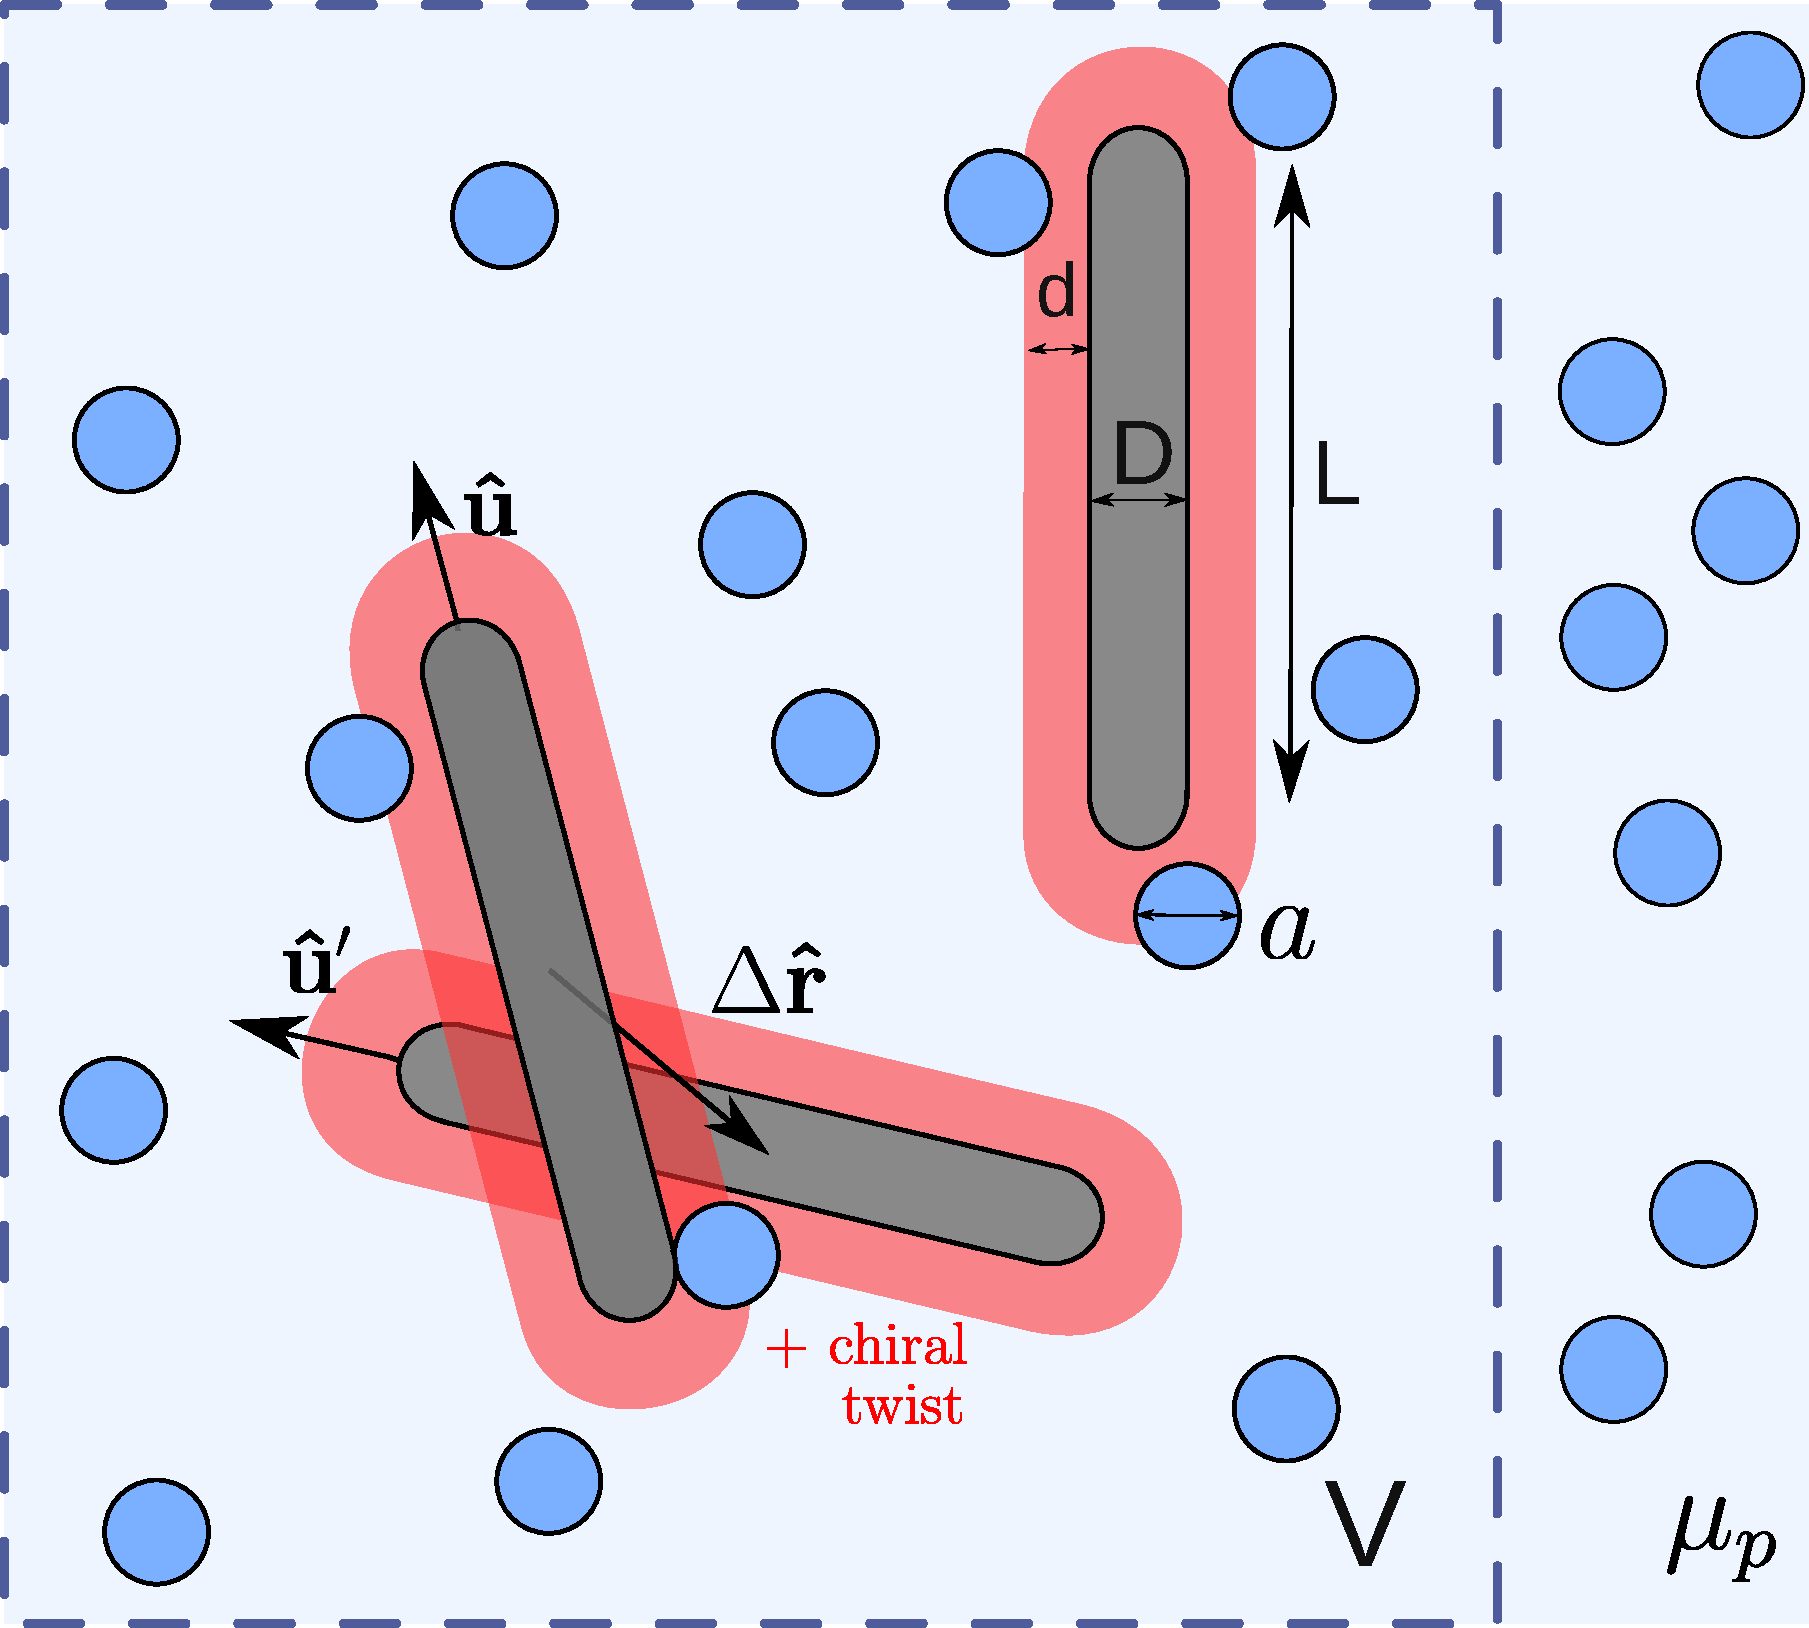
\includegraphics[width = 0.6\columnwidth]{figures/chapter-5/spheromans}
	\caption{ Sketch of the simulation model: hard spherocylinders (grey) mixed with non-adsorbing polymers modeled as penetrable hard spheres (blue) with diameter $a = 2D$ (as depicted here). Overlap of the cores (grey) gives infinite repulsion while overlapping coronae (red zones) favors a twisted pair configuration representing the (chiral) electrostatic forces between {\em fd} rods. The system has a fixed volume $V$ with periodic boundary conditions and connected to a polymer reservoir at constant chemical potential $\mu_p$. }
	\label{sketch}
\end{SCfigure}


We consider a system of $N$ hard-core rigid spherocylinders of length $L$, thickness $D$ and aspect ratio $L/D = 10$. The spherocylinders are a simplified representation of {\em fd} rods that are much thinner ($L/D > 100$) and carry a small degree of backbone flexibility with persistence length $\ell_{p} \gg L$. Since the large particle aspect ratio in combination with backbone flexibility poses considerable limitations on the numerical efficiency of our simulations  we  only consider rigid rods with a relatively short length assuming that the key features of the mesoscopic structures evaluated in this work do not  critically depend on the rod aspect ratio or flexibility. We study these systems (both in bulk and under narrow confinement) by means of Monte Carlo simulations in the semi-grand canonical ensemble ($N,V,\mu_{p},T$) consisting of a system of $N$ rods in a volume $V$ at constant temperature $T$ in osmotic equilibrium with a polymer reservoir at constant chemical potential $\mu_{p}$. The number of polymers  in the system is then a fluctuating quantity with the average polymer concentration controlled by $\mu_{p}$.

\subsection{Depletion interactions}

The spherocylinders are mixed with non-adsorbing polymers that in our model act as penetrable hard spheres. Polymer-polymer interactions are neglected, while the interactions between polymers and spherocylinders are treated as being strictly hard;  the potential energy is infinitely large when a sphere and spherocylinder overlap and zero otherwise. The polymer diameter $a$ is chosen to equal twice that of the spherocylinder ($a = 2D$) because, in that regime, depletants are small enough to realisticly reproduce the depletion effect and big enough to generate long--ranged attraction interactions between the spherocylidners and thus be able to observe intra--lamellar liquid--like order in the resulting smectic compounds. Depletants are treated in an implicit way by means of the algorithm proposed by Glaser {\em et al.} \cite{glaser2015parallel}. More details on the implementation of this algorithm are developed in Section \ref{sec:implicit}.

The simulation box is assigned a fixed volume $V$ and is subjected to periodic boundary conditions (PBC). However, the effective volume of the simulation box is not a critical parameter due to the application of the implicit depletant algorithm, which renders the volume irrelevant as long as it is sufficiently large to avoid any boundary effects affecting the mesogen edges. In practical terms, the depletants are characterized, rather than by their chemical potential $\mu_p$,  by their average packing fraction $\phi_p$; which is defined as the volume fraction in the reservoir fully occupied by spheres. The chemical potential is trivially connected to the polymer packing fraction via:
\beq
\phi_{P} = \frac{\pi D^{3}}{ 6 \Lambda_{p} } e^{\beta \mu_{P}}
\eeq
where $\Lambda_{P}$ denotes the thermal (de Broglie) volume.

 The typical attraction energy between two rods due to polymer depletion can be estimated from free-volume theory \cite{LekkerkerkerTuinier2011} and reads:
 \beq
 U_{\rm r,dep} \sim -\Pi_{P} V_{\rm r, ov}
 \eeq
with $ \Pi_{P} = k_{B} T N_{P}/V$ the (van't Hoff) osmotic pressure of the polymer reservoir and $V_{\rm r, ov}$ the overlap volume  of the depletion layers surrounding each rod which depends on the orientation of each rod.



\subsection{Chiral interactions}

In order to account for both entropical ordering and chiral features, the pair interaction $U_{r}$ between two spherocylinders with solid angles $\oma$ and $\omb$ and centre-of-mass distance $\Delta \bfr$ follows from a combination of short-range steric forces (treated as strictly hard) and electrostatic forces at larger distance. The  interaction potential between a pair of rods depends on centre-of-mass distance vector $\Delta {\bf r}$ and orientation vector $\oma$ of both rods. In our model, the interactions are encapsulated in the following core-shell potential:
\beq
U_{\rm r} (\Delta {\bf r}, \oma, \omb) =
\begin{cases}
\infty & \textrm{if hard cores overlap}\\
U_{\rm twist} & \textrm{otherwise} \\
\end{cases}
\label{urod}
\eeq
The electrostatic interactions between {\em fd} rods give rise to so-called electrostatic twist which is intimately linked to the chirality surface architecture of {\em fd} virus rods. The chiral  potential is commonly expressed in terms of a pseudoscalar form initially put forward by Goossens \cite{goossens}:
\beq
U_{\rm twist} (\Delta {\bf r}, \oma , \omb )=
-\varepsilon_{c} \left ( \frac{D}{\Delta r} \right )^{7}(\oma \cdot \omb)(\oma \times \omb \cdot \Delta \hat{\bf r})
\label{uchiral}
\eeq
where  $\Delta \hat{\bf r} $ denotes a unit vector for the centre-of-mass distance.
 The sign of $\varepsilon_{c}$ defines the microscopic handedness of the rods. Without loss of generality we take $\varepsilon_{c} > 0$ reflecting the right-handedness of {\em fd} rods. The chiral symmetry of the potential is expressed by the pseudoscalar that imparts a sign change upon  inversion $\Delta \hat{\bf r} \rightarrow - \Delta \hat{\bf r}$. In view of its rapid decay with $\Delta r$ the potential is very short-ranged and the rods need to be very close together in order to feel the chiral twist. Thanks to this fast decay, we are able to truncate the interaction range in order to avoid chiral potential calculations between rods that are very far away from each other without affecting the total energy felt by the simulated rods. This truncated range is defined by $d$ in \fig{sketch}. We choose $d=D$ so that the neglected contributions do not possibly exceed $\sim 0.05\varepsilon_c$.

 %For simplicity, we assume that the twisting forces are sufficiently short-ranged (which should be the case at sufficient ionic strength) and do not  continuously vary with the centre-of-mass distance between the spherocylinders, but are only operative if the coronae between the rods overlap (see \fig{sketch}).


%\subsection{Estimation of the depletion strength for two parallel spherocylinders}
%
% The typical attraction energy between two rods due to polymer depletion can be estimated from free-volume theory \cite{LekkerkerkerTuinier2011} and reads:
% \beq
% U_{\rm r,dep} \sim -\Pi_{P} V_{\rm r, ov}
% \eeq
%with $ \Pi_{P} = k_{B} T N_{P}/V$ the (van't Hoff) osmotic pressure of the polymer reservoir and $V_{\rm r, ov}$ the overlap volume  of the depletion layers surrounding each rod which depends on the orientation of each rod. In case the rods are perfectly parallel and at hard-core contact we find a simple analytical result. Ignoring  finite rod size effects we have:
%\beq
%V_{\rm r, ov} = LD^{2} \left [  2 r^{2} \cos^{-1} \left ( \tfrac{1}{2r} \right )  - \tfrac{1}{2} \sqrt{4 r^{2} -1}  \right ]
%\eeq
%with $r = \tfrac{1}{2}(1 + \tfrac{\sigma}{D})$. Rescaling in terms of the polymer packing fraction in the reservoir we find that the maximum depletion strength per rod pair  reads:
%\beq
%  U_{\rm r,dep} \sim - k_{B}T \phi_{P}  \frac{L}{D} \left ( \frac{D}{\sigma} \right )^{3} \left [  2 r^{2} \cos^{-1} \left ( \tfrac{1}{2r} \right )  - \tfrac{1}{2} \sqrt{4 r^{2} -1} \right ]
% \eeq
%For a typical set-up ($\phi_{P} =3$, $\sigma = 2D$ and $L/D=10$) this gives about 15 $k_{B}T$ \red{Please verify this}.

A key parameter in this system is the relative strength of chiral twist versus depletion attraction. These can be combined into a dimensionless parameter $\chi_{T}$ balancing the energy scales associated with twist and depletion as previously discussed:
\beq
\chi_{T} = \frac{\varepsilon_{c}}{U_{\rm r, dep}} \ll 1
\eeq
so that twist becomes more prevalent for larger $\chi_{T}$. It is important to keep in mind that the typical energy due to chiral twist should be small ($ | \varepsilon_{c} | \ll U_{\rm r,dep} $) in order to ensure that the cohesive forces among the rods residing in a droplet are dominated by polymer depletion, with chiral twist playing only a perturbative role.

%\subsection{Rod-wall interactions}

%One possible variation of our model is to confine the rods and polymers in a thin slab of width $h = L$ (see \fig{sketch}). The wall-spherocylinder interactions  are strictly hard, that is, infinite repulsion when the spherocylinder core overlaps with the wall and zero repulsion otherwise. More specifically:
%\beq
%U_{\rm w} (\Delta {\bf r}, \oma) =
%\begin{cases}
%\infty &  | \Delta {\bf r} \cdot {\bf \hat{n}} | < \frac{L}{2}  | \oma \cdot {\bf \hat{n}} | + \tfrac{D}{2} \\
%\infty &   h-  | \Delta {\bf r} \cdot {\bf \hat{n}} | < \frac{L}{2}  | \oma \cdot {\bf \hat{n}} | + \tfrac{D}{2} \\
%0 & \textrm{otherwise}
%\end{cases}
%\label{urodwall}
%\eeq
%with ${\bf \hat{n} }$ denoting the wall normal.

%Polymers are not allowed to overlap with the wall. However, another parameter of the system is the wall depletion range $\sigma_W$ that will take values typically lower than $\sigma$. This strategy is aimed to tune the amount of wetting felt by the tactoids close to the wall, allowing equilibration of partial wetting scenarios. A physical argument for this reduction of the wall depletion range (that in principle would only depend on the size of the depletants), is the variation of the electrostatic forces affecting superficial charges both around the rods and the wall, that may change the effective size of the depletion regions unfavorable for the non-adsorbing polymers.
%The polymers do not have any interaction with the wall, but their centres-of-mass are constrained  to reside within the slab.

\subsection{Simulation details}
Monte Carlo steps conceived from the specifications of the previous sections are performed as follows:

In the initial setup, all rods point along the $z$ direction, their centres of mass are fixed to the XY plane centered in height ($z=L_z/2$) and they are arranged on a hexagonal lattice inside a circular domain. During the relaxation from the initial configuration, we randomly apply single--particle moves: translations within the volume and rotations around arbitrary axes. To decide if a trial move is accepted, we first check for overlaps with other colloids and with depletants. If no overlap takes place, the variation in the chiral energy is computed and the Metropolis acceptance criterion is used to decide whether the move is energetically favorable. If the move induces a loss in energy, it is accepted; otherwise it will be accepted with probability $\sim\exp{\left[-\beta(U_{new}-U_{old})\right]}$

The step size for the spherocylinder translations and rotations are chosen adaptively such as to maintain an average acceptance ratio of about 30 \%. The MC code is optimized using cell-linked list routines that significantly reduce the number of overlap checks between rod-rod and rod-polymer pairs involved in each MC step. We keep a rectangular box shape with $L_{x} = L_{y} =L_{z}$ and periodic boundary conditions (PBC) in all directions.

%Depending on the polymer size and concentration the system will either evolve into a liquid drop ("tactoid") or  will retain its crystalline inner structure (expected for `sticky' depletion forces induced by small polymers, $\sigma = D$).
We monitor the total overlap volume of the depletion layers $V_{\rm ov}$ and the total twist energy $\mathcal{U}  = \sum_{i}\sum_{j<i}U_{\rm twist}$ to gauge whether the drop has reached its equilibrium state.

We plan to focus on two different systems:

\begin{itemize}
\item  Small polymers with $\sigma = D$ imparting short-ranged attractions. The initial configuration is a square monolayer of perfectly parallel rods ordered into a hexagonal lattice. Without confinement, the cluster will equilibrate into a membrane with  fluid order. In. our simulations we fix the polymer concentrations $\phi_{P}=1$ and $N=2000$. Note that small changes in $\epsilon_{c}$ may have large consequences for the way the droplet expresses chiral twist. At weak twist ($\varepsilon_{c} < ****$), the membrane remains circular in shape with twist showing up at the membrane edges while the membrane center remains largely unperturbed. At strong twist ($\varepsilon > ****$) the membrane may transform into a twisted ribbon. \red{The first indication of such a change of droplet morphology can be observed in \fig{samples} a and c.   Bigger systems ($N=2000$) spontaneously form ribbon-shaped protrusions around a circular central body which resembles the onset of twisted ribbon formation.  }.  Next we introduce confinement and re-assess the droplet shape and internal structure and compare with experimental observations.

\item Large polymers with $\sigma = 2 D$ imparting long-ranged attractions. We start from the same monolayer crystal which will equilibrate into a liquid tactoid in bulk \cite{kuhnhold2022structure}. Gradually increasing the confinement (at $R_{2} > h$ with $R_{2}$ the minor curvature radius of an unconfined tactoid \cite{kuhnhold2022structure})  will lead to squeezed tactoids which  develop a distinct biaxial shape. Introducing twist may lead to further morphological changes. We may correlate droplet size ($N$) with droplet aspect ratio for the strongly confined case compared to the 3D case studied in \cite{kuhnhold2022structure}.

\end{itemize}

%\begin{itemize}
%\item  Small polymers with $\sigma = D$ imparting short-ranged attractions. The initial configuration is a square monolayer of perfectly parallel rods ordered into a hexagonal lattice. Without confinement, the cluster will equilibrate into a membrane with  fluid order. In. our simulations we fix the polymer concentrations $\phi_{P}=1$ and $N=2000$. Note that small changes in $\epsilon_{c}$ may have large consequences for the way the droplet expresses chiral twist. At weak twist ($\varepsilon_{c} < ****$), the membrane remains circular in shape with twist showing up at the membrane edges while the membrane center remains largely unperturbed. At strong twist ($\varepsilon > ****$) the membrane may transform into a twisted ribbon. \red{The first indication of such a change of droplet morphology can be observed in \fig{samples} a and c.   Bigger systems ($N=2000$) spontaneously form ribbon-shaped protrusions around a circular central body which resembles the onset of twisted ribbon formation.  }.  Next we introduce confinement and re-assess the droplet shape and internal structure and compare with experimental observations.
%
%\item Large polymers with $\sigma = 2 D$ imparting long-ranged attractions. We start from the same monolayer crystal which will equilibrate into a liquid tactoid in bulk \cite{kuhnhold2022structure}. Gradually increasing the confinement (at $R_{2} > h$ with $R_{2}$ the minor curvature radius of an unconfined tactoid \cite{kuhnhold2022structure})  will lead to squeezed tactoids which  develop a distinct biaxial shape. Introducing twist may lead to further morphological changes. We may correlate droplet size ($N$) with droplet aspect ratio for the strongly confined case compared to the 3D case studied in \cite{kuhnhold2022structure}.
%
%\end{itemize}



\section{Results}


\begin{figure}
\begin{center}
\includegraphics[width= .8\columnwidth]{figures/chapter-5/samples}.
	\caption{Top and front views of membrane-shaped tactoids of chiral rods mixed with non-adsorbing polymer formed in bulk. Color indicates the enclosed angle between each individual rod and membrane normal, from black $\varphi = 0$ to yellow $\varphi = \frac{\pi}{2}$. Shared parameters are $a = 2D$, $\ell = 10$ and $N = 500$. For the cases where vertical fluctuations are (not) allowed, $\phi_P=0.25D^{-3}$ ($\phi_P=0.175D^{-3}$).(a) Low chirality regime. (b) Strong chirality regime showing a cascade of multi-core membranes.}
 \label{multidomain}
\end{center}
\end{figure}


\begin{figure}
\begin{center}
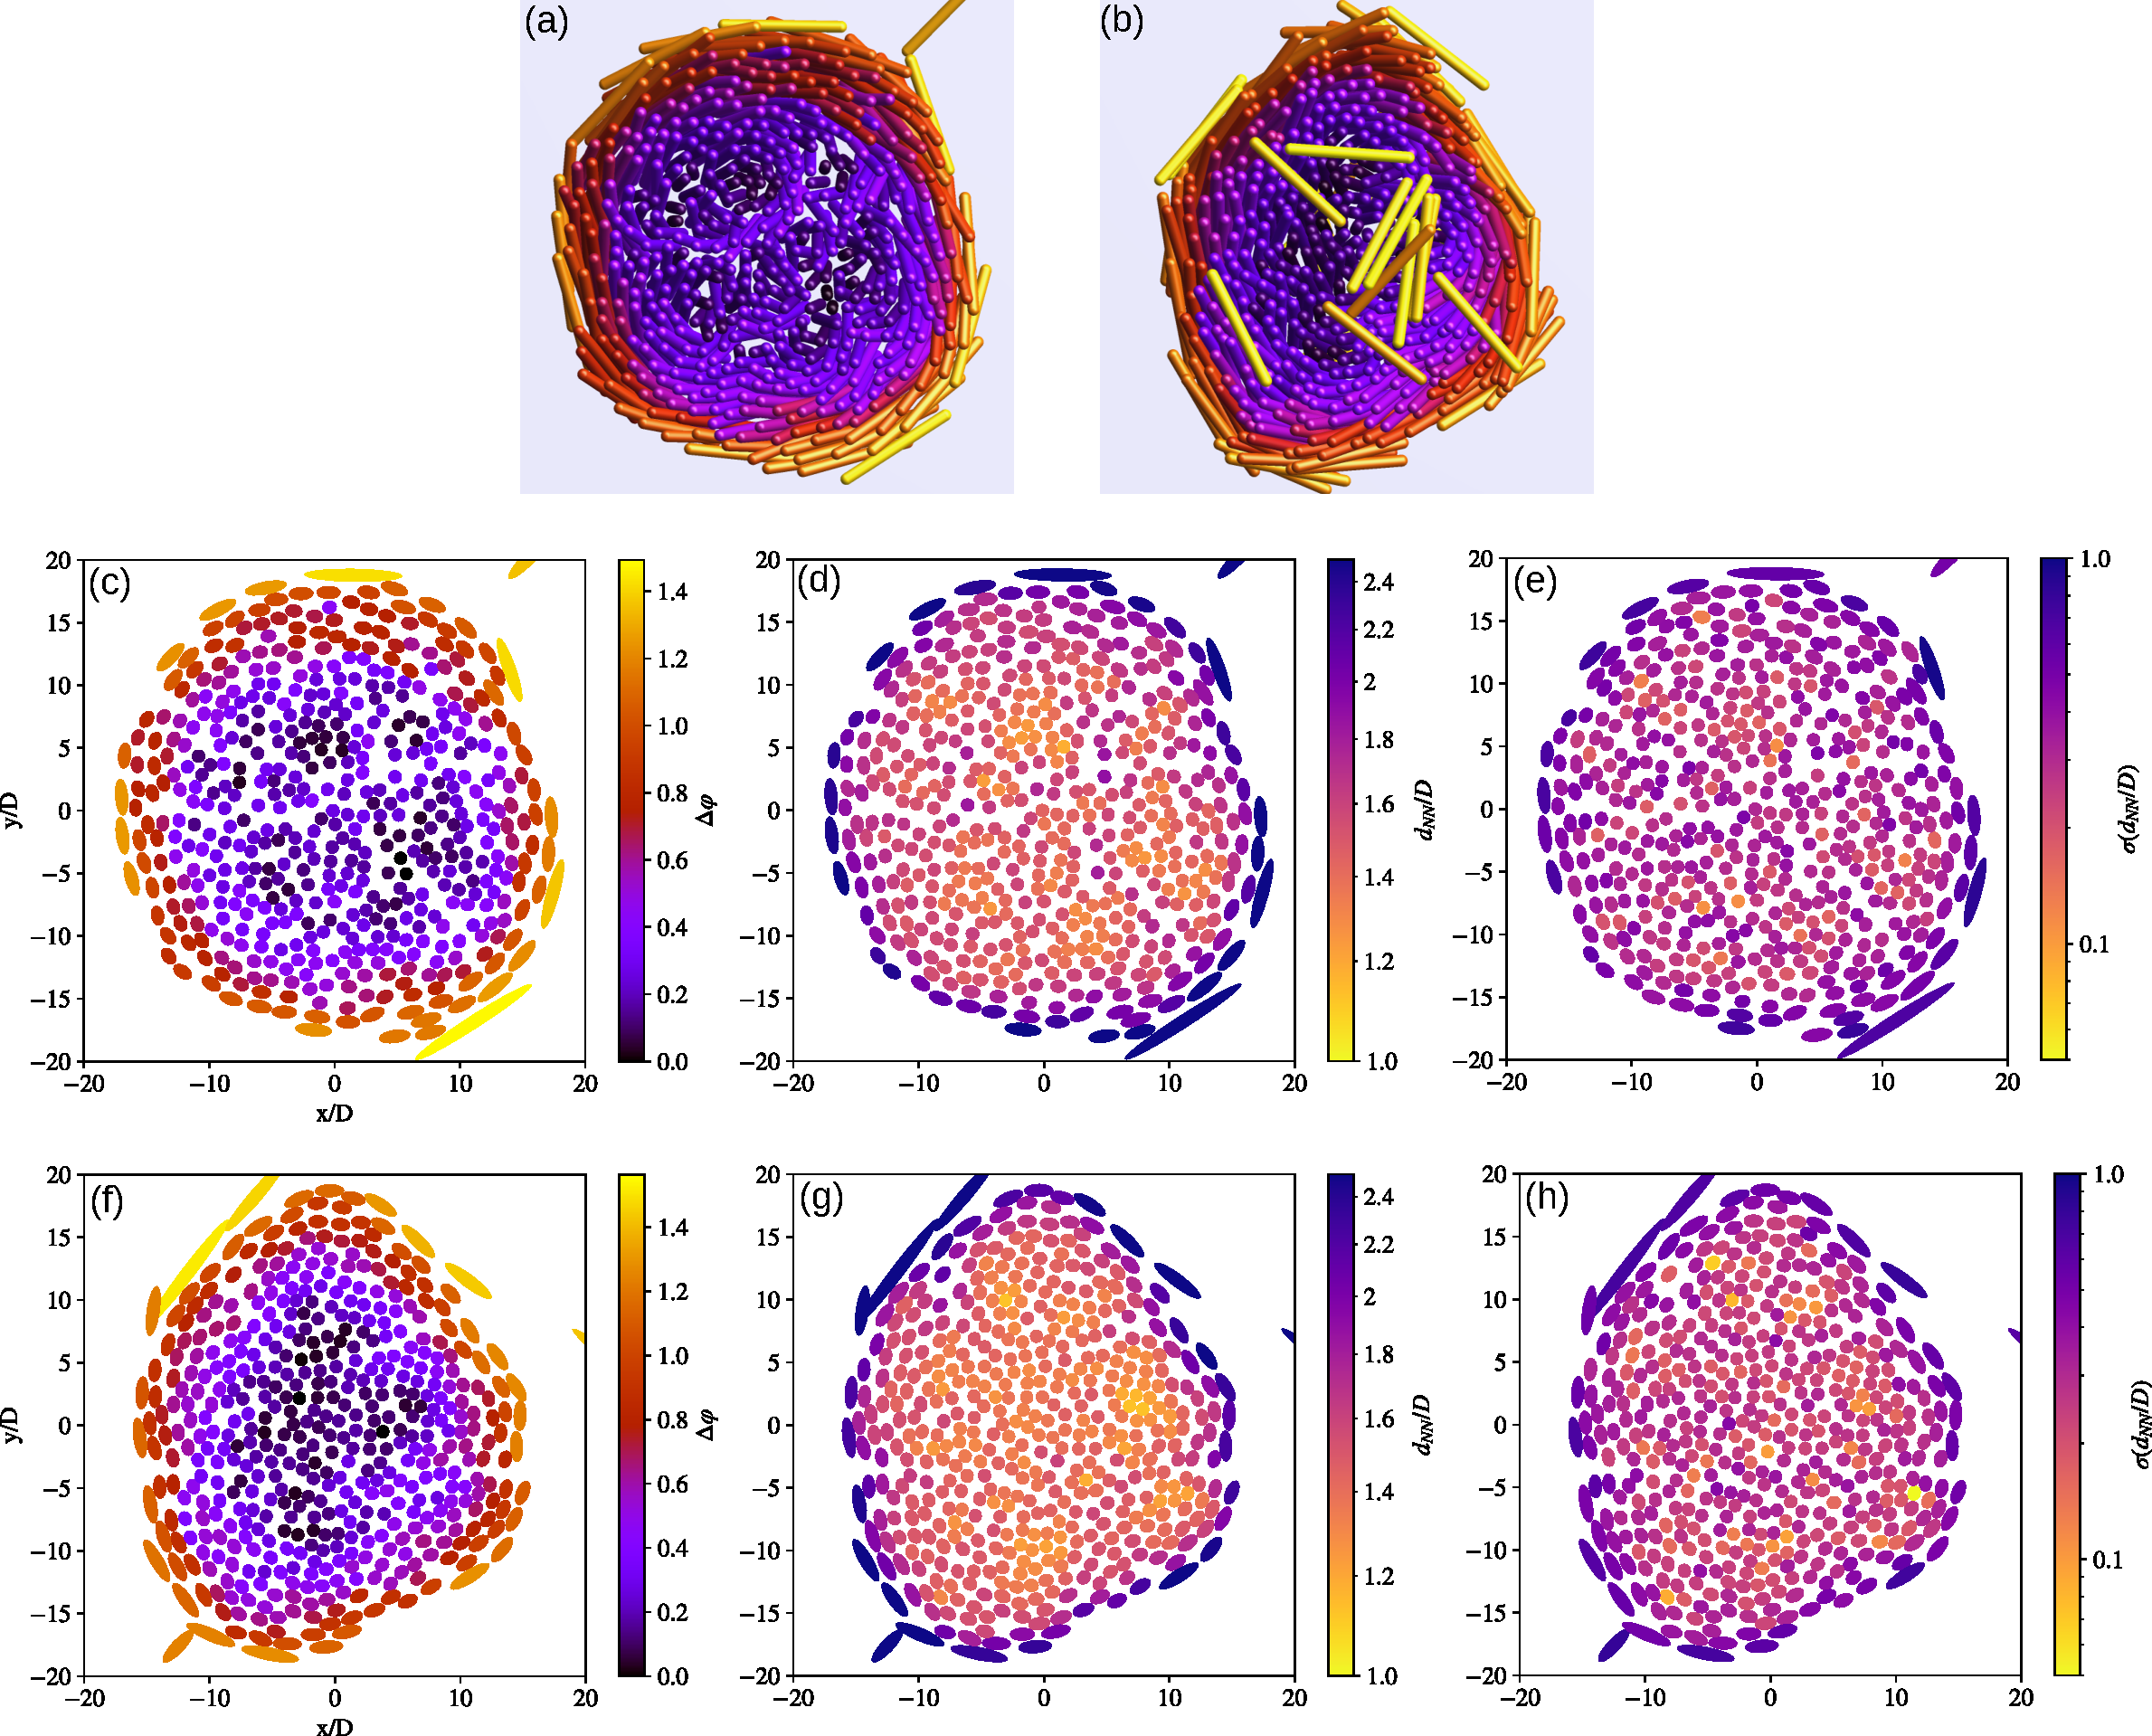
\includegraphics[width= \columnwidth]{figures/chapter-5/crystallinity_11}.
	\caption{ \label{crystal11} Crystallinity of membrane-shaped tactoids of chiral rods mixed with non-adsorbing polymer formed in bulk. Top row: 3D depiction of the system (a) without vertical fluctuations and (b) with vertical fluctuations. Middle and bottom rows: corresponding horizontal sections along the plane generated from a 2D linear regression of the centers of mass of the rods. Upright (untwisted) rods look like disks in this view, while tilted rods appear as ellipses. Color scales indicate: (a)-(c), (f): enclosed angle between the direction of each individual rod and the overall average direction; (d), (g): average distance between each individual rod and its six nearest neighbours; and (e), (h): nearest neighbour distance's standard deviation. Shared parameters are $a = 2D$, $\ell = 10$, $N = 500$ and $\varepsilon_c=11$. For the case where vertical fluctuations are (not) allowed, $\phi_P=0.25D^{-3}$ ($\phi_P=0.175D^{-3}$).}
\end{center}
\end{figure}


\begin{figure}
\begin{center}
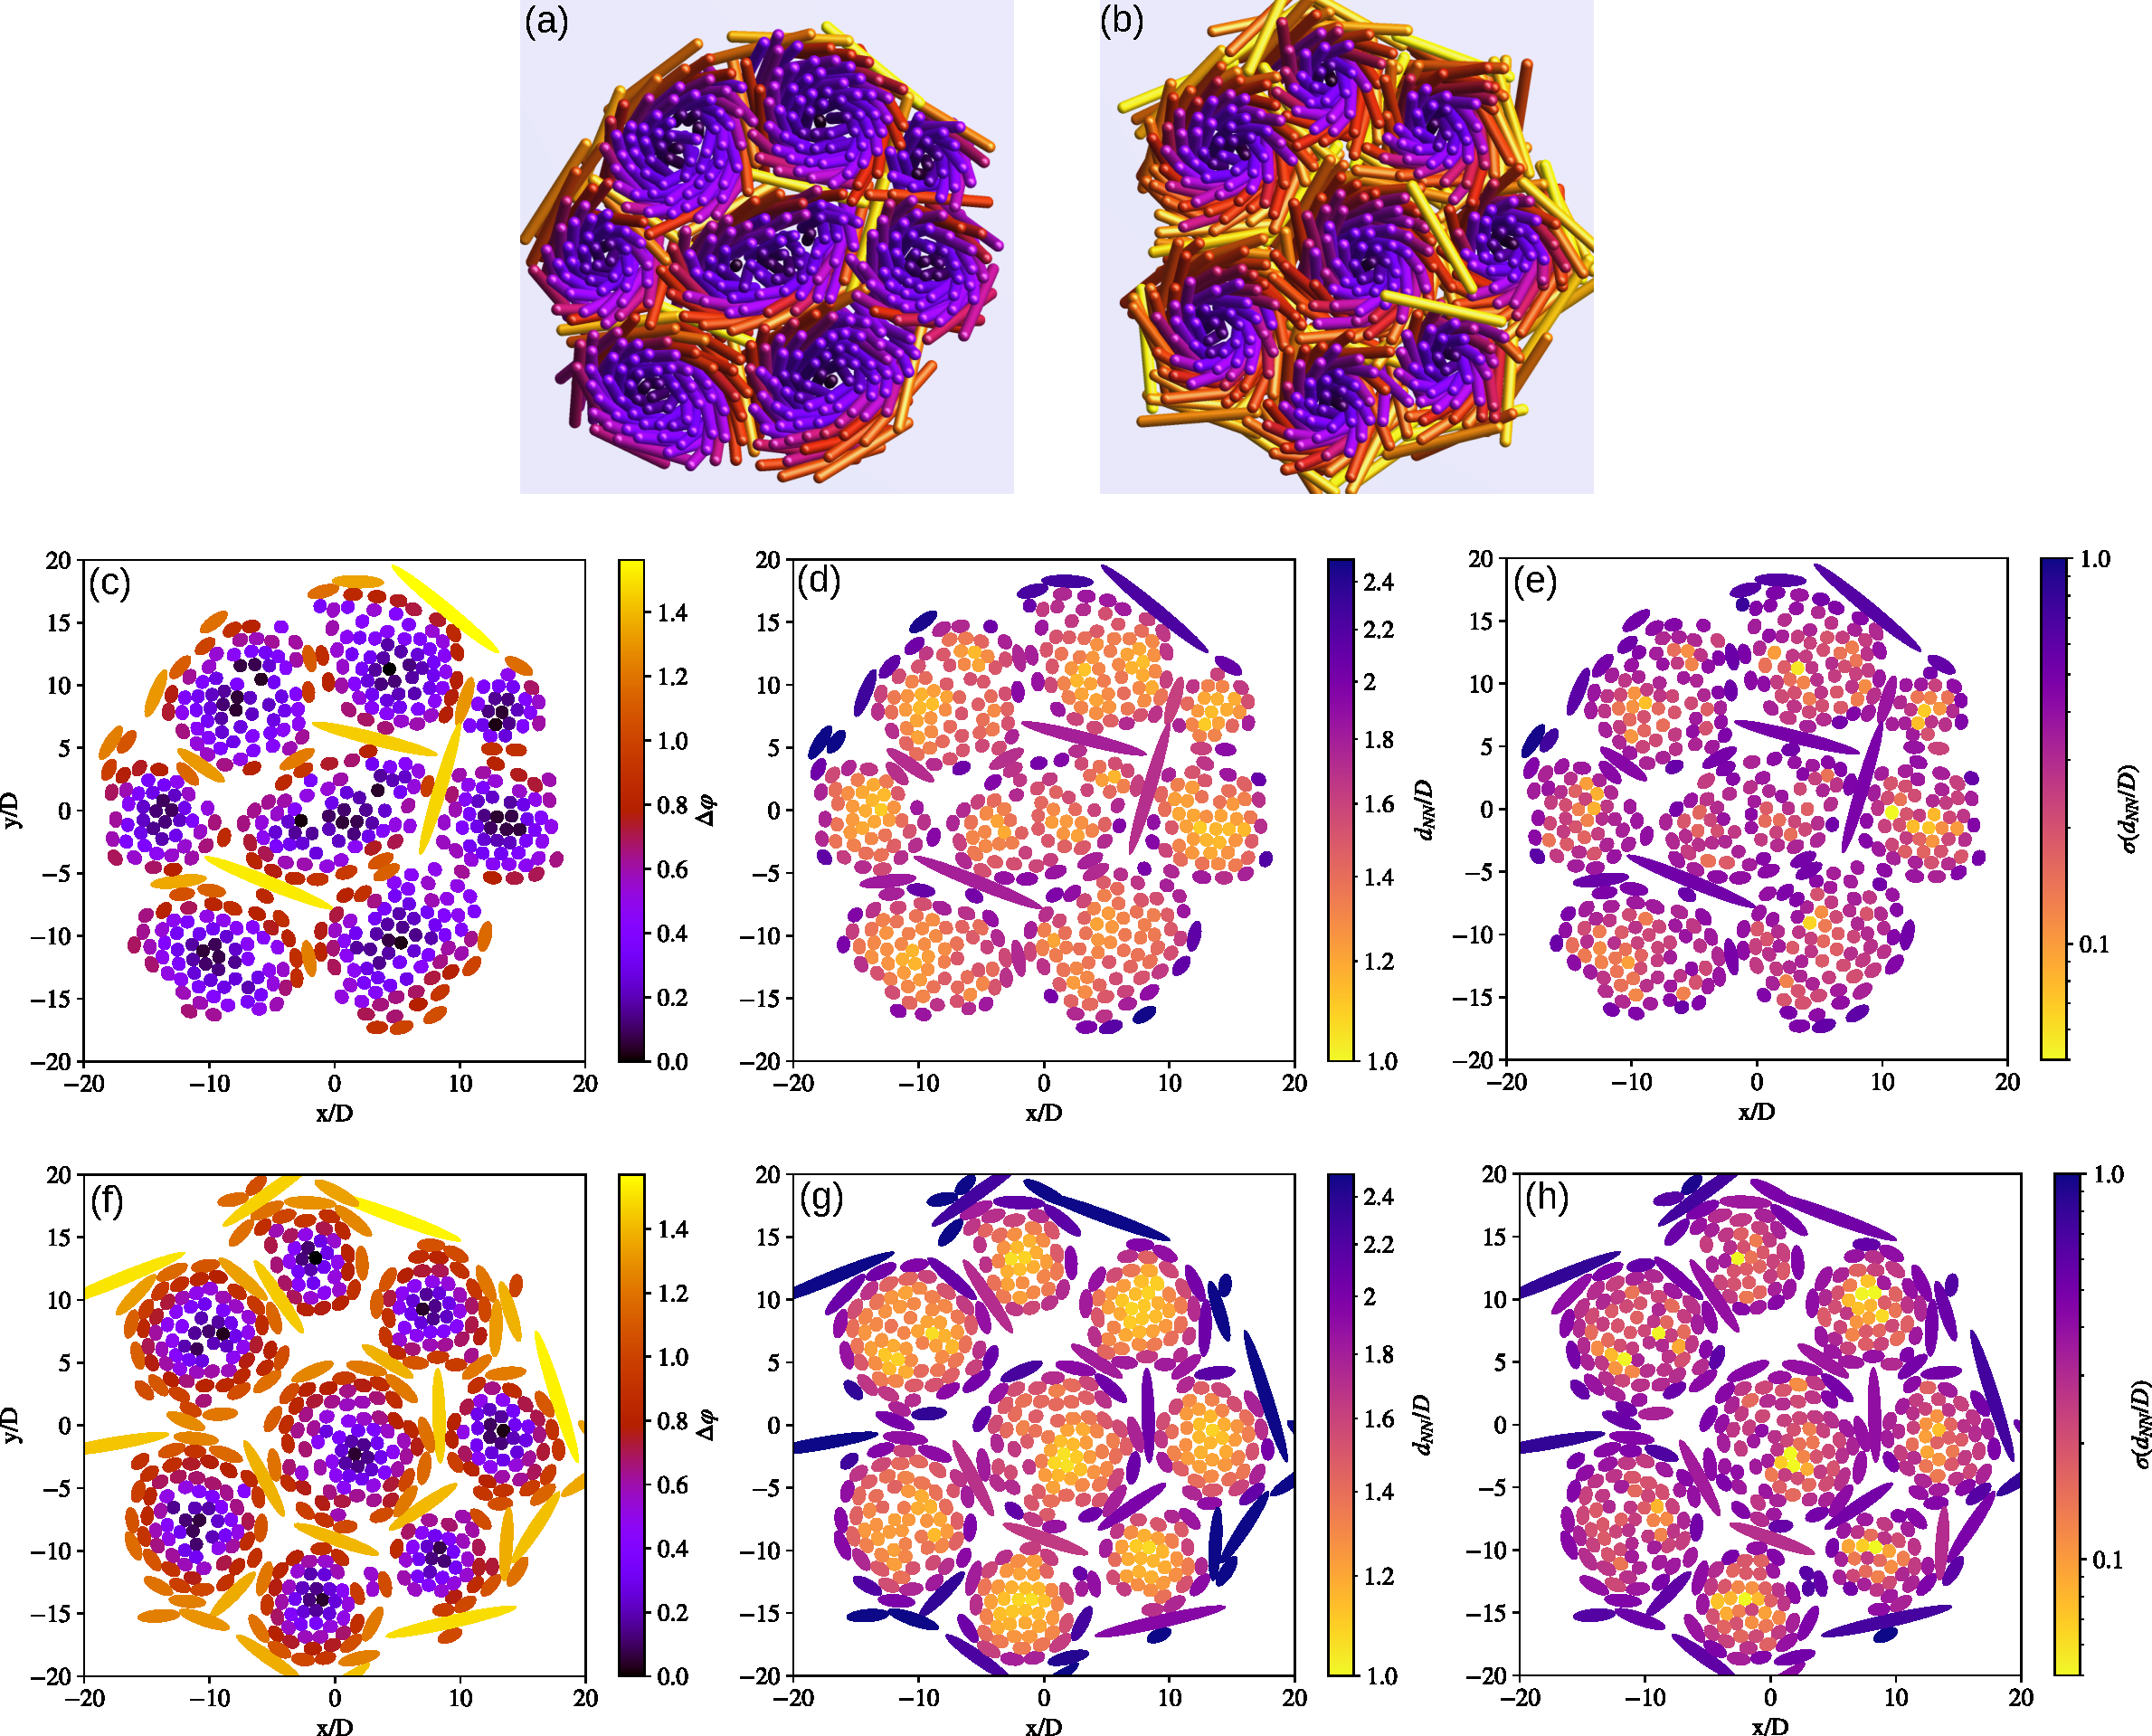
\includegraphics[width= \columnwidth]{figures/chapter-5/crystallinity_16}.
	\caption{ \label{crystal16} Crystallinity of multi-domain membrane-shaped tactoids of strongly chiral rods mixed with non-adsorbing polymer formed in bulk. What is illustrated in this figure is equivalent to \fig{crystal11} except for the chosen chirality regime ($\varepsilon_c=11$ in \fig{crystal11}, $\varepsilon_c=16$ in this figure).}
\end{center}
\end{figure}


\begin{figure}
\begin{center}
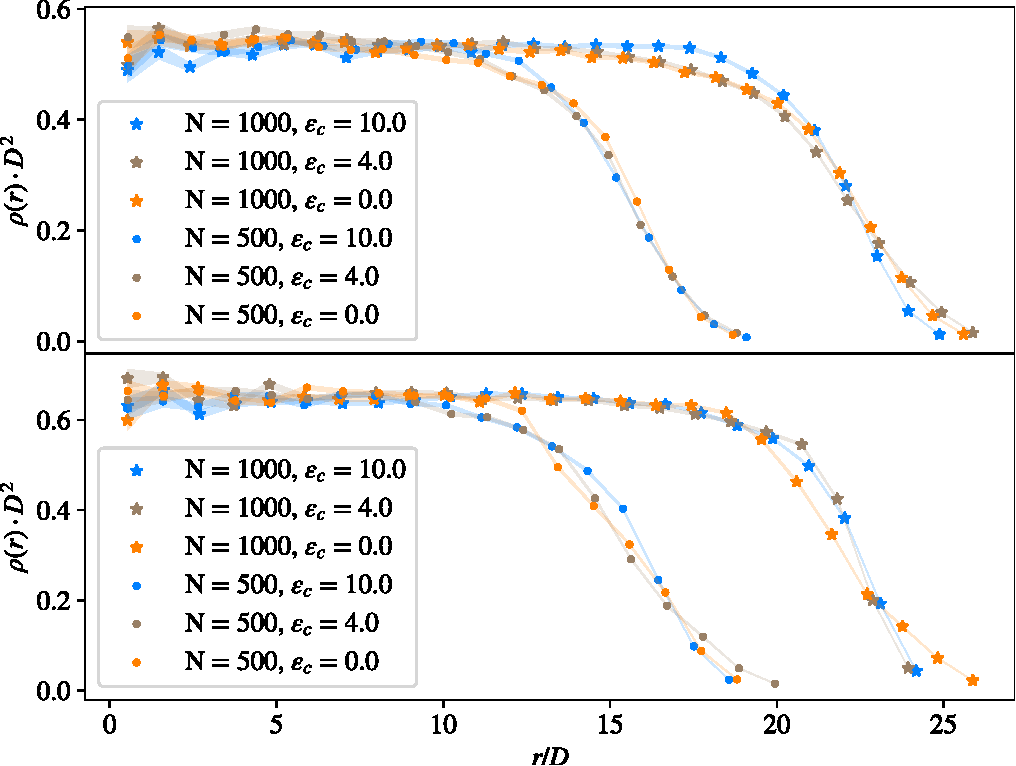
\includegraphics[width= .9\columnwidth]{figures/chapter-5/density}.
	\caption{Rod number density profile of membrane-shaped tactoids of chiral rods mixed with non-adsorbing polymer formed in bulk. Top: without vertical fluctuations. Bottom: with vertical fluctuations. For all cases, $a = 2D$. For the cases where vertical fluctuations are (not) allowed, $\phi_P=0.25D^{-3}$ ($\phi_P=0.175D^{-3}$). } % TODO: explain more.
 \label{density}
\end{center}
\end{figure}


\begin{figure}
\begin{center}
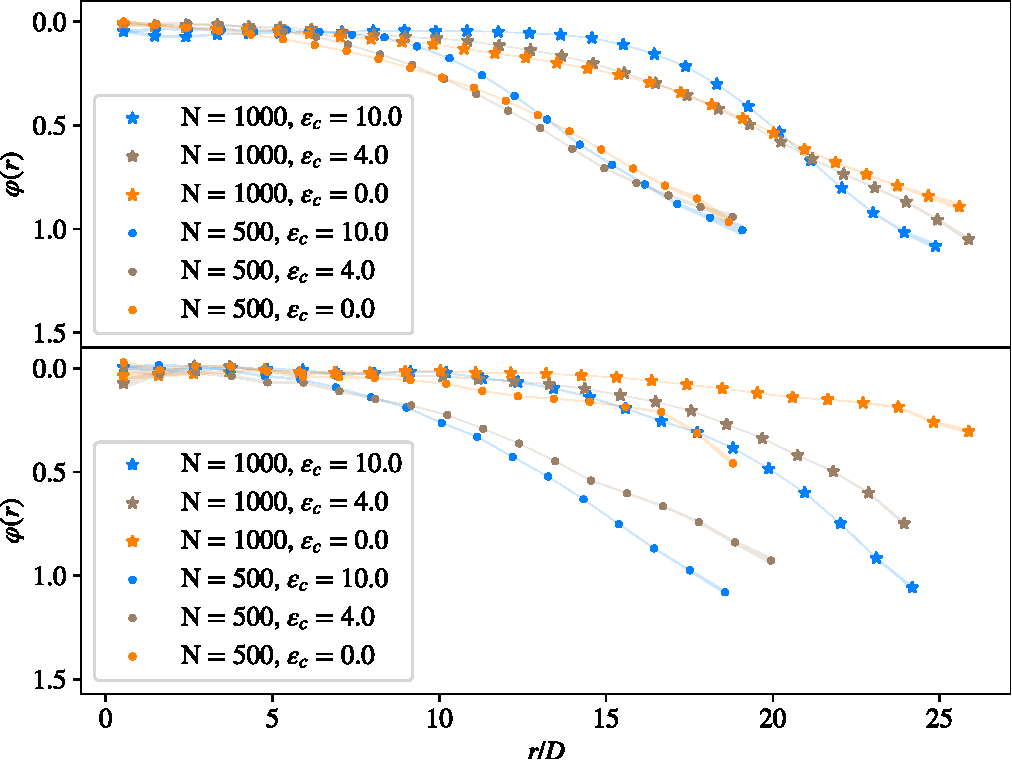
\includegraphics[width= .9\columnwidth]{figures/chapter-5/twistprofile}.
	\caption{Twist angle profile of membrane-shaped tactoids of chiral rods mixed with non-adsorbing polymer formed in bulk. Top: without vertical fluctuations. Bottom: with vertical fluctuations. For all cases, $a = 2D$. For the cases where vertical fluctuations are (not) allowed, $\phi_P=0.25D^{-3}$ ($\phi_P=0.175D^{-3}$). } % TODO: explain more.
 \label{twangle}
\end{center}
\end{figure}


\begin{figure}
\begin{center}
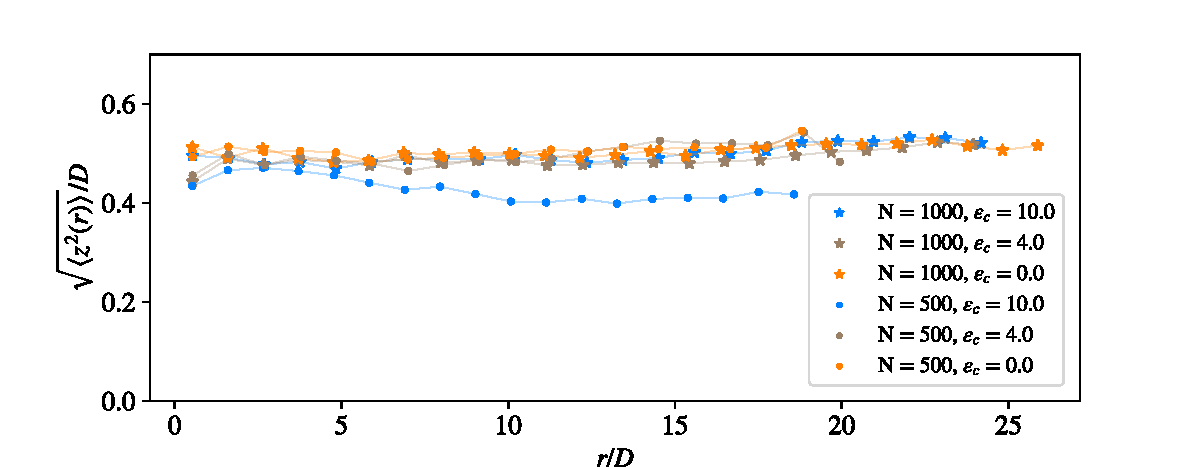
\includegraphics[width= \columnwidth]{figures/chapter-5/zstd}.
	\caption{Vertical fluctuations as a function of the distance to the center of 3D membrane-shaped tactoids of chiral rods mixed with non-adsorbing polymer formed in bulk, $a = 2D$, $\phi_P=0.25D^{-3}$. } % TODO: explain more.
\end{center}
\end{figure}





\section{Theory for twisted membranes}




\begin{SCfigure}
\includegraphics[width= 0.4 \columnwidth]{figures/chapter-5/membrane_sketch}.
\caption{ \label{memsnap} Schematic structure (top and front view) of a twisted smectic membrane of radius $R_{m}$ composed of strongly chiral spherocylinders with aspect ratio $\ell = 10$ mixed with non-adsorbing polymers (not shown) providing strong side-to-side depletion attraction between the rods.  The top graph depict the top view, the lower one a side view of the membrane. The director twist, expressed by the twist angle $\varphi$, is zero at  the membrane  core $\bn _{\rm core} = \bz$ and increases concentrically with radius $R$.}
\end{SCfigure}




 To complement our simulations results we now develop a theory for twisted membranes by focussing on two distinct morphologies that have been observed in experiment, namely half-skyrmion-type membranes and twisted ribbons. In both cases, the twisting of the rods occurs in both principal directions of the membrane (double twist), whereas the cholesteric phase exhibits unidirectional twist. Somewhat confusingly, double twist may also refer to the case of {\em chiral ribbons} in which the membrane itself is wrapped 
in a helical fashion thus exhibiting non-zero mean curvature \cite{green1936equilibrium,chopin2016roadmap}. Although these chiral ribbons have also been observed in {\em fd} polymer mixtures under cetain conditions \cite{Gibaud2012} but we will not consider this particular case in our model.
 
 
 Let us begin by recalling the well-known Frank-Oseen elastic energy of the general case of a bulk chiral liquid crystal for and arbitrary nematic director field $\bn$ in three spatial dimensions:
\begin{align} 
F = & \frac{1}{2} \int d \bfr \left [ K_{1} (\nabla \cdot \bn)^{2}  + K_{2} (\bn \cdot \nabla \times \bn + q_{0})^{2}  +   K_{3} (\bn \times \nabla \times \bn)^{2} \right ]  
\end{align}
with $K_{1}$, $K_{2}$ and $K_{3}$ respectively denoting the splay, twist and bend elastic moduli.   The inverse  pitch  $q_{0}$ quantifies the chiral strength of the particles in the liquid crystal. 


 For the specific case of a cylindrically symmetric, twisted membrane depicted in\fig{memsnap}
  with radius $R_{m}$ we may invoke a cylindrical geometry  with radial coordinate $0<R< R_{m}$ and angle $\alpha$.  Deformations from a uniform director field in which case $\bn = \bz$ are assumed to be concentric and can be described as:
 \beq
 \bn = \cos \psi (R) \cos  \varphi(R) \bz + \cos \psi (R) \sin \varphi(R) \bal + \sin \psi(R) \bars
 \label{tilt}
 \eeq
in terms of a twist angle  $ \varphi $ denoting a twist deflection of the rods with respect to the membrane normal and $\psi$ a splay deformation along the membrane radial vector (see \fig{memsnap}).   We the local rod density within the membrane to be uniform so that the one-body density reads $\rho(R, \bw)  = \rho_{0}f(R,  \bw)$, in terms of the rod number density $\rho_{0}$ denoting the number of rods per area unit, and a three-dimensional rod unit vector $\bw$ distributed along the local director obeying an a priori unknown distribution $f$. The twist-bend elastic free energy  takes the following form \cite{barry_jpcb2009,wensink2018elastic}:
\begin{align}
 F_{el}  &= \int  d \brr \left [ K_{2} \left ( \partial_{R} \varphi + \frac{\sin 2 \varphi}{2R} + q_{0} \right )^{2}  + K_{3}\frac{ ( \sin \varphi )^{4}}{R^{2}} \right   ]
\label{fmem}
\end{align}
with $\int d {\bf R} = 2 \pi \int_{0}^{R_{m}} R dR $ in circular coordinates for a membrane with radius $R_{m}$.
 The  elastic moduli for the membrane are distinctly different from those of a ulk liquid crystal and will be specified in the next section. We remark that these elastic moduli are strictly 2D quantities with dimension energy.  


In an earlier version of our theory \cite{wensink2018elastic} the effect of depletion attraction due to the non-adsorbing polymer can be described in terms of a simple free energy 
\beq
F_{dep}  \sim U_{0} \int d \brr  (\sin \varphi )^{2}  + {\rm cst}
\eeq
where $U_{0}$ is a tilt energy density (per unit area) related to the osmotic pressure of the polymer reservoir and polymer radius of gyration. The simple sine squared contribution is chosen here for simplicity and is in line with de Gennes' original treatment of twist expulsion towards the edges or around defects of smectic layers in analogy with superconductors \cite{gennes-prost, barry_jpcb2009}. It captures the basic trend that the local director tilting away from the membrane normal compromises the free volume experienced by the non-adsorbing polymer  thereby inducing a free energy penalty. In our theory, out-of-plane fluctuations of the rod centre-of-mass away from the 2D plane are not included, but this can be done so on a simple mean-field level \cite{kang_sm2016}.
Ignoring the curvature terms  $R \rightarrow \infty $ and considering a smectic layer on an infinite half-plane enables an analytical minimisation of the free energy in terms of the twist penetration depth $\lambda_{t}  =  \sqrt{K_{2}/a} $ \cite{gennes-prost,barry_jpcb2009}. For the circular membrane, a simple simulated-annealing Monte Carlo algorithm can be employed to minimise the free energy with respect to the twist angle $\varphi(R)$ for any given triplet of length scales, namely the bulk cholesteric pitch $q_{0}^{-1} $, twist penetration depth $\lambda_{t} $ and membrane radius $R_{m}$. With the twist elastic modulus and chiral amplitude being microscopically defined \eq{kexp} a simple one-parameter fitting procedure can be used to determine the depletion strength $a$ and the twist penetration depth $\lambda_{t}$. 



 The main features we established from the numerical results \cite{wensink2018elastic} are the following:  (i) the twisting becomes more pronounced toward the membrane edge when the twist penetration depth becomes shorter, as expected,  but also when membrane size grows larger. (ii) Increasing the pitch $q_{0}$  enhances the maximum twist angle while keeping the overall shape of the twist angle profile largely unchanged. (iii) The local splay angle remains negligibly small  across the membrane so that the omission of splay effects seems fully justified.




\subsection{Scaling results for the elastic moduli for a fluid membrane}

Using second-virial theory combined with a Gaussian approximation for the orientation probability of the rods within the membrane one can estimate the leading-order contributions of the torque-field, splay, twist and bend elastic constants of a membrane, respectively:
\begin{align}
  K_{1}   & \sim  \frac{17 \rho_{0} \ell^{2}}{24} = \frac{17}{2} K_{2}   \nonumber \\ 
 K_{2}  & \sim  \frac{\rho_{0} \ell^{2}}{12}   \nonumber \\ 
 K_{3} &\sim  \frac{1}{4} K_{2}
  \label{kexp}
\end{align}
Note that the membrane moduli have unity ${\rm N \cdot m}$ (the 3D moduli would be expressed in Newtons) and $\rho_{0} = ND^{2}/A$ refers to planar density of rods with diameter $D$, aspect ratio $\ell = L/D$ and membrane area $A$. The results suggest that the moduli of rodlike particle confined to a membrane are quite different from those of of 3D bulk nematic fluid, at least for strongly elaongated rods experiencing strong nematic order.  In the limit of asymptotic alignment, the splay-to-twist ratio of a bulk fluid  \cite{odijkelastic}  was predicted to scale as $K_{1}/K_{2} \sim 3 $ whereas a much higher ratio $K_{1}/K_{2} \sim 17/2$ is found for the membrane. The bend-to-twist ratio for a hard rod nematic fluid was found to be proportional to the degree of nematic alignment $K_{3}/K_{2} \sim \sigma \gg 1$ \cite{odijkelastic} where $\sigma$ is steered by the rod concentration.  The curvature-to-twist elasticity of a membrane turns out to be smaller than unity $K_{3}/K_{2} \sim 1/4$ and independent of the rod concentration.  In other words, rods confined to a membrane experience a much stronger resistance to splay fluctuations whereas  bend fluctuations are far less penalised compared to a 3D nematic fluid.  Since the splay modulus is about an order of magnitude larger than the twist elasticity, we expect director deformations whereby rods tilt along the radial vector of the membrane to be of marginal importance and  will be ignored.  





\subsection{Chiral twist }

The pitch $q_{0}$ of a twisted membrane can be estimated by considering a weakly chiral pair potential $U_{c}$ described by some arbitrary but short-ranged spatial decay function $g(r)$ describing the range over which chiral forces interact and chiral amplitude $\varepsilon_{c} $ much smaller than the thermal energy. This potential takes the following generic form \cite{goossens1971}:
\beq
U_{c} \sim  \varepsilon_{c} g( r)(\bwa \times \bwb \cdot   \bx) (\bwa \cdot \bwb)
\label{uchi}
\eeq
From this, we may compute the so-called torque-field constant exerted by the chiral potential \cite{wensink2018elastic}:
\beq
K_{t}   \sim -\rho_{0}^{2}  \bar{\varepsilon}_{c} 
\eeq
in terms of an integrated chiral amplitude  $\bar{\varepsilon}_{c}$ which is  {\em different} from that of a  3D cholesteric system as it implicitly encodes the geometric confinement given that $\bdr$ is a 2D vector:
\beq
 \bar{\varepsilon}_{c}  =  \varepsilon_{c} \int d \bdr | \bdr \cdot \bx |    g( r)
 \eeq
 which has units energy times volume ($k_{B}T \times D^{3}$). The chiral potential drives the twisting of the membrane and $K_{t}$  provides an explicit link between the effective torque-field and the range and amplitude  of the chiral pair potential between a pair of  rods. We remark that the above mean-field treatment will be less adequate for strongly chiral amplitudes $\varepsilon_{c} \gg k_{B}T$. A common choice for $g(r)$ is a short-ranged power law $g(r) = 1/r^{7}$ but  long-ranged forms such as a square-well (SW) potential could be conceivable as well \cite{wensinkjackson}. Taking the power law featuring in \eq{uchiral} we obtain $\bar{\varepsilon}_{c} = \varepsilon_{c} D^{3}$.  From this we find a {\em microscopic} expression for the typical equilibrium  pitch of the membrane $q_{0} = K_{t}/K_{2}$ that further depends on the in-plane rod density $\rho_{0}$ and rod aspect ratio $\ell = L/D$:
 \beq
 q_{0} \sim \frac{12 \rho_{0} \bar{\varepsilon_{c}}}{ \ell^{2}}
 \label{qzero}
 \eeq
 While for the single-twisted cholesteric phase the twist angle increases linearly  $\varphi(z) = q_{0} z$ at each position $z$ along the helix axis, the angle will be strongly non-linear with radius $R$ in case of the twisted membrane, in particular if the twist penetration length $\lambda_{t}$ is small \cite{wensink2018elastic}.   
 


\subsection{Effect of depletants and twist penetration length}

Kang et al. \cite{kang_sm2016} have proposed a more sophisticated expression for the effect of the depletion attraction on the twist angle via the local membrane height $h = (L/2) \cos \varphi$: 
\begin{align}
F_{dep}  \sim & 2 n_{p} a k_{B}T \left [ \int  d {\bf R} \sqrt{ 1 + (\nabla h)^{2} } + \oint d {\bf l} h \right ]
\label{fdep1}
\end{align}
with $n_{p}$ the polymer reservoir pressure and $a$ the polymer radius of gyration. The last contribution is identified a line tension generated by depletion forces between rods. Combining this with the elastic part of the 
\eq{fmem} we find the following free energy for a membrane with radius $R_{m}$:
\begin{align}
\frac{ F}{K_{2}}  &\sim \int  d \brr   \left [  \left ( \partial_{R} \varphi + \frac{\sin 2 \varphi}{2R} + q_{0} \right )^{2}  + \frac{K_{3}}{K_{2}}\frac{ ( \sin \varphi )^{4}}{R^{2}} \right . \nonumber \\ 
& \left .  + \lambda_{t}^{-2}    \sqrt{ 1 + (\partial_{R} h)^{2} }   \right ]  + 2 \pi  \lambda_{t}^{-2} R_{m} h(R_{m})
\label{fmem1}
\end{align}
with $\int d {\bf R} = 2 \pi \int_{0}^{R_{m}} R dR $ in circular coordinates. The line tension contribution drops with increasing twist at the edges and  becomes zero if the rods are twisted perpendicular to the membrane normal $\varphi(R_{m}) = \pi/2$. 
The twist penetration length is given by $\lambda_{t} = \sqrt{K_{2}/2  n_{p} a k_{B}T}$ which, using \eq{kexp} leads to a compact expression depending on quantities known from experiment such as the in-plane rod density (assumed uniform across the membrane), rod-polymer size ratio $D/a$, rod aspect ratio $\ell$ and the reservoir polymer concentration $n_{p}$: 
\beq
\frac{\lambda_{t}}{D} = \sqrt{\frac{\rho_{0} \ell^{2} }{24  (n_{p} a^{3}) (D/a)^{2} }}
\eeq
Taking typical numbers from our simulation ($\ell \sim 10$, $\rho_{0} \sim 0.5$, $D/a=2$ and $n_{p}a^{3} \sim 0.2$) we find that that the twist penetration length is only a few times the rod diameter, i.e. $\lambda_{t} \sim 2 D$. This is broadly in line with the twist angle profiles  in \fig{twangle} where the twist expulsion at the edge was found to extend over a typical distance  of about $\sim 5D$.  
For {\em fd} rods a much larger value is found primarily because they are longer than our rods ($\ell \sim 130$). The predicted value $\lambda_{t} \sim 20 D$ is roughly line with the experimentally measured value of about half a rod length   depending on the polymer concentration that was used to stabilize the membranes \cite{barry_jpcb2009}.

In Ref. \cite{kuhnhold2022colloidal} a simple trial form was used to fit the simulation data:
\beq
\varphi(R) = \varphi_{0} \left ( \frac{R}{R_{m}} \right )^{\alpha} 
\eeq
with $\varphi_{0}$ the twist angle at the membrane edge and $\alpha $ a variational parameter governing the degree of twist near the edge.  It is tempting to insert the trial form into the free energy \eq{fmem1} and seek an algebraic minimization route through the variational parameters $\varphi_{0}$ and $\alpha$.   However, such an approach turns out to be too unfeasible because the free energy is strongly non-linear in $\varphi$.  As in Ref. \cite{wensink2018elastic} we therefore employ a simulated-annealing Monte Carlo algorithm to obtain the angular profile as a function of the distance from the membrane core. 

\section{Starfish instability and twisted ribbon}


\begin{figure}
\begin{center}
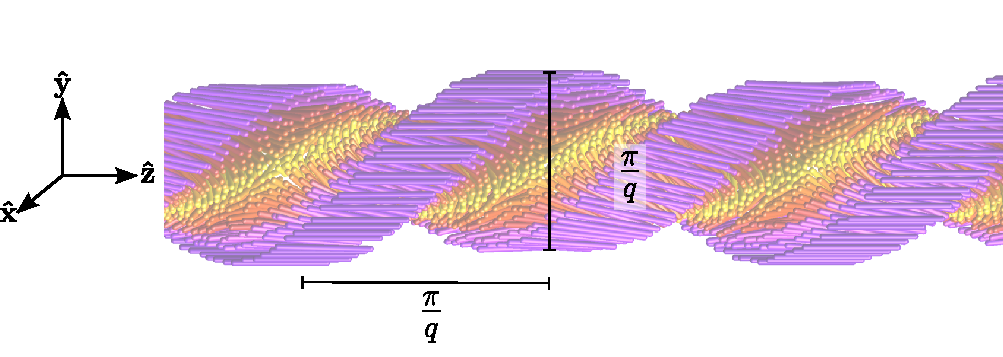
\includegraphics[width= \columnwidth]{figures/chapter-5/ribbon_sketch}.
\caption{ \label{ribsnap} Schematic structure of of twisted ribbon of width $s_y=2\ell$ composed of strongly chiral spherocylinders with aspect ratio $\ell = 15$ mixed with non-adsorbing polymers (not shown) providing strong depletion attraction between the rods. The rods are color coded by orientation. The typical  ribbon dimensions are indicated by the pitch $q$ with $\pi/q$ corresponding to a half pitch length.  }
\end{center}
\end{figure}

At elevated chiral strength the circular membranes are known to transition into twisted ribbons \cite{Gibaud2012}. These were identified as quasi-1D twisted protrusions growing out of the perimeter of the membrane, through a mechanism termed `starfish' instability.


Lowering the temperature strengthens the chiral forces between the rods, which raises the free energy of the interior untwisted rods while lowering the free energy of edge-bound twisted rods. This enables chiral control of edge line tension which, when the edge tension approaches zero,  leads to spontaneously transitions of the membrane into an array of 1D twisted ribbons, called a ‘‘starfish’’ \cite{Gibaud2012}. A phenomenological model aimed at capturing the onset of the surface-driven instability was presented in Ref. \cite{kang_sm2016}. So far, no minimalist theory along the spirit of the one discussed for the membrane has been contemplated for the ribbon whose intricately twisted structure is  depicted in \fig{ribsnap} based on a nematic  director parameterization we are about to present.  While the membrane exhibits double twist in a circularly symmetric fashion, the rods within the ribbon are twisted in two mutually perpendicular directions along the short and long axes of the ribbon.  Then, the director field of a twisted ribbon may be constructed from a combination of two rotation matrices, each corresponding to a twist along mutually perpendicular Cartesian axes. Without loss of generality we fix the director field of the untwisted ribbon along the $x$-axis of the frame $\bn_{0}=(1,0,0)$ so that the director field of the ribbon reads:
\beq
\bn_{r}[ \Phi, \chi] = \mathcal{R}_{xz} [\Phi]\cdot \mathcal{R}_{xy}[\chi] \cdot \bn_{0}
\label{nrib}
\eeq
in terms of the rotation matrices
 \beq
 \mathcal{R}_{xz} [ \Phi]   =
  \begin{bmatrix}
     \cos \Phi(y) & 0 & \sin \Phi(y)  \\
    0 & 1 & 0  \\
    -\sin \Phi(y) &  0 & \cos \Phi(y)  \\
      \end{bmatrix}  \nonumber
      \label{rxz}
 \eeq
and
 \beq
 \mathcal{R}_{xy} [ \chi]   =
  \begin{bmatrix}
     \cos \chi(z) &  \sin \chi(z) & 0  \\
    -\sin \chi(z) &   \cos \chi(z) & 0 \\
      0 & 0 & 1  \\
      \end{bmatrix}  \nonumber
      \label{rxy}
 \eeq
Here, $\Phi$ and $\chi$ denote  two  angles describing the twist along the short and long (ribbon) axes that we parameterize via the coordinates $-s_{y}/2 < y < s_{y}/2$ and $-s_{z}/2< z <s_{z}/2$, respectively. The ribbon area $A = s_{y}s_{z}$ is conserved. We further define the local thickness of the ribbon:
\begin{align}
h = \frac{L}{2}   | \bn_{0} \cdot \bn |  =\frac{L}{2} |\cos \chi(y) \cos \Phi(y)| 
\end{align}
We now simplify matters by assuming linear twist in both directions so that $\chi = qz$ and $\Phi = qy$ where $q$ denotes the principal pitch of the ribbon quantifying the degree of twist along the long and short ribbon axes. We remark that the  ribbon pitch is likely to be different from the value $q_{0}$ that we defined in \eq{qzero} which quantifies the chiral strength between the rods. Henceforth, we will use the ribbon width as our length unit and render all pitches dimensionless via $q \rightarrow q s_{y}$. We assume the ribbon to be long enough so we can ignore surface effects imparted by the short edge of the ribbon. Using the parameterization of the director \eq{nrib} we find that the   contributions corresponding to bend, splay and twist elasticity {\em per unit ribbon length}  reads:
\begin{align}
F_{bend} &=\frac{K_{3}}{16} \left [ 3 q^{2} - q \sin q (\cos q -2)\right ]  \nonumber \\ 
F_{splay} &=  
\frac{K_{1}}{8}  (q^{2}  - q \sin q )  \nonumber \\ 
F_{twist} &=  \frac{K_{2} }{16  }  \left [ 8 q_{0}(q_{0} -q -\sin q)  + q\sin q ( \cos
   q +4) + 7 q^{2}\right ]
\end{align}
Note that the bulk elastic energies   are all {\em even} functions of the pitch $q$, expect the first term in the twist contribution which encodes chirality and vanishes for achiral rods ($q_{0} =0$). 
 We must also consider the effect of saddle-splay, which is nonzero due to the curvature of the ribbon (it does not play a role for the flat membranes). It can be defined in terms of the following bulk contribution to the Frank elastic energy: 
\beq
F_{saddle} = -\frac{K_{24}}{2} \int d \bfr   [\nabla \cdot ( \bn \nabla \cdot \bn +  \bn \times \nabla \times \bn )]
\eeq
which gives:
\beq
F_{saddle} = -\frac{K_{24} }{4 }  q \sin q
\eeq
The depletion contribution \eq{fdep1} can be derived in a similar way. Ignoring factors independent of the pitch, we find:
\begin{align}
F_{dep}  & \sim  2 n_{p} a k_{B}T \left  [  \frac{(qL)^{2}}{16}  + \oint d \ell h \right ] 
\end{align}
Twisting a rectangular slab into a ribbon enhances the contour length of the object, which is reflected in the line integral in \eq{fdep1} that we express as $\oint d {\bf l}h = (q/2 \pi)\sqrt{1+ (q/2)^{2}}\int_{-\pi/q}^{\pi/q} dz h$. With this we find a simple expression:
\beq
 \oint d {\bf l} h  = \frac{2L}{\pi} | \cos  (\tfrac{1}{2} q) |    \sqrt{1+ \tfrac{1}{4} q^{2}} 
\eeq
which suggests  that the  tension contribution is minimal at maximum tilt at the ribbon edge when $q = \pm \pi $. Simultaneously, it penalizes large pitches as the perimeter-to-area ratio of the ribbon increases with the degree of longitudinal twist, although this effect is of minor importance.  


\begin{figure}
\begin{center}
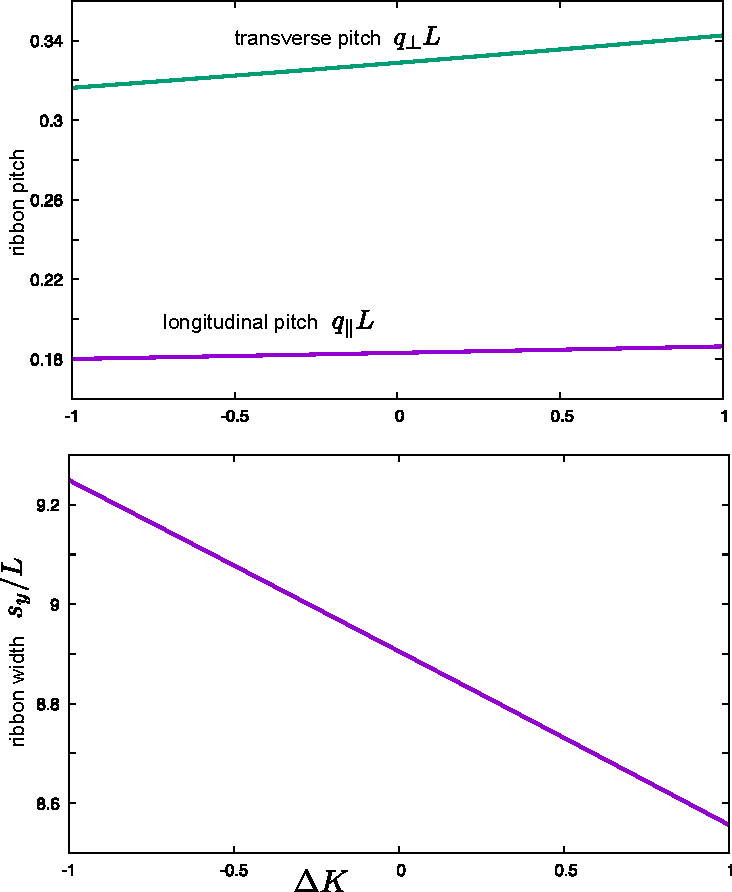
\includegraphics[width=   \columnwidth]{figures/chapter-5/deltak}.
\caption{ \label{ribbontheory} Overview of the ribbon properties as a function of the elastic anisotropy $\Delta K$ [\eq{dk}] of the LC material. Parameters $\lambda_{t} = 0.5 L$ and $q_{0} = 0.4 L^{-1}$. Shown are (a) the longitudinal and transverse ribbon pitches. (b) The equilibrium ribbon width in units rod length $L$. (c) The typical ribbon aspect ratio in terms of the longitudinal pitch versus ribbon width. (d) The tilt angle at the ribbon edge.   }
\end{center}
\end{figure}


Although the expressions obtained are entirely algebraic,  minimization of the total free energy can only be performed numerically. To make progress, we  expand the free energy contributions up to quadratic order in $q$.
Combining terms and reintroducing the twist penetration length $\lambda_{t}$ we arrive at a compact expression for the total free energy per unit length of a weakly twisted ribbon ($q \ll 1/s_{y}$): 
\beq
\frac{F}{K_{2}} \sim   -q q_{0}   +  \frac{1}{2}\left ( \frac{\Delta K}{2} + \frac{L^{2}}{8\lambda_{t}^{2}}\right )  q^{2} + \frac{2 L }{\pi \lambda_{t}^{2}}
\label{flowq}
\eeq
The first two term encodes the free energy change due to (chiral) twist, the second  the effect of splay, bend and saddle-splay elasticity along with depletion, whereas the last term denotes the line tension which up to leading order does not depend on the pitch.  The constant $\Delta K$ represents a combination of the  bend-twist and saddle-twist elastic anisotropies:
\beq
\Delta K = \frac{K_{3}}{K_{2}} - \frac{K_{24}}{K_{2}} + 3
\label{dk}
\eeq
The equilibrium ribbon pitch follows from minimizing \eq{flowq} and is related to $q_{0}$ via:
\begin{align}
q & \sim q_{0} \left ( \frac{\Delta K}{2} + \frac{L^{2}}{8\lambda_{t}^{2}}\right )^{-1}  
\end{align}
Inserting this back into the quadratic free energy and reexpressing all variables in bare units we find:
\beq
\frac{F}{K_{2}} \sim -\frac{1}{2} \left ( \frac{\Delta K}{2} + \frac{L^{2}}{8\lambda_{t}^{2}}\right ) (q_{0} s_{y})^{2} + \frac{2 Ls_{y} }{\pi \lambda_{t}^{2}}
\eeq
which combines a bulk term proportional to $s_{y}^{2}$ and a surface contribution  linear in $s_{y}$. Minimization yield for the typical ribbon width:
\beq
s_{y} \sim \frac{2 L }{ \pi \lambda_{t}^{2} q_{0}^{2} } \left ( \frac{\Delta K}{2} + \frac{L^{2}}{8\lambda_{t}^{2}}\right ) 
\eeq
Finally, we deduce  the ribbon pitch versus width:
\beq
\frac{\textrm{ribbon pitch}}{\textrm{ribbon width}} = \frac{2 \pi}{q s_{y}} \sim  \frac{\pi^{2} q_{0} \lambda_{t}^{2} }{L}
\eeq
and the tilt angle at the ribbon edge:
\beq
\Phi(y = s_{y}/2) = \frac{1}{2} q s_{y} \sim \frac{L}{\pi q_{0} \lambda_{t}^{2}}
\eeq
The predictions above should be qualitatively correct and give valuable insight into how the ribbon properties depend on, for instance, the intrinsic chirality and elasticity of the LC material.  A potential caveat of the low-$q$ expansion, however, is that ribbons form at elevated chirality where the ribbon pitch $qL$ is not necessarily a small parameter ($qL \ll 1$). Because deviations from the simple quadratic free energy \eq{flowq} are to be expected, we chose to minimize the free energy numerically which is an easy task given that all free energy contributions  are in  algebraic form.

In doing so, we may also probe a more general scenario where the twist along the principal ribbon directions is {\em anisotropic}. To this end, we characterize  the twist angles  via $\chi = q_{\parallel} z$ and $\Phi = q_{\perp}y$ in terms of a longitudinal and transverse pitch, $q_{\parallel}$ and $q_{\perp}$, respectively. 
 Typical input values  for the case of {\em fd} rods can be obtained by fixing the twist penetration length $\lambda_{t}  = L/2$ \cite{barry_jpcb2009} and taking a typical (cholesteric) pitch $q_{0} = 0.4L^{-1}$. The elastic anisotropy $\Delta K$ is much harder to specify as it depends quite sensitively on the  saddle-splay modulus $K_{24}$ which is unknown for {\em fd} rods. 
The numerical results are shown in \fig{ribbontheory}. The dependence of the quantities on the elastic anisotropy $\Delta K $ is evident but turns out rather weak, indicating that the predictions should be robust against a wide range of elastic properties of the LC material.   We further observe that the twist is indeed considerably anisotropic with the transverse ribbon pitch being larger than  the longitudinal pitch, while both are {\em smaller} than the typical cholesteric pitch $q_{0}$ that quantifies the chiral strength at the rod level. We further infer that the ribbon width is always a few times the rod length, suggesting that ribbons are indeed very slender quasi-1D  objects. The ribbon pitch-to-width ratio is predicted to be about 3, which is in agreement with experimental observations reported in Ref. \cite{Gibaud2012}. A typical value of 5 was quoted in Kaplan {\em et al.} \cite{kaplan2010theory}  for ribbons of {\em fd} rods mixed with non-adsorbing polymer.   Finally, the edge tilt angle is virtually insensitive to $\Delta K$ and is predicted to be about $84 ^\circ$, confirming that the rods make a near  $\pi/2$-twist at the ribbon edge.

The membrane-ribbon transition   could, in principle, be analyzed by comparing the free energies for both twisted morphologies for a given droplet volume. This however is technically very demanding given that the circular symmetry of the membrane, as encoded in the strongly non-linear elastic free energy \eq{fmem},  precludes a tractable analytical solution of the twist angle unlike for the ribbon. Below, we resort to a hand-waving argument as to why a membrane-ribbon transition should or should not take place. 
 
\section{Membrane or ribbon ? }

Having established a minimal theoretical description for the membranes and  ribbons we now wish to explore under which conditions the various droplet morphologies are favored. It is instructive to consider the main energetic effects involved in shaping the droplets, namely a surface energy and a (bulk) chiral energy that is contained in the twisting of the rods within the droplet. The preference for one state or the other can be argued as resulting from a trade-off between these two energies. On the one hand, for any finite membrane volume (or area) flat circular membranes have a minimal surface free energy but are able to accommodate only a limited amount of twist as the result of twist being expelled from the core and confined into a narrow zone of length $\lambda_{t}$ near the membrane edges. Twisted ribbons, in view of their elongated shape, have an unfavorable perimeter-to-area ratio but are much more efficient at accommodating chirality because the twist is {\em uniform} throughout the main section of the object. Using these arguments, a membrane-to-ribbon transition can  be understood as a natural consequence of a controlled experiment in which enforced chirality driven by cooling the system (a mixture of {\em fd} rods with dextran) was found to lead to a simultaneous reduction of the line tension of the membrane \cite{Gibaud2012}.

We now propose a  heuristic argument for the stability of the membrane  by balancing the bulk chiral and interfacial energetic contributions. First, the chiral free energy contained in the twisted rim of the membrane can be estimated from: 
\beq
\frac{F_{\rm chiral}}{K_{2}} \sim 2 \pi \int_{R_{m} - \lambda_{t}}^{R_{m}} d R R \left [ (\partial_{R} \varphi(R))^{2} + q_{0} \partial_{R} \varphi (R) \right ] 
\eeq
ignoring the depletion and curvature contributions for large membranes ($R_{m} \rightarrow \infty $).  Minimization of the free energy yields an analytical solution for the twist angle versus radius, namely $\varphi(R) = -\frac{q_{0}}{2}R + C_{1} \ln R + C_{2}$. The constants $C_{1}$ and $C_{2}$ can be specified from the following boundary conditions:
\begin{align}
\varphi(R_{m} - \lambda_{t}) &= 0 \nonumber \\ 
\lambda_{t} ^{2}\partial_{R} \varphi(R_{m}) &= \frac{L}{2} \sin \varphi(R_{m}) 
\label{bc}
\end{align}
The first refers to the untwisted core at $R < R_{m} - \lambda_{t}$ while the second follows from the interfacial tension at the membrane edge at $R = R_{m}$.  To simplify matters further we fix the twist penetration length at half the rod length $\lambda_{t} =L/2$ \cite{barry_jpcb2009} and linearize the boundary condition via $ \sin \varphi(R_{m})  \approx \varphi(R_{m}) $. The chiral free energy stored in the membrane rim then reads: 
\beq
\frac{F_{\rm  chiral}}{K_{2}} \sim \frac{\pi}{16} (q_{0}L)^{2} \left ( 1 - \frac{4 R_{m}}{L} \right ) 
\eeq
which is negative for large membranes. This free energy must be balanced against the interfacial contribution which in our minimalist approach reads:
\beq
\frac{F_{\rm  interface}}{K_{2}} \sim \frac{4 \pi R_{m}}{L} \cos \varphi(R_{m})
\eeq
with the edge tilt angle being proportional to the chiral strength via $\varphi(R_{m}) = q_{0}/4$. Equating the two expressions and taking an infinitely large membrane $R_{m} \rightarrow \infty$ we find a critical pitch of $q_{0}^{\ast} L = 3.296$.  This means that below this value the interfacial energy outweighs the gain in chiral energy ($F_{\rm interface} + F_{\rm chiral} >0$) and the membrane is stable. At strong chirality, $q_{0} > q_{0}^{\ast}$ the rim contribution dominates and transitions towards elongated twisted structures such as the ribbon can be expected.  The critical pitch increases for finite-sized membranes given that smaller membranes have a relatively larger rim to surface proportion. The membrane-ribbon transition line based on the non-linearized boundary condition \eq{bc} is easily obtained numerically and is given by the purple curve in \fig{emergent}.  We remark that quantitative predictions from the current expressions have to be taken with care because of our simplistic description of the membrane surface tension which does not account for the effect of chirality and does not include curvature corrections that will play a more prominent for small droplets \cite{malijevsky2012perspective}.  A more general expression for the surface tension $\sigma$ of the droplet should therefore read:
\beq
\sigma(R_{m}) \sim 2 n_{p} a k_{B}T \left ( 1 - \frac{2\delta}{R_{m}} \right ) + \sigma_{\rm chiral}  
\eeq
in terms of the Tolman length $\delta$, which could be positive or negative, and a chirality-dependent correction as conjectured in Ref. \cite{Gibaud2012} for the case of {\em fd}. However, both contributions are unknown for our particular simulation model. It is probable that the chirality contribution is very distinct from the one proposed for the experimental case such that the surface tension is little sensitive or even  decreases with  chirality.  Also, the Tolman length could be negative resulting in $\sigma$ rising  for smaller membrane radii \cite{lei2005tolman,malijevsky2012perspective}.   We may therefore assert that the  small membranes simulated in our study are likely to experience a considerable surface tension that constrains the droplets to remain more or less circular. An alternative strategy to cope with high levels of chirality is then to increase the perimeter of twisted zones at the interior of the membranes by splitting into multiple cores with shared interfaces, reminiscent of domains walls.  Within the interfacial zones between the cores the rods display a $\pi/2$ twist from the local core (see \fig{multidomain}). This enables adjacent cores to share an interface with no incommensurability in the edge twist. The interfacial cost imparted by  the domain walls is likely to be much smaller than that of the membrane and its surrounding polymer fluid.  


\begin{figure}
\begin{center}
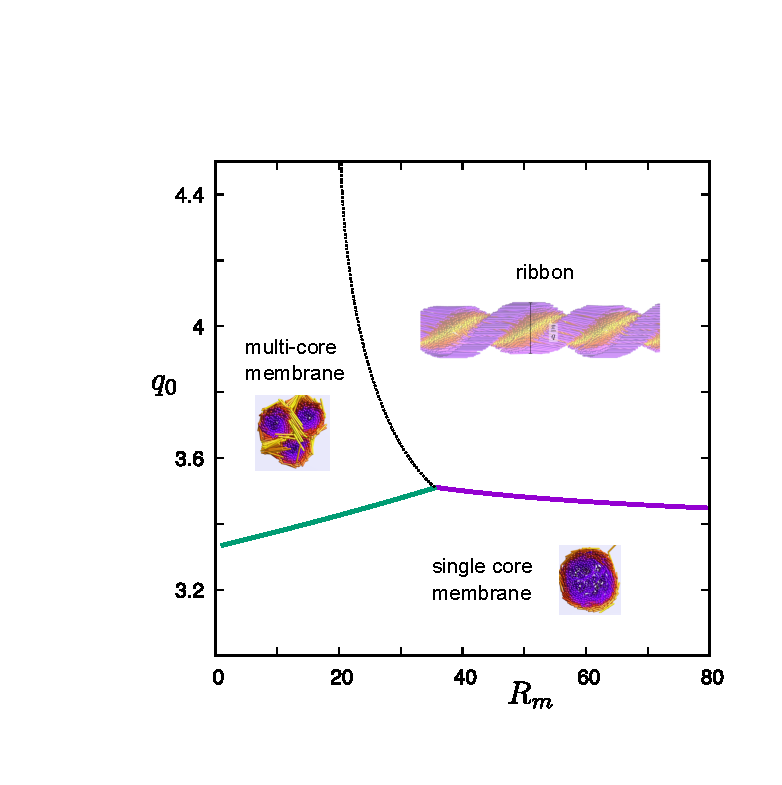
\includegraphics[width=  0.8 \columnwidth]{figures/chapter-5/emergent}.
\caption{ \label{emergent} Overview of the various membrane morphologies predicted for chiral colloidal rods mixed with non-adsorbing polymer as a function of the membrane radius $R_{m}$  and pitch $q_{0}$ (both expressed in units of the rod length $L$). Depending on the membrane radius,  weakly chiral rods tend to self-assemble into single-core twisted membranes but may transition into elongated twisted ribbons beyond a critical chiral strength. Small droplets tend to be curbed by surface tension and are precluded from forming ribbons,  developing into multi-core membranes instead (see also \fig{multidomain}).   }
\end{center}
\end{figure}


 A naive estimate of the transition from the single to a multi-core membrane can be established by comparing the chiral energy of the two states. Let us focus on the simplest case, namely the one composed of three cores [\fig{multidomain}(b) for $\varepsilon_{c}=12$] and denote the radius of each core by $R_{s} = R_{m}/\sqrt{3}$ which guarantees conservation of the total membrane area. Furthermore, we assume that the twist angle at the subcore edge is $\pi/2$ so that the second boundary condition in \eq{bc} should be replaced by $\varphi(R_{s}) = \pi/2 $. Then, the chiral energy contained in each subcore rim reads:
 \beq
 \frac{F_{\rm  chiral}^{(s)}}{K_{2}}  \sim \frac{\pi}{4} q_{0}^{2} \left ( \lambda_{t}^{2} - 2 \lambda_{t} R_{s} \right ) + 2(\pi + \lambda_{t} q_{0} )^{2} \ln \left ( \frac{R_{s} - \lambda_{t}}{R_{s}} \right ) 
 \eeq
Balancing this against the single-core free energy $F_{\rm chiral} = 3 F_{\rm chiral}^{(s)}$ and assuming the interfacial contribution to be the same for both states we find a simple criterion for the onset of multi-domain order. The result is given by the green curve in \fig{emergent}.  In our simulations, we find the single-to-triple core transition to occur around $\varepsilon_{c} =12$.  According to \eq{qzero} for $\rho_{0} \sim 0.5D^{-2}$ this  corresponds to about $q_{0} \approx 0.9$ which is considerably smaller than the value predicted from our naive free energy balance. Combined with the prediction for the (single core) membrane-ribbon transition we construct a tentative state diagram stipulating the conditions for the different morphologies as shown in \fig{emergent}. We speculate that the multi-domain structures, in view of their enhanced capacity to harbour strong twists,  retain their morphology and do not transition into ribbons even at elevated chiral strength. This is tentatively indicates by the dotted black curve. The key conclusion to be drawn  from the diagram is that ribbons are more likely to appear from large membranes (say $R_{m}  > 50 L$) than from small ones. Taking a typical membrane density of $0.5 D^{-2}$ [cf. \fig{density}] we find that the required system size far exceeds the ones probed in our study,  $N > 25 \pi (L/D)^{2} \sim 8000$ for $L/D = 10$.  This clearly poses a significant challenge for future simulation efforts that should be directed towards modelling rod-polymer mixtures using high-performance Molecular Dynamics computations capable of handling system sizes of about an order of magnitude larger than ours. 






%where  $q \ll q_{0}$ depending on the elastic anisotropy and twist penetration length. We remark that the ribbon pitch does not depend on the line tension (second term in \eq{flowq} which is independent of $q$).  

% Check minimize free energy per pitch versus per unit length = 2pi/qq. Combined minimization wrt qq and sy by reverting free energy to bare units rod length.



%Before proceeding with our analysis we immediately infer a couple of basic facts from inspecting \eq{fribbon}. First, as expected chiral forces between the rods, represented by the term proportional to $2-\tau^{2}$, lower the free energy provided the ribbons are sufficiently elongated ($\tau  >\sqrt{2})$. A further stabilization mechanism occurs through the line tension since the curvature correction $w_{2}$ is negative. 

%The relevant constants $\Delta K$ and $\Delta \ell$ can be estimated from the twist penetration length. Taking the reference value $\lambda_{t} = L/2$ quoted for {\em fd} virus rods we find that  $\Delta K \sim (L/2\lambda_{t})^{2} \sim 1 $,  ignoring weak contributions from the bend-to-twist and saddle-splay elasticity. Similarly, we obtain $\Delta \ell \approx 4 $ for a ribbon with a lateral width equal to the rod length $s_{y} = L$. For the pitch we roughly estimate $q_{0} = 2 \pi s_{y} / p_{c} \approx 0.2$ taking a cholesteric pitch  $p_{c} \sim 30L$. 

%The next step is to minimize the free energy \eq{fribbon} with respect to the ribbon pitch $q$ and aspect ratio $\tau$, i.e., $\partial F/\partial q =0$ and $\partial F/\partial \tau =0$ for a given ribbon area $A$. If the line tension is ignored ($\Delta \ell =0$), the extremum condition can be solved analytically and gives an equilibrium ribbon pitch:
%\beq
%q =  \frac{3q_{0}}{4 \Delta K} \frac{(\tau^{2} -2)}{1 + \tau^{2}}
%\eeq
%where the last contribution is a monotonically increasing function for $\tau^{2} >2$ levelling off to unity for $\tau \gg 1$. The ribbon free energy per unit area corresponding to the optimal pitch is:
%\beq
%\frac{F/\tau}{K_{2}}  = -\frac{1}{96} q_{0}  (\tau^{2} -2) q^{3}
%\eeq
%From this we infer that (i) stable ribbons that are not curbed by line tension penalty tend to stretch to very large aspect ratios, and (ii) the limiting pitch at large ribbon aspect ratio is likely smaller than the membrane pitch $q_{0}$ given that $q =  3q_{0}/4 \Delta K$ for $\tau \rightarrow \infty $ and $\Delta K \sim 1$. In practice, conservation of area precludes the ribbons to stretch to infinity while a finite line tension puts a further natural bound to $\tau$. 



%\subsection{Effect of anisotropic twist} 

%\begin{figure}
%\begin{center}
%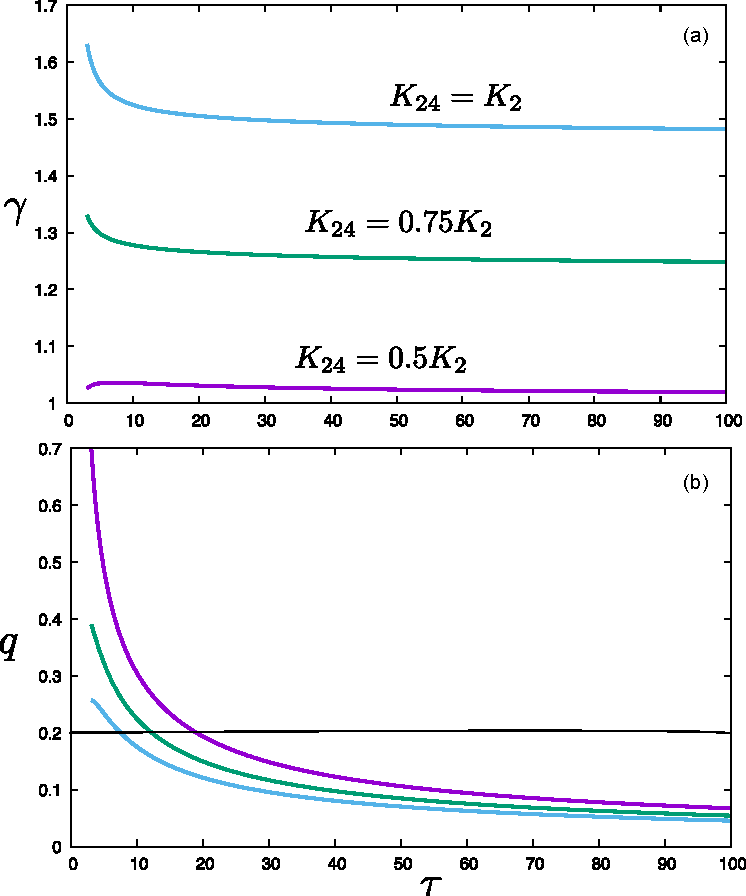
\includegraphics[width=  0.5 \columnwidth]{figures/chapter-5/raniso}.
%\caption{ \label{fig3} Twist anisotropy $\gamma$ and pitch $q$ of a twisted ribbon with width $s_{y} = L$ as a function of the %ribbon length $\tau$. The chiral strength between the rods is given by the membrane pitch $q_{0} = 0.2L^{-1}$ (horizontal black %line). The twist penetration length is $\lambda_{t} = 0.5L $.   }
%\end{center}
%\end{figure}


%Let us now explore the possibility of unequal twist along the short and long ribbon axes. This should render a more realistic picture of the internal twist profile of the ribbon  given that the twist along the principal ribbon directions need not have the same magnitude. We proceed by allowing $\gamma$, which denotes the ratio between the degree of twist along the long and short axes  of the ribbon,  to be a  variable quantity. Working out the algebraic free energy per area we find for the bulk elastic contribution:
%\begin{align}
%\frac{F}{ K_{2} \tau} &\sim 
%\frac{1}{24} \left [ \frac{K_{3}}{K_{2}} q^{4} (1 + \tau^{2}) \gamma^{2} + B\right ]
%\end{align}
%with $B$ the twist elastic contribution:
%\beq
%B = (q_{0} + q - q \gamma) (12 q_{0} + q (12 - \gamma (12 + q^2 ( \tau^{2} \gamma -2))))
%\eeq
%This term reduces to the much simpler expression explored in the previous section for the isotropic twist case ($\gamma =1$). Similarly, the saddle-splay term now becomes:
%\beq
% \frac{F}{K_{2} \tau} \sim  - \frac{1}{24}\frac{K_{24}}{ K_{2} } q^{4} \gamma (1 + \tau^{2} \gamma)
%\eeq
%Finally the depletion free energy reads (ignoring irrelevant constants as well as the line tension contribution):
%\beq
% \frac{F}{K_{2} \tau} \sim  \frac{L^{2}}{96 \lambda_{t}^{2}} q^{4} (1 + \tau^{2} \gamma^{4})
%\eeq
%Clearly, these complex expressions are no longer amenable to further analytical treatment. Furthermore, the elastic and depletion strengths can longer be compactly combined into a  single parameter $\eq{dk}$ as could be done for the isotropic twist case but must be  separately defined. However, minimization of the three free energy terms above with respect to $q$ and $\gamma$ is easily carried out numerically and the results are shown in \fig{fig3} taking $K_{3}/K_{2} = 1/4$, $q_{0} = 0.2$, $\lambda_{t} = L/2$ and three different values for the saddle-splay elastic modulus. Clearly,  $\gamma $ tends to be larger than unity depending on the strength of the saddle-splay elasticity $K_{24}$ indicating twisting along the main ribbon axis can be about 30-50 \% stronger than across the short axis. We remark that $K_{24}$ plays an essential role in driving the  twist for the ribbon geometry. In fact, saddle-splay elasticity cannot be ignored given that  no physical solutions of the minimization problem were found  for $K_{24} =0$. The lowest value explored ($K_{24} = K_{2}/2$) roughly recovers the previous scenario of equal twist along the short and long ribbon axes. The fact that a positive value of the $K_{24}$ is required for stabilizing ribbons is consistent with the work of Kaplan {\rm et al.} \cite{kaplan2010theory} providing a more wide-ranging theoretical framework for membranes and ribbons  based on a Helfrich-DeGennes model which also considers the effect of layer bending (ignored in our model).  

%We further conclude from \fig{fig3}b that longer ribbons tend to be less twisted than short ones.   Short ribbons ($\tau <10$) seem {\em overtwisted} compared to that of the equivalent (single twist) cholesteric phase while long ribbons experience less twist. In all cases we see that $q$ levels off to a limiting value $q < q_{0}$ for infinitely stretched ribbons ($\tau \rightarrow \infty$) in line with our analytical predictions for the case of constrained isotropic twist $\gamma =1$. The line tension, ignored in the results of \fig{fig3}, will put a constraint on the optimal aspect ratio $\tau$ which needs to optimized along with $q$ and $\gamma$ for a given ribbon area. We will not pursue this further in this study given that, in experiment, the line tension at the starfish transition is very low while the available virus material and hence the area tends to be quite large. Both  factors enable these ribbons to grow into strongly elongated objects. This should be compared to our predictions for the limiting case $\tau \rightarrow \infty$. Further restriction  to applying our model to experiments relates to the unknown saddle-splay constant for {\em fd} virus rods. 

%A further characteristic we may deduce from our model is the typical long-axis pitch, in the experiments simply referred to as the pitch,  versus ribbon width.  This ratio of length scales is given by:
%\beq
%\frac{\textrm{ribbon   pitch}}{\textrm{ribbon width}} \sim \frac{2 \pi}{\gamma q s_{y}} 
%\eeq
%From the optical microscopy pictures provided in Ref.  \cite{Gibaud2012} we roughly infer that this ratio should be about 2-3. Taking ribbons of moderate length, say  $\tau = 5$, we find that the predicted ratio is somewhat larger ($\sim 10$), in qualitative agreement with experimental observation.




\section{Conclusions}

%Inspired by recent experimental observations of nmorphological transition of LC membranes colloidal rods mixed with non-adsorbing polymers we have embarked on   Using large scale Monte Carlo simulations combined with liquid crystal continuum theory based onthe Frank elasticity  we have explored mesoscale droplet of colloirdal rods mixed with non-adsorbing polymer



\clearpage








 % Cholesterics: collective effects

\chapter{Morphology of strongly confined tactoids of colloidal rods stabilized by \\
polymer depletion}
\chaptermark{Morphology of strongly confined tactoids}

\section{Background}

Elongated colloids such as, for example,  filamentous {\em fd} rods, mixed with non-adsorbing polymer form compact tactoids due to the strong depletion attractions experienced by the rods. The size and concentration of the polymer can be exploited to  tune the morphology and internal structure of the droplets. Further complexity can be achieved by the presence of strong geometric confinement.  In our study we consider a slab geometry with width comparable to the rod length. The confinement is expected to generate tactoids with a strongly non-uniform rod density whose morphology is further controlled by strong electrostatic and chiral twist between the individual rods as well as by a surface tension that strongly depends on the average rod orientation with respect to the surface normal. In fact, the presence of the wall imparts a wall-liquid surface tension which is likely to be different from the liquid-gas surface tension which would dominate in the bulk case.

We study these systems by means of Monte Carlo simulations in the semi-grand canonical ensemble ($N,V,\mu_{p},T$) consisting of a system of $N$ rods in a volume $V$ at constant temperature $T$ in osmotic equilibrium with a polymer reservoir at constant chemical potential $\mu_{p}$. The number of polymers  $N_{p}$ in the system is then a fluctuating quantity with the average polymer concentration controlled by $\mu_{p}$.

\section{Model}

We consider a system of $N$ rigid spherocylinders of length $L$, thickness $D$ and aspect ratio $L/D= 10$. The spherocylinders are a simplified representation of {\em fd} rods that are much thinner ($L/D > 100$) and carry a small degree of backbone flexibility with persistence length $\ell_{p} \gg L$. Since the large particle aspect ratio in combination with backbone flexibility poses considerable limitations on the numerical efficiency of our simulations  we  only consider rigid rods with a relatively short length assuming that the key features of the confined tactoids do not  critically depend on the rod aspect ratio or flexibility.

The spherocylinders are mixed with non-adsorbing polymers that in our model act as non-penetrable hard spheres with diameter $\sigma$ equalling once or twice that of the spherocylinder ($\sigma = D$ or $2D$). Polymer-polymer interactions are zero, while the interaction between a polymer and a spherocylinder are treated as being strictly hard;  the potential energy is infinitely large when a  sphere and spherocylinder overlap and zero otherwise.



\begin{figure}
	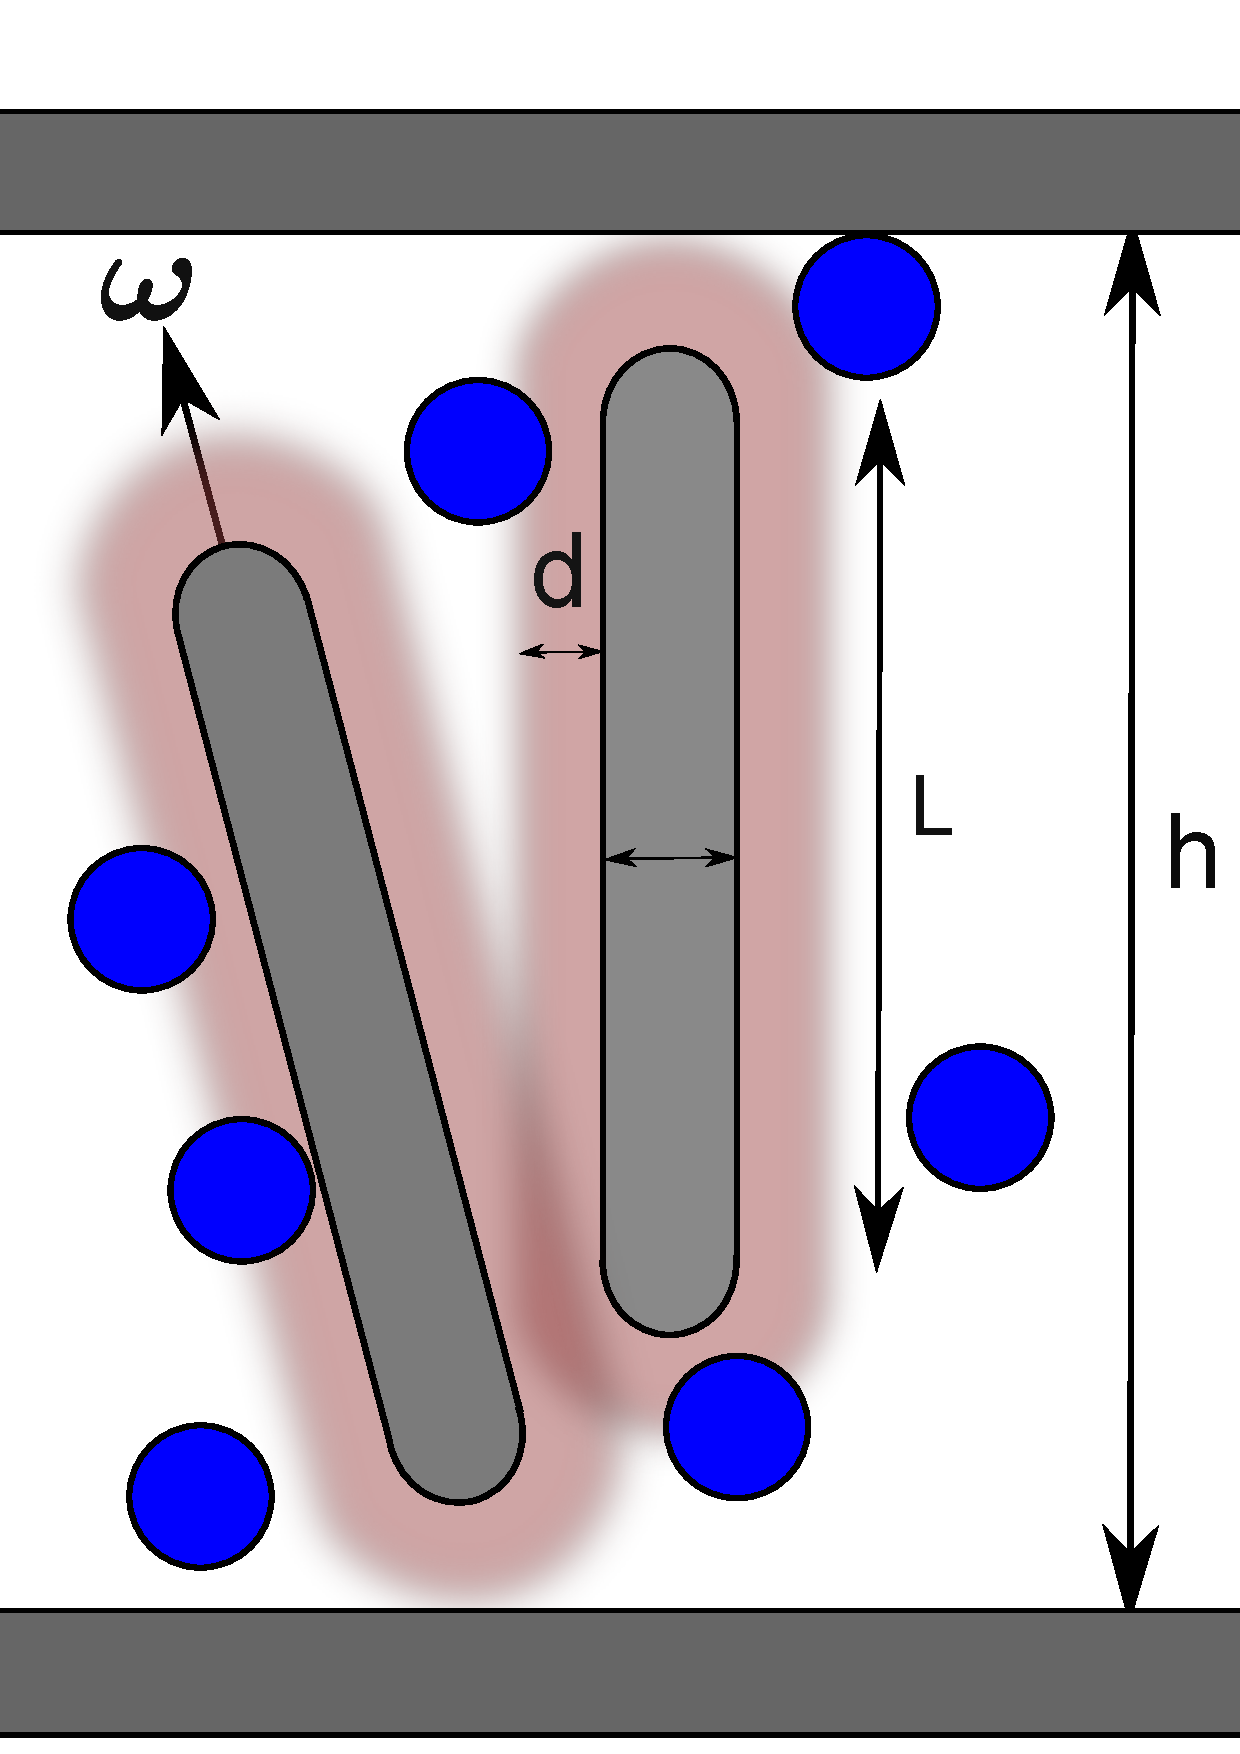
\includegraphics[width = 0.5 \columnwidth]{figures/chapter-6/spheromans}
	\caption{ Sketch of the simulation model: hard spherocylinders (grey) mixed non-penetrable polymers (blue) with diameter $\sigma = D$ (as depicted here) confined in a slab geometry with wall-to-wall distance $h$. Overlap of the cores (grey) gives infinite repulsion while overlapping coronae (blurred zones) favors a twisted pair configuration representing the (chiral) electrostatic forces between {\em fd} rods. Note that our model is defined in three spatial dimensions. }
	\label{sketch}
\end{figure}



The pair interaction $U_{r}$ between two spherocylinders with solid angles $\oma$ and $\omb$ and centre-of-mass distance $\Delta \bfr$ follows from a combination of short-range steric forces (treated as strictly hard) and electrostatic forces at larger distance. The  interaction potential between a pair rods depends on centre-of-mass distance vector $\Delta {\bf r}$ and orientation vector $\oma$ of both rods. In our model, the interactions are encapsulated in the following core-shell potential:
\beq
U_{\rm r} (\Delta {\bf r}, \oma, \omb) =
\begin{cases}
\infty & \textrm{if hard cores overlap}\\
U_{\rm twist} & \textrm{otherwise} \\
\end{cases}
\label{urod}
\eeq
The electrostatic interactions between {\em fd} rods gives rise to so-called electrostatic twist which is intimately linked to the chirality surface architecture of {\em fd} virus rods. The chiral  potential is commonly expressed in terms of a pseudoscalar form initially put forward by Goossens:
\beq
U_{\rm twist} (\Delta {\bf r}, \oma , \omb )=
-\varepsilon_{c} \left ( \frac{D}{\Delta r} \right )^{7}(\oma \cdot \omb)(\oma \times \omb \cdot \Delta \hat{\bf r})
\eeq
where  $\Delta \hat{\bf r} $ denotes a unit vector for the centre-of-mass distance.
 The sign of $\varepsilon_{c}$ defines the microscopic handedness of the rods. Without loss of generality we take $\varepsilon_{c} > 0$ reflecting the right-handedness of {\em fd} rods. The chiral symmetry of the potential is expressed by the pseudoscalar that imparts a sign change upon  inversion $\Delta \hat{\bf r} \rightarrow - \Delta \hat{\bf r}$. In view of its rapid decay with $\Delta r$ the potential is very short-ranged and the rods need to be very close together in order to feel the chiral twist.

 %For simplicity, we assume that the twisting forces are sufficiently short-ranged (which should be the case at sufficient ionic strength) and do not  continuously vary with the centre-of-mass distance between the spherocylinders, but are only operative if the coronae between the rods overlap (see \fig{sketch}).


 The typical attraction energy between two rods due to polymer depletion can be estimated from free-volume theory \cite{lekkerkerker2011depletion} and reads:
 \beq
 U_{\rm r,dep} \sim -\Pi_{P} V_{\rm r, ov}
 \eeq
with $ \Pi_{P} = k_{B} T N_{P}/V$ the (van 't Hoff) osmotic pressure of the polymer reservoir and $V_{\rm r, ov}$ the overlap volume  of the depletion layers surrounding each rod which depends on the orientation of each rod. In case the rods are perfectly parallel and at hard-core contact we find a simple analytical result. Ignoring  finite rod size effects we have:
\beq
V_{\rm r, ov} = LD^{2} \left [  2 r^{2} \cos^{-1} \left ( \tfrac{1}{2r} \right )  - \tfrac{1}{2} \sqrt{4 r^{2} -1}  \right ]
\eeq
with $r = \tfrac{1}{2}(1 + \tfrac{\sigma}{D})$. Rescaling in terms of the polymer packing fraction in the reservoir we find that the maximum depletion strength per rod pair  reads:
\beq
  U_{\rm r,dep} \sim - k_{B}T \phi_{P}  \frac{L}{D} \left ( \frac{D}{\sigma} \right )^{3} \left [  2 r^{2} \cos^{-1} \left ( \tfrac{1}{2r} \right )  - \tfrac{1}{2} \sqrt{4 r^{2} -1} \right ]
 \eeq
For a typical set-up ($\phi_{P} =3$, $\sigma = 2D$ and $L/D=10$) this gives about 15 $k_{B}T$ \red{Please verify this}. It is important to keep in mind that the typical energy due to chiral twist should be small ($ | \varepsilon_{c} | \ll U_{\rm r,dep} $) in order to ensure that the cohesive forces among the rods residing in a droplet are dominated by polymer depletion, with chiral twist playing only a perturbative role.


The rods and polymers are confined in a thin slab of width $h = L$ (see \fig{sketch}). The wall-spherocylinder interactions  are strictly hard, that is, infinite repulsion when the spherocylinder core overlaps with the wall and zero repulsion otherwise. More specifically:
\beq
U_{\rm w} (\Delta {\bf r}, \oma) =
\begin{cases}
\infty &  | \Delta {\bf r} \cdot {\bf \hat{n}} | < \frac{L}{2}  | \oma \cdot {\bf \hat{n}} | + \tfrac{D}{2} \\
\infty &   h-  | \Delta {\bf r} \cdot {\bf \hat{n}} | < \frac{L}{2}  | \oma \cdot {\bf \hat{n}} | + \tfrac{D}{2} \\
0 & \textrm{otherwise}
\end{cases}
\label{urodwall}
\eeq
with ${\bf \hat{n} }$ denoting the wall normal.
The polymers do not have any interaction with the wall, but their centres-of-mass are constrained  to reside within the slab.

The simulations are carried out in the semi-grand ensemble, with a fixed number of rods but the polymer content in the system fluctuating against a virtual reservoir consisting of an ideal gas of polymer spheres with a prescribed chemical potential  $\mu_{p}$ which is trivially connected to the polymer packing fraction via:
\beq
\phi_{P} = \frac{\pi D^{3}}{ 6 \Lambda_{p}^{3} } e^{\beta \mu_{P}}
\eeq
where $\Lambda_{P}$ denotes the thermal (de Broglie) wavelength.


Each MC cycle consists of $N + N_{P}$ randomly chosen rod translations, rotations, polymer insertions or removals. The step size for the spherocylinder translations and rotations are chosen adaptively such as to maintain an average acceptance ratio of about 30 \%. The MC code is optimized using cell-linked list routines that significantly reduce the number of overlap checks between rod-rod and rod-polymer pairs involved in  each MC step. \red{Here we need to specify Glaser's cluster move optimization algorithm that we used \cite{glaser2015parallel}.}  We keep a rectangular box shape with $L_{x} = L_{y}$ and $L_{z} = L$ and periodic boundary conditions (PBC) in both lateral directions.

Besides the planar confinement $h$, a further key parameter is the relative strength of chiral twist versus depletion attraction. These can be combined into a dimensionless parameter $\chi_{T}$ balancing the energy scales associated with twist and depletion as previously discussed:
\beq
\chi_{T} = \frac{\varepsilon_{c}}{U_{\rm r, dep}} \ll 1
\eeq
so that twist becomes more prevalent for larger $\chi_{T}$.

Depending on the polymer size the system will either evolve into a liquid drop ("tactoid") or  will retain its crystalline inner structure (expected for `sticky' depletion forces induced by small polymers, $\sigma = D$). We monitor the {\em system} polymer concentration and total twist energy $\mathcal{U}  = \sum_{i}\sum_{j<i}U_{\rm twist}$ to gauge whether or not the drop has reached its equilibrium state.

We plan to focus on two different systems:

\begin{itemize}
\item  i) Small polymers with $\sigma = D$ imparting short-ranged attractions. The initial configuration is a square monolayer of perfectly parallel rods ordered into a hexagonal lattice. Without confinement, the cluster will equilibrate into a membrane with  fluid order. In. our simulations we fix the polymer concentrations $\phi_{P}=1$ and $N=2000$. Note that small changes in $\epsilon_{c}$ may have large consequences for the way the droplet expresses chiral twist. At weak twist ($\varepsilon_{c} < ****$), the membrane remains circular in shape with twist showing up at the membrane edges while the membrane center remains largely unperturbed. At strong twist ($\varepsilon > ****$) the membrane may transform into a twisted ribbon. \red{The first indication of such a change of droplet morphology can be observed in \fig{samples} a and c.   Bigger systems ($N=2000$) spontaneously form ribbon-shaped protrusions around a circular central body which resembles the onset of twisted ribbon formation.  }.  Next we introduce confinement and re-assess the droplet shape and internal structure and compare with experimental observations.

\item ii) Large polymers with $\sigma = 2 D$ imparting long-ranged attractions. We start from the same monolayer crystal which will equilibrate into a liquid tactoid in bulk \cite{kuhnhold2022structure}. Gradually increasing the confinement (at $R_{2} > h$ with $R_{2}$ the minor curvature radius of an unconfined tactoid \cite{kuhnhold2022structure})  will lead to squeezed tactoids which  develop a distinct biaxial shape. Introducing twist may lead to further morphological changes. We may correlate droplet size ($N$) with droplet aspect ratio for the strongly confined case compared to the 3D case studied in \cite{kuhnhold2022structure}.

\end{itemize}


\section{Glaser's Algorithm}

\section{Results}

\begin{figure}
	\includegraphics[width = .7\columnwidth]{figures/chapter-6/samples}
	\caption{Membrane-shaped tactoids of chiral rods mixed with non-adsorbing polymer formed in bulk (no confinement). For all runs, $\sigma = D$, chiral radius $d = 0.4D$, $\phi_{P}$ and $N = 500$. (a)-(b) $\varepsilon_{c}=0.5k_BT$, (c)-(d) $\varepsilon_{c}=1k_BT$ Top panels (a),(c) correspond to a top view of the system, bottom panels (b), (d) correspond to a side view with angle indicated by an arrow at the top panels.}
	\label{samples}
\end{figure}

\begin{figure}
	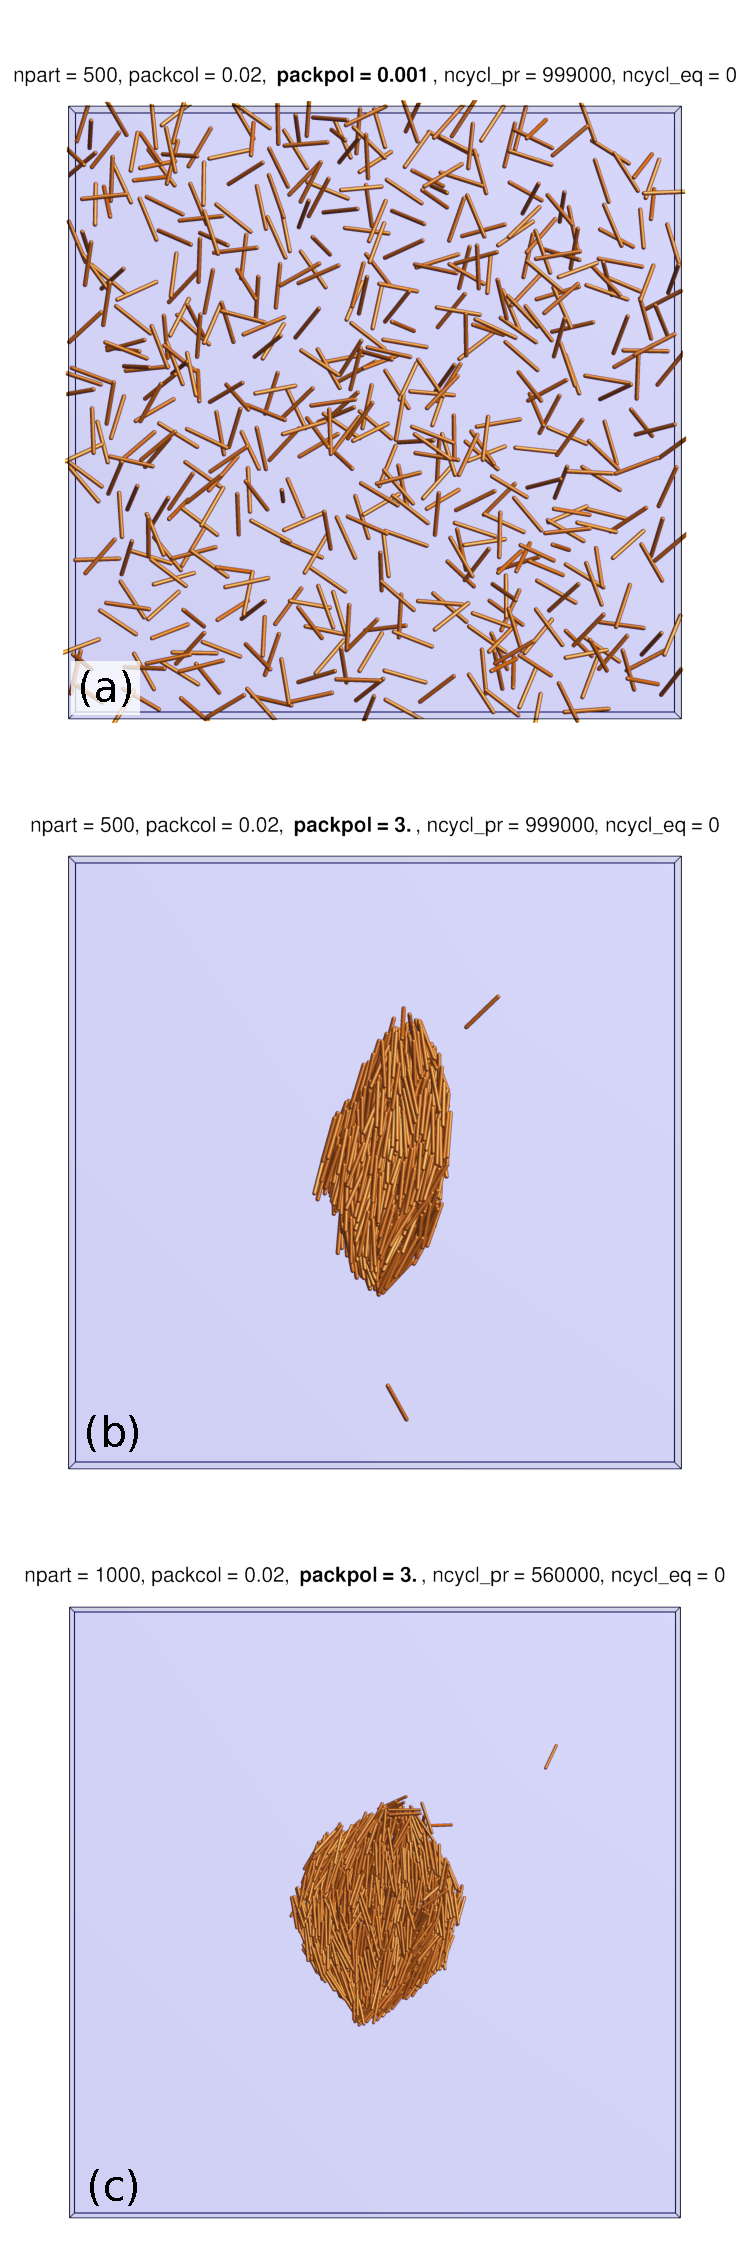
\includegraphics[width = 0.4 \columnwidth]{figures/chapter-6/impl_depletion_effect}
	\caption{ Spindle-shaped tactoids of achiral rods ($\varepsilon_{c}=0$) mixed with non-adsorbing polymer ($\sigma = 2D$) \red{in strong planar confinement ($h = L+D$)}. a) Weak depletion  (very low polymer packing fraction) and $N=500$. b) Strong depletion; $\phi_{P} =3$, $N=500$. c) Strong depletion; $\phi_{P} =3$, $N=1000$. The difference between the shapes between (b) and (c) is explained in \cite{kuhnhold2022structure} for 3-dimensional tactoids: larger nematic droplets tend to be less elongated. The structure in panel (b) is used as an initial configuration in the samples shown in \fig{samples}}
	\label{notwist}
\end{figure}



\clearpage % Nematic droplets

\chapter{Conclusions}

\red{Text from template, to be filled.}

%%%%%%%%%%%%%%%%%%%%%%%%%%%%%%%%%%%%%%%%%%%%%%%%%%%
%                  1. Figure
%%%%%%%%%%%%%%%%%%%%%%%%%%%%%%%%%%%%%%%%%%%%%%%%%%%

\section{Figure}

You can use tikz package to plot like figure ~\ref{fig:arch_comp}.

\begin{figure}[!htb]
    \centering
    \begin{subfigure}[b]{0.45\textwidth}
        \centering
        \begin{tikzpicture}
        \node[input] (mi) {};
        \node[block,right=of mi] (a) {$\mathrm{E}\left(p_k, \cdot\right)$};
        \node[block,right=of a] (b) {$\mathrm{D}\left(s_k, \cdot\right)$};
        \node[input,below=of a] (pk) {};
        \node[input,below=of b] (sk) {};
        \node[output, right=of b] (mo) {};
        \draw[draw,->] (mi) -- node[above] {$m$} (a);
        \draw[draw,->] (pk) -- node[left] {$p_k$} (a);
        \draw[draw,->] (a) -- node[above] {$c$} (b);
        \draw[draw,->] (sk) -- node[left] {$s_k$} (b);
        \draw[draw,->] (b) -- node[above] {$m$} (mo);
        \end{tikzpicture}
        \caption{Public-Key Architecture}
        \label{fig:pkcs_arch}
    \end{subfigure}
    \begin{subfigure}[b]{0.45\textwidth}
        \centering
        \begin{tikzpicture}
        \node[input] (mi) {};
        \node[block,right=of mi] (a) {$\mathrm{E}\left(k, \cdot\right)$};
        \node[block,right=of a] (b) {$\mathrm{D}\left(k, \cdot\right)$};
        \node[input,below=of a] (pk) {};
        \node[input,below=of b] (sk) {};
        \node[output, right=of b] (mo) {};
        \draw[draw,->] (mi) -- node[above] {$m$} (a);
        \draw[draw,->] (pk) -- node[left] {$k$} (a);
        \draw[draw,->] (a) -- node[above] {$c$} (b);
        \draw[draw,->] (sk) -- node[left] {$k$} (b);
        \draw[draw,->] (b) -- node[above] {$m$} (mo);
        \end{tikzpicture}
        \caption{Symmetric-Key Architecture}
        \label{fig:skcs_arch}
    \end{subfigure}
    \caption{Public-Key vs. Symmetric-Key: Architecture}
    \label{fig:arch_comp}
\end{figure}

You can also insert a figure like figure ~\ref{fig:julia}.

\begin{figure}[h]
    \centering
    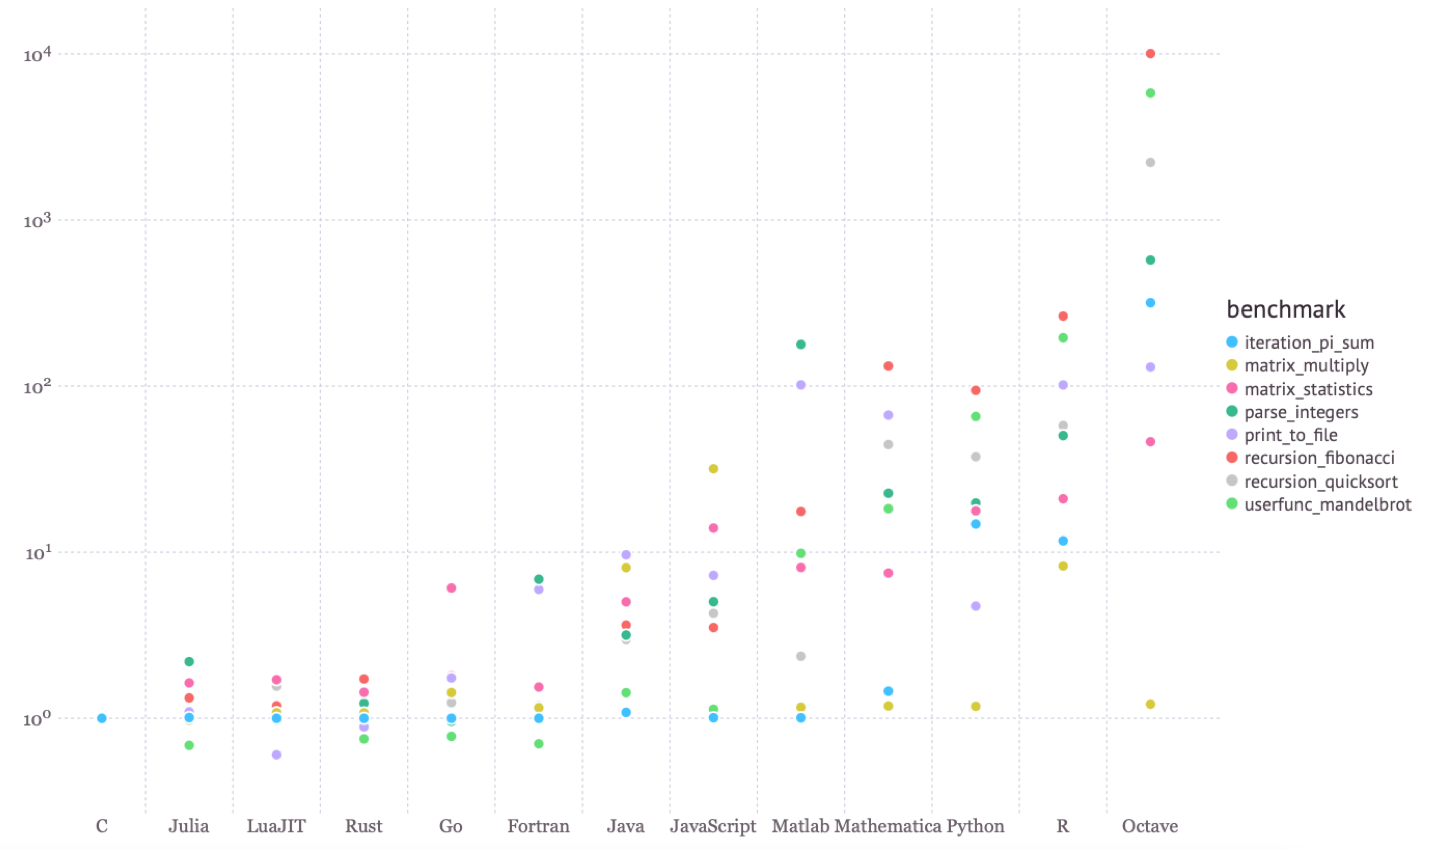
\includegraphics[width=0.8\textwidth]{figures/chapter-2/julia.png}
    \caption{Julia benchmarks from \href{https://julialang.org/benchmarks/}{Julia website}}
    \label{fig:julia}
\end{figure}






%%%%%%%%%%%%%%%%%%%%%%%%%%%%%%%%%%%%%%%%%%%%%%%%%%%
%                  2. Table
%%%%%%%%%%%%%%%%%%%%%%%%%%%%%%%%%%%%%%%%%%%%%%%%%%%
\section{Table}

Here are a table example.

\begin{table}[h]
    \centering
    \caption{Ambient noise package}
    \label{tab:noise-package}
    %\begin{tabular}{c|cccp{6em}p{3em}c}
    \begin{tabular}{m{2cm}<{\centering}m{2cm}<{\centering}m{2.5cm}<{\centering}m{2.5cm}<{\centering}m{1cm}<{\centering}}
        \toprule
        Package   & Language & Multiprocessing & Multithreading & GPU   \\

        \midrule
        SeisNoise.jl &  Julia & \checkmark  & \checkmark & \checkmark \\
        NoisePy & Python & \checkmark & & \checkmark \\
        Mirmex &  C++ & &  \checkmark & \checkmark \\
        CC-FJ  & Python with C++ & & \checkmark  & \\
        NoiseCorr & MATLAB & \checkmark & & \\
        \bottomrule
    \end{tabular}

\end{table}





%%%%%%%%%%%%%%%%%%%%%%%%%%%%%%%%%%%%%%%%%%%%%%%%%%%
%                  3. algorithm
%%%%%%%%%%%%%%%%%%%%%%%%%%%%%%%%%%%%%%%%%%%%%%%%%%%

\section{Algorithm}

Here are an algorithm example.

\begin{algorithm}[h]
    \SetAlgoLined
  
    Choose initial $m_0$,$S(m_0)$\;
    Compute $\pi_{post}(m|d_{obs})$\;
    \For{$k = 0,\dots,N-1$}{
        \eIf{$k<N_k$}{
            Define $S(m)=S_{time}(m)$\;
        }{
            \If{$k<N_k+M_{mag}$}{
                Estimate $M_0$ with formula XX\;
        }
        Define $S(m)=S_{time}(m)$\;
        }
        Draw sample $y$ with random walk with formula 17\;
        Compute $\pi_{post}(y|d_{obs})$\;
        Compute $\beta(m_k,m_{k+1}) = min \biggl\{ \frac{\pi_{post}(m_{k+1}|d_{obs})} {\pi_{post}(m_{k}|d_{obs})}, 1   \biggr\}$ \;
        Draw random number $u \sim u([0,1])$\;
        \eIf{$u<\beta(m_k,m_{k+1})$}{
            Accept: set $m_{k+1}=y$\;
        }{
            Reject: set $m_{k+1}=m_k$\;
        }
    }
    \caption{MCMTpy algorithm to sample proposal distribution $\pi_{post}(m|d_{obs})$}
    \label{algo:MCMTpy}
\end{algorithm}






%%%%%%%%%%%%%%%%%%%%%%%%%%%%%%%%%%%%%%%%%%%%%%%%%%%
%                  4. Code
%%%%%%%%%%%%%%%%%%%%%%%%%%%%%%%%%%%%%%%%%%%%%%%%%%%

\section{Code}


%%%% directly %%%%
% Insert Python code showing below.

% \begin{pythoncode}
% import numpy as np
% """
%     Annotation here.
% """
% # Annotation here.
% def main():
%     for i in range(0,10,1):
%         if i == 1:
%             print("Hello world")

% # Annotation here.
% if __name__ == "__main__":
%     main()
% \end{pythoncode}


%%%% from file %%%%
Insert Python code from files.





\clearpage % Conclusions




%%%%%%%%%%%%%%%%%%%%%%%%%%%%%%%%%%%%%%%%%%
% bib && appendices
%%%%%%%%%%%%%%%%%%%%%%%%%%%%%%%%%%%%%%%%%%
\backmatter
\appendix
\cleardoublepage
\addcontentsline{toc}{part}{Appendices}
\chapter{Appendix-1}

Here are the Appendix-1.

\bibliography{bib/pub}
\addcontentsline{toc}{part}{Bibliography}



\includepdf[pages={2}]{coverpage/TORRES_coverpage.pdf}
\end{document}
